%% aspas é assim ``bababba''
%% marcos 88970158

%\documentclass[draft]{ppgmus}
\documentclass{ppgmus}
\usepackage{textcomp}
\usepackage{kchicago}
\interfootnotelinepenalty=10000
\clubpenalty=10000
\widowpenalty=10000

\newcommand{\pd}{PD}
\newcommand{\objeto}[1]{[#1\texttildelow]}
%teste pra arrumar figs: http://www.tex.ac.uk/cgi-bin/texfaq2html?label=floats
\renewcommand{\topfraction}{.85}
\renewcommand{\bottomfraction}{.7}
\renewcommand{\textfraction}{.15}
\renewcommand{\floatpagefraction}{.66}
\renewcommand{\dbltopfraction}{.66}
\renewcommand{\dblfloatpagefraction}{.66}
\setcounter{topnumber}{9}
\setcounter{bottomnumber}{9}
\setcounter{totalnumber}{20}
\setcounter{dbltopnumber}{9}




%% newcommand e uma macro local

\autorbib{Figueiró, Cristiano Severo}
\titulo{SinCoPA- Sistema Interativo de Composição,Performance e Análise - Técnicas, Reflexões e Poéticas}
\autor{Cristiano Severo Figueiró}
\ano{2010}
\tipo{doutorado}
\area{Composição}
\lugar{Salvador}
\orientador{Prof. Dr. Pedro Ribeiro Kröger Jr.}
\mes{Maio}

%\cutter{S192}
%% Palavras-chave com termos da biblioteca nacional
%%\chavei{Composição (Música) --- Programas de computador}
%%\chaveii{Música --- Análise, apreciação}
%% Para funcionar em qualquer ppgmus.cls
%%\chaveiii{}
%%\chaveiv{}

%% Palavras-chave corretas
% \chavei{Composição musical}
% \chaveii{Contornos musicais}
% \chaveiii{Quinteto de sopros}
% \chaveiv{Computação musical}
%\cdu{78.02}
%\cdd{781.3}

%\dataDefesa{Salvador}
%\localDefesa{28 de novembro de 2008}

%\figuraTermo{termo-de-aprovacao}
%\escala{.2}

% \bancaiNome{Pedro Ribeiro Kröger Júnior}
% \bancaiTitulo{Doutor em Composição}
% \bancaiEstudo{Universidade Federal da Bahia (UFBA)}
% \bancaiAtuacao{Universidade Federal da Bahia}

% \bancaiiNome{Jamary Oliveira}
% \bancaiiTitulo{Doutor em Composição}
% \bancaiiEstudo{\textit{University of Texas at Austin}, EUA}
% \bancaiiAtuacao{Universidade Federal da Bahia}

% \bancaiiiNome{Liduino José Pitombeira de Oliveira}
% \bancaiiiTitulo{Doutor em Composição}
% \bancaiiiEstudo{\textit{Louisiana State University System}, EUA}
% \bancaiiiAtuacao{Universidade Federal da Paraíba}


%\titulofonte{Qualificativo}
\begin{document}
 


\capa
\begin{dadosTese}
Texto entregue como requisito parcial para Processo de Doutoramento.
\end{dadosTese}


\title{Tese}
\author{Cristiano Figueiró}



\tableofcontents

\newpage

% \begin{abstract}
%  
% A criação de música interativa é uma tarefa que envolve diversos 
% conhecimentos como técnicas de composição musical, síntese sonora,
% análise e processamento de sinal digital e design de interface.
% Nos últimos anos, diversos projetos vem sendo desenvolvidos e adotados
% pela comunidade de compositores interessados em compôr música baseada
% na interação homem-máquina. Notadamente a linguagem Pure data (Pd),
% vem sendo amplamente adotada pela flexibilidade de extensão de objetos 
% e capacidade de se integrar a outras linguagens e soluções existentes
% no campo da computação musical. Pd é uma linguagem gráfica...
% 
% Mesmo possibilitando diversas soluções ao compositor, o Pd exige
% o estudo formal de sua gramática tal qual qualquer linguagem de 
% programação. Muitas das soluções apresentadas pela comunidade
% são específicas e dificilmente adaptáveis a problemas gerais de 
% composição.
% 
% Nesta pesquisa investigamos o problema da criação de uma biblioteca
% de utilitários que realizem a interação entre os conhecimentos necessários
% para criação de música interativa. A criação dessa biblioteca permite
% soluções híbridas interligando diversas outras bibliotecas gerais e
% específicas desenvolvidas pela comunidade. O uso da biblioteca
% propicia ao compositor uma rápida prototipagem em música interativa e 
% integração com outros fluxos de trabalho, ao mesmo tempo em que permite
% um estudo mais aprofundado da linguagem e customização da própria biblioteca
% apresentada aqui.
% 
% 
% 
% \end{abstract} 

\chapter{Introdução}
\label{sec:intro}


Essa pesquisa apresenta a busca por um modelo de composição e
performance de música interativa – evento sonoro gerado a partir da
performance de um músico sobre uma base de programas, materiais
estocados e análise das informações da performance em tempo-real. O
modelo é materializado na forma de um sistema computacional que seja
capaz de extrair informações diversas sobre a performance e
categorizar aspectos da performance musical e interagir com essa performance.


O sistema é construído com a linguagem \textit{Pure Data} (\pd). O Pd é uma linguagem gráfica orientada ao objeto que surgiu
como linguagem voltada para a criação de música eletrônica e nos últimos anos foi-se desenvolvendo inúmeras
bibliotecas de objetos especializados em modelos matemáticos, modelamentos de interface gráfica, diversas 
implementações
em processamento e análise em tempo-real de sinal de áudio, vídeo, rede e hardware. 
A análise dos dados da performance musical é construída usando objetos ``nativos`` e ``externals`` 
discussão que será
aprofundada no capítulo da metodologia. 
Todas as partes do sistema são construídas em Pd, no formato de objetos
modulares. Os objetos criados tem a função de agregar diversos outros objetos e organizar o fluxo de dados
de análise e performance num contexto que possibilite o re-uso em diferentes projetos e contextos de 
criação de música e arte interativa.Também são apresentados três protótipos de uso do sistema. A visão geral do
SInCoPA é a de uma biblioteca de objetos de Pd e sua documentação de uso, e um catálogo de protótipos e projetos
utilizando essa biblioteca que servem como campo de avaliação de possibilidades e experimentação sonora.


Foram usadas diversas bibliotecas externas ao Pd, algumas que são encontradas na distribuição pd-extended
\footnote{pd-extended é uma distribuição do Pd com várias bibliotecas externas já compiladas na maioria dos
sistemas operacionais existentes. É o principal ''fork`` do Pd, e possui versão estável e versão de desenvolvimento.
A história de desenvolvimento do Pd pode ser entendida como uma sequência de Forks levando a diferentes versões 
e estágios de desenvolvimento locais, como JMax, Max-Ircam, DesireData, etc...Essa pesquisa assume como padrão
a versão atual do pd-extended com algumas adições de bibliotecas de objetos feitos em Pd e alguns objetos codados
em C e compilados como objetos de Pd.}, 
e outras contribuições da comunidade de desenvolvedores.

\section{Problemas}

%% aqui mudar de "problemas" para "elementos" ou.. em:
%% 1) sons acústicos e eletrônicos
%% 2) notação de música interativa
%% 3) composição algorítmica
%% 4) poética da interação - referencias do flo menezes
%% 5) desenho de interface músico-instrumento-computador
%% 6) interação, simulação, acompanhamento, complemento,
%% 7) IA, interação para além do controle




A criação de música interativa é uma tarefa que envolve diversos 
conhecimentos como técnicas de composição musical, síntese sonora,
análise e processamento de sinal digital e design de interface.

Nesta pesquisa investigamos o problema da criação de uma biblioteca
de utilitários que realizem a interação entre os conhecimentos necessários
para criação de música interativa.


Diversos problemas derivam da intersecção entre descrições simbólicas
de composição e estruturação musical como nota, acorde, motivo e 
especificações de síntese sonora como modulação, envelope e formas de onda.
Alguns problemas são conceituais e demandam um universo próprio de 
pesquisa como por exemplo a detecção automática de começo e fim de
frases melódicas. Outros problemas são técnicos e prevêem uma depuração
na programação como por exemplo a sincronia entre as mensagens de controle de parâmetros
e o processamento de blocos de áudio. 



\subsection{Composição e Programação}
  

% Se estabeleceu que o objetivo é encontrar
% uma intersecção entre os procedimentos de pesquisa em computação musical e 
% a poética composicional.


O paradigma composicional no Csound\footnote{Csound é um ambiente de programação
sonora open-source e baseado na linguagem C - www.csounds.com} pode ser visto como semelhante ao
trabalho tradicional do compositor que descreve eventos através de
dois arquivos: uma orchestra e um score, onde no primeiro são
descritas as qualidades fixas do timbre e no segundo os eventos e os
parâmetros dinâmicos do timbre. A arquitetura de programas como Max e
Pd, a primeira vista pode ser vista como simples e convidativa pelo
fato de possibilitar uma programação intuitiva e parecer com um
fluxograma. Mas logo se dão as primeiras dificuldades pelo fato de o
paradigma da linguagem ser muito calcado na performance em tempo-real
causando a dificuldade de organização dos dados composicionais, como
notas, acordes, eventos e mudanças de parâmetros de síntese.

Os músicos tem sua formação baseada na notação musical tradicional que
estabelece uma cadeia de binômios de parâmetros de estruturação sonora
\cite{zampronha00:notacao} como altura versus ataque, duração versus
articulação ou métrica versus expressão. O sistema da notação
tradicional tem uma estrutura que possui uma sequencialidade temporal
dos eventos implícita. A migração dos músicos para ambientes de
composição e design sonoro como Csound \cite{boulanger00:csound} tende
a ser mais natural pela adaptação de um tipo de estrutura temporal
(partitura) para outro (Score), e também pela oposição binária entre
``orchestra'' e ``score''. No Csound, a base de dados é chamada
``Score''. Scores em Csound consistem na maioria das vezes em
``notas'', que são comandos para um sintetizador (orchestra). O score
é essencialmente uma sequência temporal. Uma possível sequência
temporal em Csound pode ser vista:

\begin{verbatim}
;orchestra
instr 1
  k1  linen 10000, .2, p3, .5
  a1  oscil k1, p4, 1
      out a1
endin

;score
f1 0 2096 10 1 .2 .3
i1 0 1 440
i1 1 1 660


\end{verbatim}

Programadores também são acostumados com linguagens de programação que
tem sua gramática baseada na sequencialidade das ações. A vantagem de
usar uma ferramenta de síntese embutida em uma linguagem de
programação é que se pode ter uma flexibilidade muito maior na criação
relações entre os elementos devido a possiblidade de criar novas
abstrações. Abaixo temos um exemplo de código em Comonn lisp music.

\begin{verbatim}
(definstrument simp (start dur frequency amp \&optional
                    (amp-env '(0 0 .5 1.0 1.0 0)))
  (multiple-value-bind (beg end) (times->samples start dur)
    (let ((osc (make-oscil :frequency frequency))
          (amp-env (make-env :envelope amp-env :scaler amp
                             :dur dur)))
      (run 
       (loop for i from beg below end do
            (outa i (* (env amp-env) (oscil osc))))))))
\end{verbatim}

\begin{verbatim}
(with-sound ()
  (simp 0 1 440 1)
  (simp 1 1 660 1))
\end{verbatim}

\begin{verbatim}
(with-sound ()
  (loop for freq from 100 to 1000 by 100
     for dur from 0 to 10 do
       (simp dur 1 freq 1))
\end{verbatim}

Se formos tentar implementar esse código em Pd. Podemos encontrar algo assim: 

\begin{figure}
  \centering
  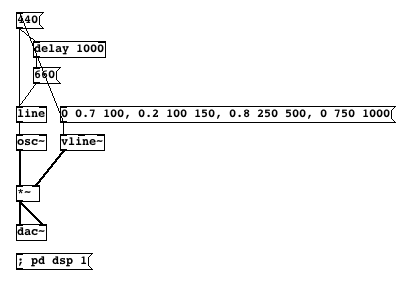
\includegraphics[scale=.5]{exemplopd1}
  \caption{2 notas num oscilador simples}
  \label{fig:exemplopd1}
\end{figure}

O fato do Pd ser uma linguagem gráfica possibilita uma facilidade de
descrição do processo de síntese sonora pelo fato de que o próprio
código é semelhante ao fluxograma tradicional de representação da
síntese.
% (inserir figura de fluxograma)

 A estrutura de um fluxograma
possui uma sequencialidade implícita (da saída final até os parâmetros
de cada gerador), mas não explicita como vão ser manipulados os
parâmetros nem qual será a duração da música.

Os ambientes Max/Msp e Pd são construídos sob o paradigma do ``envio
da mensagem'' que não necessariamente possibilita que a linguagem seja
adequada para o estoque e a recuperação de dados. O usuário é
praticamente forçado a colocar os dados dentro de conteiners - bases
de dados, essencialmente - e a usar um leque de objetos como
acessórios para estocar e recuperar dados dentro do controle de
passagem de mensagens em tempo-real.

A abordagem do Max/ Msp quanto aos dados é ao mesmo tempo simples e
evasiva: objetos especiais de armazenagem de dados como
\textit{table}, \textit{qlist}, dentre outros são disponibilizados. Os
dados são essencialmente colocados dentro de objetos conteiners, e
para cada tipo de objeto-conteiner uma abordagem particular é colocada
para sua estocagem, edição, interface e comunicação com o resto do
patch.

A recuperação de dados (a grande maioria das transações de bases de
dados) é a pior qualidade do Max porque mensagens não tem valores de
retorno. Por exemplo, uma caixa de número manipulada com o mouse não
retorna os dados da manipulação, que devem ser recuperados com outros
objetos). Os dados recuperados devem ser mandados como uma mensagem
separada de retorno. Isso leva muitos programadores de Max a achar
soluções diferentes que facilite a interação do patch com o nível
composicional.

A idéia original por trás da criação do Pd foi remover a barreira
entre a computação dirigida por eventos em tempo-real (como no estilo
do Max de passagem de mensagens) e dos dados (como em pontos num
gráfico ou notas numa partitura). Em Pd os dois (caixas de objetos e
estruturas de dados) podem facilmente coexistir em uma mesma janela.
Essa ``promiscuidade'', no entanto, não acaba deixando os objetos
funcionais e os dados intimamente conectados. De fato, no design
presente, o acesso aos dados tem que ser feito através de uma
sequência de objetos como acessórios .

Em relação a essa divisão do aspecto ``performático'' e
``composicional'' do Pd, Miller Puckette explica que

\begin{quote}
  in its most succinct form, the problem is that, while we have good
  paradigms for describing processes (such as in the Max or Pd
  programs as they stand today), and while much work has been done on
  representations of musical data (ranging from searchable databases
  of sound to Patchwork and OpenMusic, and including Pd's unfinished
  data editor), we lack a fluid mechanism for the two worlds to
  interoperate. \cite{puckette04:divide}
\end{quote}

Dentro de uma proposta de trabalho de composição de música interativa,
o objetivo musical deve ser o mais claro possível de maneira que o
código emerja naturalmente dos problemas musicais ao invés de
atrapalhar mais ainda os problemas composicionais. Abordando o assunto
a partir de uma visão didático-metodológica um primeiro projeto
composicional em Pd, deve compreender a clara distinção entre os
aspectos performáticos e composicionais do ambiente. Um primeiro
projeto composicional deve dar conta de fornecer elementos para o
estabelecimento de uma metodologia apropriada de controle dos eventos
temporais. A proposta aqui é a de abordar o uso prático e algumas
possíveis implementações em Pd que apontem para a criação de
composições interativas mistas de maior porte. O objetivo é dispôr de
elementos que possam apontar para uma possível poética composicional.


\subsection{Análise de áudio}


- MIDI como padrão

- problema do violão e guitarra - citar o miller no patch for guitar


\subsection{Segmentação e Classificação}

segmentação automática estática ou dinâmica

segmentação e classificação automática - redes neurais ou outro algoritmo

segmentação com controle do músico - teclado hackeado ou
algum botão com arduino criando um hyper-instrumento


\subsection{Interação e Automação}


\subsection{Poética da interação}


Rodolfo Caesar:

\begin{quotation}
 Nos loops de áudio quanto mais semelhança entre as partes final e inicial, mais mascarada fica a
emenda. Quanto mais disfarçada a parte da ‘cola’, mais garantido o efeito de um ‘sem fim’. A finalidade
desta emenda bem-feita manifesta premonitoriamente (no século XIX), o desejo de ‘imersão’ de algumas
artes ‘digitais’, ‘multimídias’ ou ‘tecnológicas’, projeto típico de décadas finais do século XX e início do
XXI. O sonho da ‘obra de imersão total’ – que portanto depende de um confinamento e um mascaramento -
é criteriosamente representado no filme ‘Brainstorm’ (1983), de Douglas Trumbull, no qual um grupo de
cientistas inventa um gravador que registra integralmente as emoções humanas. O grau máximo e total de
satisfação onanista é perseguido por um dos cientistas - personagem representando o mau uso da ciência -
que finalmente realiza seu super-loop:
Clip: trecho de ‘Brainstorm’, em que se vê o ‘mau’ cientista aprisionado ao loop de seu orgasmo, gravado na
companhia de uma prostituta, que não receberá royalties pelo uso de sua imagem.
\end{quotation} 

Flo Menezes:

\begin{quotation}

A essência da fusão e do contraste

Para haver fusão entre as escrituras instrumental e eletroacústicas,
será necessário que haja \textit{transferências localizadas} de 
características espectrais de uma esfera de atuação à outra.
Aquilo que se funde com outra coisa, assim o faz pela \textit{similaridade
absoluta}, com esta outra coisa, de ao menos um aspecto de sua 
constituição. Nesse sentido, tratando-se de sons eletroacústicos 
pré-elaborados em estúdio, a eleição do material constitutivo de partida
adquire grande relevância: será mais plausível trabalhar, sobre suporte,
com sons oriundos dos próprios instrumentos do que com proveniências
díspares, sem qualquer relação de origem com a materialidade corpórea
dos instrumentos utilizados. Ainda que as transformações em curso possam ser
bem drásticas, o uso de material constitutivo similar faz com que
haja preponderância em conservar algum aspecto energético que confira
identidade às texturas sonoras resultantes.
....
Como quer que seja, na fusão instaura-se uma condição de \textit{dúvida}.
Em certa medida, fusão implica propositadamente, da parte do compositor,
\textit{confusão} para o ouvinte....o ouvinte recai em constantes dúvidas
acerca da natureza daquilo que se ouve: se advém do instrumento ou da 
emissão eletroacústica, se se opera ao vivo uma dinamização espacial, harmônica
, tímbrica e temporal da escritura instrumental ou se será defronte de
estruturas pré-elaboradas em estúdio, constituidas a partir dos próprios
instrumentos ou a estes timbricamente correlatas. Em relação a proveniência
sonora, quanto mais ``confuso'' estiver o ouvinte em face daquilo que
o ouve, tanto mais ele sentirá como efetivamente integradas as partes
constitutivas da obra mista; os "dois planos" pressupostamente independentes
e unidos apenas por contingência, aos quais os críticos da música mista
faziam referência, passam a ser percebidos como um \textit{único plano},
essencialmente \textit{diagonal} às linhas estanques da emissão instrumental
ou da difusão puramente eletroacústica; a emissão instrumental passa,
então, a ser efetivamente potencializada no espaço acústico pelos recursos 
eletrônicos. Ainda que de forma alguma hegemônico, o \textit{estado de
dúvida} traduz-se como momento supremo da interação.

O contraste, por sua vez, ancora-se sobretudo na diferença e na 
\textit{distinção absoluta}. Em seus momentos mais acentuados, faz com
que a emissão instrumental ou a eletroacústica assumam o papel estrutural
do silêncio ou, ao contrário, adquiram autonomia temporal e até mesmo
excludente com relação à outra esfera sonora.


copiar mais a página 388 (10.png)

- > usar essa página como exemplo do uso da análise como motor 
composicional

\end{quotation}









\section{Referências}

Alguns projetos relacionados podem servir como fonte de inspiração pra
a presente pesquisa como o Cypher \cite{rowe93:interactive}   de Rowe que usa a metáfora da
sociedade da mente de Minsky na forma de músicos artificiais dentro de
um sistema multi-agente - o Meta-Cypher inclui múltiplos ouvintes e
performers além de um meta-ouvinte.  O Drum Circle \cite{eigenfeld07:drum} é um sistema escrito em Max/MSP e explora o uso de
multi-agentes sobre uma rede local onde cada agente emula um
percussionista improvisando em um grupo de tambores, tendo como
resultante um ritmo evolutivo.

Um dos projetos mais amplos nessa área é o projeto Omax Brothers \cite{assayag06:omax}
desenvolvido no Ircam. Um sistema multi-agente criado para
improvisação musical entre homem-máquina que aprende em tempo-real com
o performer humano. O núcleo da improvisação é baseado em modelamento
de sequência e aprendizado estatístico. O sistema envolve uma
arquitetura híbrida usando dois ambientes populares para composição e
performance, OpenMusic (baseado em Lisp) para modelamento e
programação de alto nível e Max/MSP para a performance do sistema e
processamento de áudio em tempo-real.

Da parte musical diversas peças motivaram o desenvolvimento desse trabalho como as peças
''Jupiter'' e ''En Echo'' de Philippe Manoury para flauta e computador e soprano e computador respectivamente.
Essas músicas foram desenvolvidas em colaboração com Miller Puckette o criador do Max e do Pd. As duas 
peças empregam o uso da técnica de ''Score-follower``, uma técnica que também foi explorada por mim em
meu trabalho de mestrado, na peça ''Enquanto eles riem``(2005) para Clarinete e computador com Max/MSP.

\section{Processo}

O desenvolvimento cronológico dessa pesquisa levou a um primeiro momento de intenso aprendizado
dos detalhes e técnicas de programação com Pd, desenvolvendo materiais didáticos, traduções, e uma
sequência de estudos interativos usados em peças musicais e performances sonoras. Um exemplo pode ser visto
na figura \ref{flauta2007}, onde um Score-follower controla os parâmetros de 
processamento do som da flauta e harmoniza certos trechos da peça de acordo com as notas da flauta.

\begin{figure}
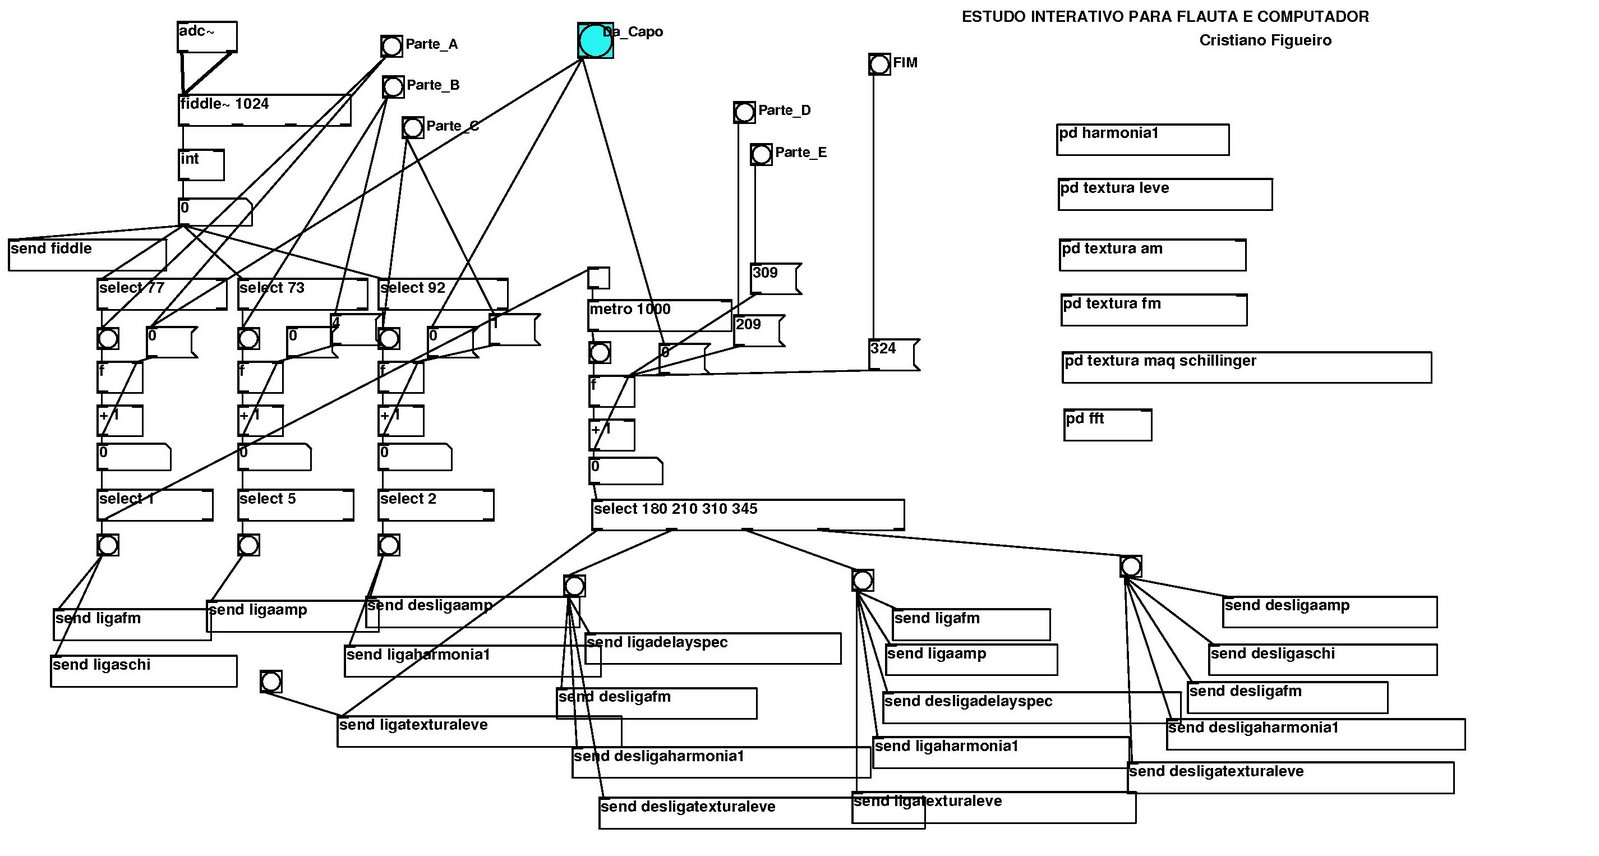
\includegraphics[scale=.3]{flauta2007}
\caption{estudo interativo pra flauta e computador (2007)}
\label{flauta2007}
\end{figure} 

A comunidade de desenvolvimento do Pd é muito ativa, e explicitamente projetos open-source
se esforçam para mudar a condição do interessado no software de usuário passivo a participante ativo do desenvolvimento
e das decisões coletivas sobre os caminhos que a linguagem deve tomar. Esse  fator acarretou na
organização de 2 eventos com desenvolvedores e forte interação com a comunidade\footnote{III International
Convention of Puredata (PdCon) em São Paulo e o I Simpósio Internacional de Interatividade nos Sistemas
Computacionais Livres (wwww.iscl2009.wordpress.com) em Salvador em 2009.}, desenvolvimento de peças interativas para instrumentos
tradicionais e computador, oficinas de extensão, participação em desenvolvimento de projetos coletivos
usando pure data, como navalha e mimosalib usada nos protótipos.


\subsection{Redes Neurais artificiais}

% Na prática o sistema funcionará em duas instâncias: num primeiro momento
% as redes precisam ser treinadas. Nessa fase o músico executa uma performance, esse
% áudio é captado, analisado e colocado numa base de dados que vai servir como
% arquivos de treinamento das redes. O segundo momento será o momento da performance interativa,
% onde o sistema vai responder ao estímulo do músico comparando a análise de sua performance em tempo-real
% com esse banco de dados previamente estocado.
% Uma visão geral do sistema pode ser vista na figura \ref{geral} onde 
% podemos ver o fluxo geral dos dados ao longo das partes do sistema. Podemos ver
% que a resposta do sistema ao estímulo do músico depende da resposta das redes que 
% procuram por padrões. O resultado das redes distribui pesos no mecanismo de decisões que por sua vez aplicam processos de transformações no material exposto pelo músico e armazenado no banco de dados.




\begin{figure}
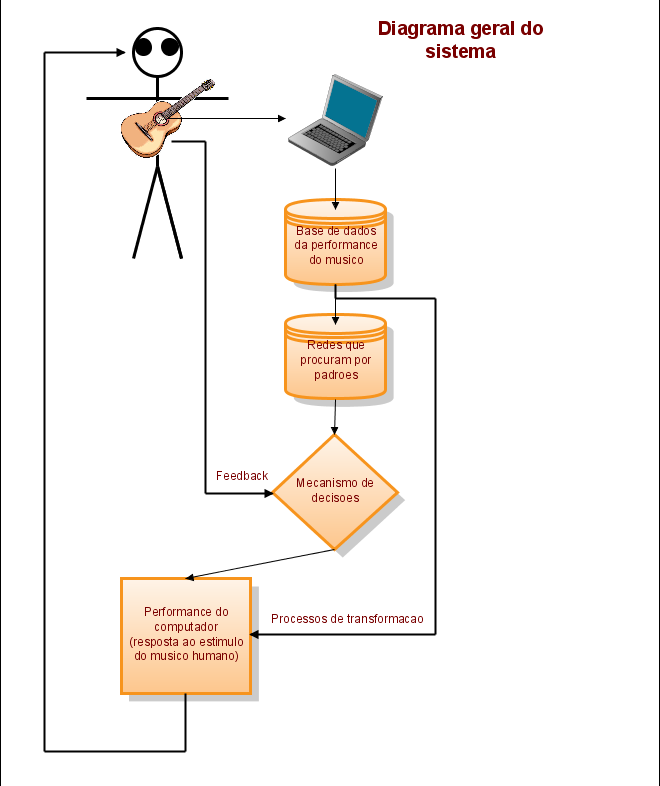
\includegraphics[scale=.7]{geral}
\caption{Diagrama geral do sistema}
\label{geral}
\end{figure}



%colocar parágrafo de como que está agora

%Na figura\ref{mecanismo}

\begin{figure}
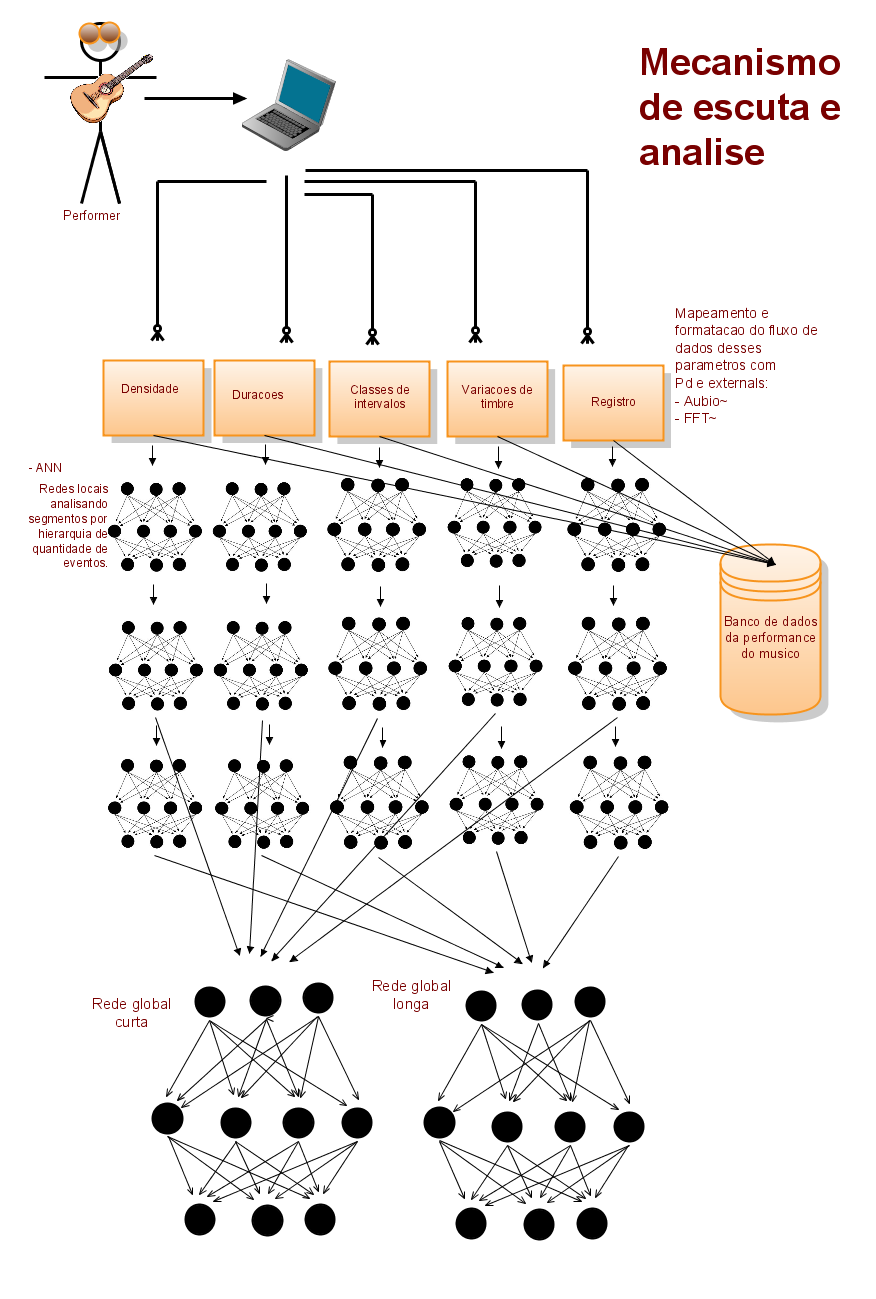
\includegraphics[scale=.7]{escuta}
\caption{Mecanismo de escuta e análise}
\label{escuta}
\end{figure}

%%%%%% artigo pdcon09

INTRODUÇÃO
A pesquisa em computação musical tradicionalmente se utiliza de desenvolvimentos em redes neurais artificiais 
(ann – artificial neural networks), agentes inteligentes artificiais e outros ramos da pesquisa em inteligência 
artificial (IA); a produção musical oferece ótimos casos - teste para a pesquisa em IA. 
Em determinado momento, a pesquisa convergiu para o desenvolvimento de um sistema baseado em redes neurais.
Essa seção expõe esse momento da pesquisa, descrevendo como se pode trabalhar com redes neurais artificiais com Pd.

A figura \ref{escuta} representou o planejamento inicial do projeto onde podemos observar como a 
análise do áudio foi separada nos parâmetros de
densidade, durações, classes de intervalos, variações de timbre e registro. Cada parâmetro passaria
 por uma cadeia de redes locais de tamanhos diferentes que seriam agrupadas em duas 
redes globais também de tamanhos diferentes.

\begin{figure}
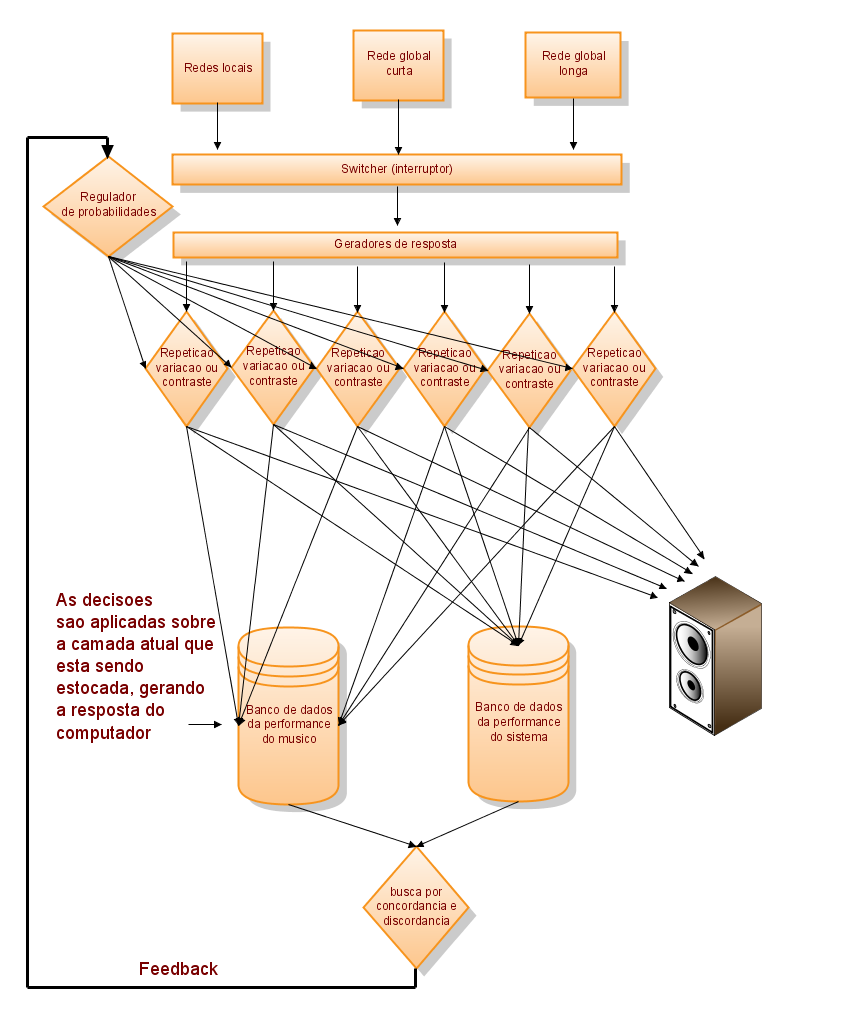
\includegraphics[scale=.7]{mecanismo}
\caption{Mecanismo de funcionamento de um sistema interativo baseado em redes neurais}
\label{mecanismo}
\end{figure}




A idéia era se aproximar de modelos cognitivos, tentando simular situações de aprendizado musical.
As habilidades de músicos humanos em fluidez de ação, capacidade de 
resposta a situações novas e referências culturais, transformam a capacidade de interação dos sistemas computacionais 
numa árdua tarefa. Na prática o sistema funcionaria em duas instâncias: num primeiro momento as redes precisam ser 
treinadas. Nessa fase o músico executa uma performance, esse áudio é captado, analisado e colocado numa base de dados 
que vai servir como arquivos de treinamento das redes. O segundo momento será o momento da performance interativa, 
onde o sistema vai responder ao estímulo do músico comparando a análise de sua performance em tempo-real com esse 
banco de dados previamente estocado. Uma visão geral do sistema pode ser vista na figura \ref{mecanismo} onde podemos ver o fluxo 
geral dos dados ao longo das partes do sistema. Podemos ver que a resposta do sistema ao estímulo do músico depende 
da resposta das redes que procuram por padrões. O resultado das redes distribui pesos no mecanismo de decisões que por 
sua vez aplicam processos de transformações no material exposto pelo músico e armazenado no banco de dados.
   O fato do sistema ter como paradigma a criação de música em tempo-real ainda requere uma grande dimensionalidade de 
descrições, rápido aprendizado, respostas e efetiva capacidade de antecipação. 


CARACTERÍSTICAS DO SISTEMA
O sistema vai ser construído utilizando-se a linguagem Pure Data (Pd). O Pd é uma linguagem gráfica orientada ao objeto. 
A análise do áudio de entrada vai ser feita pelos objetos [fiddle\texttildelow] , [sigmund\texttildelow], [fft\texttildelow]
 e também pela biblioteca Aubio[8] que 
é uma biblioteca de funções de análise de áudio escrita em C e transcrita para funcionar como uma biblioteca extra (
external) do Pd. Os resultados das análises de áudio será passado por um sistema de redes neurais artificiais, 
construídos com a biblioteca FANN [1] portada para ser usada como uma external de Pd. As redes neurais serão organizadas 
por ordem de tamanho de segmentos temporais. Por exemplo, a primeira rede vai procurar por padrões a cada 20 segundos e 
mandar os resultados para a segunda rede que vai avaliar a presença de padrões a cada 60 segundos e assim por diante. 
Esse processo será feito em todos parâmetros descritos. Os resultados desssas redes serão enviados para um banco de dados
 que vai ser comparado com o banco de dados usado no treinamento das redes. A comparação entre os bancos de dados do 
treinamento e da performance em tempo-real vai regular as decisões de resposta do sistema. Um diagrama geral do 
funcionamento do sistema pode ser visto na figura 1.
  Pode-se, portanto, definir que uma boa abordagem de pesquisa em sistemas musicais interativos engloba um vasto 
campo multidisciplinar realizando uma fusão de pesos iguais entre as áeas de psicologia cognitiva, computação e teoria 
da composição musical. Essa fusão se dá de maneira pragmática, materializada num sistema de software e hardware, 
capaz de responder musicalmente a estímulos musicais e também capaz de aprender e analisar comportamentos musicais 
do músico tendo conhecimento de seu passado, presente e assim podendo projetar o futuro.
 ATUAL ESTÁGIO DA PESQUISA

 Fann 

No primeiro experimento da pesquisa  foi usado o external ann-mlp com o objetivo de detectar  em tempo-real padrões 
rítmicos pré-estabelecidos na fase de treinamento da rede.
   Redes neurais e outras técnicas de inteligência artificial são ideais para experimentos com detecção de padrões em 
tempo real  pelo fato de retornarem percentuais de semelhança com dados pré-analisados e estocados numa base de dados, 
ao invés de respostas objetivas como resultado.

Figura 1. Diagrama geral do sistema
 O principal elemento explorado  nesse primeiro experimento foi a variação de andamento. Uma das principais 
características de um diálogo musical é o fato dos músicos reconhecerem facilmente padrões rítmicos independente do 
andamento em que são apresentados.. Para isso é necessário que seja levado em consideração a distância temporal entre 
ataques de eventos sonoros ao invés da duração desses eventos ou do posicionamento temporal dentro da duração total da 
performance.

Figura 2 . patch central
 Segmentação rítmica
Para o trabalho de segmentação rítmica foi usada a biblioteca Aubio para identificar os ataques (onsets) de eventos 
sonoros. No patch principal podemos ver a maneira como se dá a detecção de ataques com o objeto [aubioonset\texttildelow] que retorna 
um bang para cada ataque de evento. Na figura 2 vemos o patch central com o objeto  [aubioonset\texttildelow] recebendo um fluxo de 
dados de áudio e respondendo com bang em tempo-real para cada ataque reconhecido.
   Para o primeiro experimento dessa pesquisa foi escolhido uma
metodologia de segmentação agrupando conjuntos de quatro ataques. Na figura 3 podemos ver no patch como foi implementado 
o agrupamento de cada quatro  ataques dentro do sub-patch pd contador de ritmos e estocando beta.
Figura 3. pd contador de ritmos e estocando beta
No âmbito geral do sistema essa estrutura vai ser a base da segmentação dos parâmetros do áudio de entrada. Esse método 
servirá tanto para  a criação dos arquivos de treinamento das redes quanto para a segmentação em tempo-real.

 Treinamento e performance das redes
As redes neurais artificiais funcionam em dois tempos, o treinamento e a performance. No treinamento as redes os pesos e 
dos padrões de maneira a criar um arquivo de treinamento que funciona como um banco de dados . No arquivo de treinamento 
podemos editar manualmente e identificar e rotular os padrões de maneira a refinar a base de dados. Nesse experimento foi 
desenvolvido um subpatch que cria automaticamente o arquivo de treinamento, que determina a quantidade de neurônios da 
rede, número de padrões a serem estocados e a quantidade de elementos de cada padrão.
   No experimento em questão foi usado um arquivo de áudio com um timbre percussivo e ataques bem claros. Esse arquivo 
contém 3 padrões rítmicos apresentados 3 vezes com  andamento diferentes. No resultado observamos que mesmo quando se 
altera o andamento, as redes continuam a detectar os padrões, porque durante a fase de treinamento os padrões foram 
apresentados diversas vezes em andamentos diferentes.

Nessa fase inicial, a implementação do reconhecimento de padrões tem gerado uma série de 
questões como: Qual o tamanho e quantas melodias/motivos quero que o programa reconheça? O programa 
deve fazer um reconhecimento estrito ou pode realizar uma classificação de aproximação ou 
similaridades? As melodias/motivos terão um tamanho fixo de notas ou tempo, ou serão variáveis? 
O que acontece se um motivo curto é um sub-conjunto de um motivo maior?




\subsection{Composição algorítmica e interação}



Aqui falar do RTC + MEPSOM

Falar das razões da pesquisa de termos dado um passo atrás, desistido
das redes neurais e focado num sistema estável bem documentado sobre todos
os componentes de um sistema interativo
 

% Pode-se, portanto, definir que uma boa abordagem de pesquisa em sistemas musicais interativos engloba um vasto campo 
% multidisciplinar realizando uma fusão de pesos iguais entre as áeas de psicologia cognitiva, computação e teoria da 
% composição musical.


\subsection{Papel do músico na interação homem-máquina}

* meu background como instrumentista e depois compositor

* instrumentista: o instrumento como "cola" sonora - gesto da gestalt ( "boa continuidade") de querer
completar os espaços em branco...ou dar significado para os espaços em branco

* compositor: a perda do "controle" composicional...a autoria já não é mais minha...
é minha e do computador...




O desenvolvimento de um sistema dessa natureza envolve um tipo de conhecimento que envolve técnica de
 composição, análise, performance e computação.
 Essa fusão se dá de maneira pragmática, materializada num sistema de software e hardware, capaz de 
responder musicalmente a estímulos musicais e também capaz de aprender e analisar comportamentos musicais do músico tendo 
conhecimento de seu
passado, presente e assim podendo projetar o futuro. A performance desse tipo de situação musical também leva a um  de questões
de como o sistema se comporta em diversas situações de hardware diferentes e qual 
o nível de estabilidade dos aplicativos na prática.



%% ligar esse último parágrafo com o tema dessa introdução

%% parágrafo de conclusão

\chapter{Revisão Bibliográfica}
\label{sec:rev}

O conceito de interação entre uma performance musical e computador vem
sendo definido nas últimas 3 décadas, e possui diferentes nuances de definição
a depender do contexto de idioma e prática musical a que se refere e a tecnologia
em que é implementada. A descrição ''sistemas musicais interativos``, é um
termo introduzido no livro \textit{Interactive Music Systems} 
\cite{rowe93:interactive} e definido como ''sistemas de música 
computacional em que as mudanças de comportamento são responsivas a um
estímulo musical``. Interação em um sentido mais global pode ser definida: 
  ''Interação tem dois aspectos:
tanto as ações do performer afetam a saída do computador, ou as ações do computador
afetam os resultados do performer`` \cite{garnett:2001}.

Isso pode ser comparado a comunicação entre músicos no modelo de  música de 
câmara tradicional onde dois ou mais músicos realizam música escrita, improvisada 
ou mista \cite{winkler93:interactive}.

Em relações interativas mais complexas, ``um compositor pode
delegar vários papéis a um computador num ambiente de música interativa. Ao
computador pode se dar o papel de instrumento, performer, regente, e/ou compositor.
Esses papéis podem existir  simultaneamente e/ou mudar continuamente''\cite{lippe:2002}.



A pesquisa em sistemas musicais interativos vem nos últimos anos
deixando de ser uma abstração teórica e se transformando em realidade
concreta. O corpo de áreas de pesquisa compreende temas como cognição
musical, computação e teoria e análise musical.


Podemos apontar a multi-disciplinaridade dessa pesquisa como pertencente 
ao escopo de uma disciplina genérica emergente denominada Design de Interação(ID).
%%o que é ID
A maioria dos tratados e especificações da ID se referem a interação para a web
e interação homem-máquina focada em paradigmas comerciais. Ainda que essa pesquisa busque
uma maior interação homem-máquina num nível de funcionalidade auxiliar a poética musical, algumas idéias e 
pensamentos da ID podem ser úteis na organização do desenvolvimento do SInCoPA. 
Como por exemplo os sete estágios da ação \cite{norman06:design} onde descreve que para 
descobrir o que torna a
execução de uma tarefa difícil é necessário examinar a
estrutura de uma ação. Ele propõe sete estágios: um para
meta, três para execução e três para avaliação. A seguir cada
estágio será detalhado.
Formalizar a meta – o primeiro estágio refere-se a decisão de
realizar alguma coisa, ou seja, estabelecer a meta a ser
alcançada. A meta é algo a ser atingido, e nem sempre é bem
definida.
Formalizar a intenção – de acordo com Norman as
metas não definem precisamente o que deve ser feito. Para
se transformar em ações as metas precisam ser traduzidas
em definições específicas do que deve ser executado, o autor
denomina essas definições de intenções. As intenções são
ações específicas que foram realizadas para atingir as metas.
Portanto, após determinar a meta a ser alcançada deve-se
determinar quais serão as ações a serem executadas para
atingir a meta estabelecida.
Especificar a ação – após definir as intenções, essas devem
ser traduzidas por um grupo de comandos internos, ou seja,
uma sequência de ações que possam ser desempenhadas de
modo a satisfazer a intenção. Ressalta-se que até esta etapa
tudo ocorre mentalmente.
Executar a ação – com a sequência de ações definidas,
deve-se colocar em prática o que foi estabelecido.
Ter a percepção do estado do mundo – esta fase esta
intimamente relacionada com a posterior (interpretar o estado
do mundo). Neste momento, deve-se perceber as alterações
ocorridas no ambiente que ocorre a ação.
Interpretar o estado do mundo – após a percepção deve-se
analisar e compreender o que ocorreu no ambiente em
questão.

Avaliar o resultado – por fim, deve-se comparar o resultado
obtido com a meta estabelecida para concluir se o que foi
planejado foi de fato alcançado.
Norman deixa claro que estes estágios não são regras,
são apenas um modelo aproximado para compreender como
os indivíduos fazem as coisas. Esses estágios podem facilmente
ser pensados como um método para um design do desenvolvimento 
de um projeto interativo. Apesar da presente pesquisa não usar de 
maneira sistemática esse método, esses estágios pode servir como
método de avaliação ao final do desenvolvimento.

Outra área emergente que possui muitas características em comum com essa
pesquisa é a disciplina que se chama ''Realidade Aumentada`` (RA), que é uma linha de pesquisa dentro da ciência da computação que lida com 
integração do mundo real e elementos virtuais ou dados criados pelo computador. Atualmente, a 
maior parte das pesquisas em RA está ligada ao uso de vídeos transmitidos ao vivo, que são 
digitalmente processados e “ampliados” pela adição de gráficos criados pelo computador.

A definição de Ronald Azuma 
sobre a Realidade Aumentada \cite{azuma97:ar} é uma descrição genérica que pode nos auxiliar na delimitação teórica. 
Ela ignora um subconjunto do objetivo inicial da RA, porém é entendida como uma representação 
de todo o domínio da RA: Realidade Aumentada é um ambiente que envolve tanto realidade virtual 
como elementos do mundo real, criando um ambiente misto em tempo real.
Azuma define a Realidade Aumentada como um sistema que:
\begin{itemize}
 \item combina elementos virtuais com o ambiente real; 
  \item é interativa e tem processamento em tempo real; 
  \item  é concebida em três dimensões.
\end{itemize}

    
Se pensarmos em uma realidade aumentada sonora, chegaremos a uma definição que se afina 
com alguns objetivos dessa proposta.
Um projeto similar nesta busca de interatividade sonora é o RjDj - uma companhia que desenvolve 
software de áudio para IPhone, baseado em Pure data. Cada software 
é chamado "cena" e é feito em Pd. Cada "cena" se ocupa em explorar alguns 
aspectos sonoros do ambiente e interagir responsivamente com esses sons, criando uma 
outra narrativa com elementos reais a volta. A experiência de escutar sua voz distorcida,
somada a outros sons do ambiente sonoro, provoca uma mudança de percepção até então 
explorada somente no circuito da música eletroacústica e experiências de laboratório. 
O RjDj possibilita experiências sonoras únicas, integrando o som do ambiente , 
inventividade sonora e re-combinação através de software. Pode-se considerar o 
RjDj um real experimento em realidade aumentada no campo sonoro, uma vez que uma ''cena``
pode ''harmonizar`` eventos sonoros acontecidos ao redor, ou modificar o andamento de
uma música pelo sensor de movimento do IPhone. Os inventores do RjDj, costumam chamar 
o sistema deles de ''droga digital``, pois é capaz de alterar o estado de percepção sonora,
de acordo com a cena carregada e com os estímulos do ambiente e do usuário. 



A pesquisa em computação musical tradicionalmente se utiliza de
desenvolvimentos em redes neurais artificiais (ann – artificial neural
networks), agentes inteligentes artificiais e outros ramos da pesquisa
em inteligência artificial (IA); a produção musical oferece ótimos
casos - teste para a pesquisa em IA. Esse projeto apresenta o desafio
de construir um sistema que use elementos da pesquisa em IA
possibilitando uma interação próxima com músicos humanos e que seja
uma base de trabalho funcional para a prática artístico-musical. Isso
é mais fácil de falar do que de fazer; as habilidades de músicos
humanos em fluidez de ação, capacidade de resposta a situações novas e
referências culturais, transformam a capacidade de interação dos
sistemas computacionais numa árdua tarefa. O fato do sistema ter como
paradigma a criação de música em tempo-real ainda requere uma grande
dimensionalidade de descrições, rápido aprendizado, respostas e
efetiva capacidade de antecipação. O campo de pesquisa em sistemas
musicais interativos\cite{rowe93:interactive} se consiste em sistemas de software e
hardware criados para o fazer musical, mais tipicamente na performance
de concertos ao vivo combinando máquinas e músicos humanos. Os
trabalhos atuais nesse campo incluem ao mesmo tempo a análise de áudio
em tempo-real, cognição musical e experiências em IA e robótica; um
projeto inspirador nesse campo é o MahaDeviBot \cite{kapur07:integrating}, que
é um robô percussionista armado de treze tambores, capaz de se
sincronizar com um sitarista humano através de sensores.

Segundo a classificação de sistemas musicais interativos \cite{rowe93:interactive}
este é um sistema centrado no paradigma da performance, focando tanto
no instrumento quanto no performer. A classificação de sistemas
musicais interativos de Rowe prevê 3 dimensões de classificação de
sistemas:

\begin{enumerate}
\item Programas dirigidos pela ``partitura'' (score-followers) ou
  dirigidos pela performance (interação pela improvisação);
\item Diferenças em relação ao método de resposta pelo sistema que
  podem ser: transformativos, generativos ou sequenciados.
\item Distinção entre paradigmas de construção do sistema. Podemos
  distinguir entre sistemas com paradigma no instrumento, com a idéia
  de extender virtualmente as capacidades tradicionais dos
  instrumentos gerando estruturas como hyperinstruments, (aqui citar
  Machover e Impett). E finalmente sistemas calcados no paradigma do
  performer que tentam construir músicos artificais, uma presença
  musical com personalidade e comportamento próprios com graus
  diferentes de intervenção e influência do músico humano.
\end{enumerate}

A pesquisa que aqui se apresenta pode se enquadrar como dirigida pela
performance com respostas transformativas e generativas e tendo o
paradigma de construção calcado no performer. Durante o mestrado foram
desenvolvidas composições utilizando um score-follower construído em
Max/MSP. Nesse caso o tipo de interação foi dirigido pela partitura
com respostas sequenciadas e tendo paradigma no performer.
Consideramos esse tipo de interação como um nível médio de interação,
pois apesar do computador executar sozinho, ele sempre executa trechos
pré-estabelecidos. No presente trabalho, iremos considerar como
situação composicional ideal a possibilidade de “ensinar” certos
comportamentos musicais apenas através da performance musical, ou
seja, um ambiente que aprenda dinamicamente padrões de execução e
resposta do músico humano e possa interagir com esses padrões,
reiterando, competindo, negando ou propondo novas situações.

Uma outra classificação derivada da de Rowe, é a apresentada na forma
de ``Técnicas de Interação'' \cite{pestova:tese}, onde  explica:
\begin{quote}
 Um breve exame de técnicas de interação comum e sincronização entre o
performer e o computador em obras com eletrônica ao vivo, e também dos problemas
envolvidos e possíveis soluções da literatura
\end{quote} 

Nesse sentido são apresentadas duas grandes categorias para classificar peças
de música interativa:

\begin{itemize}
 \item Score Following
  \item Score Orientation
\end{itemize}




%* modelos de interação - música de câmara /duo-henrique/nunzio 




Na classificação de sistemas \cite{rowe93:interactive} o trabalho de construção de um sistema interativo se
baseia na transversalidade de  três campos de pesquisa: teoria
musical, AI e ciência cognitiva. A presente pesquisa se inspira e usa
livremente elementos e idéias de pesquisas em teoria musical,
composição e cognição musical. Em relação a representação dos sons
dentro de um contexto de trabalho composicional \cite{xenakis96:determinacy}, aponta o
uso de um espaço multidimensional como auxiliar na representação das
características de um som como um gráfico que auxilie a composição,
ordenando cada característica de um som  como altura, amplitude,
tempo, densidade, desordem, parâmetros de timbre, etc..; onde cada
característica é uma linha uni-dimensional, e os sons, pontos
paralelos em várias dimensões. Assim o trabalho composicional pode ser
visto como distribuir pontos em uma linha, onde podemos trabalhar com
simetria, assimetria, repetição, variação ou surpresa.

Em relação a esta proposta, Xenakis acrescenta: 

\begin{quote}
Tradicionalmente a música tem duas dimensões estabelecidas - tempo e
altura. Historicamente outras foram adicionadas como, por exemplo, as
dinâmicas, ainda que estas tenham sido um tanto vagamente
representadas na música instrumental. Com o desenvolvimento da música
eletrônica e da música computacional, a multidimensionalidade da
representação do som se tornou ao mesmo tempo natural e prática. Mas a
música vai além da multidimensionalidade - ela é ainda mais complexa. \cite{xenakis96:determinacy}
  
\end{quote} 

Com o termo complexidade, ele se refere às correlações entre os níveis
de construção de uma peça musical. Mostra um exemplo rápido de três
níveis em que o nível zero abrange altura, intensidade e timbre. No
nível um, frases e acordes e no nível dois a forma.

Uma das características de um sistema interativo é a capacidade do sistema
de emular técnicas composicionais e responder ``compondo'' em tempo-real a
estímulos musicais provindos de músicos humanos. Para isso deve-se implementar
no sistema técnicas de composição que sejam a maneira como o sistema ``percebe''
e responde aos estímulos. Nesse sentido o conceito de “permeabilidade” de 
alturas \cite{ligeti58:transformacoes} pode ser um conceito muito útil se aplicado aos parâmetros
de análise das alturas pelo sistema. Segundo Ligeti:

\begin{quote}
  A tendência geral conduz, então, para a insensibilização da
  fisionomia dos intervalos. Sucessões de tons e superposições
  verticais tornam-se, em grande escala, indiferentes frente aos
  intervalos dos quais provem; conceitos como consonância e
  dissonância se tornam irrelevantes: tensões e distensões podem ser
  obtidas com qualidades estatísticas da forma, como relação de
  registros, densidade ou tipos de tecido das estruturas [...] A perda
  da sensibilidade perante os intervalos conduz a um estado que
  poderíamos chamar de permeabilidade. Isso significa que estruturas
  de diferentes qualidades que transcorrem simultaneamente podem
  interpenetrar-se e mesmo dissolver-se completamente mudando apenas
  as relações de densidade horizontal e vertical, sendo indiferente,
  em princípio, quais intervalos se cruzam em detalhe [...] Embora a
  permeabilidade não tenha tido, até o momento, nenhuma influência
  decisiva sobre a forma, não era desconhecida nos estilos musicais
  antigos. Quem teve o grau mais baixo de permeabilidade até agora
  talvez tenha sido Palestrina, em cuja música vozes simultâneas,
  reguladas por leis expressas univocamente, enrolavam-se umas na
  outras. As possibilidades de combinações intervalares, fortemente
  fixadas, não permitiam a menor ambigüidade no transcurso das
  estruturas; portanto, as relações entre dissonância e consonância
  estavam tratadas, naquele estilo, com o maior cuidado.
\end{quote}
 
Ligeti fala aqui sobre uma permeabilidade dos intervalos de altura,
pode-se pensar em ampliar, e implementar no sistema, esse pensamento
de permeabilidade para conceitos como permissividade evolutiva,como por
exemplo, a permissividade de emergência de estruturas derivadas do material 
da própria análise do timbre do áudio de entrada. Outro exemplo poderia ser a 
emergência de certos comportamentos contrastantes em trechos isolados do material.
A permeabilidade de alturas pode ser um parâmetro de análise das alturas 
de uma performance em tempo-real. Outra possibilidade de aplicação pode ser o
controle geral da permeabilidade de alturas, tendo o sistema a capacidade de
classificar a porcentagem da permeabilidade envolvida em cada trecho. Segundo
Ligeti: 

\begin{quote}
  A insensibilidade frente aos intervalos e a grande permeabilidade é
  ainda mais importante na música de Cage e seu círculo, proveniente
  de princípios totalmente diferentes. Existem obras de Cage que podem
  ser executadas tanto isoladamente quanto de forma simultânea com
  outras partituras onde, então, cada peça se transforma em capa de
  uma possível superposição que, se bem será mais densa que suas
  componentes, não está composta de forma diferente delas. A
  indiferença de tais estruturas, resultado de manipulações com o
  acaso, está estreitamente relacionada com a indiferença dos produtos
  automáticos da música serial primitiva. Essa indiferença tende
  também, por sobre as relações intervalares, para uma ampliação das
  outras dimensões musicais. Uma vez eliminadas as relações
  hierárquicas, afrouxadas as pulsações métricas simétricas,
  transposto os graus de duração, de intervalos e de timbre das
  distribuições seriais, torna-se cada vez mais difícil controlar os
  contrastes.
\end{quote}

Podemos pensar no conceito de permeabilidade como uma técnica composicional
que pode ser quantificável, portanto passível de ser implementada em um programa
de computador e agregada ao sistema que aqui se propõe. Esse conceito pode ser
aplicável aos outros parâmetros do som e radicalizando esse pensamento podemos
pensar no ato composicional como um controle dinâmico entre diversos níveis de 
permeabilidade em todos parâmetros do som.


Outros conceitos composicionais são passíveis de implementação e portanto úteis 
ao universo de referências composicionais necessários ao sistema. Como por exemplo 
alguns conceitos da Gestalt aplicados a música. A Teoria da Gestalt, em suas análises estruturais, 
descobriu certas leis que regem a
percepção humana das formas, facilitando a compreensão das imagens e idéias. Essas leis são
nada menos que conclusões sobre o comportamento natural do cérebro, quando age no
processo de percepção. Os elementos constitutivos são agrupados de acordo com as
características que possuem entre si, como semelhança, proximidade e outras. O fato de o cérebro agir 
em concordância com os princípios Gestálticos já poderia ser
considerado a evidência fundamental de que a Lei da Pregnância é verdadeira. São estas,
resumidamente, as Leis da Gestalt: semelhança, proximidade, pregnância, boa continuidade, clausura e 
experiência passada.

A reflexão sobre as estruturas sonoras numa performance musical a partir do estudo
da percepção com o olhar da gestalt, pode ajudar o compositor a estruturar um 
discurso interativo. Segundo Schachter:
\begin{quote}
 Com o campo da interação, a percepção deve se tornar mais importante que a tecnologia.
Com isso em mente, estratégias composicionais que incluírem qualquer tipo de software
 para interação deve evitar uma dependência excessiva de plataformas específicas de 
computadores. Ao invés disso, a percepção da unidade da construção e a manipulação de
diferentes níveis de controle em tempo-real e randomicidade ou níveis de organização
aleatória, deve permanecer nas mãos do compositor/performer...Eu gostaria de apontar
três abordagens principais ou referências para essas idéias sobre o discurso baseado
na percepção:
\begin{enumerate}
 \item A idéia do critério perceptual, baseado na teoria da Gestalt, começando com
Max Wertheimer e seguido por Marc Leman.
  \item A nova abordagem em relação a percepção na análise de cena auditiva por Albert
Bregman.
  \item A Tipo-morfologia de Pierre Schaeffer no seu ``Tratado dos objetos musicais'',
e a Espectromorfologia de Denis Smalley no ``A linguagem da Música eletroacústica'', editado
por Simon Emmerson.
\cite{schachter07:discourse}
\end{enumerate}
\end{quote} 


Marc leman introduz um modelo que conecta processamento de 
sinal sonoro musical a análise musical e psicoacústica computacional onde interação
se torna um problema central \cite{leman96:gestalt}. Ele afirma que a percepção não deve ser entendida estáticamente,
sem evolução temporal, mas como uma interação evolutiva entre um organismo e um estímulo.

Uma expansão desse pensamento pode ser visto nos autores da ``neo-Gestalt'' ao considerar
a análise da percepção baseado nos princípios da Gestalt:
\begin{itemize}
 \item Proximidade
  \item Similaridade
  \item Boa continuidade
  \item Encerramento
  \item Destino Comum
\end{itemize}
Essas idéias são extendidas na nova análise considerando-se que existem dois níveis de
resposta ou estágios do processo perceptual.
\begin{itemize}
 \item Automático, instintivo e sem esforço;
  \item Voluntário, aprendido e esforçado;
\end{itemize}


A teoria da Gestalt pode facilmente ser criticada pelo fato de ser baseada na descrição
do processo de percepção e não prover um modelo que explique como se forma ou como é constituída 
a percepção humana. 
Uma possibilidade de pesquisa seria usar as leis da Gestalt para refinar os arquivos de treinamento das redes 
do sistema. Nesse caso o programador calibra os pesos dos dados de análise, que vão ser os arquivos de 
treinamento das redes, de acordo com a descrição gestáltica de sua própria percepção. Alguns outros 
conceitos composicionais podem ser implementados ao sistema como questões de direção, densidade, tensão
 e repouso, acumulação, proporção e relações diversas entre durações e ataques.

Uma referência importante para a organização e análise de material sonoro baseada
na análise do áudio e dos eventos sonoros é a Espectromorfologia exposta por Denis
Smalley. Particularmente os conceitos de \textit{Nível e Foco} e \textit{Textura e Gesto},
investigando sua relação com o processamento ao vivo e com o diálogo interativo entre
instrumentos e sons eletroacústicos.

A idéia de \textit{Nível e Foco} tem a ver com interação e o grau de organização aleatória
ou randômica envolvido. Nesse ponto Smalley diz que ``..à nós precisa ser oferecido
a possibilidade de variar nosso foco perceptual através de um registro de níveis 
durante o processo de escuta..''. Para sobreviver a repetidas audições, uma obra deve 
possuir esse potencial focal. Uma música mista para instrumentos tradicionais e eletroacústica, 
baseada numa estrutura aberta, não deve confiar na habilidade do ouvinte para descobrir
os detalhes pequenos e escondidos da composição. A exploração focal dos níveis estruturais
deve permitir diferentes modos de conectar perceptualmente os materiais sonoros com 
o mesmo discurso sonoro. 

De acordo com as palavras de Smalley \cite{emmersonsimon:86}, ``gesto'' tem a ver 
com trajetória, com a aplicação de energia e suas consequências; e é complementar
a causalidade. Essa idéia de Gesto é central à análise aqui, e o conceito de causalidade
é essencial para qualquer tipo de projeto interativo e irá proporcionar os argumentos
de um diálogo interativo onde ocorrências e consequências podem trocar seus papéis.
Dentro de um trabalho eletroacústico interativo, \textit{Textura} e \textit{Gesto} 
estão em fluxo constante, um como consequência do outro. 


% mais referências:
% *navalha - glerm
% *beat- supercollider
% *rtc+pcn+humdrum
% tipologia de interação (flo menezes + outros artigos)

\chapter{Materiais e metodologia}
\label{sec:metodologia}

A pesquisa passou 3 grandes fases.  A primeira fase
compreendeu o aprendizado das linguagens computacionais e a
escolha de estratégias de concatenação entre todos elementos
computacionais envolvidos. 

O sistema foi construído e deve rodar em um computador com capacidade de processamento
de áudio em tempo-real . O software será composto com
a linguagem de programação Pure data acrescida de algumas bibliotecas contidas
na distribuição Pd-extended. Outras bibliotecas de código são
acrescentadas a medida em que estas garantam compatibilidade de
versões e portabilidade entre diferentes sistemas operacionais.



Uma das vantagens de trabalhar com software livre é que existe uma
comunidade independente e funcional de desenvolvedores que se dispõe a
testar, apontar soluções e validar informalmente perante a comunidade
uma pesquisa como essa que aqui se apresenta.

Um projeto próximo que influenciou essa pesquisa foi o "Navalha"
de Guilherme Soares, desenvolvido no Pontão de Cultura Juntadados\footnote{www.juntadados.org}.
Um aspecto importante nesse projeto é a postura política alinhada com a dimensão
poética e técnica.

\begin{figure}
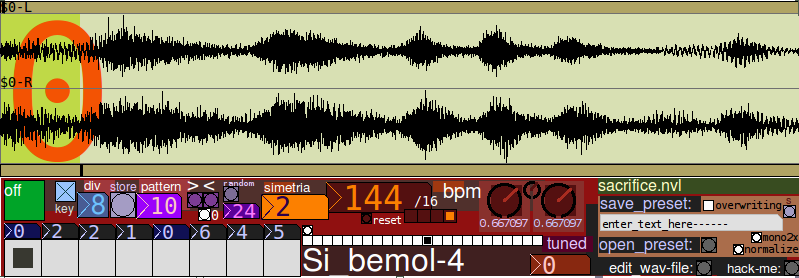
\includegraphics[scale=.6]{navalha}
\caption{navalha}
\label{navalha}
\end{figure}


\begin{quotation}

O Software como trabalho artístico – Artesanato de código 

Este projeto é um estudo para estimular uma atividade que torna-se cada vez mais evidente no universo 
do software livre e código aberto – a customização de softwares para idéias artísticas e para produção 
multimídia em geral permitindo aquele que via criar desenvolver suas idéias abstratas partindo de maneiras 
rápidas de trabalhar com código, ao invés da lógica onde o artista e visto como um usuário de interfaces ja 
prontas que ao tentar “prever aquilo que quer o usuário” também acaba impondo sua prática de uso.

Com a escolha da linguagem puredata, que possui uma comunidade extremamente produtiva e colaborativa,  
por mais que esta interface esteja apresentando uma prática fechada em uma idéia de recortes de samples e um 
certo escopo, apresenta-se também como a abertura para ser recombinada com outros códigos e idéias, colocando-se 
como uma peça a ser aberta e transformada, sendo desde o início deste projeto documentada da maneira mais detalhada 
possível para permitir tal recombinação.

Navalha é um software desenvolvido com o intuito de tornar-se um estudo de caso em desenvolvimento rápido prototipado 
em Puredata de um sistema para performances musicais com interface gráfica e sistema de gerenciamento de “presets” 
(configurações) salvos em disco rígido. Além de sua utilidade para musicos e artistas é também um detalhado estudo 
de caso de desenvolvimento em puredata, podendo ser usado como estudo para implementação de outros algoritmos e idéias.
\end{quotation} 


A segunda fase da pesquisa foi o desenvolvimento do
sistema propriamente dito, com prototipação de interface para usuário,
diversos experimentos de estúdio onde cada parte do sistema será
testada individualmente e em grupo.




\section{Glossário}
\label{glossario}


\textbf{Pitch}: Termo relativo a altura das notas, em alguns módulos da pesquisa,
o valor de pitch aparece como um símbolo da nota seguido da oitava respectiva (D4, se
referindo a nota ré da oitava central do piano). Em outros momentos o valor de pitch
se refere ao parâmetro MIDI de 0 a 127. Algumas funções convertem valores puros de frequência
em pitch.

%% acrescentar que frequência é medida numa distribuição exponencial e pitch está disposto
% numa distribuição linear.

\textbf{MIDI}: É a sigla para \textit{Musical Instrument Digital Interface} e descreve um protocolo padrão da indústria, 
definido pela primeira vez em 1982, que permite que instrumentos musicais eletrônicos 
(sintetizadores e máquinas geradoras de som), computadores e outros equipamentos eletrônicos (controladores MIDI , 
placas de som, samplers) se comuniquem e se sincronizem um com o outro. 
As principais funções MIDI incluem comunicação de mensagens de eventos sobre a notação musical,  variação de altura, 
intensidade, sinais de controle para os parâmetros (tais como volume, vibrato, panning, pistas e sinais de 
clock (para definir o tempo)) entre dois dispositivos, a fim de completar uma cadeia de sinal e produzir som 
audível a partir de uma fonte de som. Como um protocolo eletrônico, é notável pela sua adoção generalizada em 
toda a indústria da música.


\textbf{Envelope}: É a definição de como a amplitude de cada nota se comporta.
É um termo comum nas especificações de síntese sonora e é um aspecto decisivo na construção e 
definição do timbre. Normalmente se dividem as fases do
envelope sonoro em ataque, decaimento, sustentação e finalização (ADSR). Por
exemplo, o timbre de um tambor tem um ataque curto, nenhuma sustentação
e uma rápida finalização.

\textbf{Pure data (Pd)}: É uma linguagem de programação visual desenvolvida por Miller Puckette na década de 1990 
para criar música computacional interativa e obras multimídia. Enquanto que Puckette é o autor principal do programa, 
o Pd é um projeto open source que conta com uma base de desenvolvedores trabalhando em novas extensões e funcionalidades.
Ele é liberado sob uma licença similar à licença BSD. Ele roda em GNU/Linux, Mac OSX, iOS, Android e Windows. 
Versões mais antigas ainda existem para FreeBSD e IRIX. Existem diversas distribuições ou "forks" de Pd, como 
Pd Vanilla, Pd-extended, DesireData e libpd. A principal característica do Pd é a semelhança da aparência do código com
a representação formal do algoritmo implementado.


\textbf{Objetos}: São funções pré-compiladas que providem uma variedade de funções.
Os objetos no Pd são escritos em C e possuem uma maneira própria de especificar as entradas e saídas
de dados para que o objeto funcione em tempo-real conectado graficamente a outros objetos.
Ao longo do texto iremos usar uma notação como por exemplo: [objeto-teste] para
representar um objeto.

\textbf{Mensagens}: São sequências de valores, listas ou símbolos. Uma mensagem pode ser usada para
guardar dados e funciona também como um botão gráfico, podendo ser acionada com um clique de mouse.

\textbf{Caixas de número}: Normalmente são usadas para teste, manipulação e/ou vizualisação
dos dados em tempo real. Graficamente são usadas como botões de valor dinâmico.

\textbf{Símbolos}: Símbolo do tipo string.

\textbf{Comentários}: Ferramenta de documentação local dos patchs.

\textbf{Objetos gráficos}: Alguns são úteis como sliders (objetos [vsl] ou [hsl])  e botões diversos como
toogle (objeto [tgl]).

\textbf{Arrays}: Tabelas de uma dimensão que podem ser utilizados por qualquer objeto
que interprete formatos diversos, desde arquivos de áudio .wav até arquivos de 
texto puro.


\textbf{Patchs}: São programas escritos em Pd.

\textbf{Sub-patchs}: É um objeto que guarda uma porção de código encapsulado, funciona
de forma local, ou seja, restrito ao patch principal.

\textbf{Abstrações}: É um patch que funciona como um objeto normal, porém escrito em Pd e pode agir de maneira global.
Como é salvo separadamente pode ser carregado quantas vezes for preciso em diversos patchs. Formalmente na linguagem,
 uma abstração também é considerada um objeto.

\textbf{int, float}: São especificações do Pd para designar números inteiros e números decimais.

\textbf{Biblioteca} é um conjunto de objetos para determinada função.O desenvolvimento
central do Pd é nos objetos de matemática e processamento de sinal de áudio. Enquanto
que a comunidade implementou diversas bibliotecas para processamento de vídeo e sensores
de controle. 


\begin{figure}
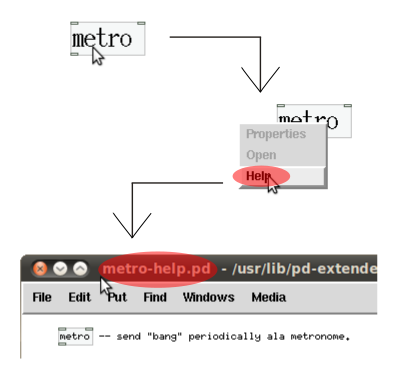
\includegraphics[scale=.6]{help}
\caption{exemplo de acesso ao manual do objeto metro}
\label{help}
\end{figure}


\textbf{Manual do objeto}: Se trata de um patch que exemplifica o uso de determinado
objeto. O próprio editor gráfico do Pd entende que um patch que tenha o nome do objeto 
acrescido de "-help" é referenciado no menu disponível com o clique direito do mouse. 
Na figura \ref{help} vemos que o objeto metro tem o manual
referenciando o patch metro-help.pd acessando um 
menu com o botão direito em cima do objeto em questão.



\textbf{Sample}: É uma amostra de áudio, que tem suas propriedades dependentes da
taxa de amostragem e resolução de bits do sistema.


\textbf{Mixer}: É a designação de um controlador de volume ou intensidade de canais separados 
e independentes.

\textbf{Loop}: Repetição literal ou alterada de trechos de samples pré-gravados ou
gravados no momento da performance.


\section{Idiomas comuns}

%% Aqui falar desses elementos mas usando abstrações de SINCOPA

O Pd é uma linguagem de programação completa, porém alguns aspectos triviais
de linguagens de programação textuais se tornam relativamente complexos e vice-versa.
Dentro do escopo dessa pesquisa é fundamental o estabelecimento de uma metodologia de
implementação de alguns idiomas comuns a todas linguagens de programação.

Mesmo dentro de uma mesma linguagem, podemos encontrar diversas maneiras
de realizar o mesmo procedimento. Nessa seção serão apresentados alguns idiomas comuns 
que ao longo da pesquisa se tornaram padrões dentro do projeto de cada
objeto de SINCOPA.
 
\subsection{Escrita em arrays}

\begin{figure}
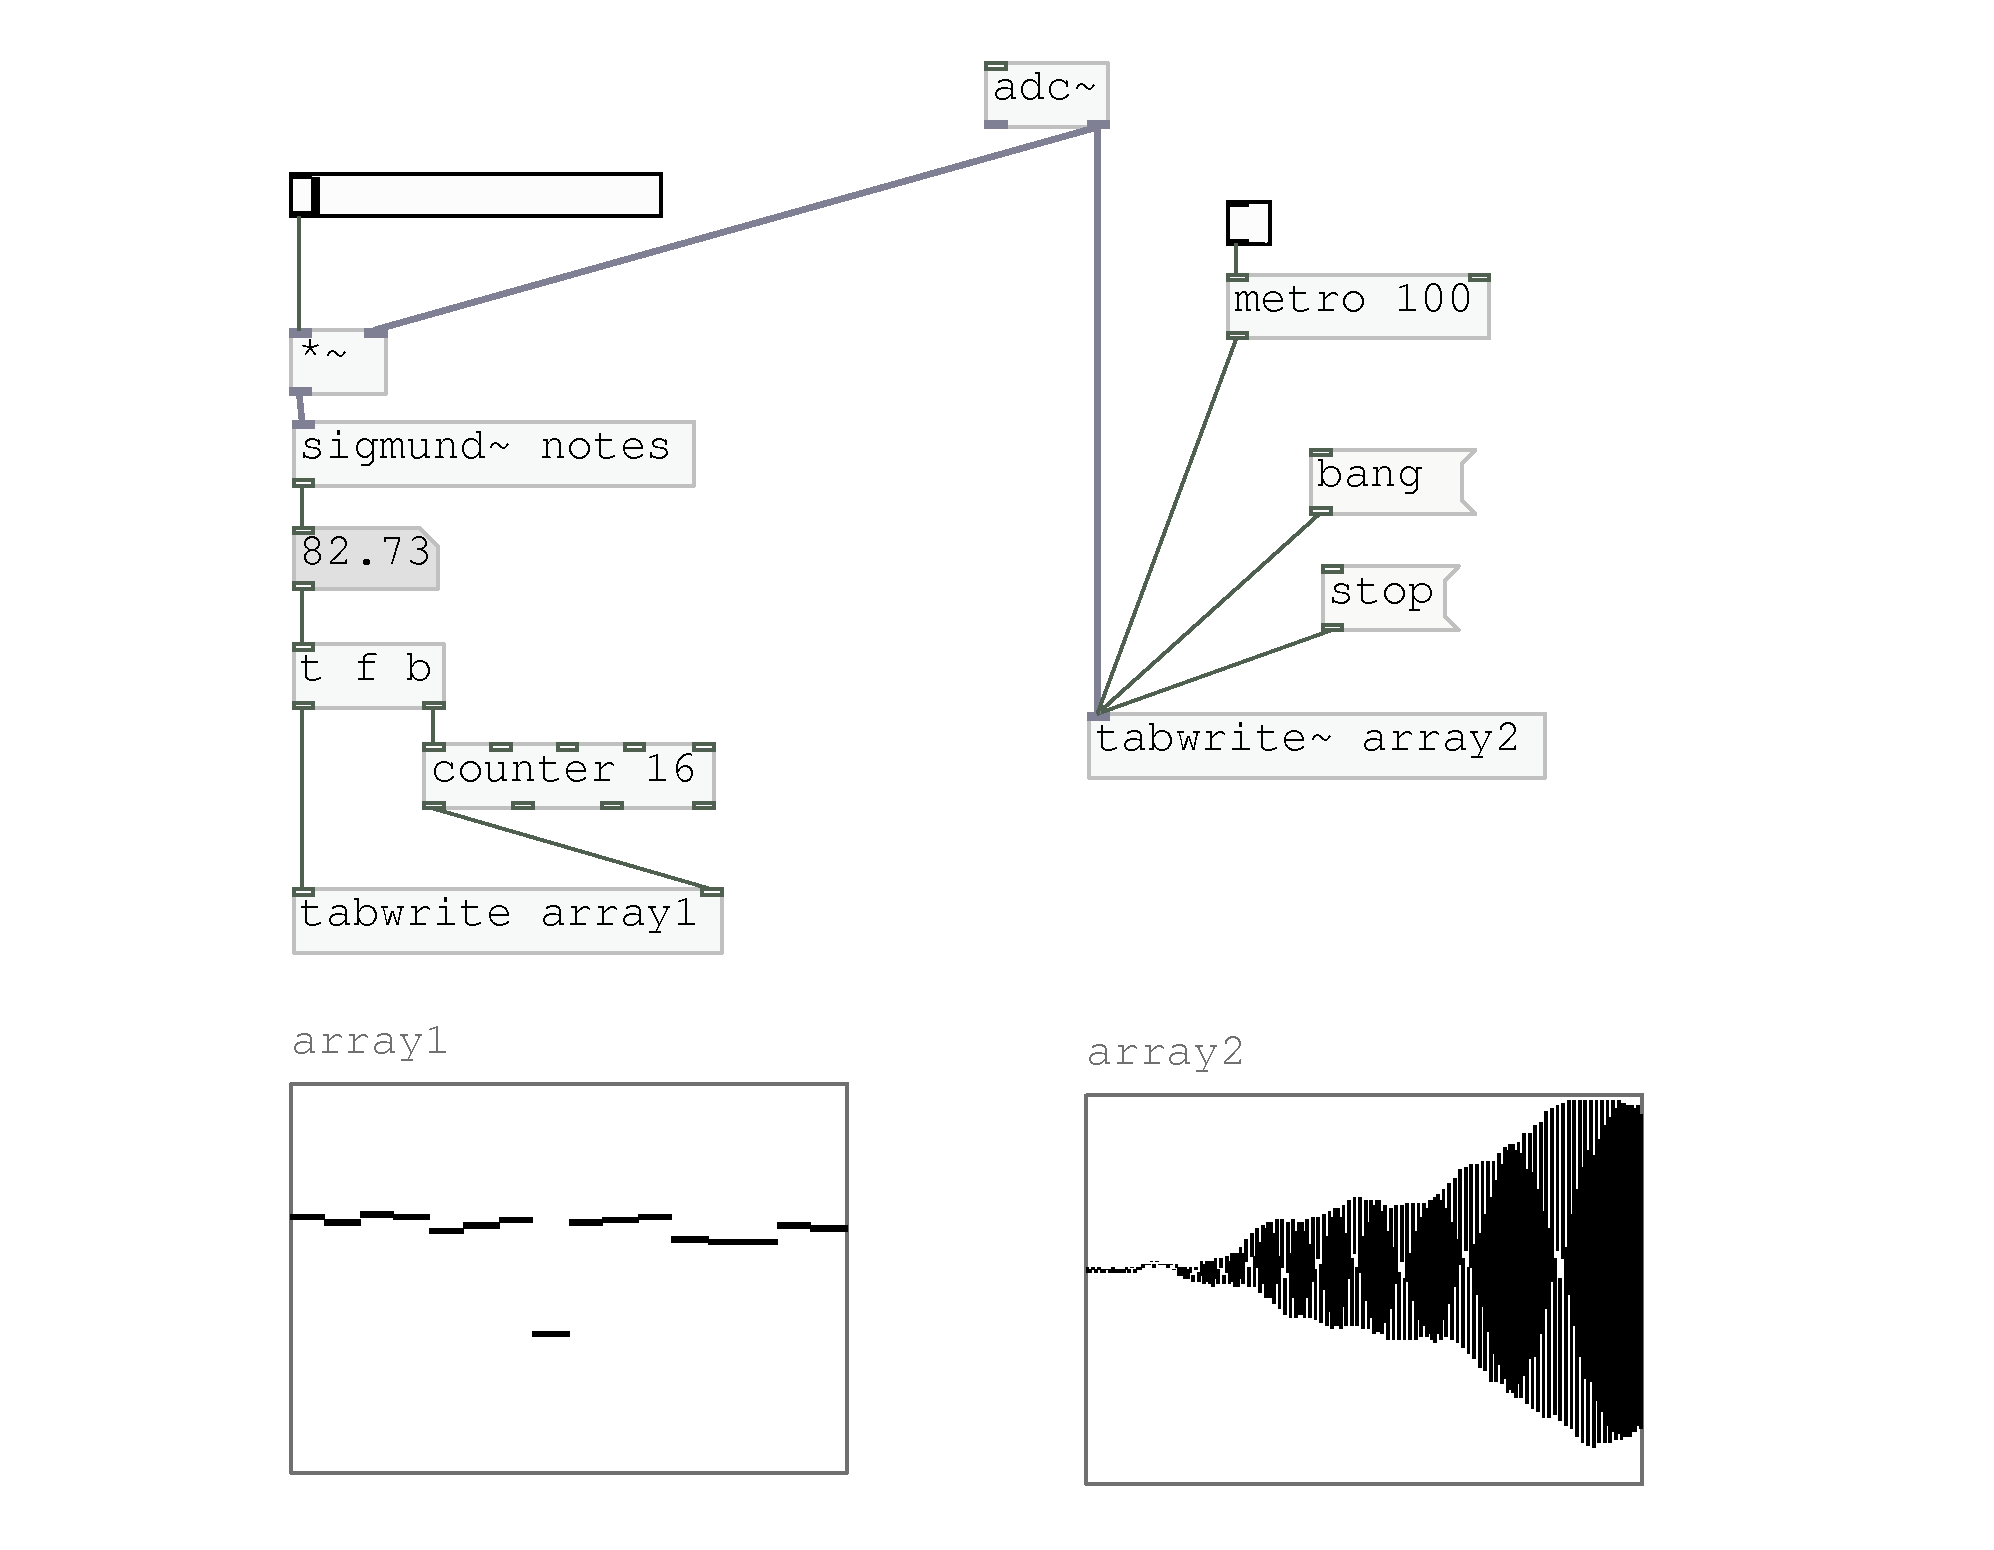
\includegraphics[scale=.6]{escrita-array}
\caption{exemplo de escrita de áudio e números em arrays}
\label{escritaarray}
\end{figure}

Na figura \ref{escritaarray} vemos as duas principais funções dos arrays
no Pd, como escrita de números "floats" ou "ints". E como tabela de escrita
de áudio, podendo ser usado com o objeto [tabwrite\texttildelow] e também
com o objeto [soundfiler] no caso de abrir um arquivo de áudio previamente
gravado em disco.


\subsection{Conexão por cabos vs [send] [receive]}

\begin{figure}
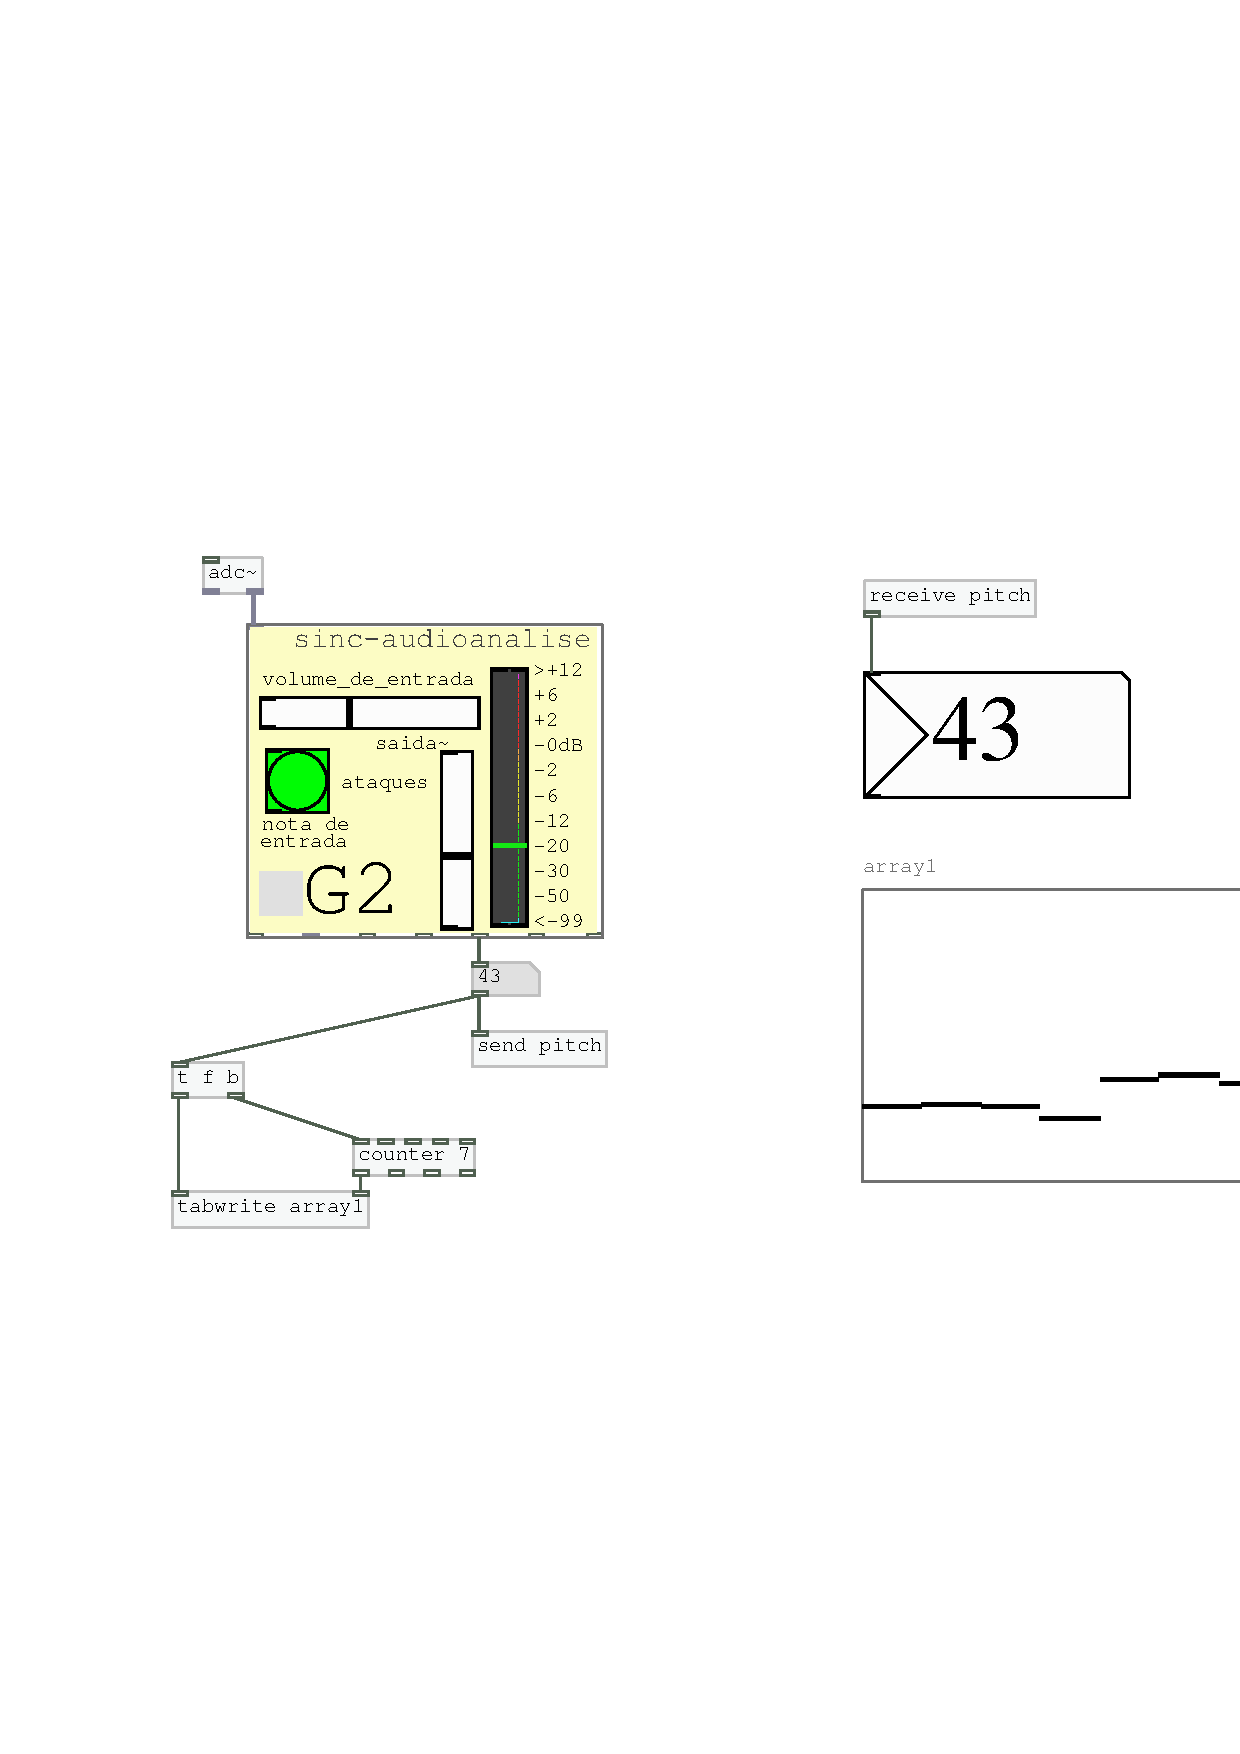
\includegraphics[scale=.6]{ex-conexoes}
\caption{conectando saídas de objetos com cabos e com [send] e [receive]}
\label{ex-conexoes}
\end{figure}



\subsection{variáveis locais vs variáveis globais}

\begin{figure}
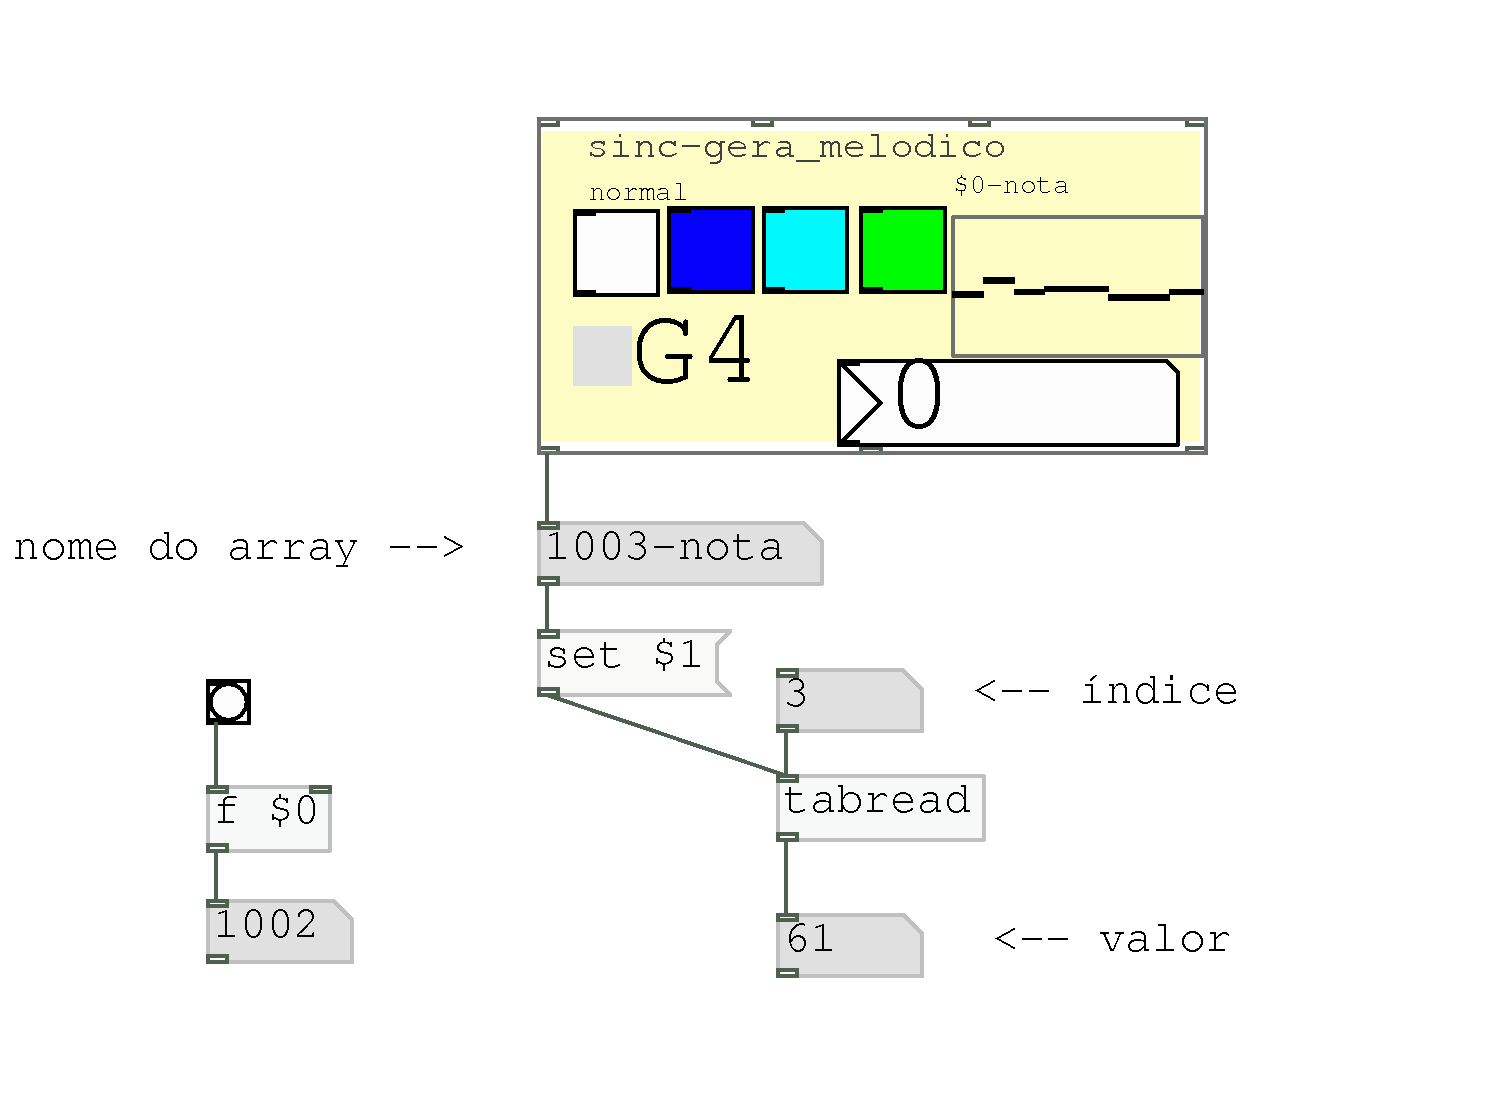
\includegraphics[scale=.6]{ex-variaveis}
\caption{[sinc-gera-melodico] enviando nome de variável local para ser lida por outros objetos}
\label{ex-variaveis}
\end{figure}

No projeto de um sistema de música interativa, lidamos com um volume grande
de variáveis locais, que precisam ser estocadas e enviadas de um objeto a outros.

No Pd é determinado o uso diferenciado entre variáveis globais e locais.
Na figura \ref{ex-variaveis} vemos um objeto de Sincopa enviando um valor de 
variável local para leitura externa por outros objetos.




\subsection{Objetos gráficos GUI's, subpatchs/abstrações e canvas}


* importância da interface gráfica ser "amigável"

* bugs e incompatibilidades em muitos objetos gráficos



\subsection{Objeto [expr] vs. sequência de objetos}

* diferença entre uma operação matemática com objetos de pd e com expr

* semelhança de expr com C

* remeter a criação de external em C no apêndice

* problema da diferença de licença da família expr para o resto do Pd


\subsection{Diferenças entre mensagens de controle e fluxo de áudio}

* uso do [switch\texttildelow]

* [line\texttildelow] como controle de volumes


\subsection{Amplificação de áudio}

* clipagem e vizualização...como "desclipar" , normalizando um array com tabletool (princípio do limiter)

\section{Ferramentas}

Nessa seção serão brevemente expostos os motivos pela escolha de determinadas ferramentas para
o desenvolvimento dessa pesquisa.


\subsection{GNU/linux}

Durante toda a pesquisa, foi usado o sistema operacional GNU/Linux.
As distribuições usadas foram Debian testing, Debian stable e Ubuntu LTS.
Muitos motivos poderiam ser listados para justificar a escolha desse sistema
operacional. Porém, gostaria de destacar a preocupação pela coerência de licenças
de uso e distribuição, entre as diversas partes que compõe a pesquisa.
O objetivo é construir programas usando componentes de software que usem as licenças GNU/GPL, ou 
BSD. O código resultante dessa pesquisa também é licenciado sob as especificações
da licença GNU/GPL.



\subsection{Git}

Git é um sistema de controle de versão distribuído, com código fonte livre e aberta, desenhado para lidar com qualquer
projeto, com rapidez e eficiência.
Uma grande vantagem é a facilidade de colaboração em desenvolvimento de código, onde outros desenvolvedores
podem clonar o repositório da pesquisa e realizarem "forks", ou desenvolvimentos paralelos. Isso cria uma situação 
onde o resultado da pesquisa, em termos de programação, se torna um elemento vivo dentro da comunidade de músicos e 
programadores interessados em computação musical e música interativa.

Além da possibilidade de fácil manutenção de repositórios de código local, muitas empresas oferecem serviços de
hospedagem gratuita de repositórios Git na internet. A escolha desse controle de versão se dá pelo estímulo a cooperação e 
continuidade dessa pesquisa para além do encerramento da tese, com a possibilidade de alguns resultados se proliferarem
em outros projetos de pesquisa.



\subsection{Jack}

JACK é um sistema para o tratamento em tempo real, áudio de baixa latência (e MIDI). 
Ele roda em GNU / Linux, Solaris, FreeBSD, OS X e Windows (e pode ser portado para outras plataformas 
POSIX-conformant). É possível conectar um número de diferentes aplicações para um dispositivo de áudio, 
bem como permitindo que eles compartilhem áudio entre si. Seus clientes podem ser executados em seus próprios 
processos (ou seja, como aplicações normais), ou podem eles podem ser executados dentro do servidor JACK 
(ou seja, como um "plugin"). JACK também tem suporte para a distribuição de processamento de áudio através de 
uma rede, tanto LANs rápido e confiável, bem como mais lento, WANs menos confiável.

\begin{figure}
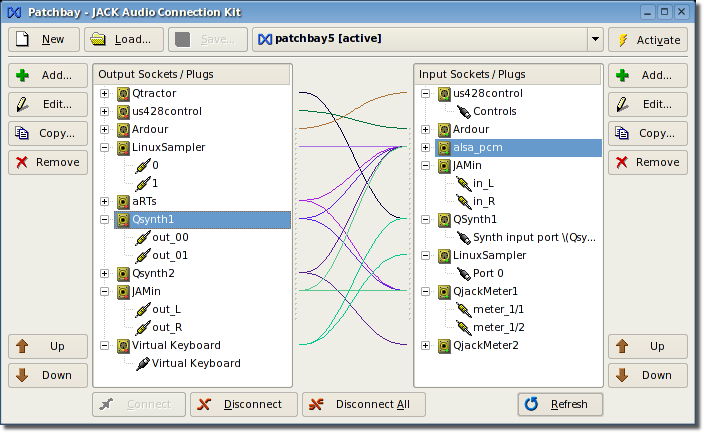
\includegraphics[scale=.7]{qjackctl}
\caption{Interface de conexão de processos do Jack}
\label{jack}
\end{figure}



\subsection{rosegarden}

Rosegarden é um programa de criação e edição musical que roda em GNU/linux.
Possui diversas funcionalidades, mas nessa pesquisa é usado como sequenciador
MIDI gráfico, que recebe mensagens MIDI em tempo-real através do Jack.

A vantagem é a possibilidade de editar graficamente o resultado do diálogo entre
o áudio do instrumento convertido em MIDI e o resultado dos algoritmos dos geradores
MIDI e harmonizadores. O Rosegarden usa dois editor gráfico em formato de piano-roll
e outro em formato de notação musical. Uma sequência MIDI editada com o Rosegarden
pode ser exportada para o formato .ly, que é o formato do Lilypond.

Lilypond é uma linguagem de marcação especializada em notação musical. Segundo
a definição do próprio projeto:

\begin{quote}
 LilyPond é um programa de gravação de música, dedicada à produção a partitura da mais alta qualidade possível. 
Ele traz a estética da música tradicional escrita para impressões de computador. LilyPond é software livre e 
parte do Projeto GNU.
\end{quote} 

O Rosegarden executa as sequências MIDI usando um servidor de arquivos soundfont.
Um arquivo SoundFont, ou "banco" SoundFont, contém uma ou mais amostras de áudio de onda (ou "amostras"),
que pode ser re-sintetizados em alturas diferentes e níveis dinâmicos. Cada forma de onda amostrada pode ser
associado a um ou mais intervalos de notas e dinâmica. De modo geral, a qualidade de um
SoundFont banco é uma função da qualidade das amostras de digitais e da associação inteligente
de amostras com as séries do campo apropriado. A qualidade da soundfont também depende do número de amostras
tomadas por um determinado intervalo de notas. 



\subsection{Pd-extended}

O Pure data(Pd), foi a linguagem escolhida para o desenvolvimento dessa pesquisa.
Existem diversas distribuições do Pd, sendo as mais utilizadas o Pd "vanilla" e o Pd-extended.
A versão "vanilla" se refere ao núcleo da linguagem mantida pelo criador Miller Puckette, e no
momento de escrita dessa tese se encontra na versão 0.43. Já o Pd-extended conta com as contribuições
da comunidade de desenvolvedores e usuários, que incluíram diversas extensões para vídeo, gráficos, rede e
novas funcionalidades para criação musical.

No atual momento, essa pesquisa depende do Pd-extended, porém, para o desenvolvimento futuro pretende-se
que as abstrações dependam, apenas da versão vanilla. A desvantagem de usar a distribuição Pd-extended é quebraa mesma 
depende de muitos outros componentes de software, tornando uma possível compatibilidade da pesquisa com sistemas
futuros um pouco mais arriscada. 


\subsection{Bibliotecas de Pd}

Além do Pd-extended, essa pesquisa, necessita de duas outras bibliotecas, sendo elas a PDMTL e DIY2 (ver anexo).

Também são usados os objetos compilados em C, desenvolvidos por William Brent:

\begin{itemize}
 \item tabletools
 \item timbreID
\end{itemize}


%\begin{figure}
%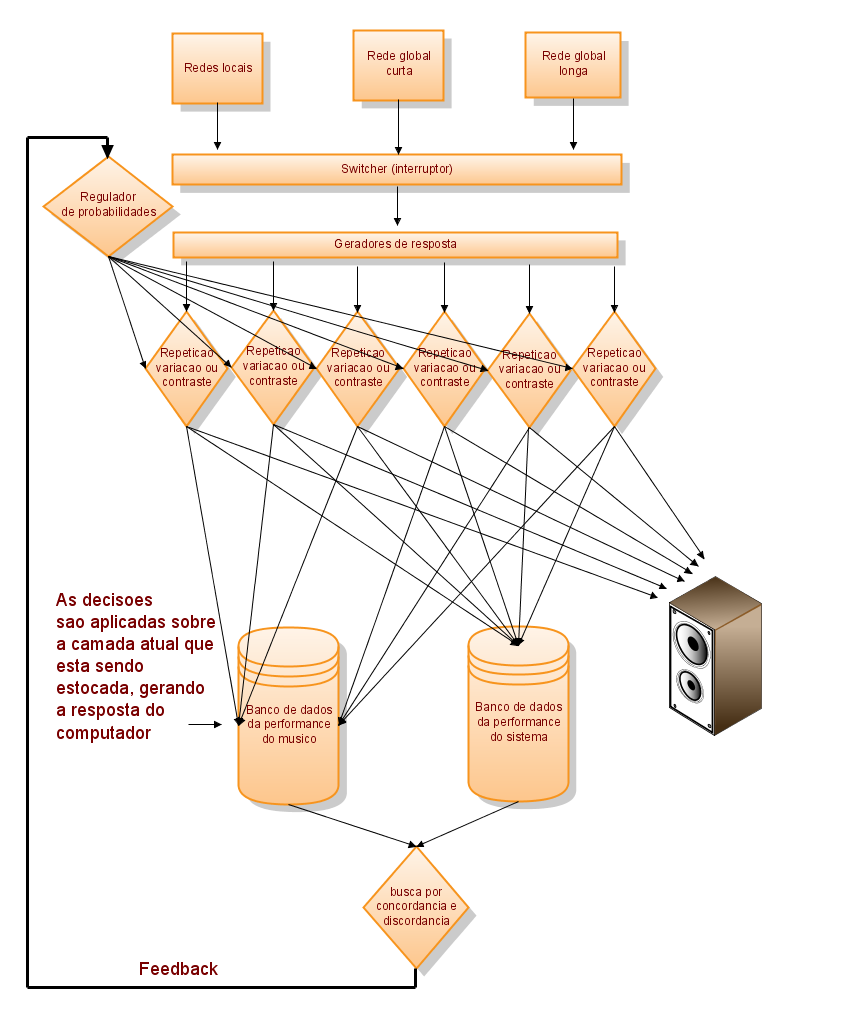
\includegraphics[scale=.6]{mecanismo}
%\caption{Mecanismo de decisões e geração de resposta}
%\label{mecanismo}
%\end{figure}



\newpage


\section{restrições/limitações}


A motivação inicial da pesquisa, foi criar um sistema interativo
para uso com instrumentos de corda pinçada como violão e guitarra.

Rapidamente se evidenciou o problema da limitação da análise de áudio
em tempo-real em relação ao aspecto polifônico desses instrumentos.
A versão atual dessa pesquisa, compreende interação com instrumentos
monofônicos.

Uma possível solução da problemática da análise polifônica é apresentada
por Puckette:

\begin{quote}
 I've been at work on a long-term project to design a rather personalized computer music instrument to try 
to bring out and confront some of the difficulties encountered by musicians trying to use computers in live 
performance. The instrument is based on a compact electric guitar (Steinberger/Gibson) with an added six-string 
separated pickup (Roland). Not finding an inexpensive and compact 6-channel preamp on the market, I designed and 
built a very crude one. This is interfaced to a computer using a multichannel PCI interface (Midiman). 
A Pd patch, running in linux, then performs a variety of interesting transformations on the six audio signals, 
and mixes them to stereo for output.

This is entirely different from standard ``guitar synthesizers" which pitch track the strings to drive synthesizers. 
Such instruments make lots of audible mistakes, and they also suffer from the added latency the comes from the pitch 
tracker. In the instrument described here, the latency of the whole affair is only that of Pd itself, about 10 
milliseconds (it's probably not hard to reduce it to 5 or 6 using real-time kernel patches but I preferred to use 
off-the-shelf linux). 
\end{quote}



\chapter{SInCoPA}
\label{chap:SInCoPA}


Na teoria musical, a síncopa é uma característica rítmica caracterizada pela execução de som em um tempo fraco, 
ou parte fraca de tempo sendo prolongado até o tempo forte, criando um deslocamento da acentuação rítmica. 
Além de SInCoPA ser a abreviação de Sistema Interativo de Composição Performance e Análise, o termo se encaixa
no sentido poético dessa pesquisa. Como uma metáfora, significando a busca de um gesto musical não determinado pela notação
ou por uma pré-configuração de software que determine de forma dominante a narrativa musical.


  Nesse capítulo serão expostas as abstrações desenvolvidas para o sistema, como também
os protótipos e programas auxiliares desenvolvidos para explicar o uso correto das 
abstrações apresentadas. O conjunto de abstrações cumpre funções básicas necessárias
a projetos de música interativa que relacionem análise de áudio e geradores musicais
baseados nos dados da análise do áudio de entrada em tempo-real.

  Foi desenvolvida uma biblioteca de funções utilitárias em forma de abstrações, 
tornando fácil seu re-uso em outros projetos. As abstrações se dividem em 7 categorias:

\begin{enumerate}
 \item Análise de áudio de entrada em tempo-real;
 \item Geradores MIDI baseados no comportamento do áudio de 
entrada, com variações de controle, indo da mímese do sinal de entrada
até um grau mais elevado de contraste rítmico e melódico;
 \item Geradores de síntese sonora, também baseados no comportamento
do áudio de entrada com diversos níveis de controle;
 \item Módulos de processamento de sinal, usados no áudio de entrada e no
áudio gerado pela comunicação MIDI;
 \item Vizualizador de notação musical do áudio de entrada e de saída;
 \item Cenários de comportamentos interativos e Mixer de volumes responsivo;
 
\end{enumerate}


Uma composição musical usando o SInCoPA, consiste na concatenação de
regras que coordenam os comportamentos das várias partes envolvidas.
Esse conjunto de regras foi denominado de ``cenário''. Na composição
de um cenário o compositor escolhe, por exemplo,  se determinado gerador 
deve ter um comportamento complementar ou contrastante  em relação a algum
parâmetro de análise.



%% testar esse novo teclado - falar sobre o controlador pedal 

%% aqui pra cada patch um formato de projeto:
%% intro + objetivo + justificativa + metodologia+ conclusão e desenvolvimento futuro


%%\subsection{Biblioteca de Utilitários}



\section{Análise de áudio}

\begin{figure}
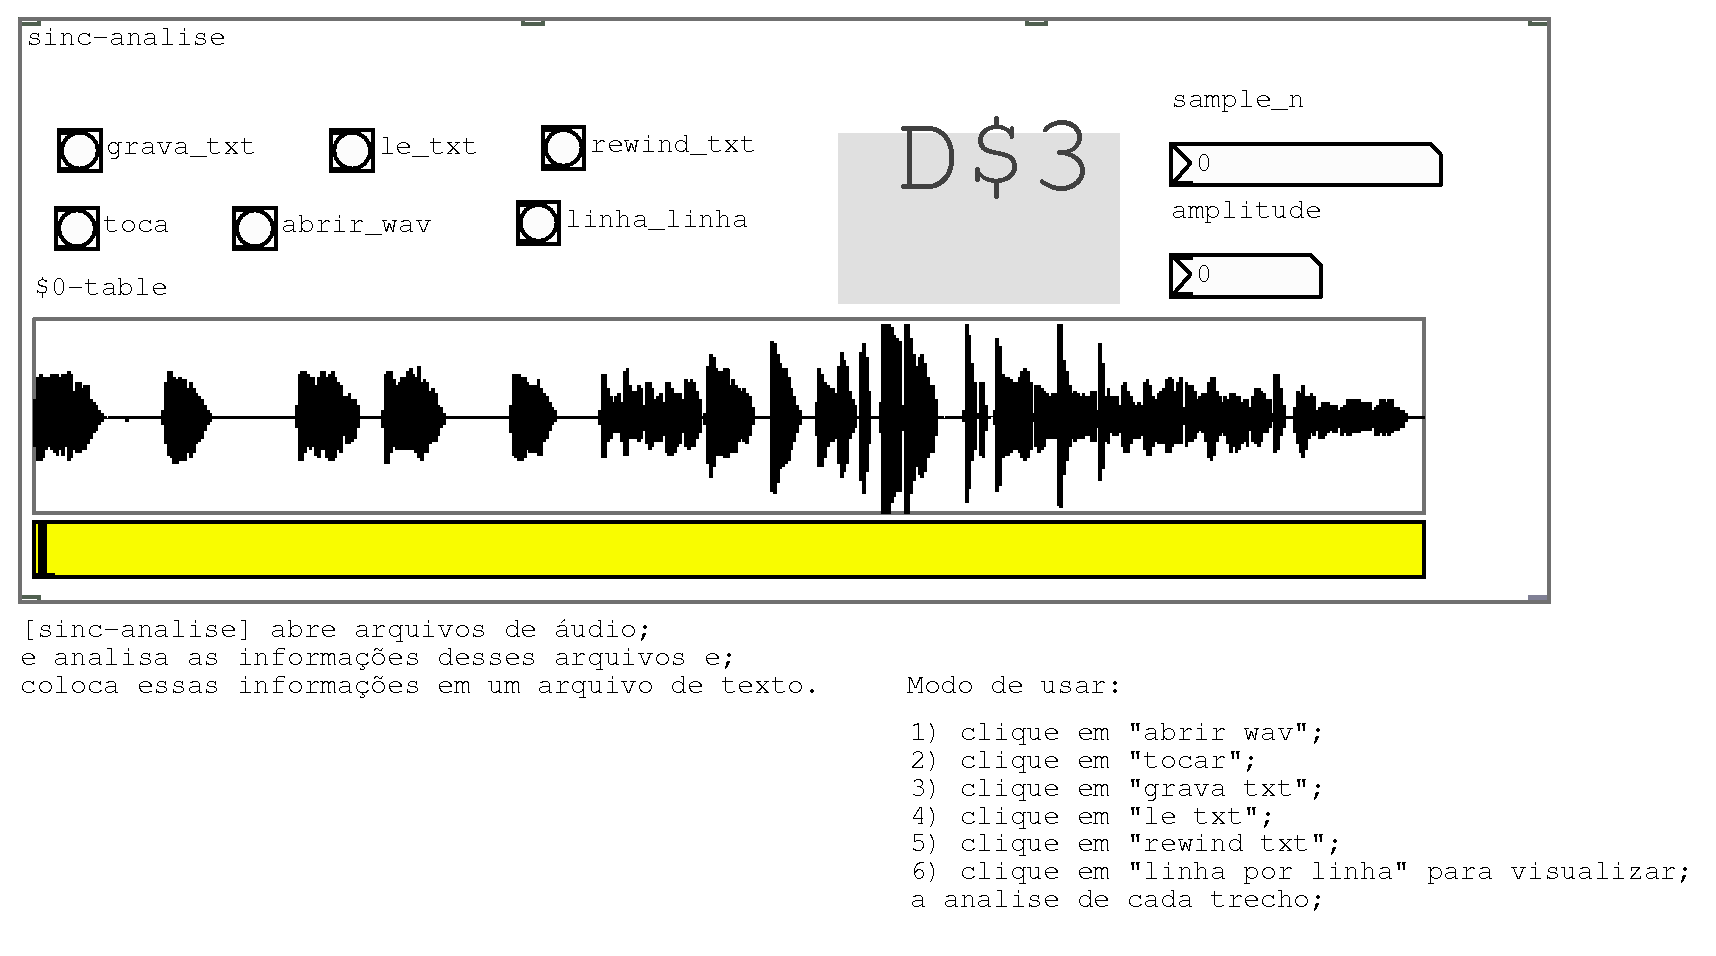
\includegraphics[scale=.7]{sinc-analise}
\caption{Objeto de análise de áudio [sinc-analise]}
\label{sinc-analise}
\end{figure}


Nessa seção serão apresentados os problemas e soluções específicos
a análise de áudio. 

É importante a flexibilização para a detecção de parâmetros musicais.
Também é importante a possibilidade de salvar os dados das análises serem
destacados nas interfaces dos objetos.

A interface gráfica dos objetos prevê vizualização em tempo-real
da atividade no módulo de análise e botões descritos para controle
de parâmetros diversos.

Um dos primeiros objetos desenevolvidos para análise é o [sinc-analise],
mostrado na figura \ref{sinc-analise} que faz análise de fundamental e amplitude
de ataque de cada nota. Esses dois parâmetros são colocados em uma lista, juntamente com a indicação
de qual sample (localização) a lista se refere e são salvos em um arquivo de texto.



\subsection{Entrada de áudio}

Um elemento importante na interface é a vizualização instantânea
do fluxo de áudio. Aqui na figura \ref{audioin} apresentamos uma solução prática e podemos
ver uma outra abordagem nas figuras \ref{fft-geral} e \ref{fft-aaray} baseada em análise FFT.

\subsubsection{Objeto [sinc-audioin]}


\begin{figure}
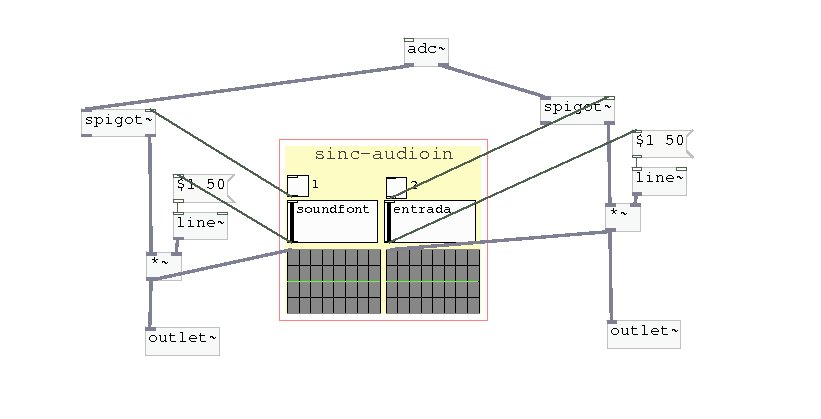
\includegraphics[scale=.55]{audioin}
\caption{Entrada de áudio [sinc-audioin]}
\label{audioin}
\end{figure}

A entrada de áudio no pd começa com o objeto  [adc\texttildelow], e sempre segue um fluxo
básico que passa por um objeto de multiplicação de sinal [*\texttildelow] que permite um
controle manual de entrada de áudio. Esse controle é necessário para ajustar 
a sensibilidade dos objetos que realizarão a análise de áudio. A abstração 
[sinc-audioin] na figura \ref{audioin} permite o roteamento e vizualização rápida 
de entrada de áudio de dois canais. No caso dos experimentos musicais envolvidos 
nessa pesquisa, foi estabelecido o canal 1 para o recebimento de áudio do programa 
rosegarden, que hospeda samplers do tipo ``soundfont''. O canal 2 é usado para 
a entrada de áudio do instrumento. É necessário um objeto que funcione como uma chave de
liga/desliga para o áudio. Para isso foi usado o objeto [spigot\texttildelow] da biblioteca
``Unauthorized'' incluída no pd-extended.
 Quando o toggle([tgl]) é acionado com clique de mouse,
ele envia o valor 1 pela saída que por sua vez está conectado na entrada fria do
[spigot\texttildelow], essa ação faz com que o áudio seja liberado pela saída do [spigot\texttildelow].
Os volumes de entrada são controlados por objetos gráficos sliders ([hsl]), que tem
a saída ligada a uma variável de parâmetro para o objeto [line\texttildelow]. Nesse caso específico
[line\texttildelow] atua no sentido de se evitar cliques no áudio quando se muda o valor de 
amplitude que entra na entrada fria do objeto [*\texttildelow]. Outro componente
opcional, que é útil em situações práticas, é um vizualizador gráfico de presença de sinal
de áudio. Em [sinc-audioin] é usado o objeto [Scope\texttildelow] da biblioteca ``cyclone'', 
incluída no pd-extended.

%% dar uma olhada no livro do Miller sobre [*~] e [line~] 

\subsection{Manipulação de amostras}


  Dentro do  contexto de laboratório de prototipação, se faz necessário emular uma entrada 
de áudio em tempo-real com a execução de trechos de áudio sampleados ou um sintetizador simples
com entrada de notas pelo teclado alfa-numérico do computador. Nesse sentido foram construídas
algumas abstrações para facilitar o processo de desenvolvimento e teste.

\subsubsection{Objeto [sinc-sample]}



\begin{figure}
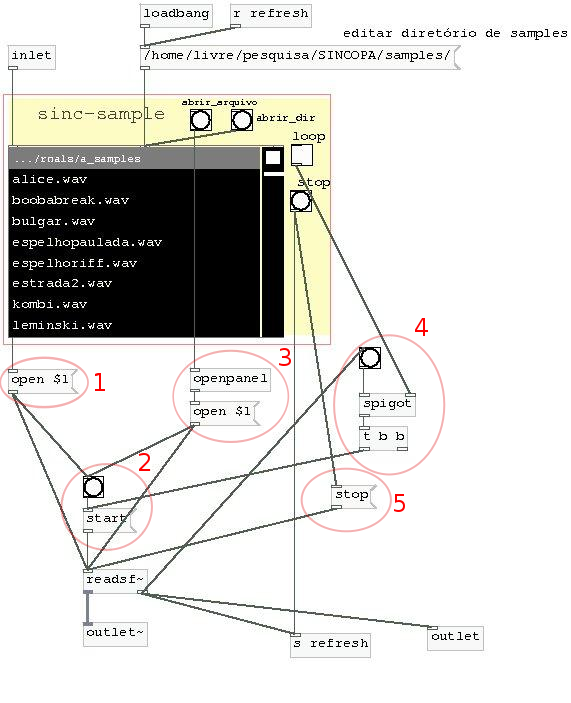
\includegraphics[scale=.5]{sinc-sample}
\caption{[sinc-sample]}
\label{[sinc-sample]}
\end{figure}



A primeira a ser desenvolvida foi a abstração [sinc-sample] mostrado na figura
\ref{[sinc-sample]}. Para essa abstração foi escolhida a abstração gráfica 
[file.browser] 
na área 1 circulada na figura \ref{[sinc-sample]} que lê os arquivos de determinado
 diretório e lista eles graficamente possibilitando que
o usuário clique no nome do arquivo escolhido, resultando em uma mensagem com a 
localização
do arquivo. Essa abstração faz parte do pacote ``pdmtl'' de abstrações de pd.
A execução do áudio é feita com o objeto [readsf\texttildelow] que precisa de três mensagens:
start, stop e localização do arquivo. O mecanismo grifado na área 2, mostra
um objeto [trigger]([t]) realizando uma tarefa em 3 fases da direita para a esquerda:
\begin{itemize}
 \item Aciona a mensagem com o caminho do arquivo a ser tocado
 \item Aciona a mensagem ``start''
 \item Recarrega a mensagem que atualiza o diretório a ser lido por [file.browser]
\end{itemize}

Outro aspecto dessa abstração é a possibilidade de tocar um arquivo de áudio em loop.
Na área circulada 4 temos um [spigot] que atua como interruptor de um bang enviado pela
saída direita de [readsf\texttildelow], que por sua vez é enviado quando [readsf\texttildelow] 
acaba de ler o arquivo
inteiro. Se o toggle que está conectado com o [spigot] da área 4 estiver ligado, ele permite
que o bang enviado ao final da leitura seja roteado para outro objeto trigger que aciona as 
duas primeiras fases descritas acima, realizando uma leitura contínua do arquivo de áudio
escolhido.



\subsection{Análise melódica}


Existem diversos problemas de pesquisa relacionados com a
análise melódica como por exemplo:

\begin{itemize}
 \item Detecção de notas;
 \item Estimativa de nota;
 \item Conversão de fluxo de áudio em dados semânticos (MIDI);
 \item Permeabilidade melódica;
 \item Análise de contorno e direcionamento melódico;
\end{itemize}




\subsubsection{Objeto [sinc-audioanalise]}

Um dos fatores mais importantes para a prática de análise melódica
em tempo real é a flexibilidade de refinamento dos parâmetros
de análise. Esses parâmetros devem estar ao alcance rápido e documentados
e sinalizados na interface.

O objetivo é reunir num só módulo, a detecção de ataques de notas 
(baseado no objeto [bonk\texttildelow]) com a análise de frequências
baseada no objeto [sigmund\texttildelow]. Ligando o resultado das 
análises com objetos MIDI.

Nessa abstração procurou-se desenvolver uma interface que facilite
a rápida prototipação e flexibilidade de parâmetros que podem
se adaptar facilmente para diferentes fontes sonoras.

\begin{figure}
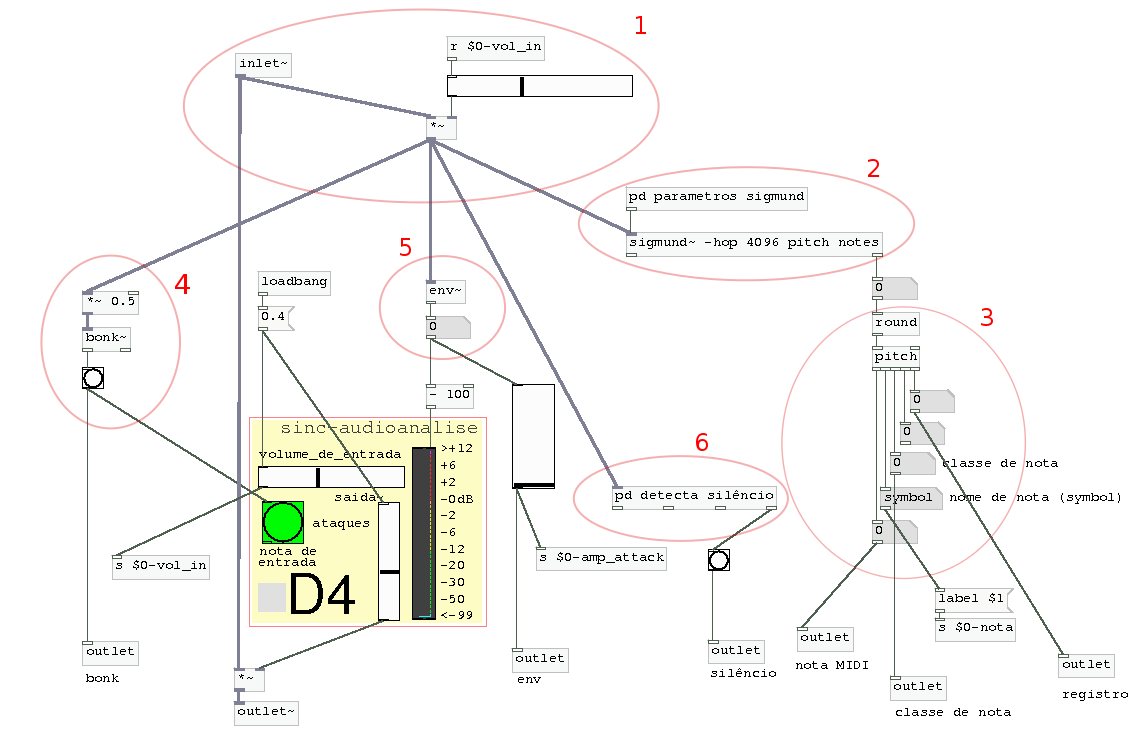
\includegraphics[scale=.4]{sinc-audioanalise}
\caption{[sinc-audioanalise]}
\label{[sinc-audioanalise]}
\end{figure}

Como podemos ver na área 1 da figura \ref{[sinc-audioanalise]},
temos o controle de um slider vertical\footnote{objeto [hslider]}
controlando a amplitude geral do áudio de entrada. Esse controle
é muito importante em situações em que se tem variações de amplificação
entre ensaios e performance.

%%Área 1: explicação da amplificação de volume de entrada/volume de saída

\begin{figure}
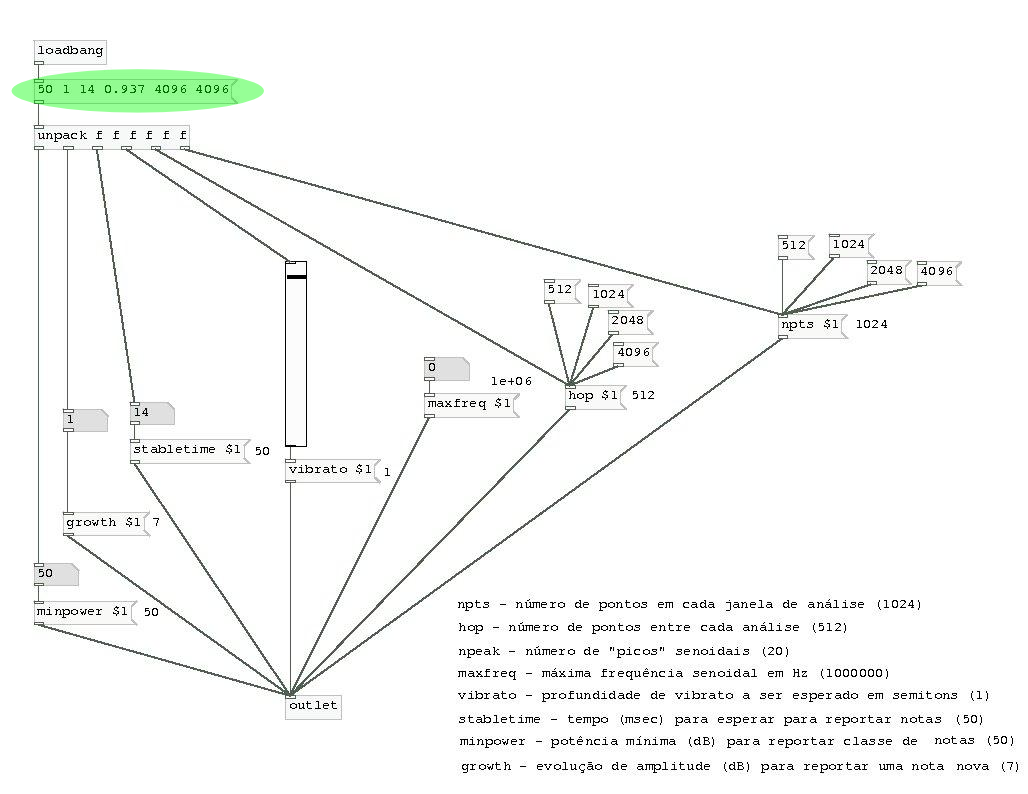
\includegraphics[scale=.5]{sinc-audioanalise-param}
\caption{sub-patch que controla as configurações de [sigmund\texttildelow]}
\label{[sinc-audioanalise-param]}
\end{figure}


Na área 2 aparece um subpatch que pode ser visto na figura
\ref{[sinc-audioanalise-param]}. Nesse subpatch podemos ver 
a organização dos parâmetros do objeto [sigmund\texttildelow].

O objeto [sigmund\texttildelow] faz análise de áudio no domínio da 
frequência e detecção de notas. Os parâmetros podem ser re-definidos
em tempo-real através dos argumentos de criação do objeto ou através
de mensagens como é o caso aqui.


Segundo a documentação no próprio manual do objeto:

\begin{quote}
 Sigmund\texttildelow analyzes an incoming sound into sinusoidal
components, which may be reported individually or combined to
form a pitch estimate. Possible outputs are specified as creation
arguments:

\begin{itemize}
 \item pitch - output continuously
 \item notes - output pitch at the beginning of notes
 \item env - output amplitude continuously
 \item peaks - output all sinusoidal peaks in order of amplitude
 \item tracks - output sinusoidal peaks organized into tracks
\end{itemize}
Parameters you may set (in cretaion arguments or messages):

\begin{itemize}
 \item npts - number of points in each analysis window (1024)
 \item hop - number of points between each analysis (512)
 \item npeak - number of sinusoidal peaks (20)
 \item maxfreak - maximum sinusoid frequency in Hz. (1000000)
 \item vibrato - depth of vibrato to expect in 1/2 tones (1)
 \item stabletime - time (msec) to wait to report notes (50)
 \item minpower - minimum power (dB) to report a pitch (50)
 \item growth - growth (dB) to repor a new note (7) 
\end{itemize}
The npts and hop parameters are in samples. and are powers of two.
\end{quote} 


\begin{figure}
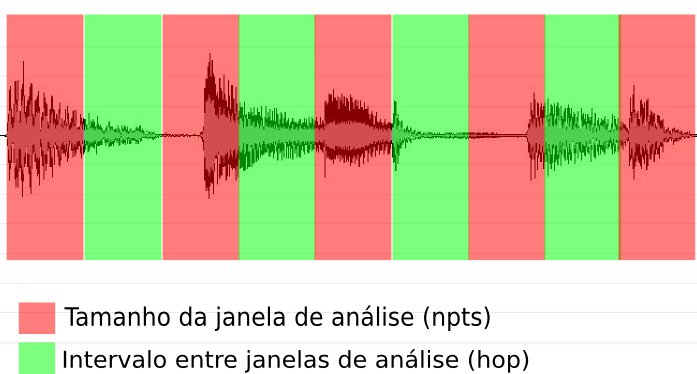
\includegraphics[scale=.7]{sigmund}
\caption{Tamanho de janela de análise (npts)}
\label{janela-analise}
\end{figure}


Nesse caso optou-se por pré-inicializar [sigmund\texttildelow] com as
opções : "-hop 4096 pitch notes" . Através de testes empíricos preferiu-se
usar apenas a saída de "notes" por apresentar uma saída mais precisa para notas 
musicais. A mensagem em destaque na figura \ref{[sinc-audioanalise-param]} representa
a inicialização dos valores de todos parâmetros de [sigmund\texttildelow].

Os principais parâmetros definem o tamanho da janela de análise.
Nesse caso "npts" e "hop" tem uma relação direta
por se tratar do tamanho da janela de análise e o espaço
entre as janelas em samples como pode ser visto na figura \ref{janela-analise}.



%%Área 2: explicação do sigmund~ - ver livro Miller + help do sigmund~


\begin{figure}
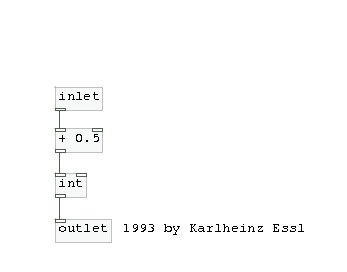
\includegraphics[scale=.5]{round}
\caption{[round]}
\label{round}
\end{figure}


Na área 3 vemos o objeto [round], presente na biblioteca RTC, responsável
por arredondar o valor de entrada para cima. O arredondamento é feito com
a soma de 0.5 e transformação do número do tipo float para tipo inteiro ([int]),
como pode ser visto na figura \ref{round}.


\begin{figure}
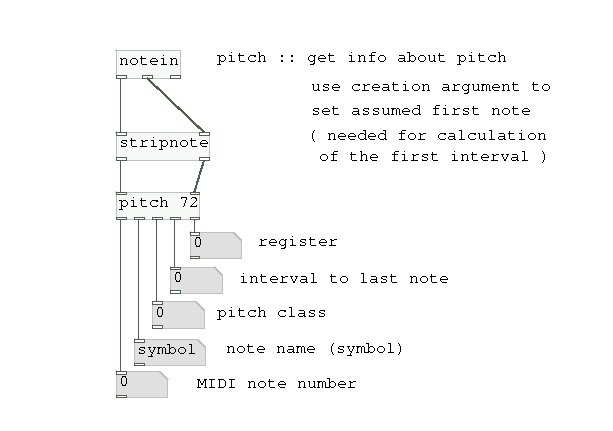
\includegraphics[scale=.5]{pitch}
\caption{[pitch]}
\label{pitch}
\end{figure}


\begin{figure}
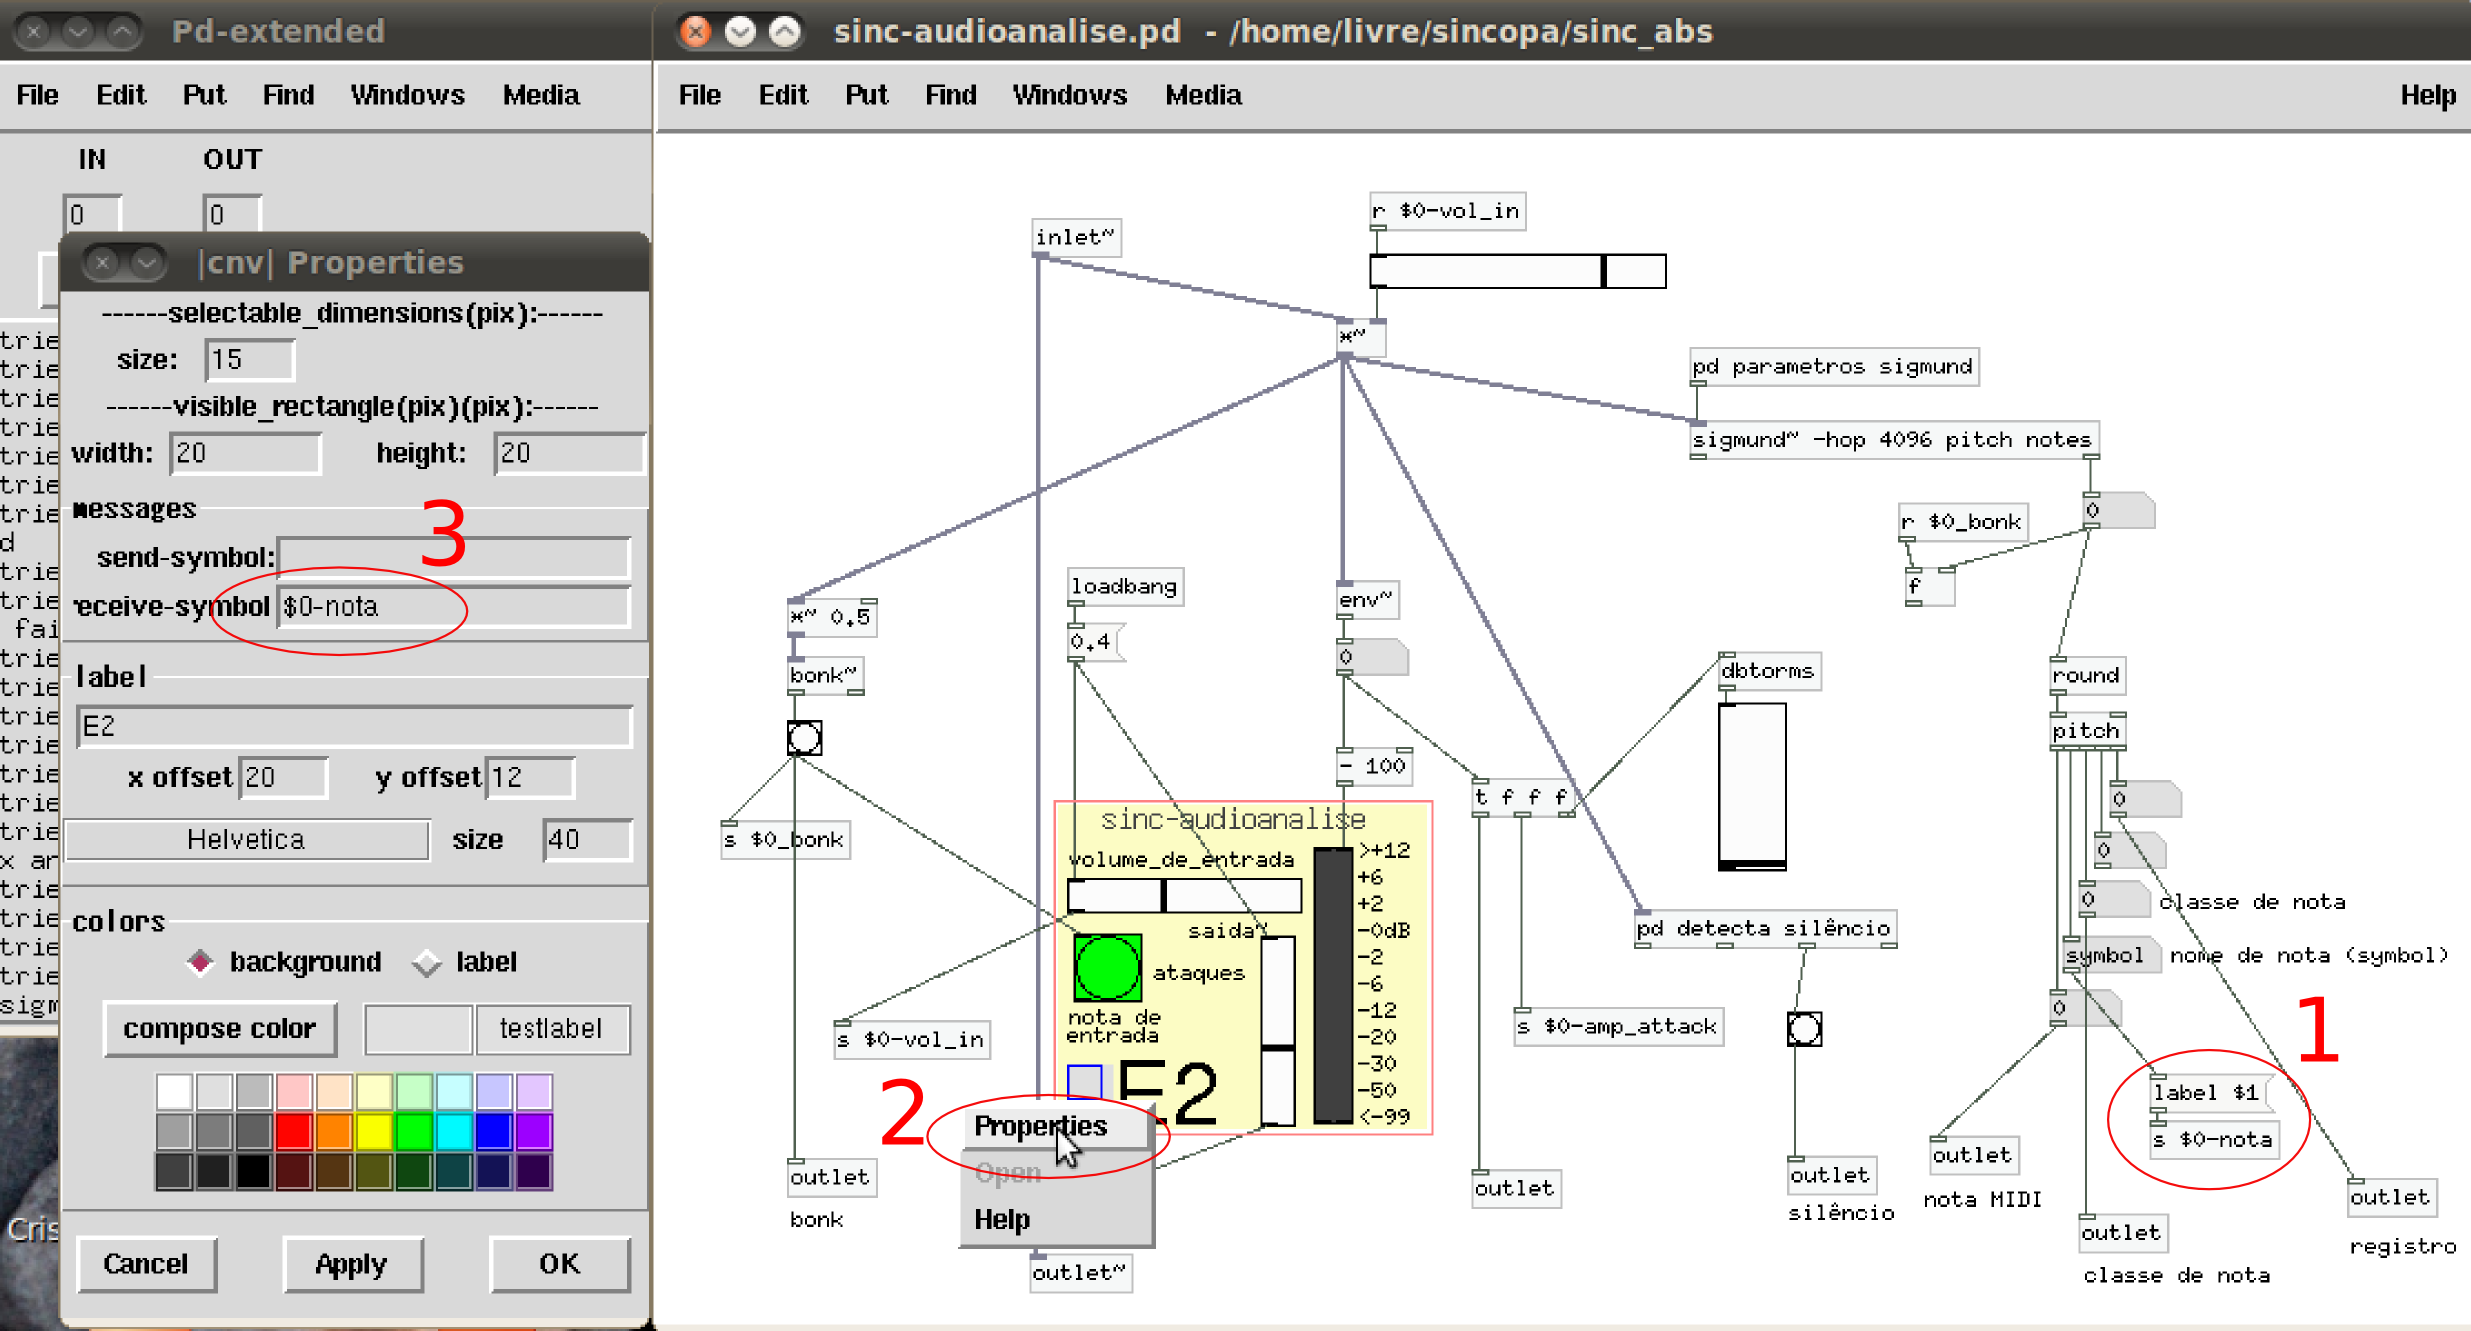
\includegraphics[scale=.5]{canvas-edit}
\caption{editando objeto canvas ([cnv])}
\label{canvas-edit}
\end{figure}


O objeto [pitch] pertence a biblioteca maxlib, distribuída junto com o 
pd-extended e sua funcionalidade pode ser vista no próprio help do objeto na 
figura \ref{pitch}. A interface gráfica de [sinc-audioanalise] mostra o pitch
da nota detectada em tempo-real. A vizualização é feita com o objeto canvas ([cnv]).
A segunda saída do objeto [pitch] retorna um símbolo com a cifra e oitava
da nota. Esse símbolo é enviado para o canvas com o método "label" através
da variável \$0-nota. O objeto canvas aceita variáveis enviadas com o objeto [send],
editando as propriedades do canvas (ver figura \ref{canvas-edit}). A vizualização em tempo-real
é indispensável para calibrar a análise de áudio.


%%Área 3: explicação de round e pitch + plotar cifra no canvas


Na área 4 vemos o objeto [bonk\texttildelow], desenvolvido para
detectar ataques de notas. Segundo Puckette:

%% biblio: Miller (Real-time audio analysis tools for Pd and MSP) - 98

\begin{quotation}
 The bonk object does a bounded-Q fillterbank of an incoming sound and
can either output the raw analysis or detect onsets
which can then be compared to a collection of known
spectral templates in order to guess which of several
possible kinds of attack has occurred.

The fiddle and bonk objects are low tech; the
algorithms would be easy to re-code in another lan-
guage or for other environments from the ones consid-
ered here. Our main concern is to get predictable and
acceptable behavior using easy-to-understand tech-
niques which won't place an unacceptable computa-
tional load on a late-model computer.
\end{quotation}

\begin{figure}
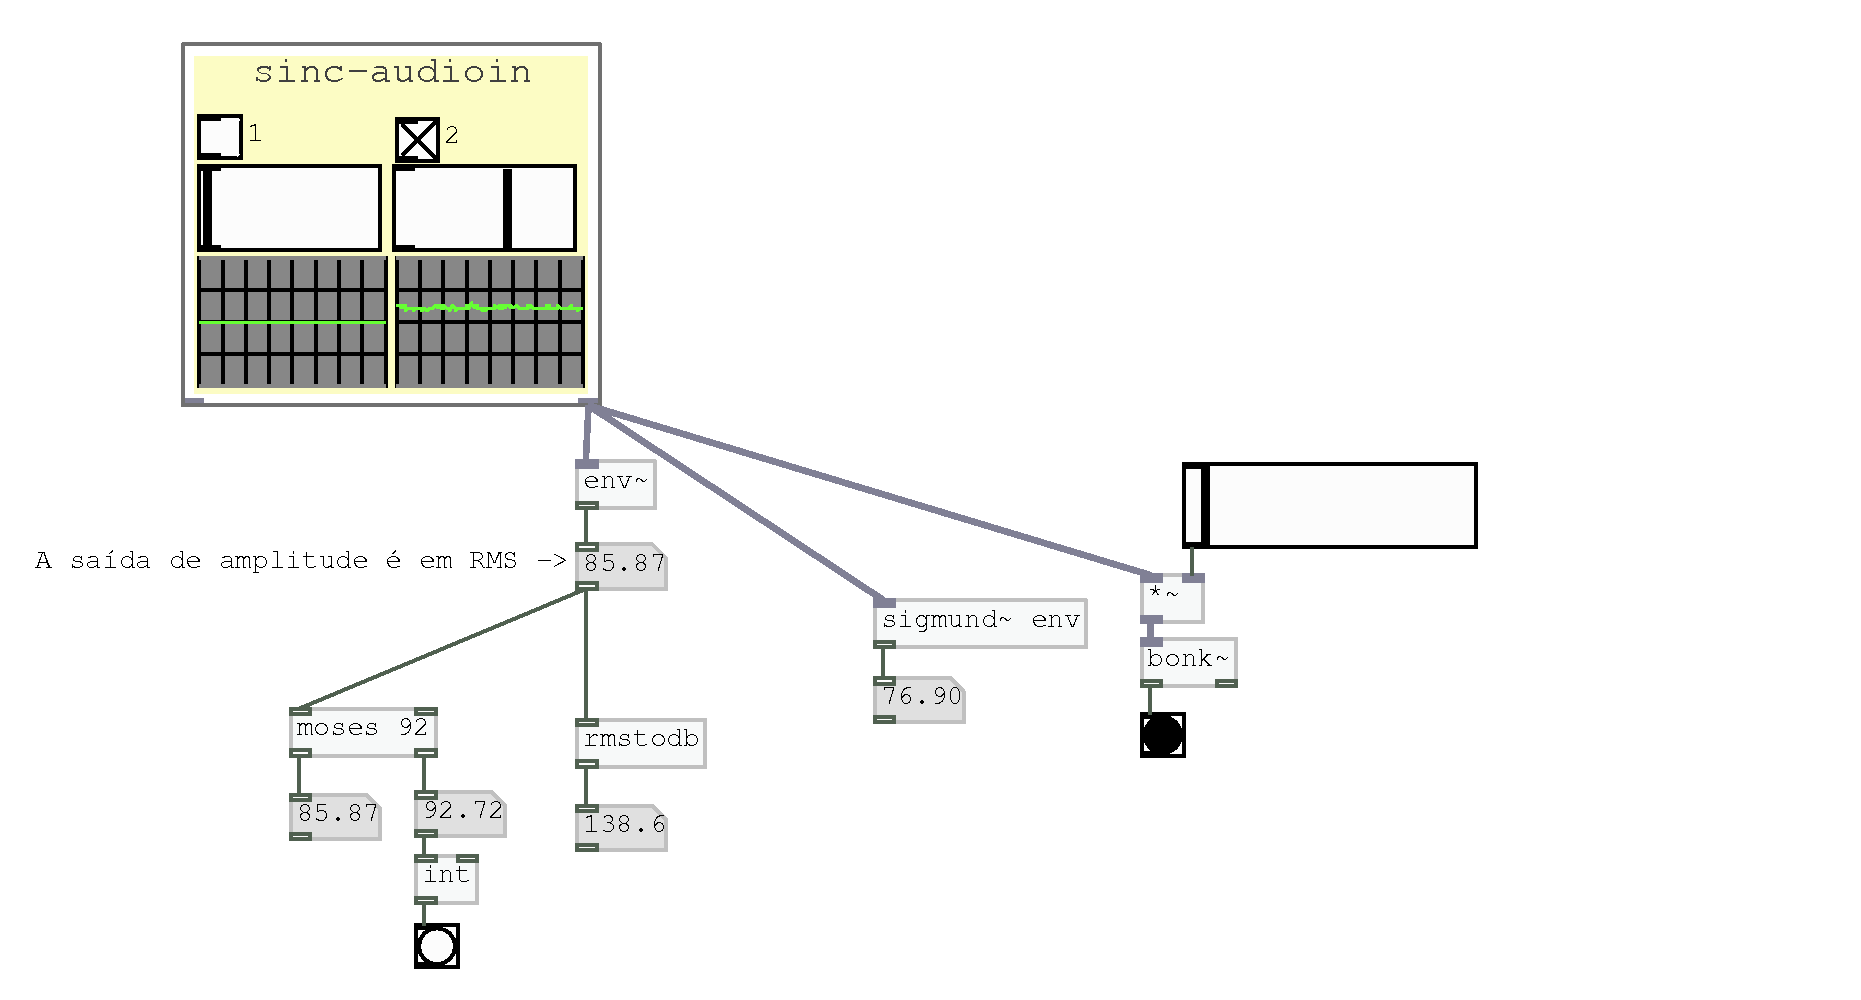
\includegraphics[scale=.5]{bonks}
\caption{Métodos de análise de amplitude}
\label{bonks} 
\end{figure}


No Pd, outros objetos possibilitam a análise da amplitude,
na figura \ref{bonks} vemos 3 métodos. O objeto [env\texttildelow]
retorna o valor de amplitude de um sinal em RMS. O objeto
[sigmund\texttildelow] pode mapear a amplitude com a opção
"env".


Ainda Puckette, aponta as vantagens de usar [bonk\texttildelow]
em vez de outros métodos.

\begin{quotation}
 
The most satisfying application of this analysis is in
detecting percussive attacks. The most popular way
of doing this is to use an envelope follower and look
for rapid rises in follower output; but any kind of
ringing can set o trains of unwanted attacks, or op-
positely, can mask true attacks. The analysis used by
bonk can often detect new attacks which appear as
sharp relative changes in the spectrum without any
accompanying large change in the overall power; con-
versely, ringing instruments don't often give rapidly
changing spectra and hence don't attract bonk's at-
tention.
\end{quotation}

A biblioteca Aubio de Paul Brossier também contém um objeto
especializado em detectar ataques de áudio [aubioonset\texttildelow].


%%Área 4: explicação do bonk~

Na área 5 vemos o objeto [env\texttildelow]. Esse objeto recebe um sinal de áudio
e retorna a amplitude RMS em decibéis (com o valor 1 normalizado para 100 dB).
A saída tem o limite inferior em zero. O algoritmo de análise interna de [env\texttildelow]
usa uma janela de análise do tipo "Hanning" (raised cosine). Uma boa aplicação de 
[env\texttildelow] é enviar o resultado da saída para o objeto [dbtorms] que transforma
os valores em decibéis em uma escala linear, que é uma distribuição melhor para vizualização
gráfica da variação de amplitude.






\begin{figure}
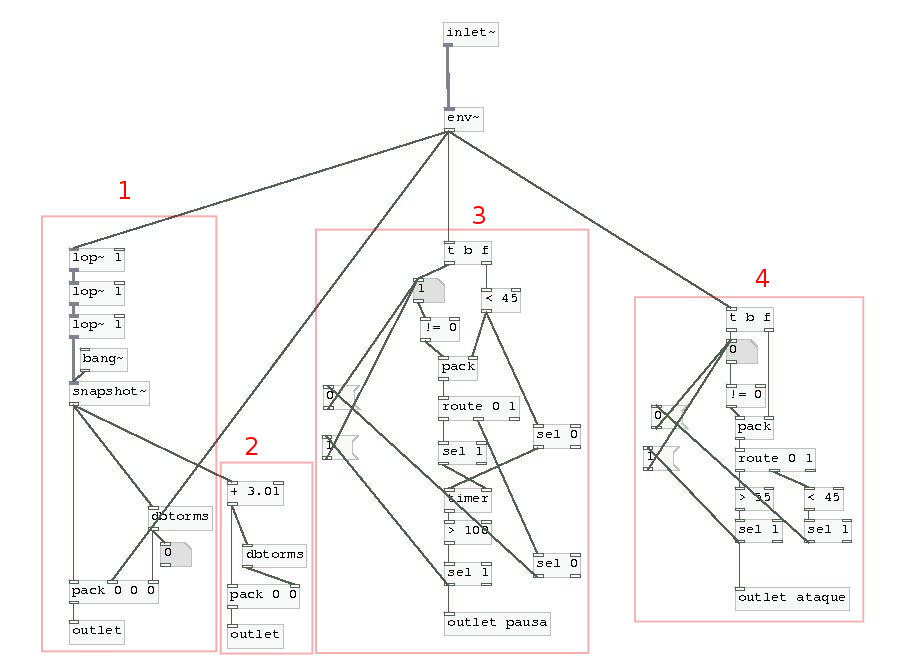
\includegraphics[scale=.5]{sinc-audioanalise-detecta}
\caption{sub-patch que detecta silêncio no áudio de entrada}
\label{[sinc-audioanalise-detecta]}
\end{figure}




Na área 6 vemos um subpatch responsável por detectar
silêncio. Na figura \ref{[sinc-audioanalise-detecta]}


Nesse sub-patch vemos 4 sub-áreas. Nessa implementação
está sendo usada apenas a terceira saída que é a saída do
módulo de detecção de silêncio. O módulo da sub-área 3
basicamente compara as amplitudes que recebe com relação ao tempo.
Nesse algoritmo, se a amplitude de entrada for menor que 45 dB durante
mais de 100 milisegundos um silêncio é detectado.



\subsection{Análise rítmica}

Se considerarmos que um evento sonoro pode ser descrito por um espaço multidimensional
onde cada parâmetro seria uma dimensão (notas, registros, timbre, etc..), podemos
imaginar o ritmo como uma outra multidimensão paralela e sincronizada com as outras.
O aspecto rítmico de um evento sonoro pode ser descrito por:
\begin{itemize}
 \item relações de durações entre ataques de notas;
\item relações de acento (amplitude) entre ataques de notas;
\item densidade de eventos em recortes de tempo;
\item descrição de índices de estabilidade em diferentes recortes temporais;
\end{itemize}

Todos esses níveis se entrecruzam para formar um cenário que pode explicar mais detalhadamente
os elementos rítmicos de um evento sonoro. O objetivo dessa seção é apresentar o desenvolvimento de
ferramentas para a análise das múltiplas camadas de descrição do ritmo.


% Aqui apresentar exemplos com formas de onda em arrays e mostrando na figura
% onde é mais denso, onde é mais instável e hierarquia de intensidade em trechos.
% 
% Mostrar também trechos maiores com índices de estabilidade.



\subsubsection{Objeto [sinc-calc-ritmo]}

Uma das questões perseguidas é o fato do sistema ter conhecimento do atual nível de 
estabilidade rítmica. Isso pode ser alcançado por uma relação que considere variações
de pulso e alternância e variações de padrões rítmicos de tamanhos diferentes.

\begin{figure}
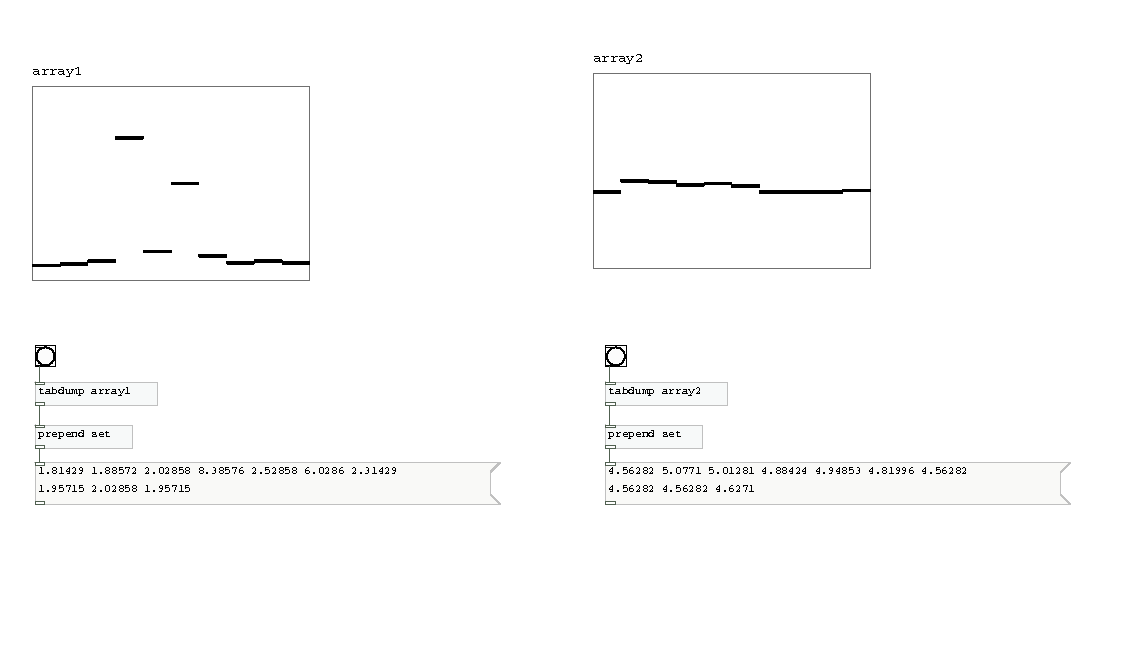
\includegraphics[scale=.6]{prot5a}
\caption{análise de estabilidade rítmica}
\label{prot5a}
\end{figure} 

Na \ref{prot5a} é mostrado dois arrays, idealmente esses arrays representam tabelas
de probabilidades de padrões rítmicos, onde cada elemento no array representa um
padrão diferente e quanto mais alto significa que teve mais ocorrẽncias.
Por exemplo, cada vez que um determinado padrão de 4 valores de duração é tocado, 
o índice na tabela correspondente a aquele padrão é incrementado. O objetivo ideal
é um mecanismo que possa retornar uma resposta do tipo:
``o array1 é mais estável que o array2''. Apenas olhando fica fácil de identificarmos
no array1 que os padrões 3 e 5 tem mais probabilidade de ocorrer pelo seu histórico,
contribuindo assim para uma sensação de estabilidade rítmica. Enquanto que o array2,
tem probabilidades próximas de quase todos padrões criando uma sensação de imprevisibilidade
e fragmentação.



No patch da \ref{[sinc-calc-ritmo]} é apresentado um método de classificação de estabilidade
de sequência de pulsos. Primeiro são calculadas as distâncias entre cada ataque
sonoro, depois filtrado em [pd filter-range] e colocado em uma tabela dinâmica em
[pd last-x]. O tamanho da tabela sempre pode ser redimensionado em tempo-real através
da variável \textit{0-buffer-size} então é calculado ao mesmo tempo a média geométrica
e a média aritmética e os resultados são executados na expressão definida por uma
divisão da média geométrica pela média aritmética. %% isso poderia ser definido em notação matemática :)
Ao resultado dessa divisão é aplicado um filtro com [moses] onde se pode calibrar
a sensibilidade do valor do índice final.


\begin{figure}
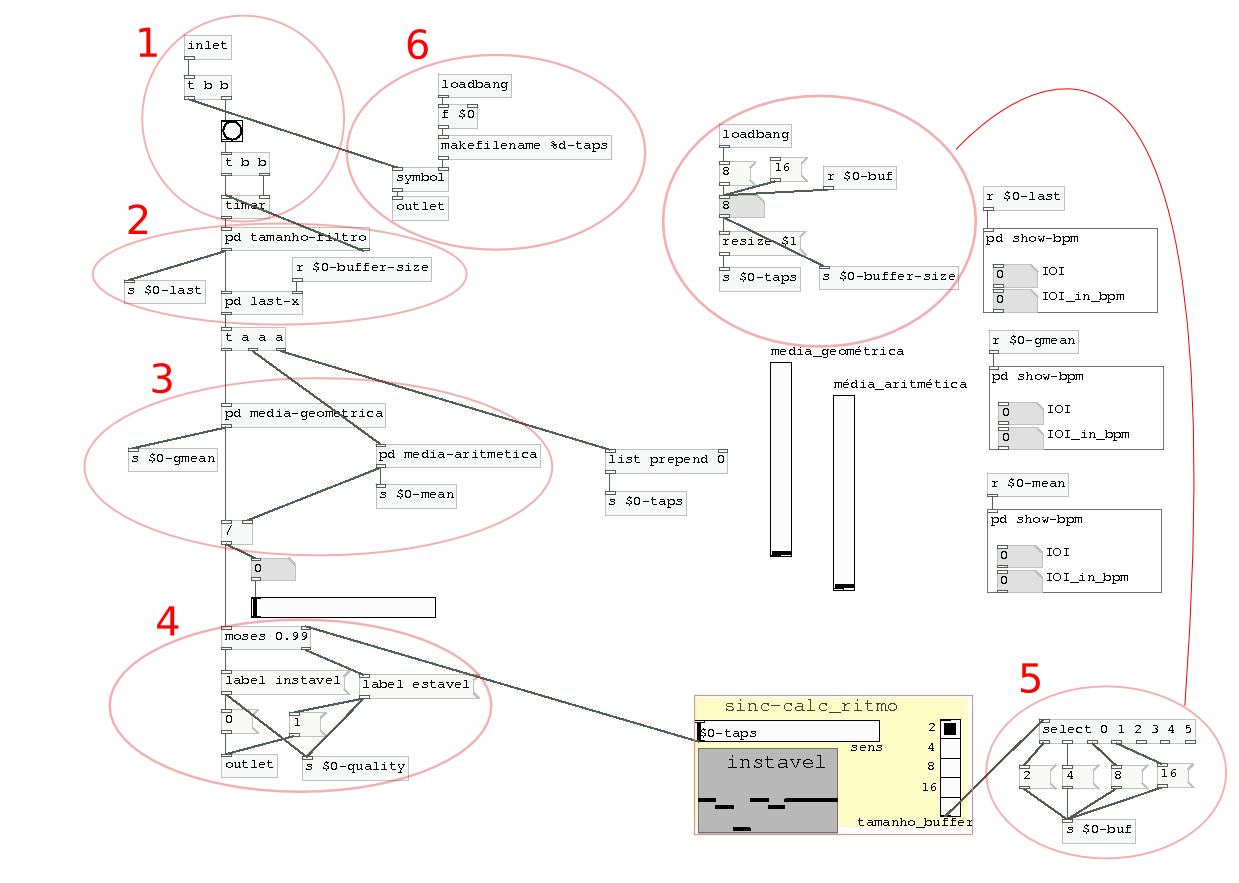
\includegraphics[scale=.5]{sinc-calc-ritmo}
\caption{análise de estabilidade rítmica}
\label{[sinc-calc-ritmo]}
\end{figure}

\begin{figure}
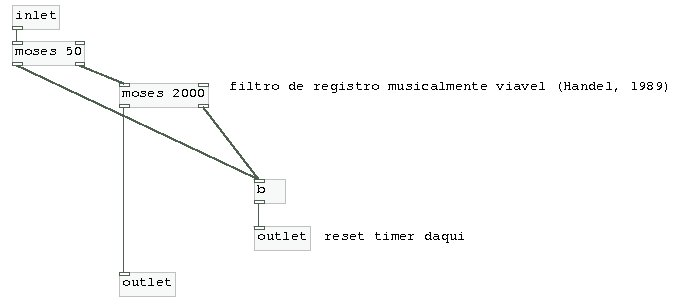
\includegraphics[scale=.5]{sinc-calc-ritmo1}
\caption{filtro de registro de durações}
\label{[sinc-calc-ritmo1]}
\end{figure}

\begin{figure}
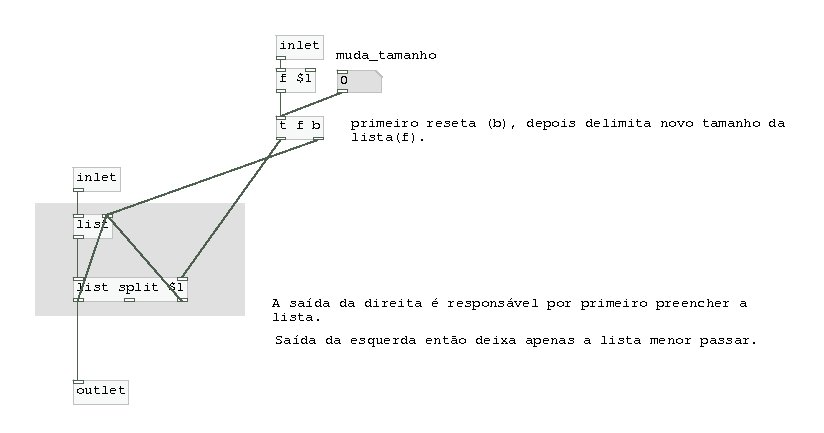
\includegraphics[scale=.5]{sinc-calc-ritmo2}
\caption{lista de durações}
\label{[sinc-calc-ritmo2]}
\end{figure}

\begin{figure}
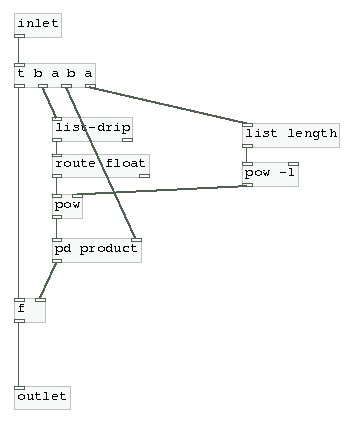
\includegraphics[scale=.5]{sinc-calc-ritmo3}
\caption{média geométrica}
\label{[sinc-calc-ritmo3]}
\end{figure}

\begin{figure}
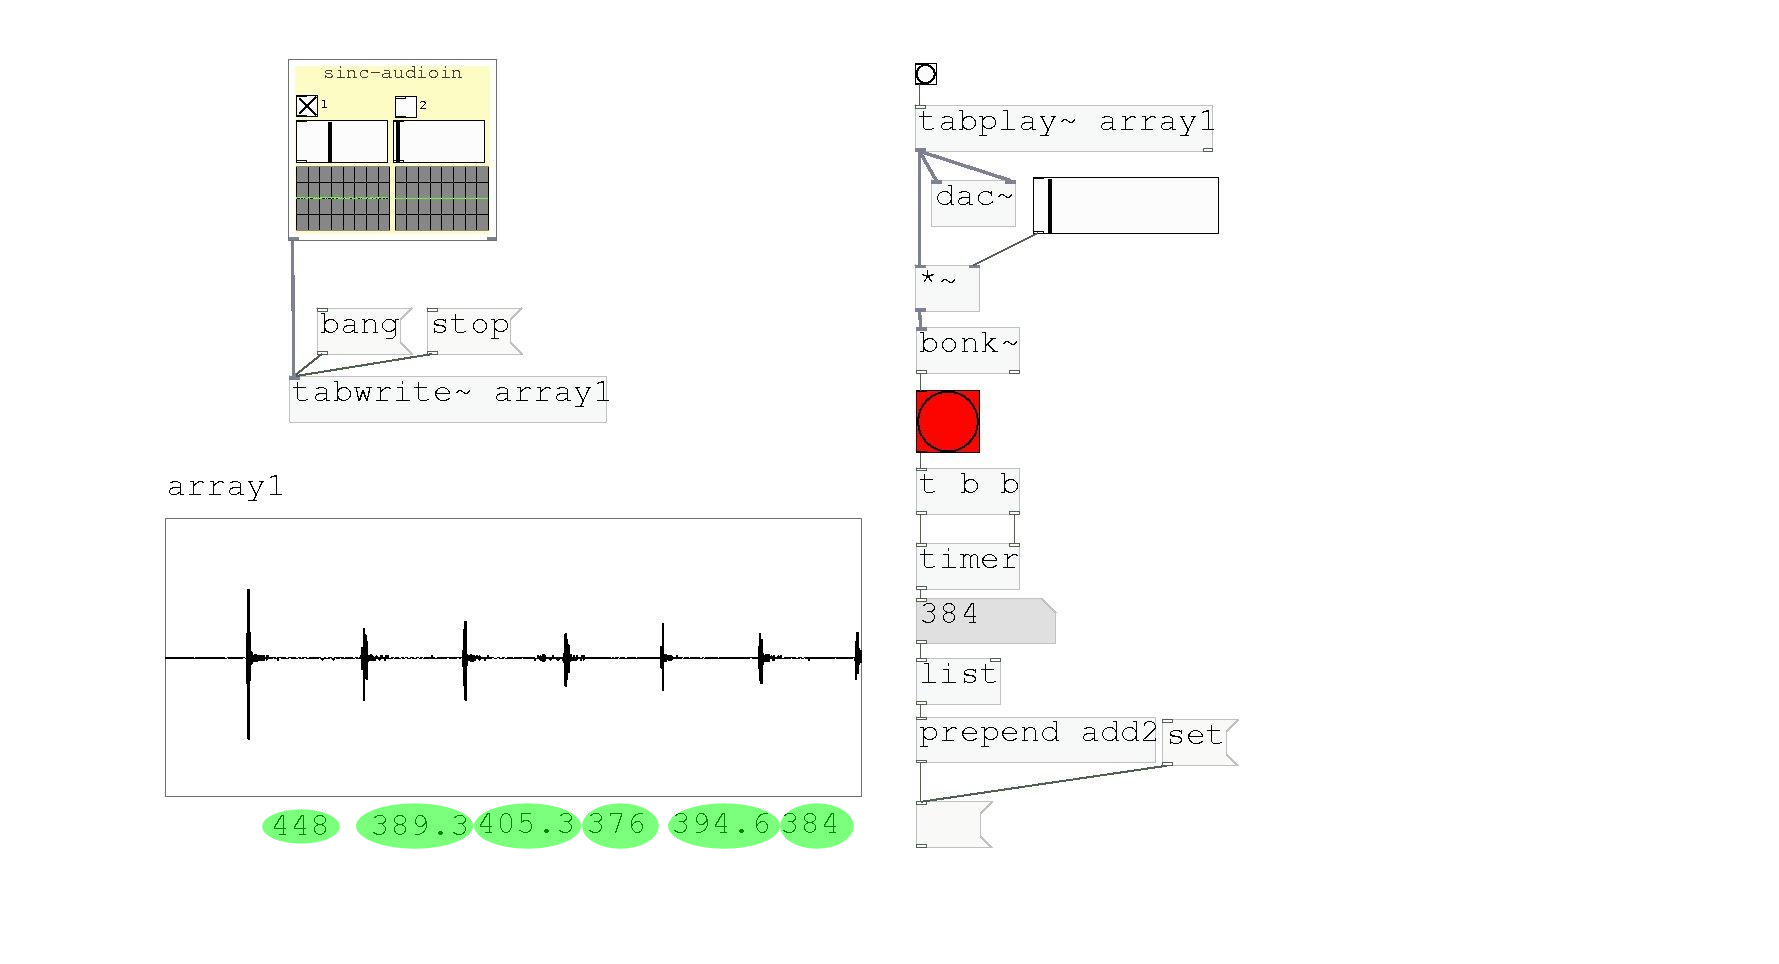
\includegraphics[scale=.5]{ex-ritmo1}
\caption{ritmo estável}
\label{ex-ritmo1}
\end{figure}

\begin{figure}
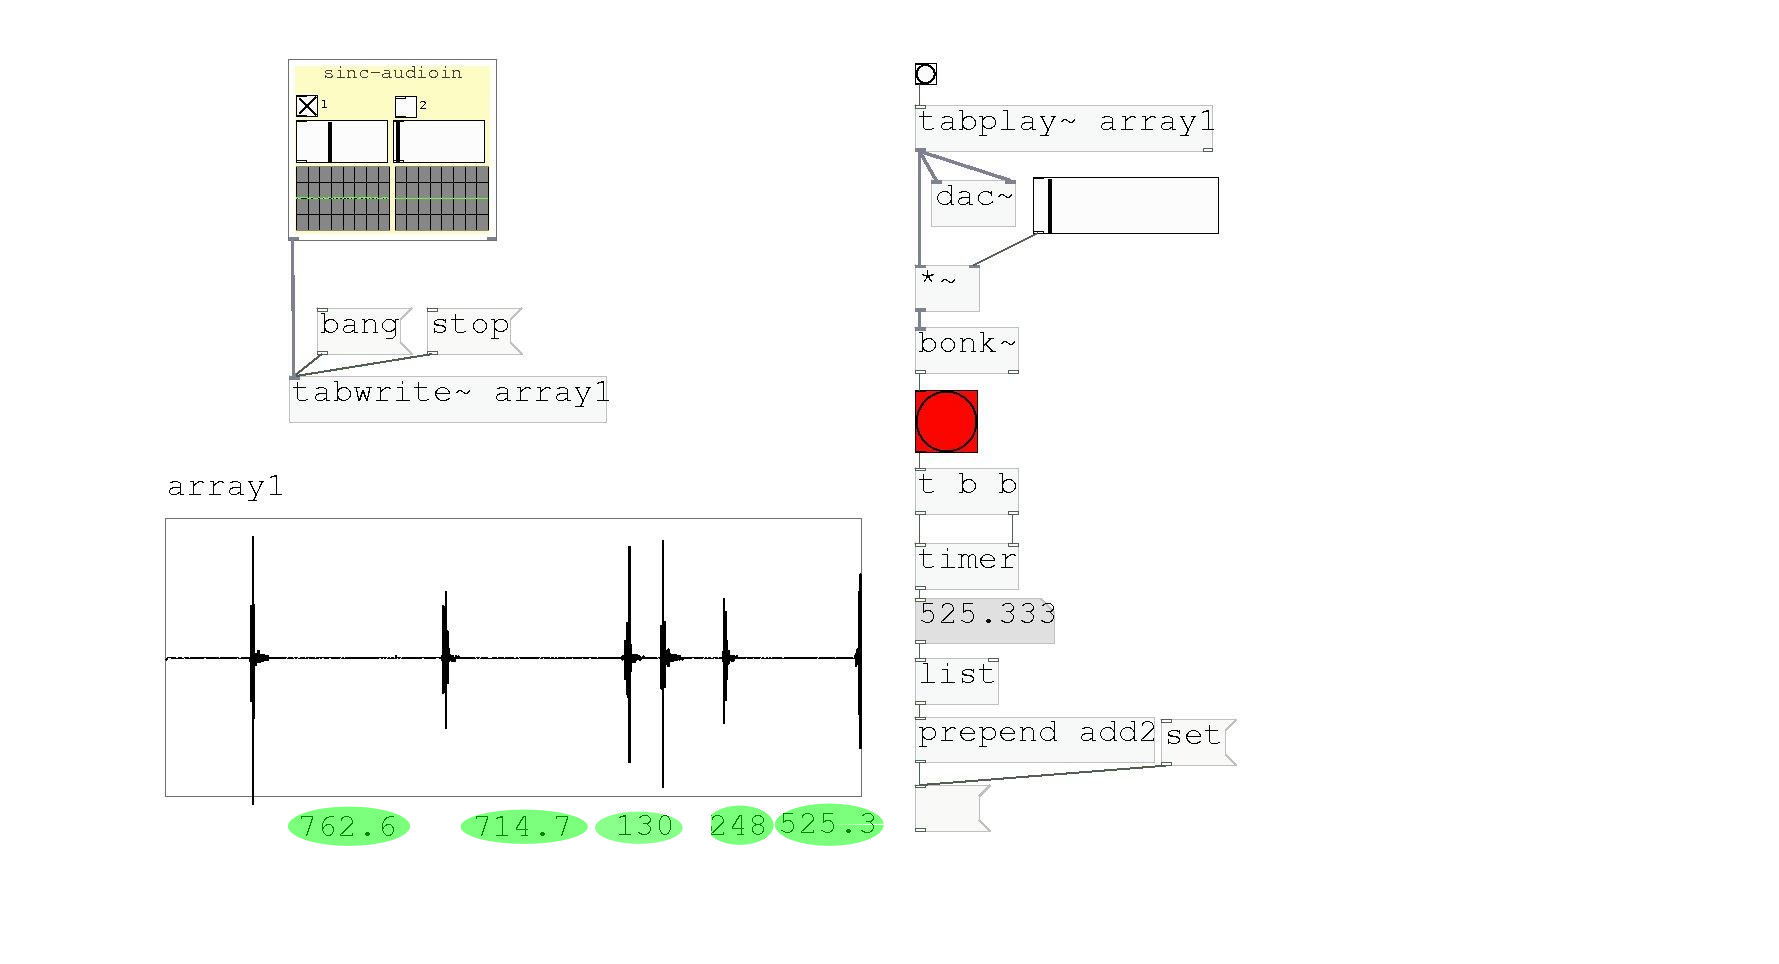
\includegraphics[scale=.5]{ex-ritmo2}
\caption{ritmo instável}
\label{ex-ritmo2}
\end{figure}

\begin{figure}
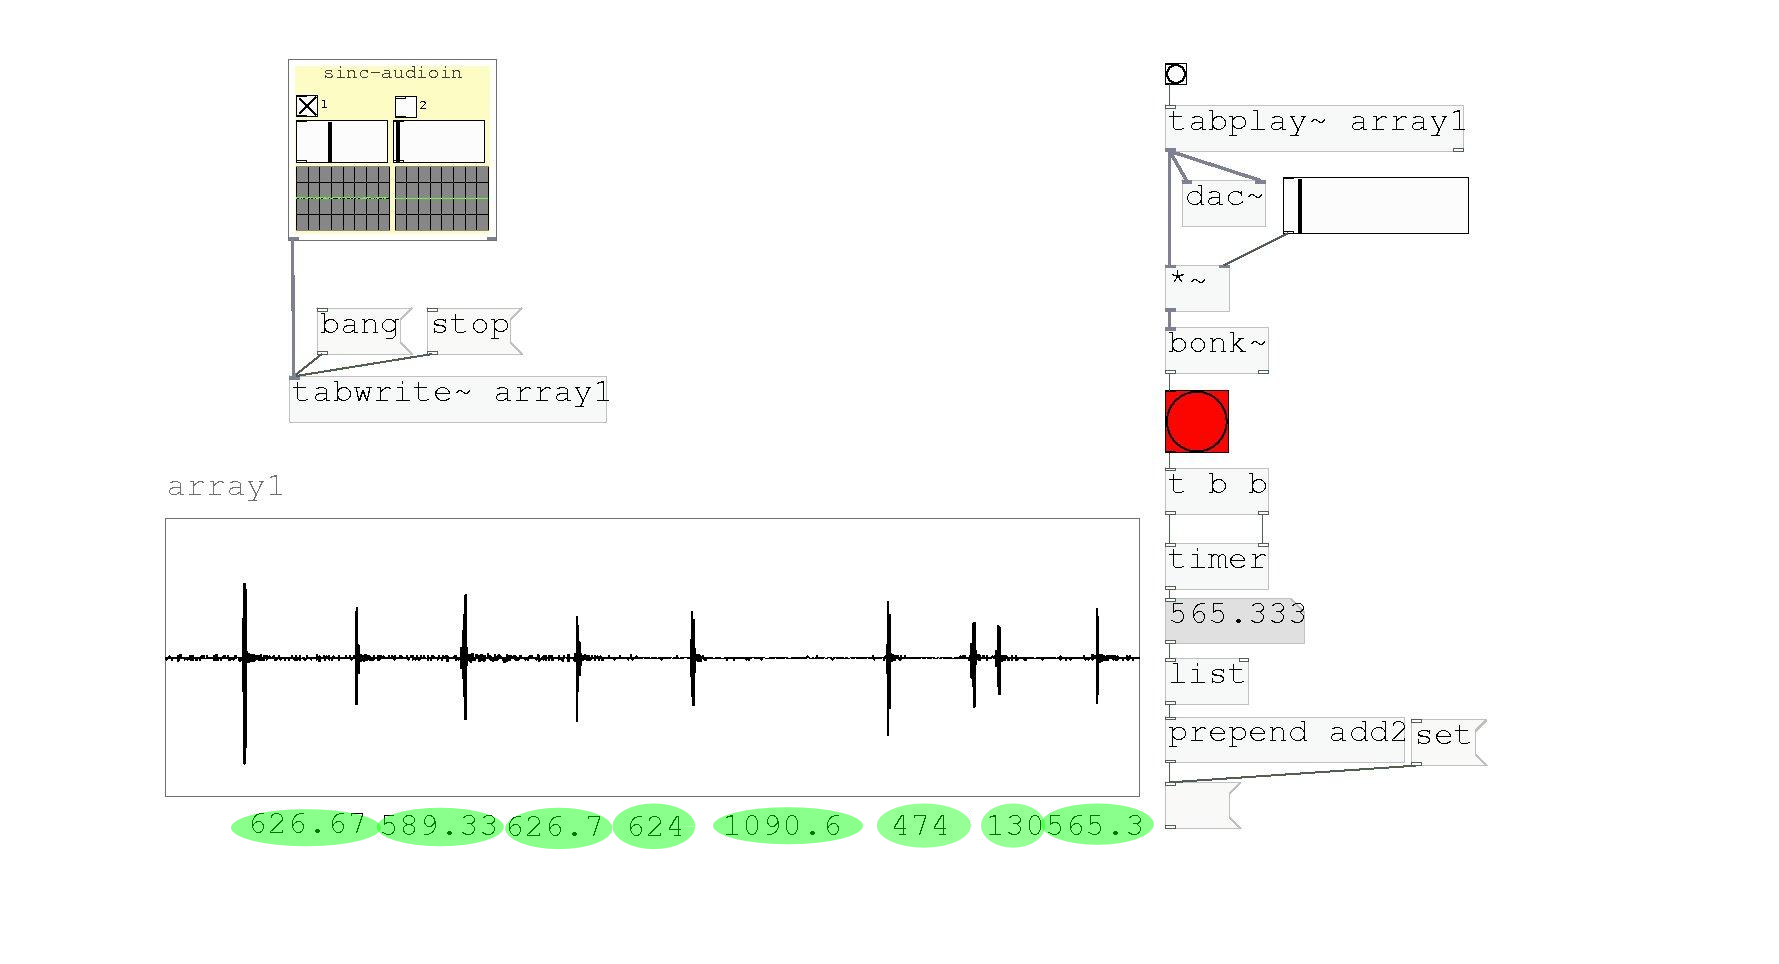
\includegraphics[scale=.4]{ex-ritmo3}
\caption{ritmo estável e instável}
\label{ex-ritmo3}
\end{figure}


A técnica básica de análise rítmica em Pd, se dá através do uso do objeto [timer].
O objeto [timer] mede a distância em milisegundos entre "bangs' que chegam pela entrada
da esquerda em relação ao que chega pela entrada da direita.%% aqui mostrar o básico do timer embasado pelo Rowe


Um músico humano sempre realiza micro-variações de tempo e andamento.
Na figura \ref{ex-ritmo1} vemos uma incidência de ataques mantendo uma relação de estabilidade
de durações. Enquanto que na figura \ref{ex-ritmo2} vemos uma relação mais instável
entre as durações. Já na figura \ref{ex-ritmo3} vemos um padrão que se mantém estável e 
muda para um comportamento de instabilidade de durações. Um dos desafios da pesquisa
foi estabelecer uma forma do programa conseguir classificar a estabilidade de cada nova duração em relação
as anteriores.

No patch da figura \ref{[sinc-calc-ritmo]} é apresentado um método de classificação de estabilidade
de durações entre notas. Primeiro são calculadas as distâncias entre cada ataque
sonoro, depois filtrado em [pd filter-range] e colocado em uma tabela dinâmica em
[pd last-x]. O tamanho da tabela sempre pode ser redimensionado em tempo-real através
da variável \textit{0-buffer-size} então é calculado ao mesmo tempo a média geométrica
e a média aritmética e os resultados são executados na expressão definida por uma
divisão da média geométrica pela média aritmética. %% isso poderia ser definido em notação matemática :)


A divisão da média geométrica pela média aritmética pode ser definida pela expressão

\begin{equation}
\frac{n\sqrt[n]{a1.a2....an}}{a1+a2+...an} 
\end{equation}  

Essa expressão é calculada a cada nota que chega, onde n é o tamanho do buffer.
O resultado desse cálculo devolve um valor numa escala de 0 a 1.
Esse valor representa o índice de instabilidade rítmica da última duração entre 2 notas,
comparado com as últimas "n" durações.
Nesse resultado dessa divisão é aplicado um filtro com [moses] onde se pode calibrar
a sensibilidade do valor do índice final.


\subsubsection{Objeto [sinc-densidade]}

%densidade-ritmica.pd em /abs


Densidade rítmica é o índice que mede a quantidade de eventos sonoros
dentro de espaços de tempo. Serve como ferramenta de análise e pode funcionar
como um parâmetro estrutural em um sistema de aálise musical mais completo.


\begin{figure}
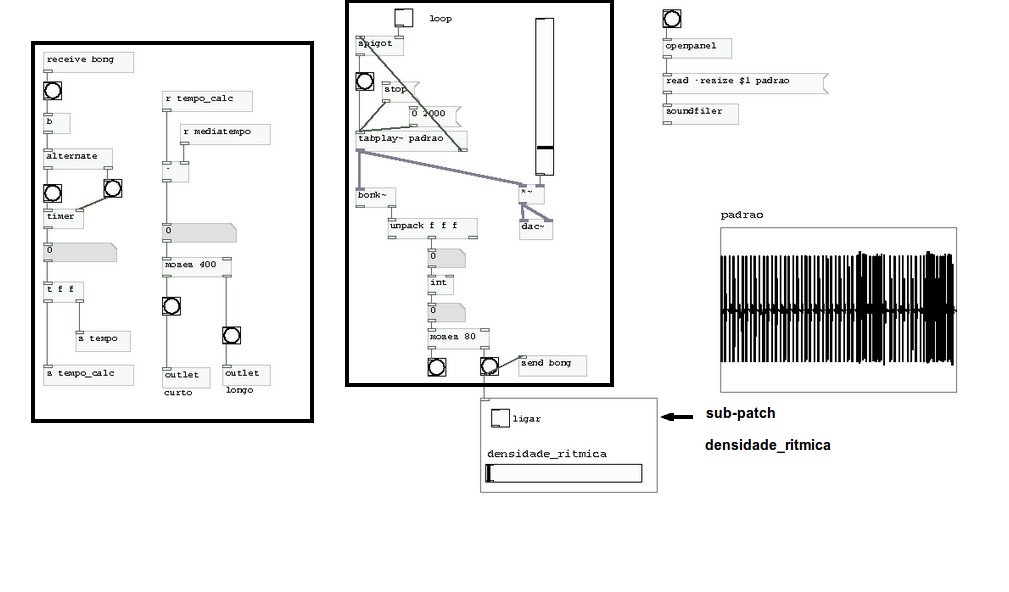
\includegraphics[scale=.5]{prot5b}
\caption{captação de ataques com [bonk\texttildelow] e categorização entre ``curtos'' e ``longos''}
\label{prot5b}
\end{figure}

Os primeiros passos na implementação de um mecanismo de análise de densidade podem ser vistos na figura \ref{prot5b},
onde na área central, aparecem um leitor de samples [tabplay\texttildelow] lendo um arquivo de
áudio e enviando o fluxo de áudio para o objeto [bonk\texttildelow]. A saída de [bonk\texttildelow] é filtrada
pelo objeto [moses] que pode ter um número de corte variável, sendo flexível a diferenças
de volume em diferentes momentos,lugares ou fontes sonoras .

Ainda na figura \ref{prot5b}, a seção da esquerda mostra uma maneira de classificar as durações
entre ataques de notas em longas ou curtas, possibilitando uma classificação básica,
que vai possibilitar a criação de padrões rítmicos de combinações entre longos e curtos.
Nesse caso também o limite entre longo e curto é dado por [moses] que pode ser redimensionado
em tempo-real. 

\begin{figure}
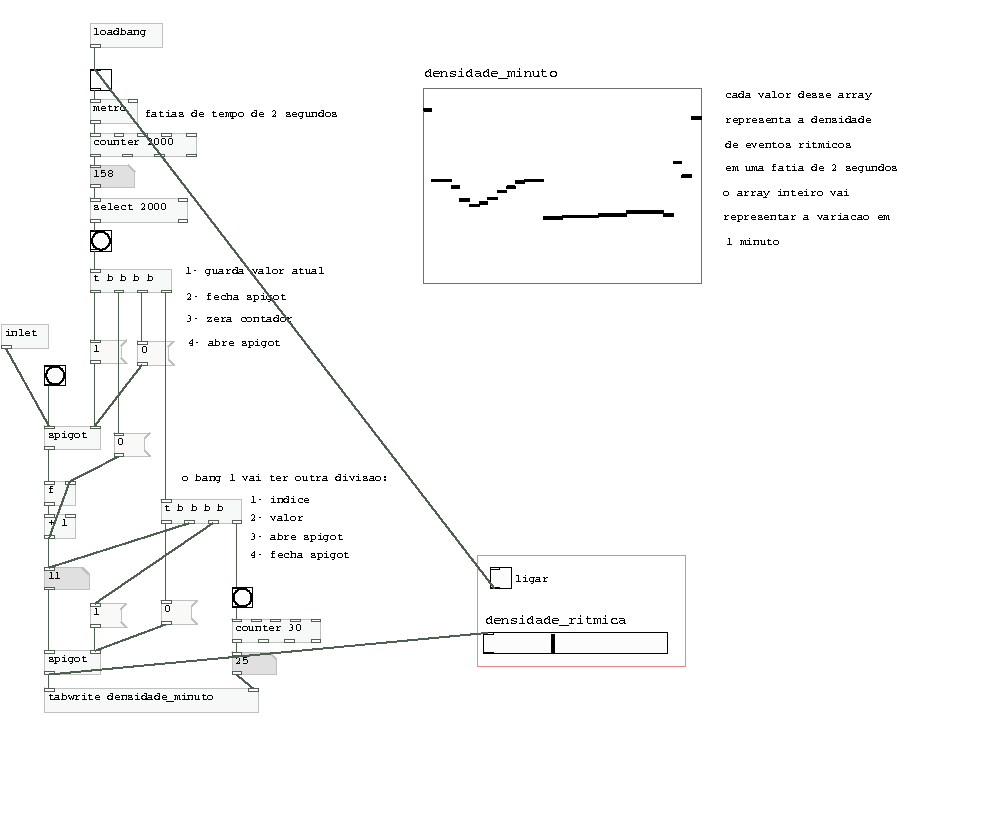
\includegraphics[scale=.75]{prot5c}
\caption{sub-patch [densidade ritmica]}
\label{prot5c}
\end{figure}


Na \ref{prot5c} vemos o conteúdo interno do sub-patch [densidade-ritmica], onde é realizadas
contagens de quantos ataques de eventos sonoros acontecem a cada 2 segundos de tempo.
Densidade rítmica é um bom índice global de controle dos eventos sonoros por um instrumentista.
A maneira de uso desse índice se transforma de um controle rítmico prático para um
músico treinado.





\subsection{Análise de timbre}

\subsubsection{FFT}

FFT é a sigla para Fast Fourier Transformation, e é a principal técnica para realizar uma análise no domínio 
da frequência. No Pd encontramos o objeto [rfft\texttildelow] que permite o 
acesso aos dados completos da análise do espectro sonoro.
Nessa seção será apresentada uma introdução sucinta a 
análise FFT no Pd e a manipulação dos dados resultantes dessa análise.

Uma explicação mais aprofundada da FFT no Pd é visto no apêndice \label{fftpd}.

* resumo rápido de FFT crua , acessando, visualizando e salvando e recuperando

\subsubsection{[bonk\texttildelow]}

%% colocar biblio; Miller (Real-time audio analysis tools for Pd and MSP) - 98

O objeto [bonk\texttildelow] possui um sistema interno de classificação
e comparação de amostras de áudio. Essa propriedade possibilita, por exemplo, 
uma situação de acompanhamento interativo para uma instrumentação de 
percussão múltipla.

Segundo Puckette:

\begin{quotation}
It is also possible to ask bonk to test any new at-
tack against a menu of pre-recorded attacks in order
to guess which of several possible instruments was
responsible for the new attack. To do this, first we
store spectral templates for each of the instruments.
Thereafter, any new attack is compared with the
stored ones and the closest match is reported. The
underlying assumption, that there is actually some
repeatability in the spectral envelopes of attacks of
percussive instruments certainly doesn't hold true in
the real world, but it is interesting to learn which
sorts of instruments bonk can identify in this way
and which it can't.
\end{quotation}

O objeto [bonk\texttildelow] pode funcionar detectando
ataques em tempo-real retornando um bang para cada ataque 
na saída esquerda. Ou então pode alternar entre dois estágios:
"learn" e "forget" que são enviados como mensagem na entrada de 
[bonk\texttildelow]. Outras mensagens posicionam outros
parâmetros como por exemplo "minvel", para mínima amplitude de offset
para retornar uma detecção de ataque.
Se for enviada uma mensagem com "learn 10",
o objeto irá aguardar dez notas consecutivas do mesmo instrumento.
O resultado da comparação interna é retornado pela saída da direita.



\subsubsection{timbreID}

\begin{figure}
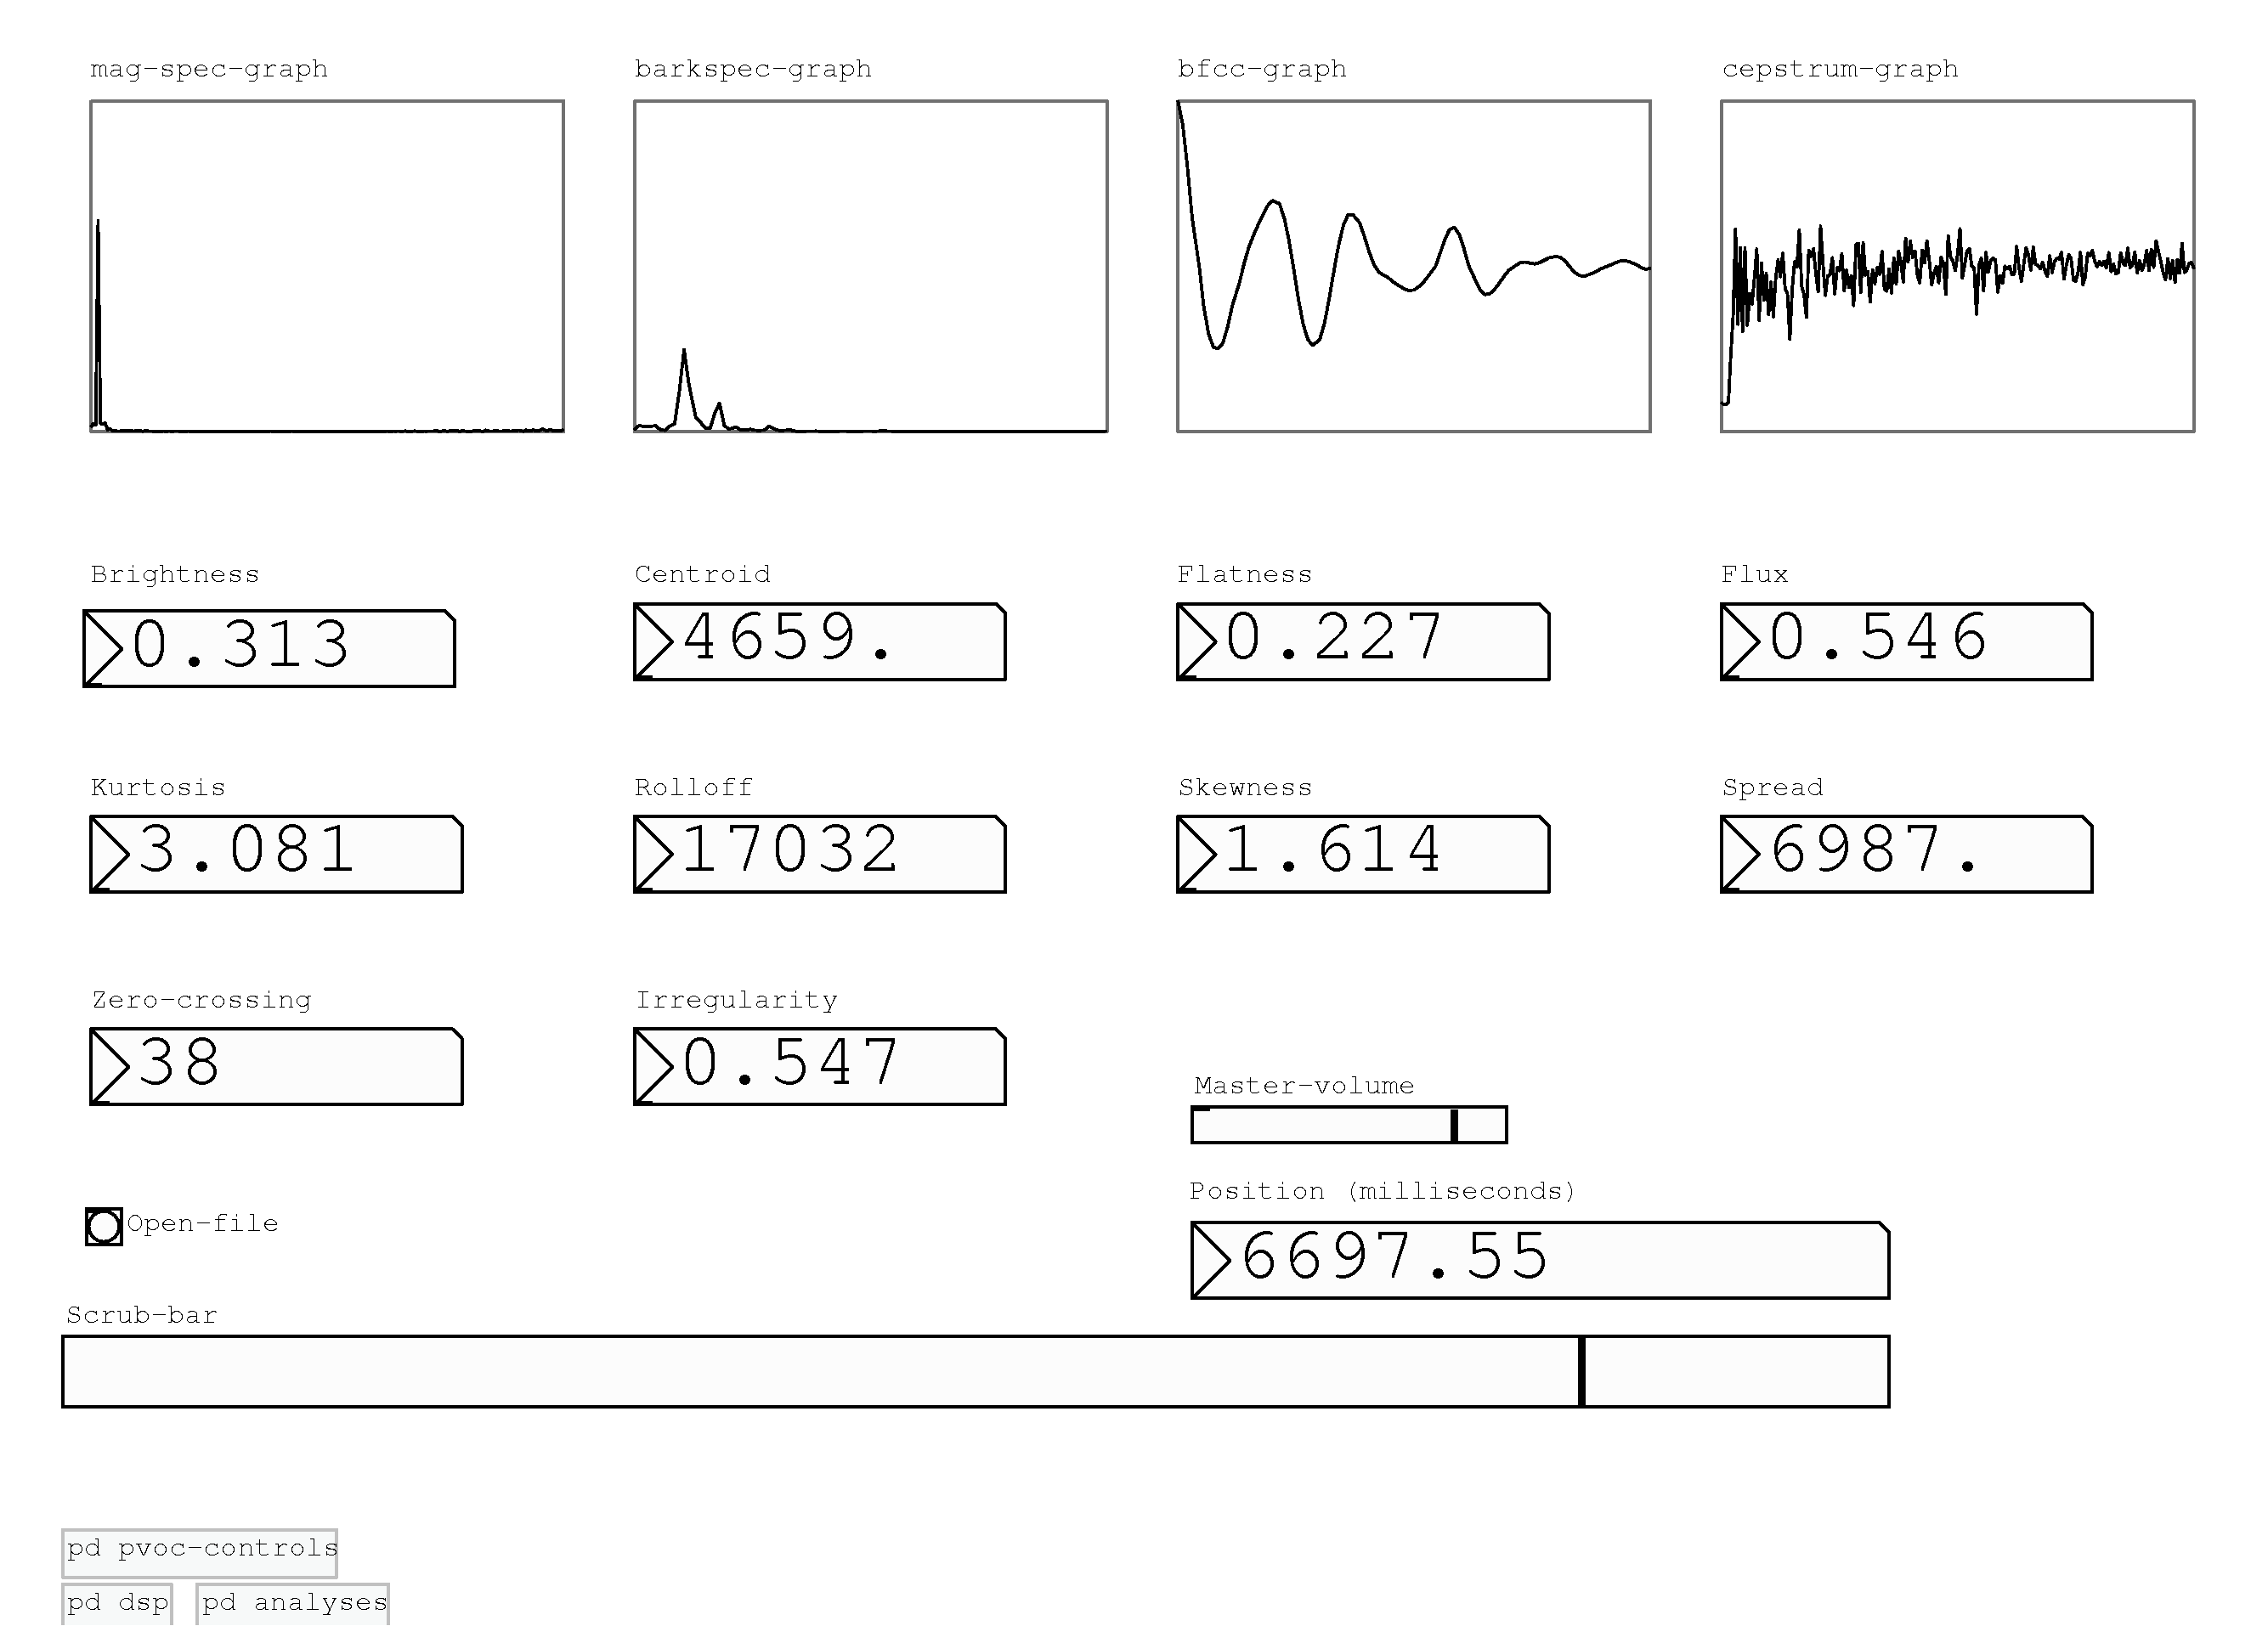
\includegraphics[scale=.6]{audio-features}
\caption{audio-features}
\label{audio-features}
\end{figure}

\begin{figure}
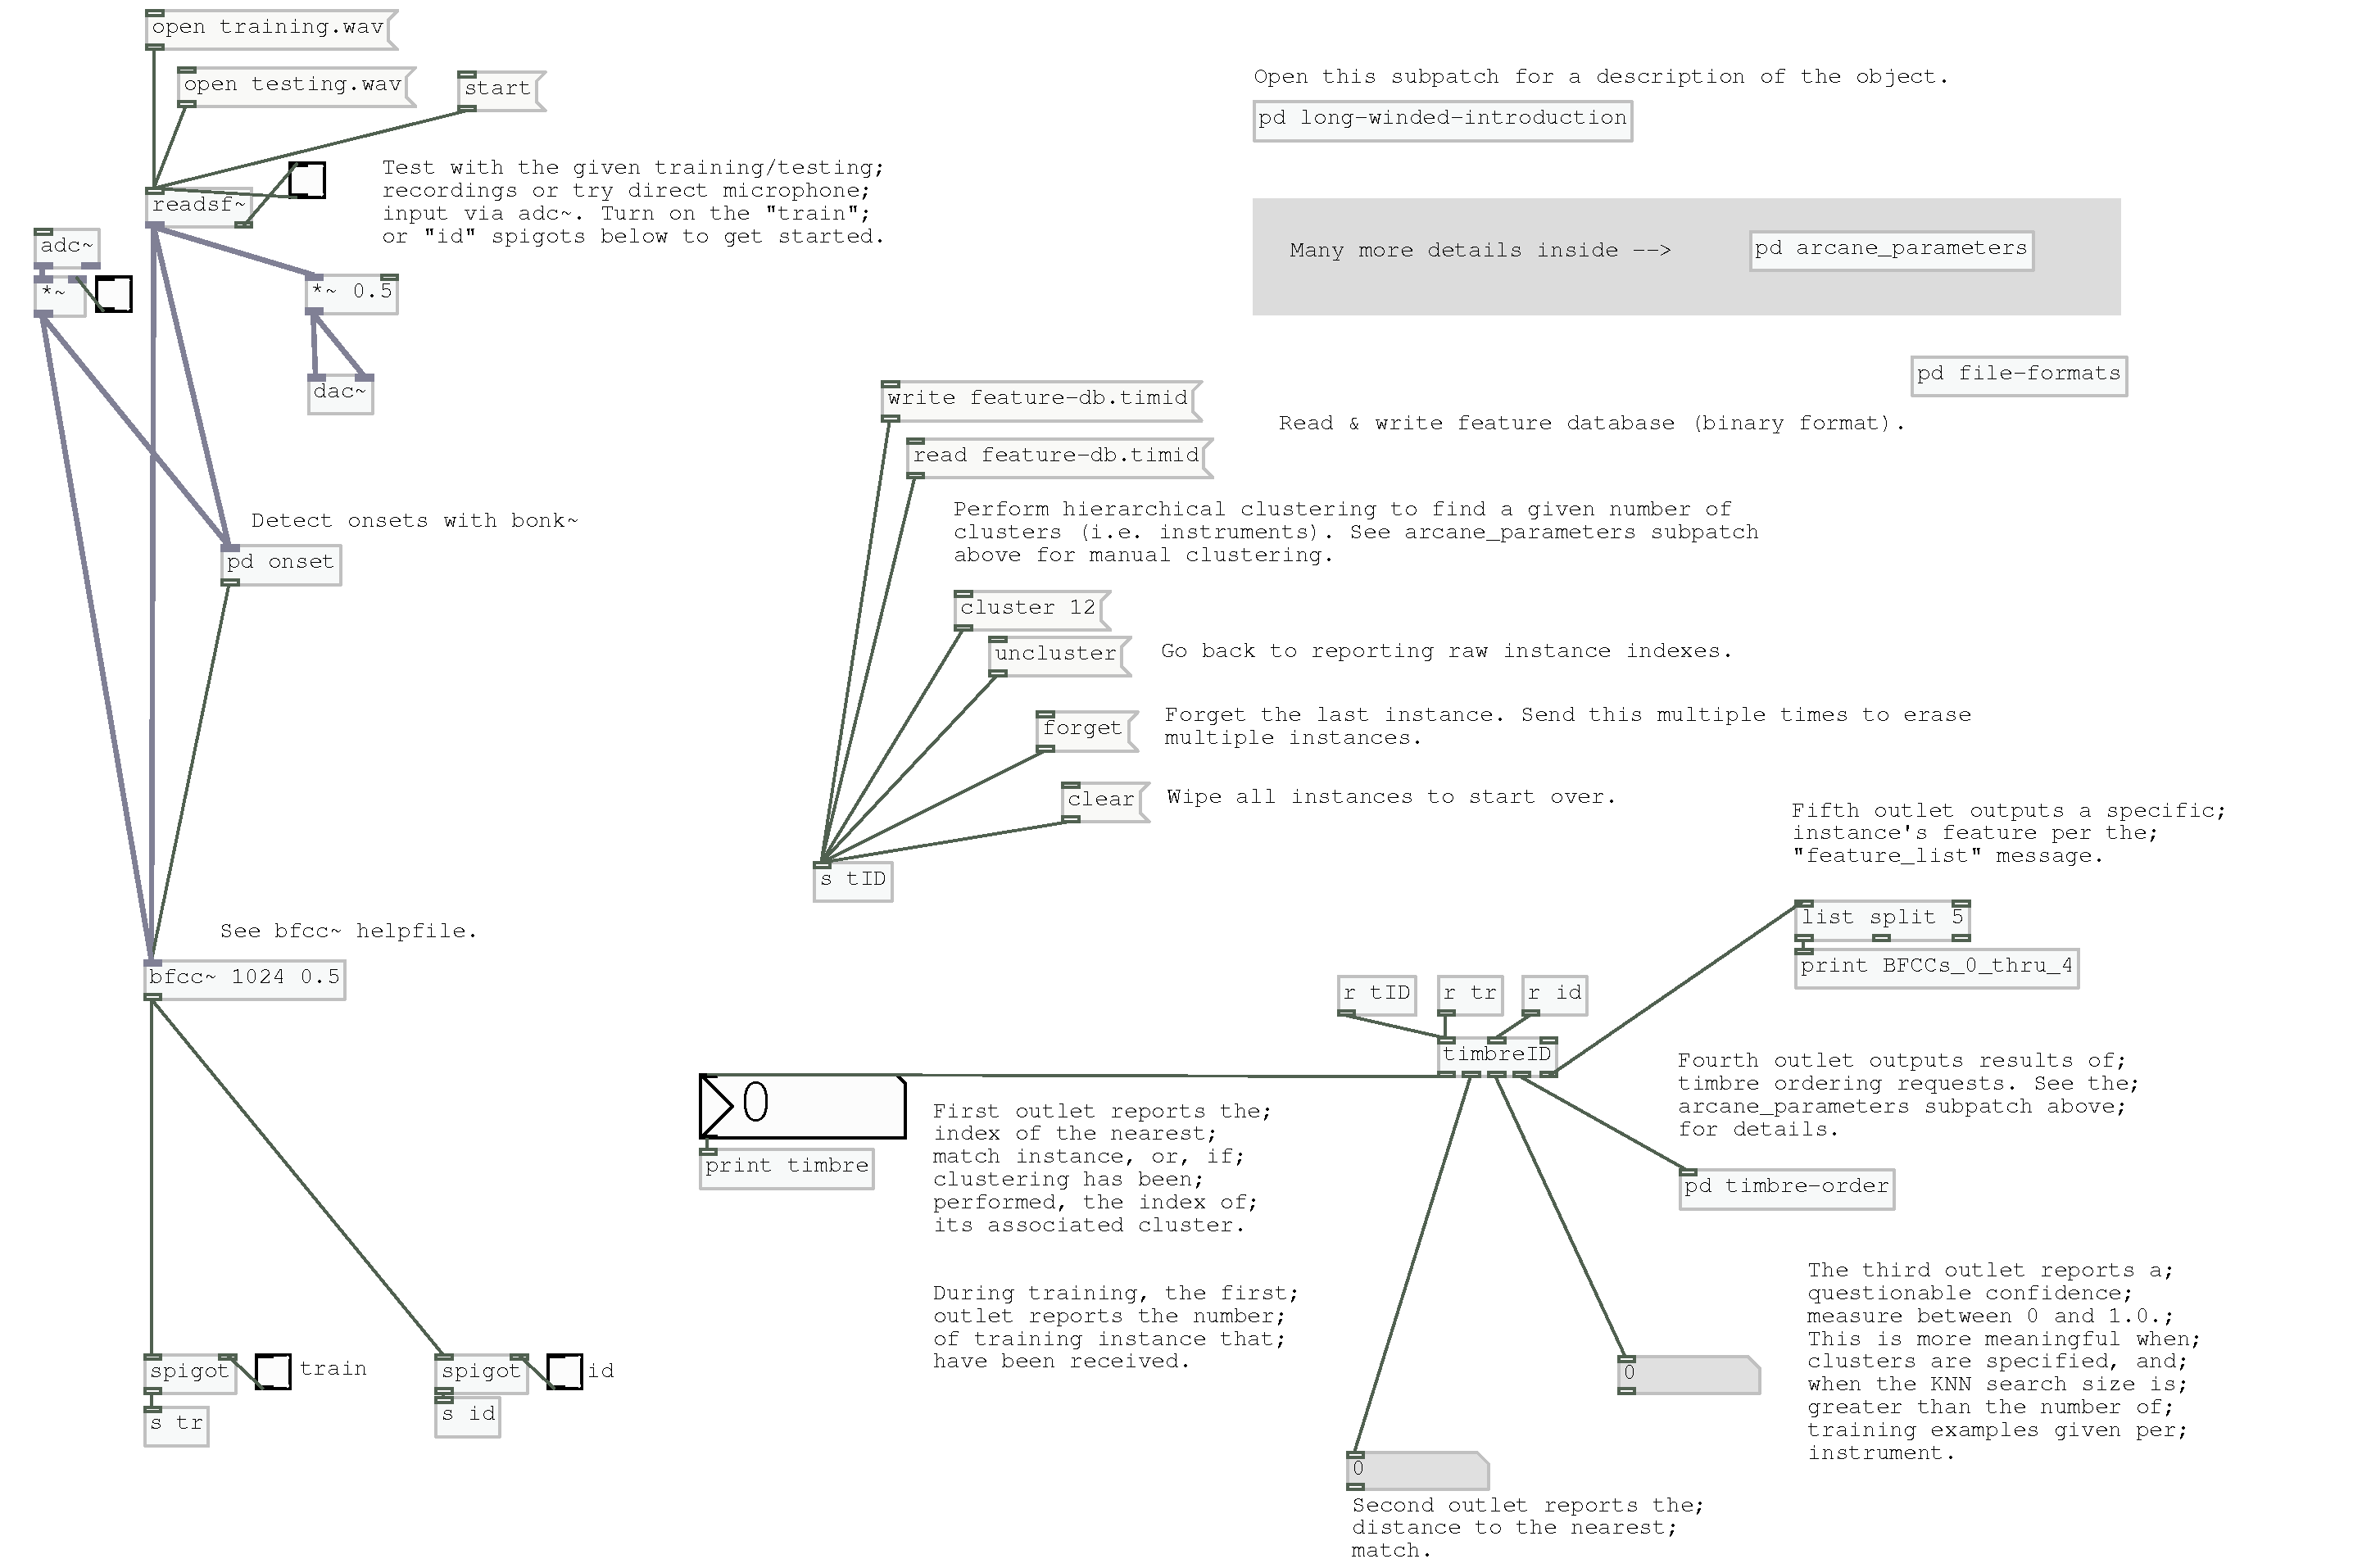
\includegraphics[scale=.6]{timbreid}
\caption{timbreID}
\label{timbreid}
\end{figure}

\begin{figure}
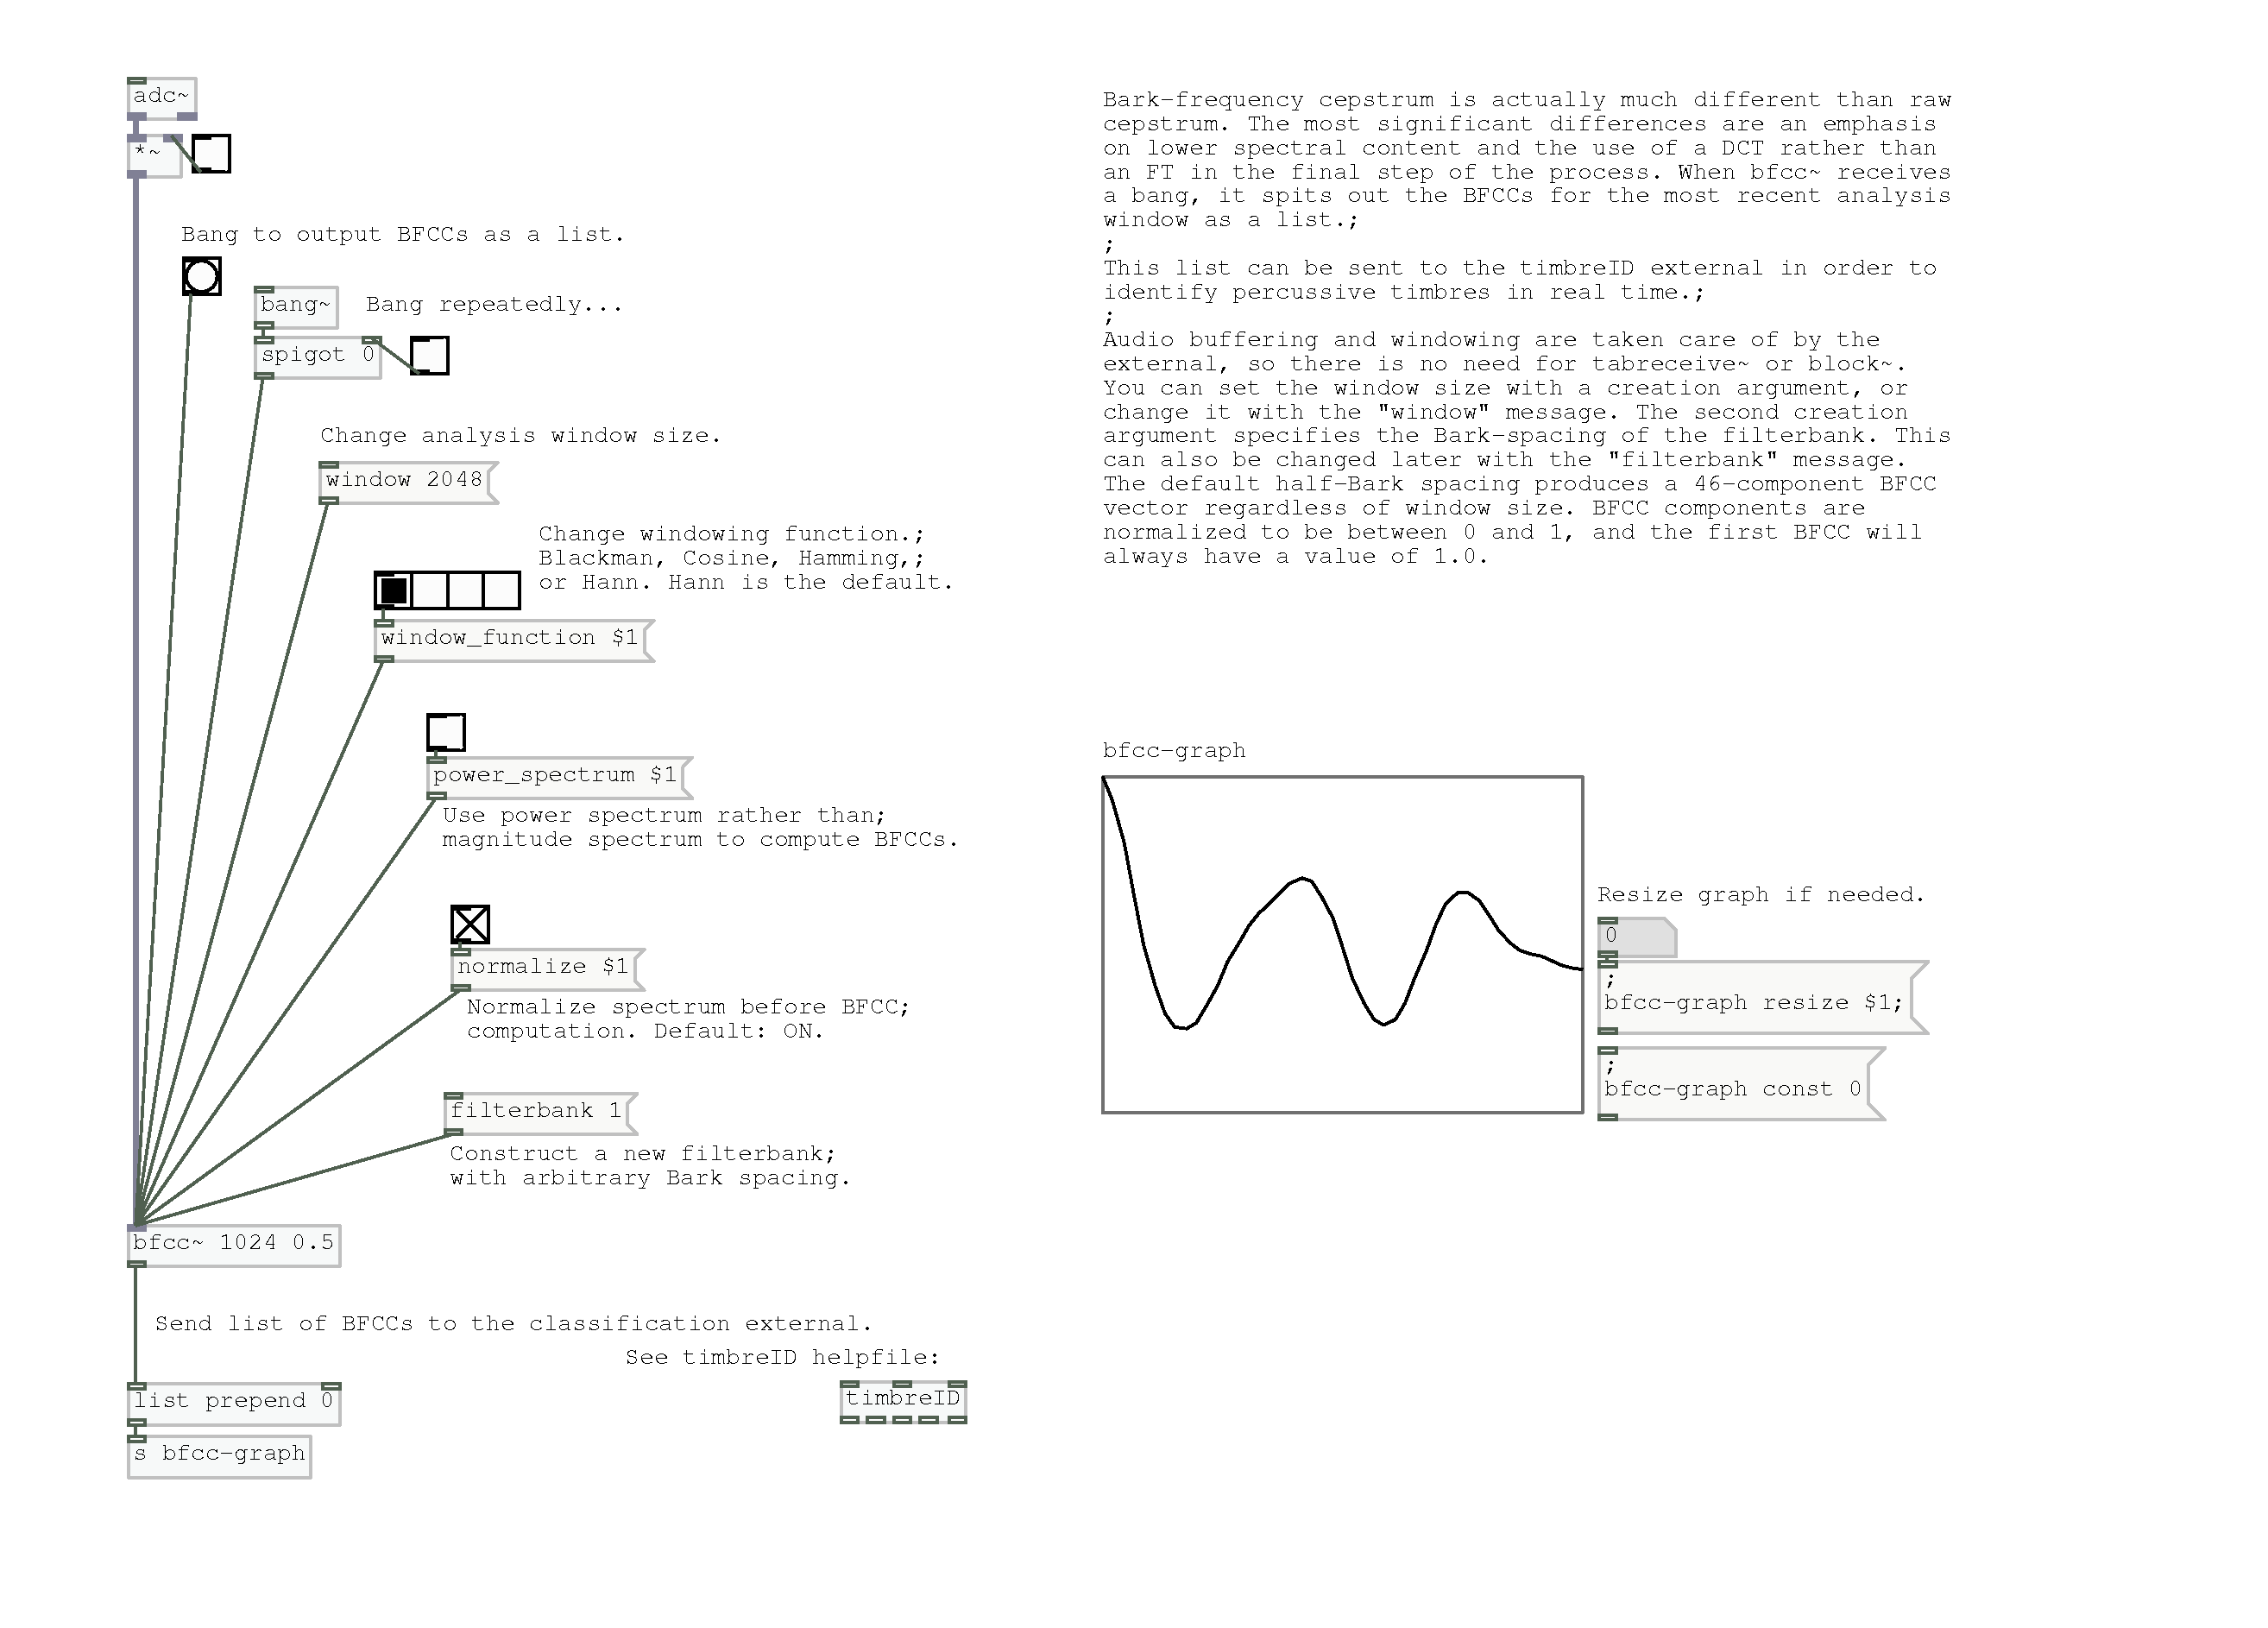
\includegraphics[scale=.6]{bfcc}
\caption{bfcc}
\label{bfcc}
\end{figure}

\begin{figure}
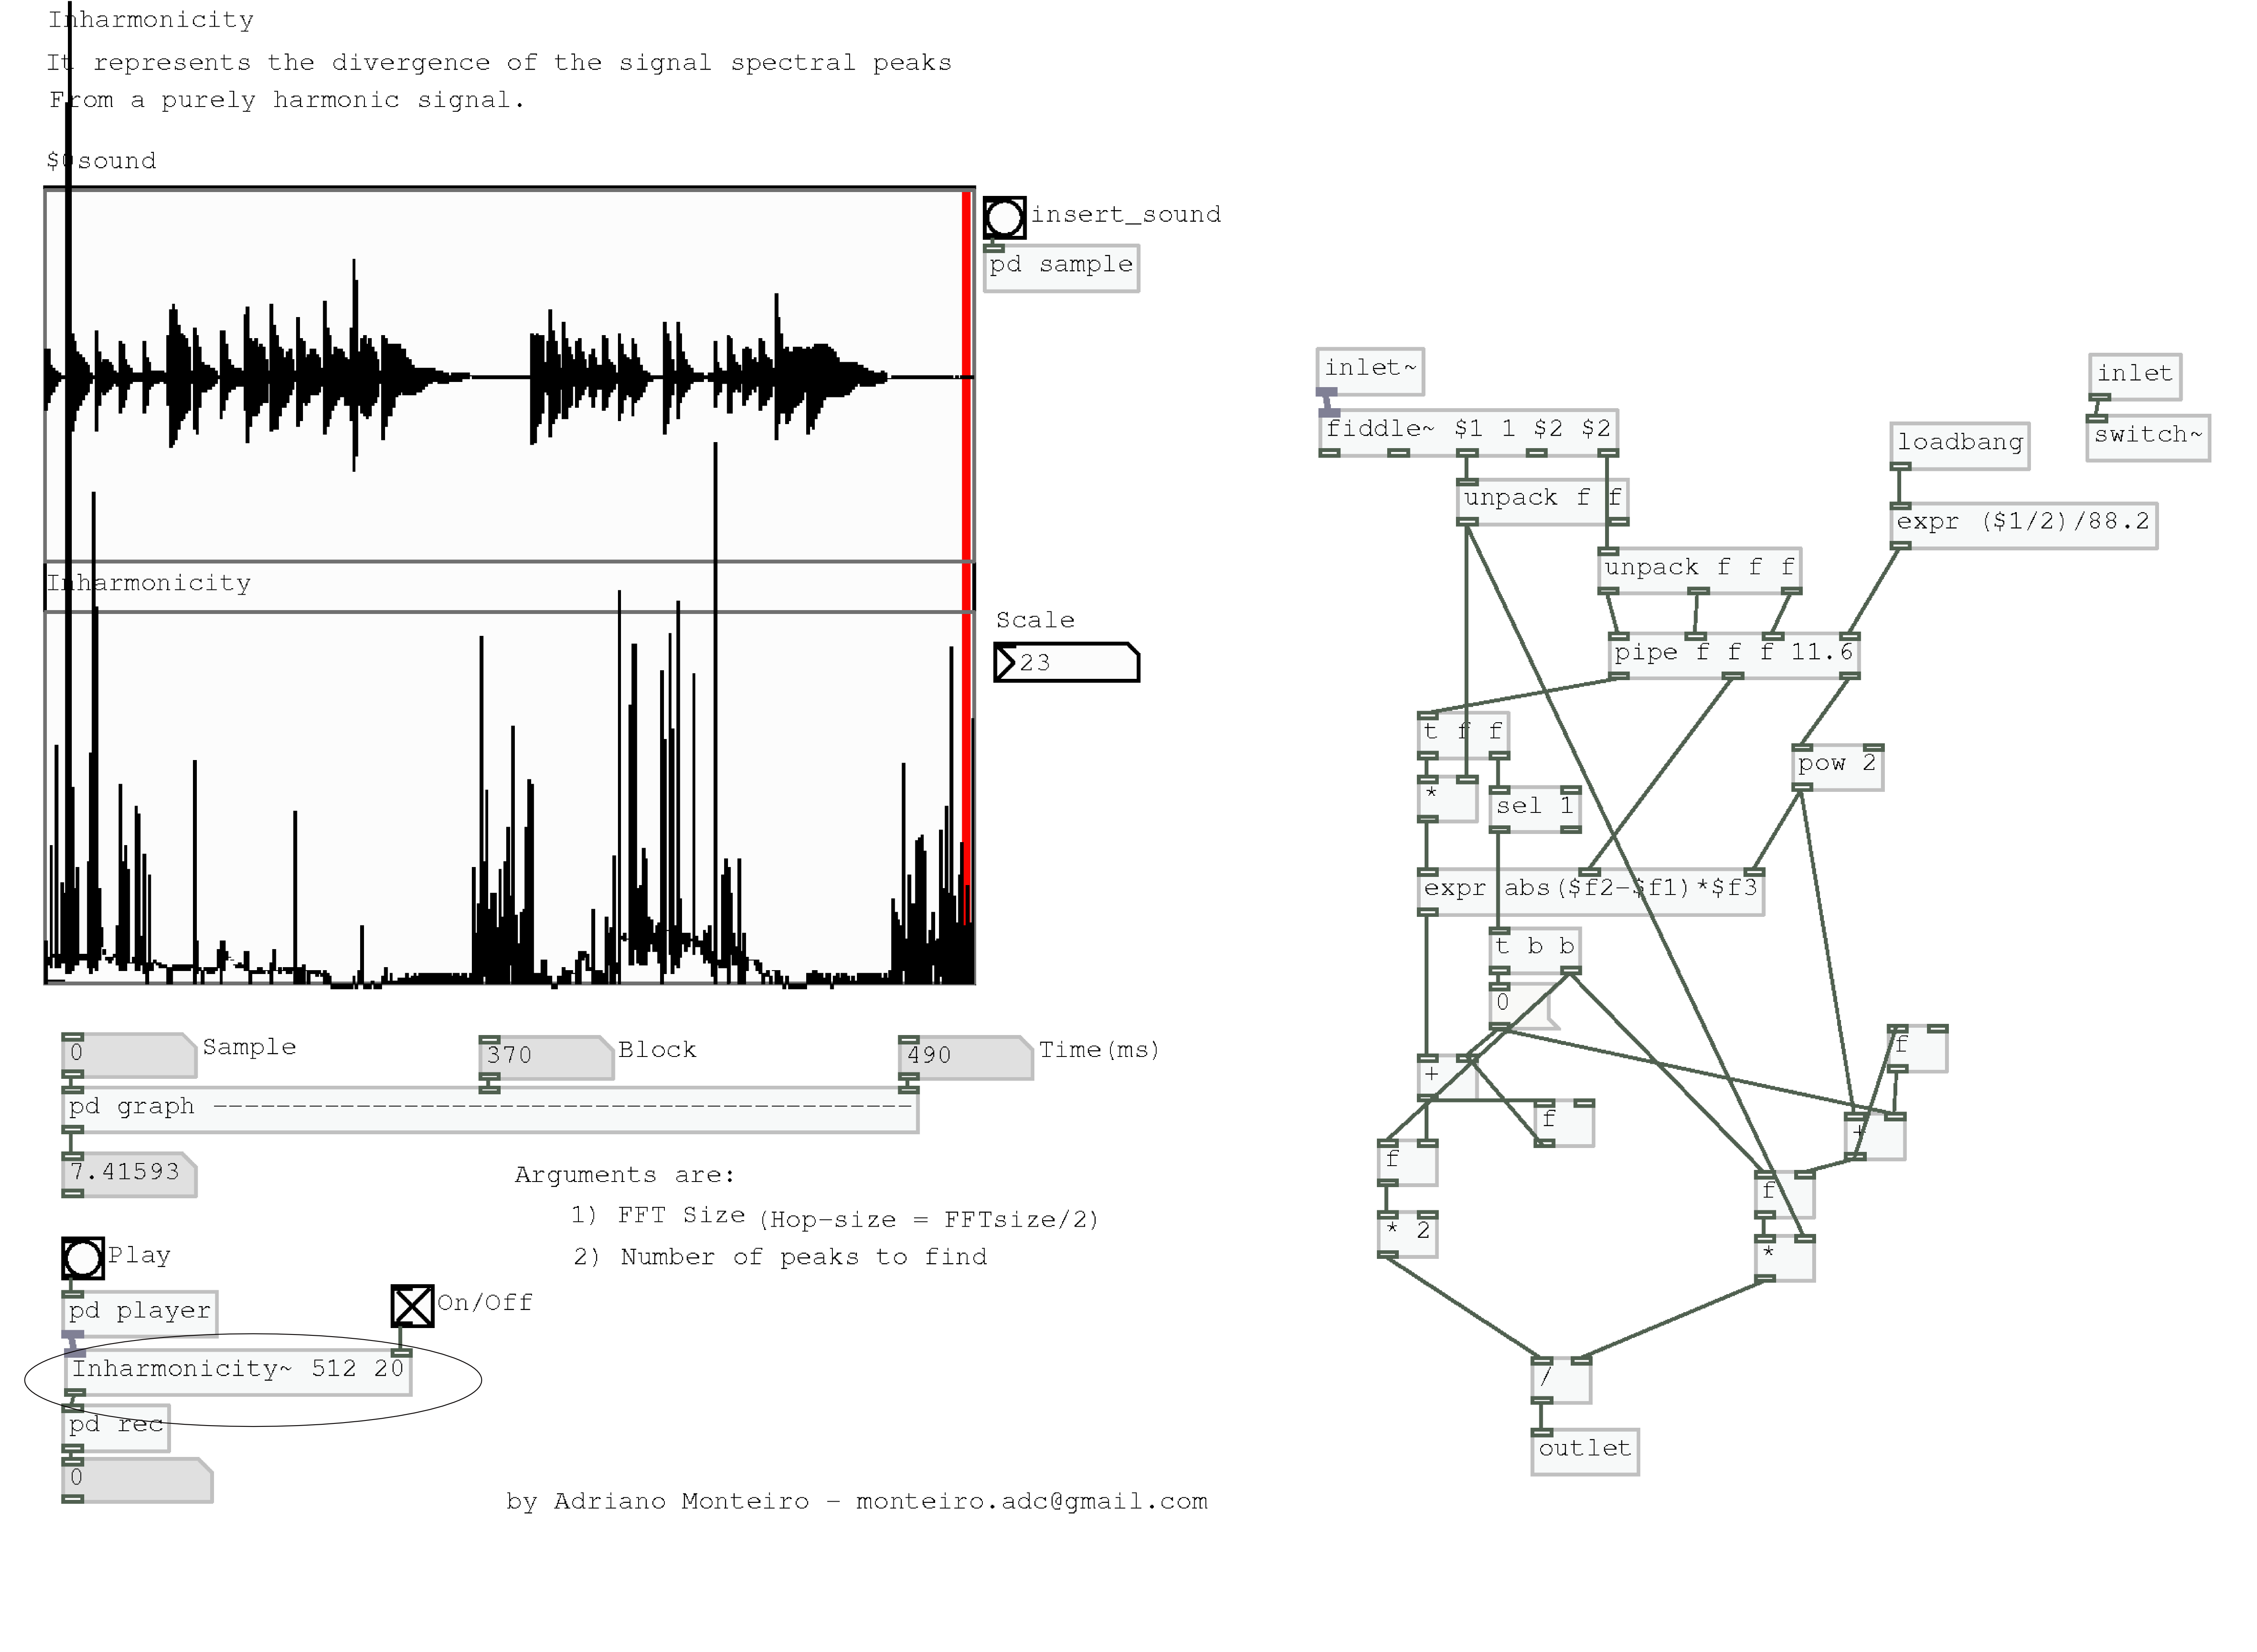
\includegraphics[scale=.7]{pdescriptor}
\caption{PDescriptors - [Inharmonicity\texttildelow]}
\label{pdescriptor}
\end{figure} 


Quando se acessa aos dados puros da de um fluxo de áudio precisamos de 
métodos específicos para filtrar esses dados. Uma densa bibliografia
tem sido desenvolvida sobre algoritmos de busca e filtragem de dados de
análise FFT. Cada algoritmo é especializado em algum aspecto, seja de
estimativa de frequência fundamental, ou de comportamento espectral da fonte sonora,
como por exemplo, estimativa se determinado trecho é uma nota com articulação diferente
ou um ruído indesejado.
Pode-se dizer que a filtragem dos dados de análise espectral é um importante
núcleo dentro da pesquisa em música interativa e computação musical. Nessa seção
serão comentadas algumas ferramentas que demonstram o estado da arte da análise de 
áudio em tempo real, que permitem um maior refinamento na detecção de parâmetros
sonoros em projetos de música interativa.

Nese sentido, além dos dados puros da FFT feita com o objeto [rfft\texttildelow],
destacamos duas bibliotecas externas de Pd que compreendem diversos algoritmos
diferentes de análise. A primeira biblioteca é a 
timbreID desenvolvida por William Brent e compreende uma série de objetos
implementados em C e possui uma boa eficácia em processamento. A timbreID possui 
quatorze objetos de análise espectral cada um em versão estática e tempo-real, com a diferença
de que a versão em tempo-real processa áudio em vez de valor de amostra. Além
de um objeto classificador [timbreID]. Na figura \ref{timbreid} temos
uma visão geral de um dos algoritmos de análise do objeto  [bfcc\texttildelow], baseado na 
análise Cepstral enviando dados para o classificador [timbreID]. Na figura \ref{bfcc} podemos
ver em detalhe o funcionamento de [bfcc\texttildelow].

Segundo Brent:

\begin{quotation}
 Bfcc~ is the most developed cepstral external, using the more thoroughly researched Bark scale rather than mels for 
the spectrum weighting. Performance is only slightly better than mfcc~. The most noteworthy thing about these cepstral 
externs is the flexibility they provide with respect to filterbank construction. The choice of a specific Bark- or 
mel-spacing can have a real impact on how relevant the features are in classifying one sound set vs. another.
\end{quotation}


Uma das vantagens da timbreID é a flexibilidade de parametrização. A biblioteca é dividida
entre objetos externos para implementação de cada algoritmo e um objeto responsável pela
classificação dos resultados dos algoritmos. O objeto de classificação ([timbreID]) aceita
listas de características timbrísticas e tenta encontrar a melhor correspondência entre cada 
característica do áudio de entrada e instâncias estocadas dos dados treinados.
Listas de características mandadas para a entrada da esquerda são processadas pela função
"train" (em formato de mensagem). Isso fornece exemplos das características que sobre as quais
futuras comparações serão baseadas. Uma vez que uma base de dados de treinamento é criada, ela
pode ser salva em um arquivo .timid com o método "write", e mais tarde recuperado com o método
"read". Outros formatos de saída são .txt, .mat (para uso com os programas MATLAB ou Octave)
e ARFF (para uso com o ambiente WEKA).

A segunda entrada do objeto [timbreID] recebe listas de características que são comparadas com
aquelas no banco de dados do treinamento e uma correspondência é identificada. As instâncias de 
correspondência são distinguidas pelo índice, por isso, se a correspondência mais próxima for o 
índice 7, o número 7 vai aparecer na primeira saída da esquerda.

Na figura \ref{audio-features} vemos um painel geral com os resultados simultâneos dos quatorze
algoritmos de análise espectral diferentes. Notamos que os quatro objetos superiores retornam resultados em 
listas que são plotadas em arrays, enquanto os demais objetos retornam índices puros.

Outra  biblioteca relevante é a PDescriptors desenvolvida 
por Adriano Monteiro e se tratam
de abstrações de Pd que usam apenas objetos "vanilla" e por isso possui um
grande poder de compatibilidade com diversos projetos. As abstrações
são divididas em características perceptuais, espectrais, harmônicas e temporais, além
de alguma ferramentas de transcrição. Podemos ver a interface do objeto [Inharmonicity\texttildelow]
na figura \ref{pdescriptor}, onde o resultado da análise é plotado no gráfico abaixo da forma de 
onda da fonte, o que facilita a comparação visual, resultando numa boa interface para trabalho de análise de áudio.



%texto original:
% Listas de características enviadas para a terceira entrada também produz correspondências, mas esta entrada é projetada especificamente para
% síntese concatenativa . Outras mensagens que direta e restringir a pesquisa do banco de dados pode ser usado em combinação
% com esta saída. Veja o exemplo granular na [pacote exemplos timbreID] para uma explicação detalhada, e
% ouvir isso [exemplo de som] de uma voz reconstruída usando grãos a partir de um arquivo de som de instrumentos de corda friccionada.
% [Este exemplo de som] reconstrói a amostra mesma voz usando grãos a partir de um arquivo de som de ruidosos de baixa qualidade
% efeitos sonoros dos desenhos animados. Ambos os exemplos começar com apenas a voz, em seguida, desaparecer na reconstrução em tempo real granular
% da voz, então fade out a voz.
% 
% • Feature lists sent to the third inlet also produce matches, but this inlet is designed specifically for 
% concatenative synthesis. Other messages that direct and restrict the database search can be used in combination 
% with this outlet. See the granular example in the [timbreID examples package] for a detailed explanation, and 
% listen to this [sound example] of a voice reconstructed using grains from a sound file of bowed string instruments. 
% [This sound example] reconstructs the same voice sample using grains from a sound file of noisy low-quality 
% cartoon sound effects. Both examples start with just the voice, then fade in the real-time granular reconstruction 
% of the voice, then fade out the voice.
% 
% 
% 
% • Um algoritmo de clustering pode ser executado usando o "cluster" da mensagem, após o qual as instâncias serão agrupados em uma
% número desejado de clusters que representam instrumentos. Desta forma, não há necessidade de especificar exatamente quantos
% exemplos serão dados durante o treinamento. Depois de clustering, timbreID irá imprimir o índice cluster associado de
% a instância que melhor combinam com. Quando casos foram agrupados em clusters, de correspondência é realizada utilizando uma
% k-vizinhos mais próximos, estratégia, para o qual você pode especificar k. Se o cluster automática não funcionar, ou se você
% desejo de sons diferentes do grupo em conjunto, uma opção manual também está disponível.
% 
% • A tomada de quarto relatórios listas de ordenações com base em dados timbres de partida. Desta forma, você pode analisar um conjunto
% de sons e têm timbreID propor ordenações que tenham transições timbre suave. Veja o exemplo timbre ordem
% na [pacote exemplos timbreID] para uma explicação detalhada. Você também pode ouvir isso [exemplo de som] de um
% conjunto de sons reproduzidos em ordem aleatória seguido por uma ordem produzido por timbreID. Outros exemplos podem ser pedidos
% ouvido abaixo.
% 
% • pesos individuais podem ser atribuídos a característica componentes da lista. Por exemplo, se sua lista de recurso consiste em
% BFCCs e centróide, você pode peso este último a ser metade tão influente como o primeiro para calcular a distância.
% 
% • Uma vez que o tamanho da lista é arbitrária, uma forma eficaz para capturar a evolução temporal de um som é para concatenar
% os resultados da análise de múltiplas janelas sobrepostas. Esta estratégia de análise é usado no exemplo timbre ordem na
% [TimbreID pacote de exemplos], e os gráficos das análises podem ser vistas como elas ocorrem em tempo real.
% 
% 
% O recurso mais poderoso externs são baseadas na análise cepstral. cepstrum ~ saídas do cepstrum-prima de uma análise
% frame, e MFCC ~ é outra versão que distorce o resultado inicial FFT para a escala de freqüência mel. Claramente executa
% mais confiável. A técnica de MFCCs decorrentes é descrito em Rabiner \ & Fundamentos Juang de Reconhecimento de Voz.
% Em suma, todas as bandejas de FFT são executados através de um composto de sobreposição filterbank filtros triangular, ferver a
% espectro de até 20 ou mais números, que são então submetidos a uma transformada discreta de cosseno. Essa ponderação do
% eixo da freqüência pode ser mais de acordo com a forma como percebemos timbre.
% 
% bfcc ~ é o mais desenvolvido cepstral externo, utilizando a escala Bark mais profundamente pesquisados, em vez de Mels para
% a ponderação do espectro. Desempenho é apenas ligeiramente melhor do que MFCC ~. A coisa mais notável sobre essas cepstral
% externs é a flexibilidade que eles fornecem no que diz respeito à construção filterbank. A escolha de um determinado Bark ou
% mel espaçamento pode ter um impacto real sobre como as características são relevantes em classificar um conjunto de som contra outro.
% 
% Outras características espectrais no pacote são magSpec ~, barkSpec specBrightness ~, ~, ~ ~ specCentroid specFlatness,
% specFlux ~, specIrregularity ~, specKurtosis ~, specRolloff ~, specSkewness ~, specSpread ~, ~ e zeroCrossing.
% A idéia é fornecer um conjunto diversificado de ferramentas que podem ser usados ​​para pesquisa criativa na área de timbre
% classificação. Além de ser usado para criar vetores de características para enviar para o classificador timbreID, estes
% externs característica são úteis para a geração de fluxos de controle em tempo real com base no timbre.
% 
% A partir da versão 0.3.0, todos os recursos têm uma versão não em tempo real para análise de amostras carregada a arrays.
% Isso faz com que a etapa de treinamento muito conveniente para coisas como a síntese concatenativa e timbre de plotagem.
% 
% 
% 
% 
% 
% 
% • A clustering algorithm can be run using the "cluster" message, after which instances will be grouped into a 
% desired number of clusters that represent instruments. This way, there is no need to specify exactly how many 
% examples will be given during training. After clustering, timbreID will output the associated cluster index of 
% the best matching instance. When instances have been grouped into clusters, matching is performed using a 
% k-nearest-neighbor strategy, for which you can specify k. If automatic clustering doesn't work out, or if you 
% wish to group dissimilar sounds together, a manual option is available as well.
% 
% • The fourth outlet reports lists of orderings based on given starting timbres. This way you can analyze a set 
% of sounds and have timbreID propose orderings that have smooth timbre transitions. See the timbre-order example 
% in the [timbreID examples package] for a detailed explanation. You can also listen to this [sound example] of a 
% set of sounds played in random order followed by an order produced by timbreID. Other ordering examples can be 
% heard below.
% 
% • Individual weights can be assigned to feature list components. For instance, if your feature list consists of 
% BFCCs and spectral centroid, you can weight the latter to be half as influential as the former in calculating distance.
% 
% • Since list length is arbitrary, an effective way to capture the temporal evolution of a sound is to concatenate 
% analysis results of multiple overlapping windows. This analysis strategy is used in the timbre-order example in the 
% [timbreID examples package], and graphs of the analyses can be viewed as they occur in real time.
% 
% 
% The most powerful feature externs are based on cepstral analysis. cepstrum~ outputs the raw cepstrum of an analysis 
% frame, and mfcc~ is another version that warps the initial FFT results to the mel frequency scale. It clearly performs 
% more reliably. The technique of deriving MFCCs is described in Rabiner \& Juang’s Fundamentals of Speech Recognition. 
% In a nutshell, all FFT bins are run through a filterbank composed of overlapping triangular filters, boiling the 
% spectrum down to 20 or so numbers which are then subjected to a discrete cosine transform. This weighting of the 
% frequency axis may be more in line with how we perceive timbre.
% 
% bfcc~ is the most developed cepstral external, using the more thoroughly researched Bark scale rather than mels for 
% the spectrum weighting. Performance is only slightly better than mfcc~. The most noteworthy thing about these cepstral 
% externs is the flexibility they provide with respect to filterbank construction. The choice of a specific Bark- or 
% mel-spacing can have a real impact on how relevant the features are in classifying one sound set vs. another.
% 
% Other spectral features in the package are magSpec~, barkSpec~, specBrightness~, specCentroid~, specFlatness~, 
% specFlux~, specIrregularity~, specKurtosis~, specRolloff~, specSkewness~, specSpread~, and zeroCrossing~. 
% The idea is to provide a diverse set of tools that can be used for creative research in the area of timbre 
% classification. In addition to being used to create feature vectors to send to the timbreID classifier, these 
% feature externs are useful for generating real-time control streams based on timbre.
% 
% As of version 0.3.0, all of the features have a non-real-time version for analyzing samples loaded to arrays. 
% This makes the training step very convenient for things like concatenative synthesis and timbre plotting.
% 
% 
% 
% * timbreID e principais algoritmos
% 


\pagebreak 



\section{Análise Humdrum}

  Dentro de um projeto de música interativa, são necessárias informações quantitativas quanto a 
variação de parâmetros musicais pelo músico, como por exemplo quais acordes foram mais usados 
nos últimos 12 compassos.
Nesse sentido o Humdrum é uma boa plataforma de análise simbólica de estruturas musicais. 
Nesse protótipo, procuramos investigar de que maneira podem se conectar as duas linguagens 
com vizualização de dados em Gem.
Na \ref{interface} mostramos a visão geral da interface e controle
do protótipo, com a opção de se carregar um arquivo midi, 
que pode ser substituído por arquivos midi gerados em tempo real 
durante uma performance.

% \begin{figure}
% 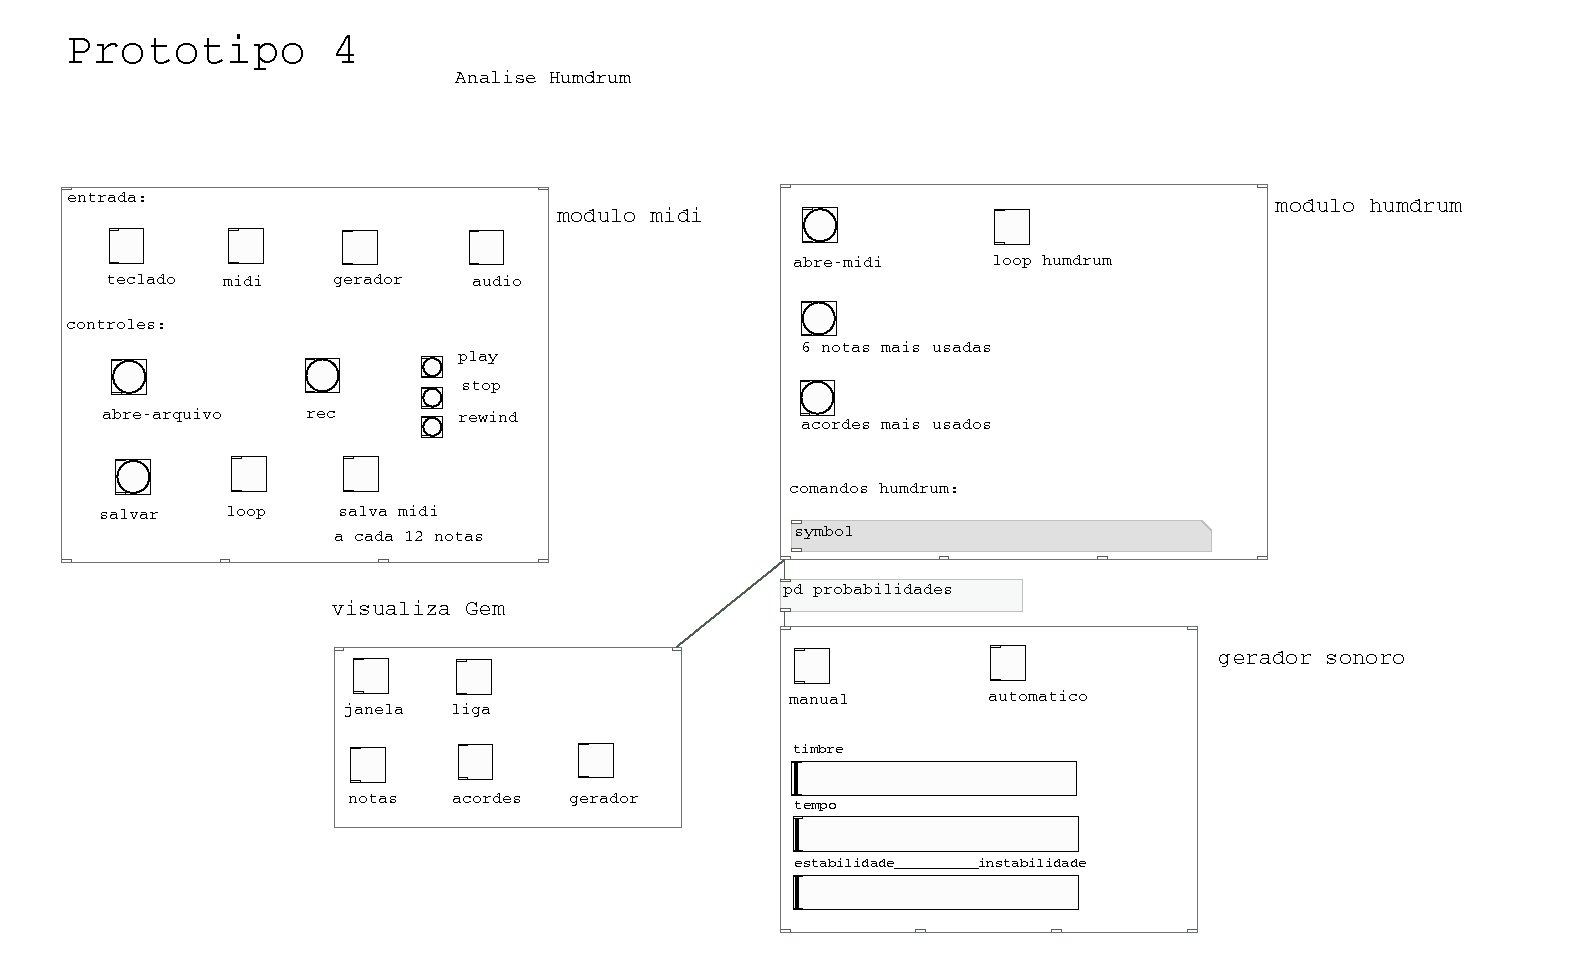
\includegraphics[scale=.5]{prot4}
% \caption{protótipo 4}
% \label{prot4}
% \end{figure}



\begin{figure}
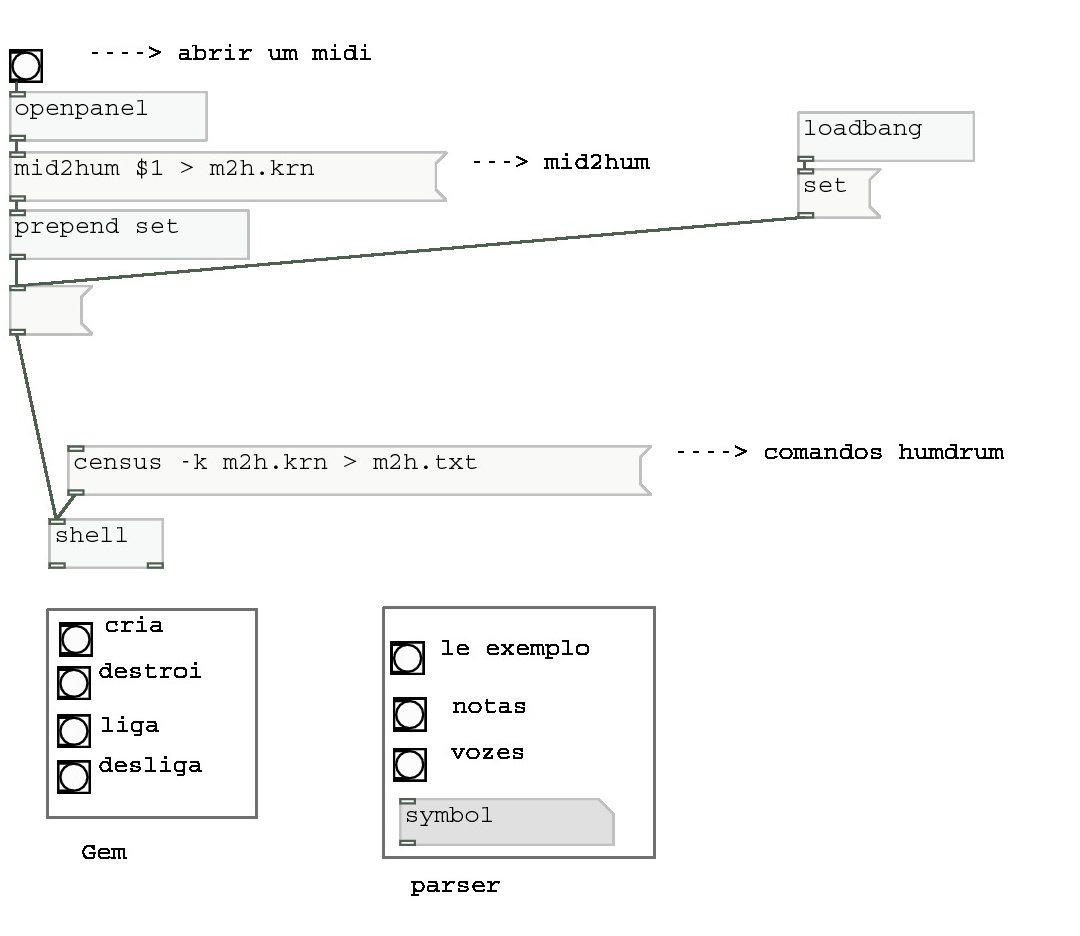
\includegraphics[scale=.7]{interface00}
\caption{interface}
\label{interface}
\end{figure} 

\textbf{Parseando strings no Pd}


O parser funciona em 3 instâncias:

1) Abre-se um arquivo midi com o objeto [openpanel] através
de uma janela de diálogo, o path do arquivo substitui a variável 
dólar 1 como argumento para o programa mid2hum que converte
arquivos midi para o formato kern (.krn), usado pelo humdrum.
\begin{verbatim}
 midi2hum \$1 > m2h.krn
\end{verbatim} 
  O código acima é formatado numa mensagem e enviado ao objeto
[shell] onde converte o arquivo midi e envia o resultado para
um novo arquivo chamado m2h.krn.
 
2) Nessa etapa é onde se aplica os comandos do humdrum ao 
arquivo gerado. No caso o comando
\begin{verbatim}
census -k m2h.krn > m2h.txt
\end{verbatim} 
traz diversas informações sobre o arquivo enviadas para um 
arquivo de texto como por exemplo:
\begin{verbatim}
 HUMDRUM DATA

Number of data tokens:     2510
Number of null tokens:     0
Number of multiple-stops:  470
Number of data records:    2511
Number of comments:        817
Number of interpretations: 301
Number of records:         3629

KERN DATA

Number of note-heads:      2491
Number of notes:           2209
Longest note:              2
Shortest note:             384
Highest note:              gggg#
Lowest note:               FFF
Number of rests:           310
Maximum number of voices:  4
Number of single barlines: 237
Number of double barlines: 0
\end{verbatim} 

3) Nessa parte expomos um método de navegar e procurar por
informações no arquivo de texto. O código usado como modelo,
está assinalado na figura \ref{parser}. O arquivo m2h.txt
é lido pelo objeto [msgfile] e envia uma lista com todo conteúdo
do arquivo para os objetos [list-find] e [list-seek]. Em [list-find]
podemos procurar por um símbolo específico dentro da lista e nos retorna
a posição do símbolo. No caso do código assinalado, vemos o símbolo 
``notes:'' , porém como desejamos o valor de ``notes:'' pegamos a posição
de ``notes:'' na lista e adicionamos um número para acessar o lugar do valor de
``notes:'' na lista. Essa posição é enviada para [list-seek] que retorna o valor ou
símbolo na posição desejada. Como teste escolhemos os parâmetros ``notes:'' e ``voices:'', 
respectivamente número de notas e número de vozes encontradas no arquivo.


\begin{figure}
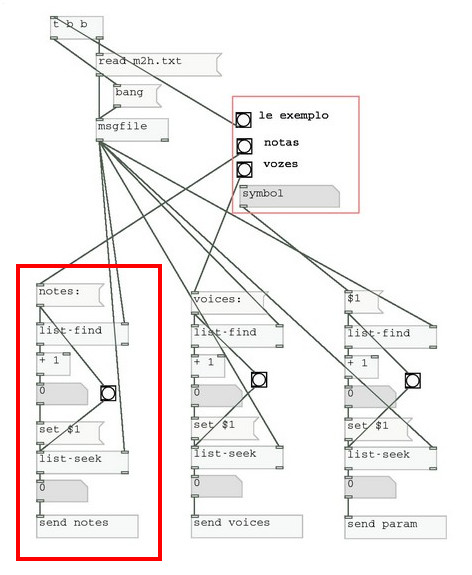
\includegraphics[scale=.5]{parser00}
\caption{parser}
\label{parser}
\end{figure} 


\textbf{Visualização com GEM}


  Os valores de números de notas e número de vozes são visualizados
com objetos da biblioteca Gem (Graphics Environment for Multimedia).
No caso os 2 parâmetros são enviados para 2 cubos 3D onde os valores
são lidos como valores de tamanho dos cubos.



\begin{figure}
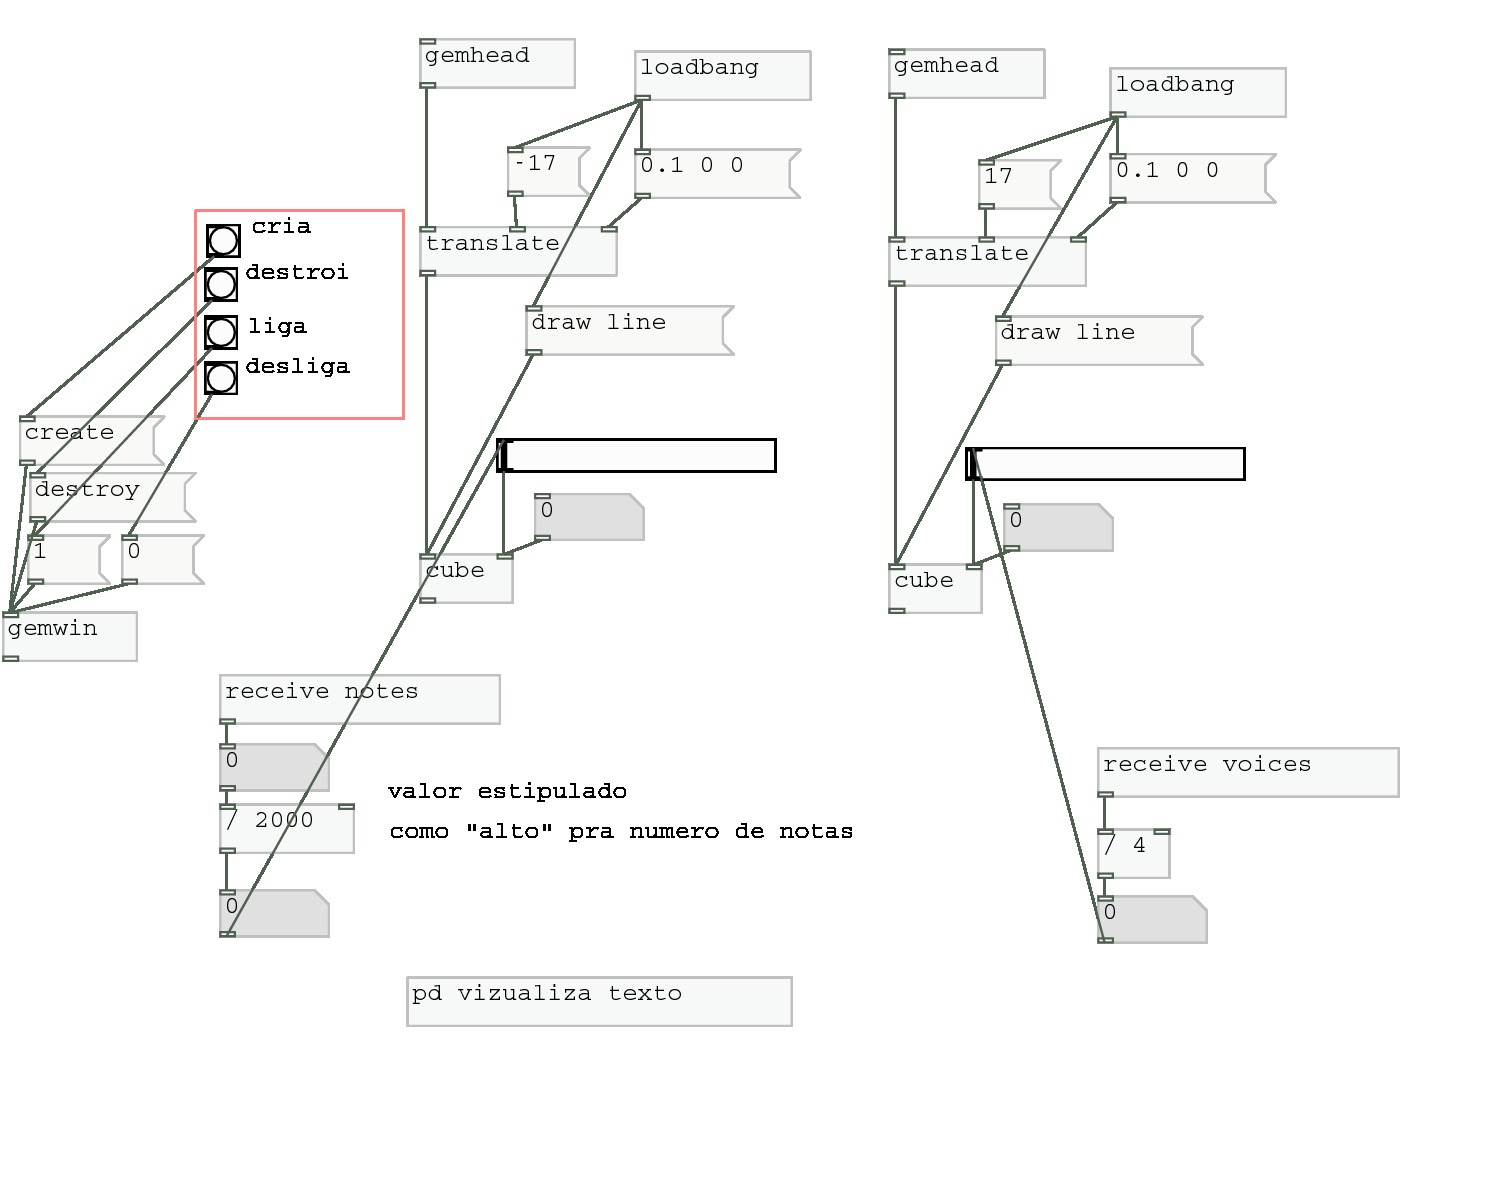
\includegraphics[scale=.5]{gem00}
\caption{GEM}
\label{GEM}
\end{figure} 


\begin{figure}
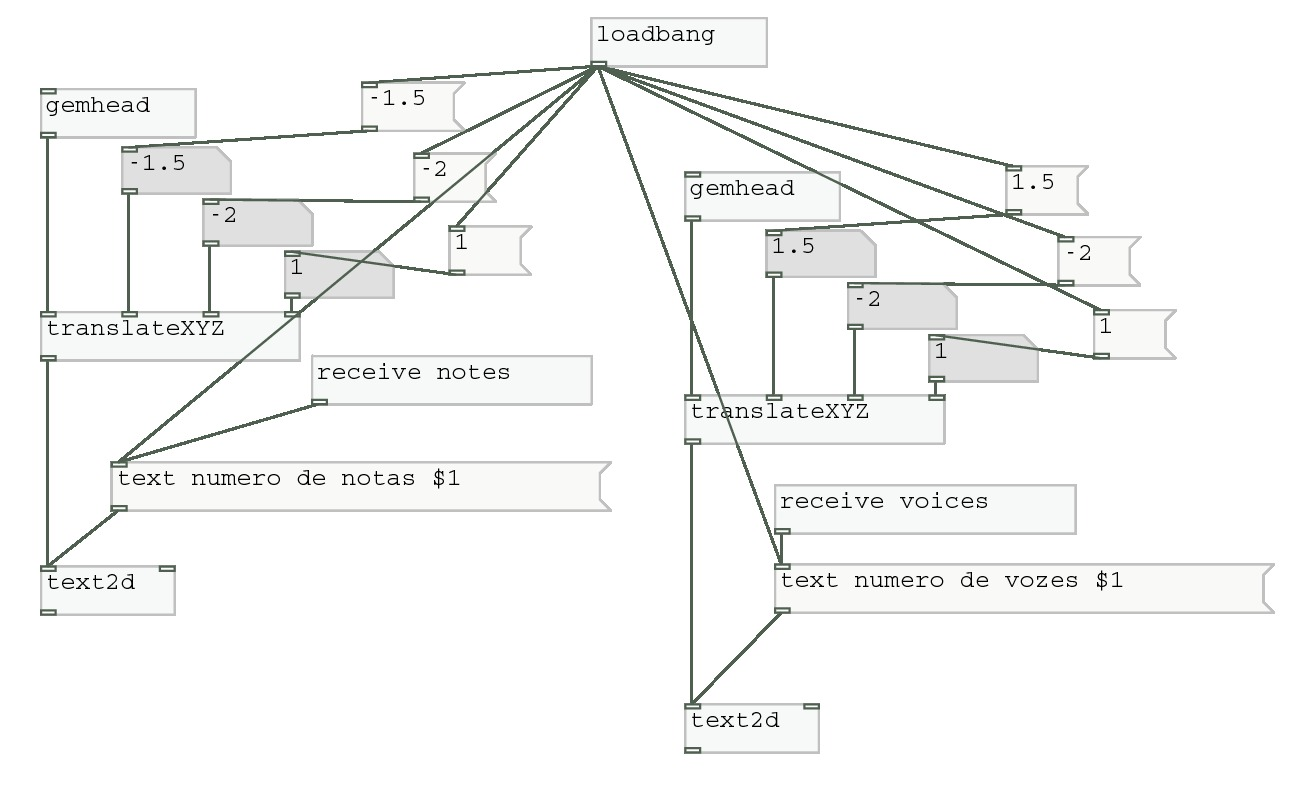
\includegraphics[scale=.5]{gemtexto00}
\caption{GEM texto}
\label{GEM texto}
\end{figure} 



\begin{figure}
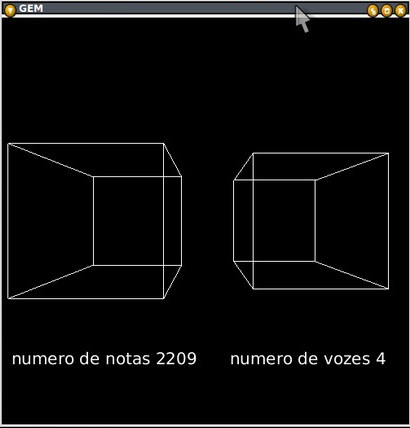
\includegraphics[scale=.5]{gemwin}
\caption{gemwin}
\label{gemwin}
\end{figure} 



  Nesse protótipo, mostramos uma metodologia
simples de unir duas linguagens muito usadas em pesquisa de música.
Essa metodologia é uma maneira clara de como acessar outra linguagem dentro do Pd
enriquecendo as possibilidades da linguagem.


\pagebreak





\section{Geradores MIDI}

%% em primeiro lugar dizer  O QUE SÃO OS GERADORES

Nessa seção serão descritos os geradores MIDI, que
são módulos de composição algorítmica alimentados
por dados da análise da entrada do músico.

Durante a implementação dos geradores de material musical,
procurou-se aliar técnicas de composição algorítmica com
o resultado das análises do áudio de entrada.


A idéia de ter uma coleção de geradores, capazes
de imitar elementos da performance humana. A análise do áudio
tenta fazer uma descrição da performance e essa descrição
é enviada aos geradores, mediados pelo cenário de interação.
Nesse sentido as análises alimentam os parâmetros dos
geradores, conduzindo o comportamento dos mesmos.



Notadamente alguns trabalhos tem influenciado bastante o desenvolvimento
dos geradores, servindo de ponto de partida para a implementação. Como
por exemplo a biblioteca RTC\footnote{A biblioteca RTC (\textit{Real-Time Composition} 
foi desenvolvida pelo compositor Karlheinz Essl em MAX, a re-implementação
em Pd foi feita por Frank Barchnet, poderemos ver uma visão mais geral
das funcionalidades dessa biblioteca no apêndice} e o método MEPSOM\footnote{
MEPSOM (Método de Ensino de Programação Sônica para Músicos) desenvolvido por
Elói Fritsch é um método que ensina composição algorítmica no ambiente MAX. Alguns
exemplos de MEPSOM foram portados para Pd e podem ser vistos no apêndice}, além
de alguns objetos das bibliotecas PDMTL e Rj.  


Músicos frequentemente separam os aspectos rítmicos, melódicos e de dinâmica
quando estudam performance ou compõe. É comum um instrumentista executar um 
mesmo perfil melódico em diferentes combinações rítmicas e com articulações
diferentes. Muitos métodos de educação musical começam com exercícios rítmicos
para depois incluir exercícios melódicos. Ao implementar os geradores midi
nessa pesquisa, levou-se em conta esses aspectos e decidiu-se manter a separação
entre os domínios do ritmo, melodia e dinâmica. Criando uma relação de funcionamento
desses geradores, possibilitando uma expansão organizada de técnicas de geração.
Na implementação de Sincopa, projetamos 3 objetos que trabalham juntos para
gerar dados midi: 

\begin{itemize}
 \item   [sinc-gera-ritmico]
 \item   [sinc-gera-melodico]
 \item   [sinc-gera-dinamica]
\end{itemize}

Cada um desses objetos gerencia algumas técnicas de geração
algorítmica. É possível qualquer combinação entre esses três objetos.
A combinação entre os diversos geradores se dá na relação entre a 
análise do áudio de entrada e a escolha de um cenário de interação. 

A manipulação de dados midi compreende algumas técnicas bem estabelecidas
no Pd. A geração de notas midi é realizada com o objeto [makenote] que formata
dados de entrada em notas midi, fornecendo as mensagens "noteon" e "noteoff", baseado
no valor de duração. As entradas e saídas midi são feitas com os objetos
[notein] e [noteout] respectivamente. O objeto [seq] grava e manipula arquivos 
do tipo midi, porém, os parâmetros das mensagens midi podem ser facilmente escritos
em arrays e listas para então serem manipulados.

\begin{figure}
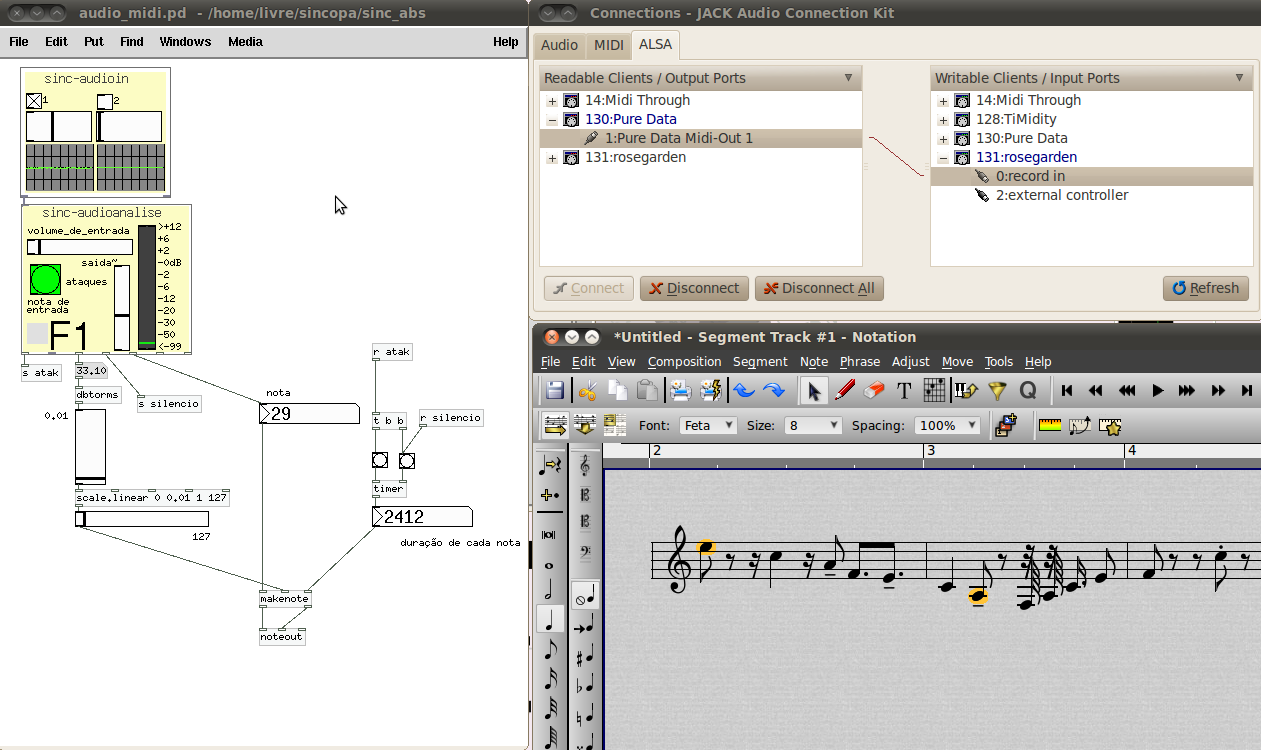
\includegraphics[scale=.5]{audio2midi}
\caption{Conversão de áudio para notas midi}
\label{audio2midi}
\end{figure}


Na figura \ref{audio2midi} vemos no patch a esquerda, o fluxo de entrada de áudio do objeto
[sinc-audioin], sendo analisado pelo objeto [sinc-audioanalise] e posteriormente
sendo convertido para mensagens midi com auxílio dos objetos [makenote] e [noteout].
Podemos observar ainda a dinâmica sendo convertida de decibéis (distribuição exponencial)
 para RMS (distribuição linear) com o objeto [dbtorms]. Após essa conversão,
o valor da dinâmica é convertido para uma escala midi de 0 a 127. Para isso é usado
o objeto [scale.linear] da biblioteca "pdmtl". O valor de duração das notas é determinado
pelo objeto [timer] que recebe uma mensagem (bang) a cada detecção de ataque e de silêncio.
No panorama geral da figura\ref{audio2midi} vemos o Pd mandando mensagens midi em tempo-real
para o programa Rosegarden, usando conexão midi do programa Jack. 


\subsection{Manipulação e escrita de dados MIDI}

% Explicar rapidamente como entram dados MIDI, como se estocam, analizam e explicar uma
% abstração simples que contenha esses elementos.
% 
% Objetivo da abstração: salvar o midi com a entrada e o gerador em um arquivo .midi

\begin{figure}
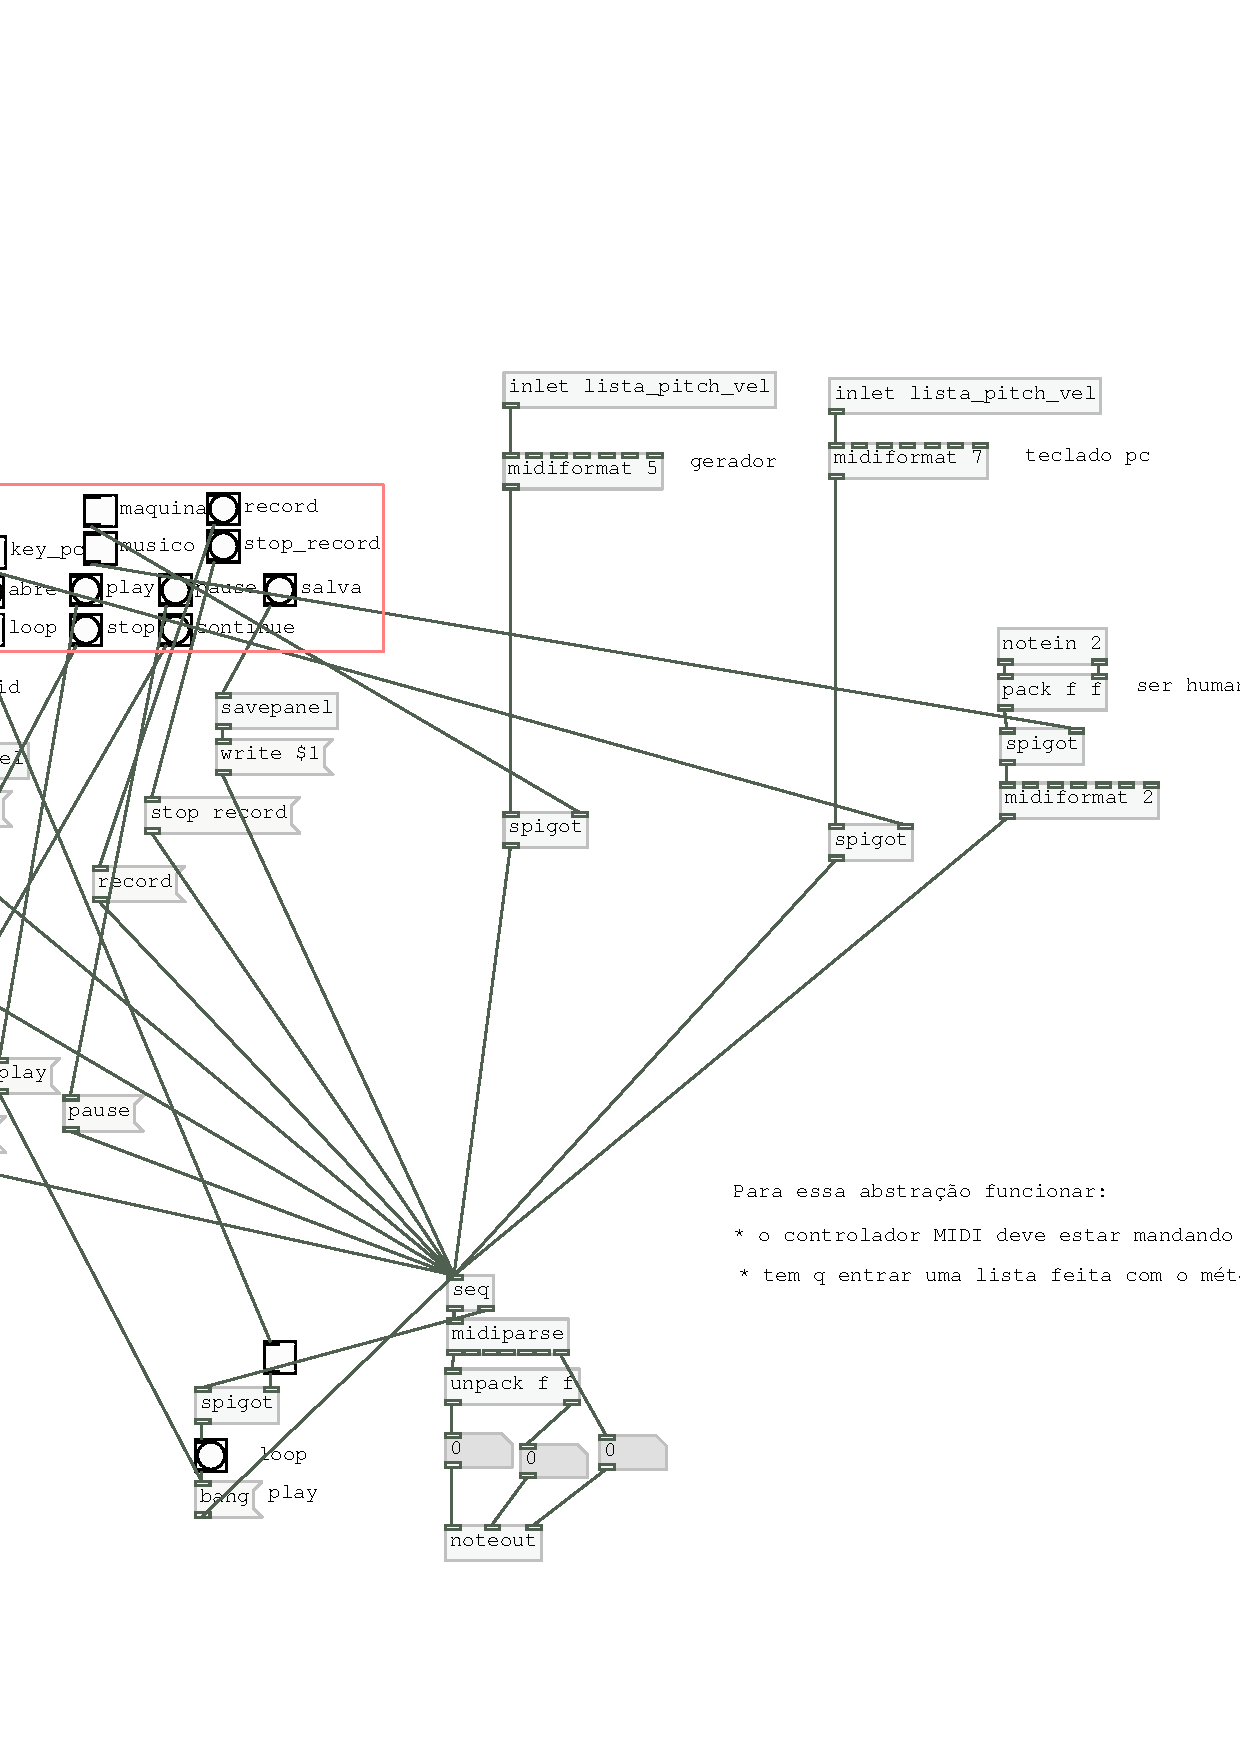
\includegraphics[scale=.5]{sinc-midiin}
\caption{Objeto [sinc-midiin]}
\label{sinc-midiin}
\end{figure}


\begin{figure}
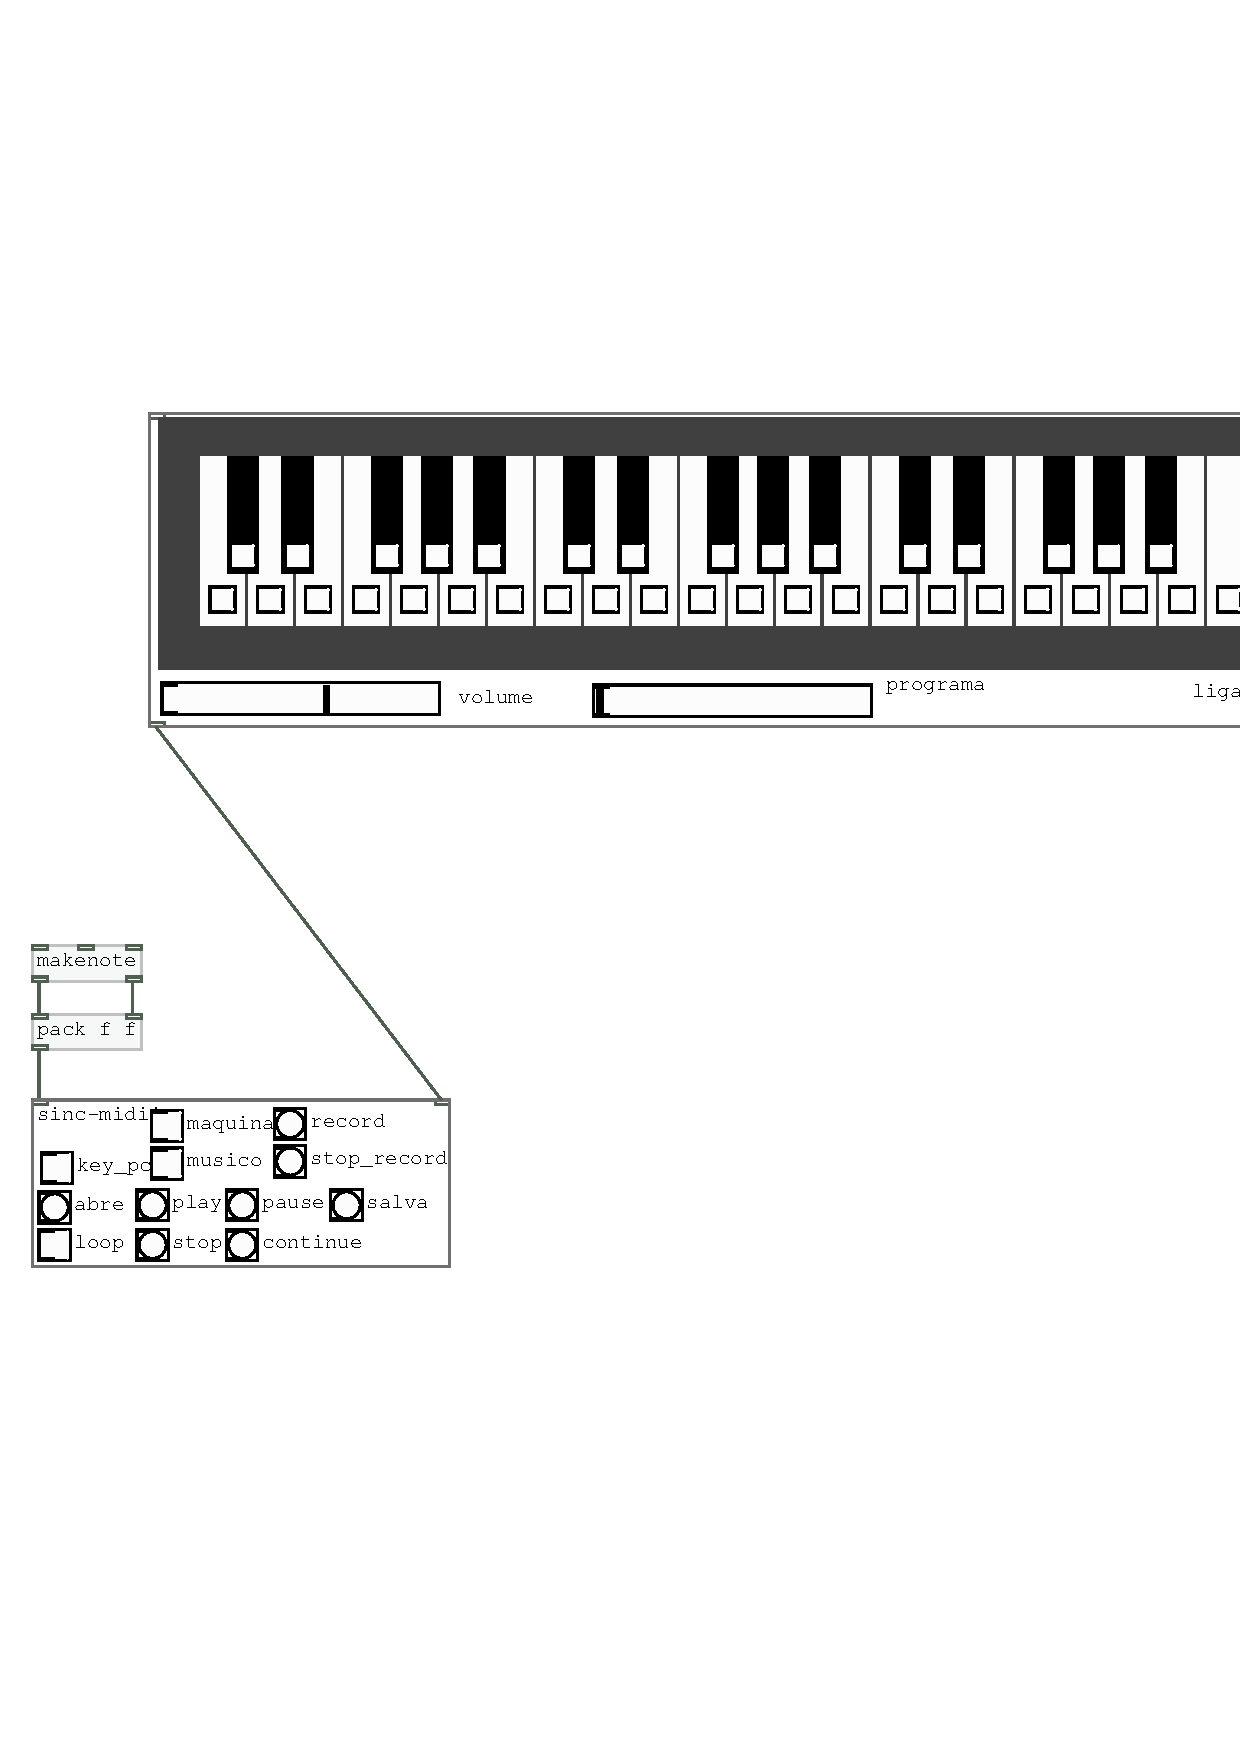
\includegraphics[scale=.5]{sinc-midiin-help}
\caption{Exemplo de funcionamento de [sinc-midiin]}
\label{sinc-midiin-help}
\end{figure}


Foi desenvolvida uma abstração que facilita a leitura e escrita dos dados MIDI. É baseada no
objeto [seq].

* Definição de um padrão de distribuição de canais midi.

* o MIDI pode ser usado tanto em situações de gravação e repetição ou
transformação em tempo-real, quanto como registro de uma sessão de interação.
Nesse caso, pode ser editado posteriormente em notação musical, como pode ser
visto na seção \ref{sec-notacao} onde pode s


\subsection{Geradores rítmicos}






\begin{figure}
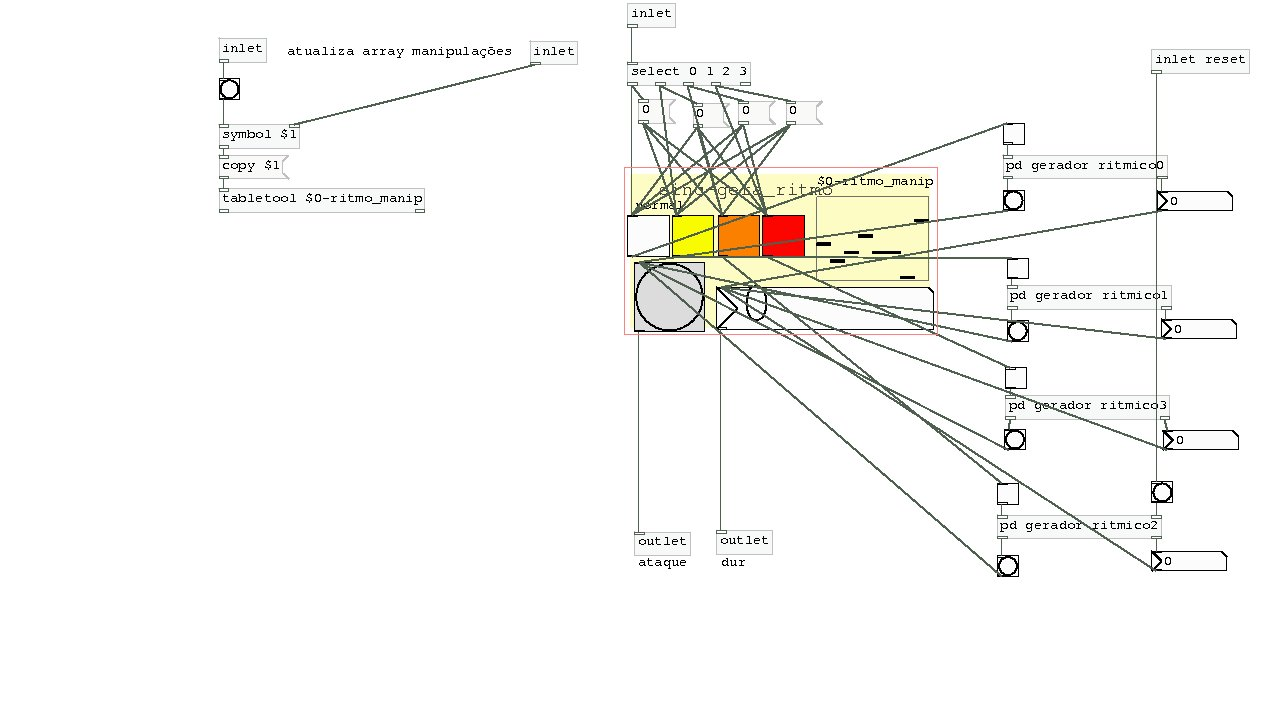
\includegraphics[scale=.5]{sinc-gera-ritmo}
\caption{Objeto [sinc-gera-ritmico]}
\label{[sinc-gera-ritmico]}
\end{figure}

No atual estágio da pesquisa, foi implementada uma abstração gráfica
que gerencia a atividade de quatro geradores rítmicos. Dessa
maneira se torna fácil de administrar durante uma performance
e também se mantém a flexibilidade de expandir para quantos
geradores diferentes se queira. A interface pode ser vista na figura \ref{[sinc-gera-ritmico]}


\subsubsection{Gerador rítmico imitativo}



\begin{figure}
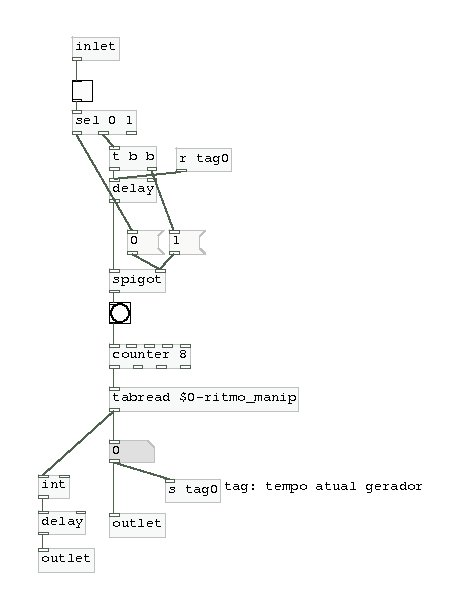
\includegraphics[scale=.6]{gerador-ritmico0}
\caption{subpatch [pd gerador-ritmico0] de [sinc-gera-ritmico]}
\label{gera-ritmico0}
\end{figure}   


No patch da figura \ref{gera-ritmico0} vemos um gerador de



% \item
 \subsubsection{Ritmo baseado em variações}


Na figura \ref{gera-ritmico1} vemos um gerador rítmico
que compõe novas sequências rítmicas a partir de variações
da tabela de durações.

Essas variações podem ser:

\begin{figure}
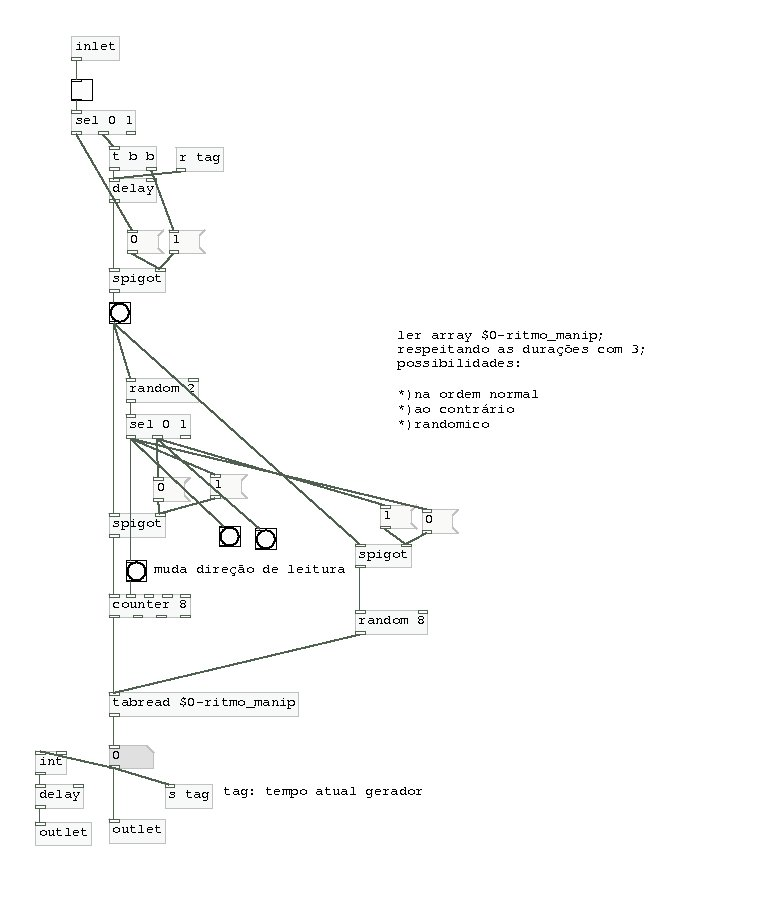
\includegraphics[scale=.6]{gerador-ritmico1}
\caption{Gerador rítmico baseado em probabilidades de durações}
\label{gera-ritmico1}
\end{figure}  




% \item
 \subsubsection{Movimento browniano como gerador de durações}


\begin{figure}
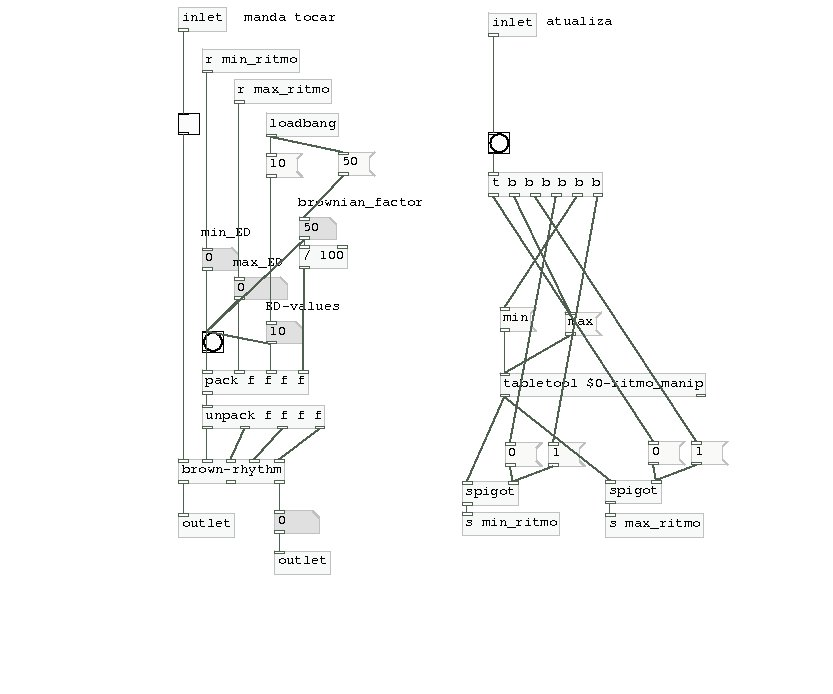
\includegraphics[scale=.6]{gerador-ritmico2}
\caption{Gerador rítmico baseado em movimento browniano}
\label{gera-ritmico2}
\end{figure}  


O terceiro gerador é mostrado na figura \ref{gera-ritmico2} e
realiza uma combinação entre os objetos [tabletool] e [brown-rhythm].

O objeto [tabletool]\footnote{Objeto externo desenvolvido em C
por William Brent e compilado e testado no ambiente de desenvolvimento
dessa pesquisa} permite que se façam operações matemáticas
recursivas e análise em arrays de números. 

Nesse caso, [tabletool] é responsável por informar os valores
mínimo e máximo de durações de tempo entre notas, que estão
armazenados no array \textit{\$0-ritmo-manip}, enviando
esses respectivos valores como variáveis [s min-ritmo] e 
[s max-ritmo] para o gerador de durações [brow-rythm].


 \begin{figure}
\includegraphics[scale=.6]{brown-rythm}
\caption{brow-rythm}
\label{brown-rythm}
\end{figure}  

O objeto [brown-rhythm] está presente na biblioteca RTC e se trata de
um gerador de durações baseado em movimento browniano("Brown motion"
\footnote{movimento browniano é um modelo que descreve o movimento aleatório 
de partículas macroscópicas num fluido como consequência dos choques das 
moléculas do fluido nas partículas. Esse nome é devido ao botânico Robert
Brown, que observou minúsculas partículas dentro dos vacúolos dos grãos de 
pólen executando um movimento agitado. Repetindo o experimento com partículas de poeira, 
ele foi capaz de definir que o movimento se deu devido às partículas estarem "vivas", 
embora a origem do movimento ainda estivesse para ser explicada.
O cientista que explicou corretamente esse movimento, propondo que a energia fosse 
constituída de partículas, foi Albert Einstein, em 1905.
Movimento browniano é um dos modelos mais usados de processos estocásticos
(ou probabilísticos) sobre tempo contínuo.} )

 \begin{figure}
\includegraphics[scale=.6]{brown-rhythm-func}
\caption{Funcionamento básico de [brow-rhythm]}
\label{brown-rythm-func}
\end{figure} 


O funcionamento básico aparece na figura \ref{brown-rhythm-func}.
No manual de [brown-rhythm] aparece uma explicação mais detalhada.


\begin{quote}
Generates a brownian-movement-like rhythm of a geometrical row of
entry delays (ED) and a certain number of ED-values. The brownian factor
determines the distance between two succeding rhythmical values. A factor
of 0 produces a periodic rhythm, where a factor of 1 output random values 
of the given range.
\end{quote}  



Na figura \ref{brown-rythm} vemos como [brown-rythm] é construído internamente.
Nota-se em destaque os principais objetos envolvidos na construção
de [brown-rhythm]. Basicamente, o objeto [brownian] é uma implementação de
distribuição de Brown no Pd. E [trans-log] é um objeto que realiza uma
transição logarítmica entre números.

 \begin{figure}
\includegraphics[scale=.6]{brownian-func}
\caption{Funcionamento de [brownian]}
\label{brownian-func}
\end{figure} 

Podemos ver o funcionamento básico do objeto [brownian] acessando seu
manual (figura \ref{brownian-func}.  A saída desse objeto retorna números randômicos entre o mínimo
(''min'' (int, float)) e o máximo (''max" (int, float)). A distância entre
dois números randômicos é determinada pelo fator de brown (float
entre 0 e 1). Quando esse fator é 1, [brownian] se comporta como um
gerador randômico ordinário (objeto [random] por exemplo). Quando
o fator é 0, o mesmo número sempre é repetido.


\begin{figure}
\includegraphics[scale=.6]{brownian-exemplo}
\caption{objeto [brownian] com diferentes valores de fator de brown}
\label{brownian-exemplo}
\end{figure} 

É possível comparar diferentes comportamentos de [brownian] observando
a figura \ref{brownian-exemplo}, onde vemos três objetos [brownian] com
os mesmos parâmetros de inicialização, cada um escrevendo os resultados
em diferentes arrays de 50 elementos. A única diferença entre os 3 está 
no fator de brown, assinalado em rosa (0.01 , 0.1 e 0.5 respectivamente).
Musicalmente, um baixo fator de brown aplicado a durações entre notas
possibilita a emergência de padrões rítmicos bem estabelecidos com 
pequenas variações. Quando aumentamos gradualmente o fator de brown, ouvimos
uma transição rumo a uma instabilidade rítmica e a quebra de padrões. 
O objetivo desse gerador é se aproximar da performance do músico real.
O objeto [sinc-audioanalise] analise o áudio de entrada estimando os valores de duração entre notas.
Esse valores são enviados a [sinc-calc-ritmo] que faz uma estimativa do grau
de instabilidade, como explicado na página \ref{[sinc-calc-ritmo]} (como faz pra ref a página?).
O grau de instabilidade rítmica influencia direto o comportamento do fator de brown, de acordo
com a definição do cenário de interação a que se propõe. O cenário pode definir, por exemplo, que
um ritmo estável do músico (baixa instabilidade), provoque um comportamento rítmico instável
do gerador (fator de brown alto).



 \begin{figure}
\includegraphics[scale=.6]{brownian}
\caption{[brownian]}
\label{brownian}
\end{figure} 


Na figura \ref{brownian} vemos a composição interna do objeto [brownian] onde temos elementos
grifados com a cor verde e outros com a cor rosa. Se trata de duas partes
distintas do patch, a parte com a cor verde, representa o controle dos
parâmetros do objeto [drunk] que é a implementação de um modelo de \textit{random-walk}
no Pd. A área destacada em rosa mostra uma sequência de objetos que 
escalonam o resultado dentro da amplitude de valor mínimo (\$1) e máximo (\$2).

 \begin{figure}
\includegraphics[scale=.6]{drunk}
\caption{exemplo de funcionamento de [drunk]}
\label{drunk}
\end{figure} 

O objeto [drunk] pertence a biblioteca Cyclone, que tem como objetivo
implementar objetos compatíveis entre Pd e MAX. O objetivo de [drunk] é
retornar números randômicos dentro de uma escala variável. A distância
entre cada número randômico é definida pelo valor da terceira entrada
de [drunk]. Essa variável define o maior número de passos possível entre 
dois resultados de [drunk]. Podemos ver na figura \ref{drunk} que temos
dois objetos [drunk] sorteando 16 valores de 0 a 10 com a diferença do
número de passos, com 6 (destaque em verde) e 2 (destaque em rosa).

Os objetos [brownian] e [drunk] são muito úteis para a composição 
interativa por permitirem a variação dos parâmetros do algoritmo
em tempo-real. Essa funcionalidade é usada em SINCOPA em outros geradores
melódicos e de dinâmica.


%  \item
\subsubsection{Gerador rítmico polifônico}


\begin{figure}
\includegraphics[scale=.6]{gerador-ritmico3}
\caption{Gerador rítmico randômico}
\label{gera-ritmico3}
\end{figure}  

O gerador da figura \ref{gera-ritmico3} é baseado no 
objeto [repchord-rhythm] da biblioteca RTC. O objetivo desse objeto é 
ter um gerador com capacidade de controle dos parâmetros da polifonia.

O objeto [repchord-rhythm] é um gerador rítmico polifônico cujas taxa repetição
e densidade do acorde são dependentes dos graus de periodicidade de durações
mínima e máxima entre notas. 
%\end{itemize}


\subsection{Geradores melódicos}


Da mesma maneira que os geradores rítmicos.....
No atual estágio da pesquisa, foi implementada uma abstração gráfica
que gerencia a atividade de quatro geradores melódicos. Dessa
maneira se torna fácil de administrar durante uma performance.
E também se mantém a flexibilidade de expandir para quantos
geradores diferentes se queira.


De maneira geral, os geradores melódicos dependem dos geradores
rítmicos. Os geradores rítmicos "pedem" nota por nota para o geradores
melódicos


\begin{figure}
\includegraphics[scale=.45]{sinc-gera-melodico}
\caption{Abstração que organiza 4 geradores melódicos}
\label{[sinc-gera-melodico]}
\end{figure}


\subsubsection{Melodia imitativa}

Nesse primeiro gerador melódico o método de geração
é a leitura linear da tabela temporária de pitches
como se pode ver na figura \ref{gera-melodico0}.


\begin{figure}
\includegraphics[scale=.6]{gera-melodico0}
\caption{[pd gerador-melodico0]}
\label{gera-melodico0}
\end{figure}  

\begin{figure}
\includegraphics[scale=.55]{gera-mel0}
\caption{exemplo de melodia imitativa gerada}
\label{gera-mel0}
\end{figure}  




O objetivo desse gerador é a imitação melódica
do instrumentista.

\subsubsection{Melodia de probabilidades}



Nesse objeto foi implementada uma probabilidade unidimensional
de durações. Ou seja, o valor absoluto de cada duração
da performance do músico alimenta uma tabela de durações.
Uma possível aplicação seria a aplicação de probabilidades de 
padrões maiores de durações. Permitindo a recorrência dos padrões
rítmicos que emergem ao longo da performance.


No Pd podemos implementar um sistema simples de probabilidade como 
vemos na figura XXX

% fazer exemplo simples de probabilidade genérica - patch simples



O objeto [probalizer], simplifica o trabalho.

Importância das probabilidades serem atualizadas em
tempo-real.

Explicar patch simples de probabilidade e como
seria a re-implementação do probalizer apenas com vanilla.


O gerador melódico da figura \ref{gera-melodico1}, é baseado
no objeto gráfico [probalizer] da biblioteca "Unauthorized"
distribuída com o pd-extended.

O objeto [probalizer], facilita o trabalho.

Importância das probabilidades serem atualizadas em
tempo-real.
Explicar probabilidade simples.

\begin{figure}
\includegraphics[scale=.6]{gera-melodico1}
\caption{[pd gerador-melodico1]}
\label{gera-melodico1}
\end{figure}  

\subsubsection{Movimento browniano como gerador melódico}


\begin{figure}
\includegraphics[scale=.6]{gera-melodico2}
\caption{[pd gerador-melodico2]}
\label{gera-melodico2}
\end{figure}  


O terceiro gerador é mostrado na figura \ref{gera-melodico2} e
realiza uma combinação entre os objetos [tabletool] e [brown-melody].


\subsubsection{Melodia  de notas randômicas}


\begin{figure}
\includegraphics[scale=.6]{gera-melodico3}
\caption{[pd gerador-melodico3]}
\label{gera-melodico3}
\end{figure}  

O gerador da figura \ref{gera-melodico3} é baseado no 
objeto [random.integer]. O objetivo desse gerador é 
ter um gerador com alto grau de permeabilidade melódica.

\subsection{Geradores de amplitudes}

São encontrados diferentes termos definindo o aspecto
da amplitude sonora como dinâmica (quando nos referimos a notação tradicional),
velocity (quando se refere a dados MIDI), volume e amplitude (mais
usado quando se refere a descrição física da onda sonora).


As variações de amplitude podem produzir diferentes gestos musicais,
Gerando acentos, diferentes articulações...


\subsubsection{Amplitude imitativa}

bla bla bla

\subsubsection{Gerador de amplitude baseado em variação}


\subsubsection{Movimento browniano como gerador de amplitude}


\subsubsection{Amplitude polifônica}

conceito de orquestração

\subsection{Harmonizador automático}


Essa seção tem como objetivo apresentar possibilidades de harmonização automática em tempo-real.
Onde o sistema tendo o conhecimento da linha melódica criada instantaneamente pelo músico, consegue
harmonizar essa linha melódica.

Uma extensa bibliografia tem sido desenvolvida nos últimos 30 anos sobre o tema da harmonização automática.
Muitas empresas subsidiam a pesquisa nesse tema com o objetivo de produzir produtos comerciais que realizem
harmonização automática de maneira satisfatória para o usuário final. Esse processo vem acumulando patentes
de algoritmos de harmonização por parte de companhias fabricantes de teclados e desenvolvedoras de programas comerciais
de produção musical. Um exemplo é o programa ``Band-in-a-Box'' que realiza harmonizações de acordo com
a análise prévia de estilos. Nesse caso a harmonização não é feita em tempo-real e tem como finalidade
o exercício musical caseiro de criação melódica sobre harmonizações de diferentes estilos.
Outro exemplo são as harmonizações automáticas de teclados comerciais populares, onde o usuário escolhe
a tonalidade manualmente e um programa interno realiza uma harmonização tonal, simples, mas muitas vezes 
satisfatória para certos estilos de música.

%% colocar na bibliografia os pdf's em ~/cristiano-doutorado/mat_tese/biblio_harmoniza

Ching-Hua Chuan define em sua tese, um sistema de harmonização que leva em conta parâmetros
de análise de cada nota presente em um fluxo melódico, como duração, duração das notas anteriores, número
de ocorrências de determinado pitch class ao longo da melodia, direcionalide melódica e diversos outros
parâmetros. Por fim, expõe um modelo de acompanhamento harmônico e obtém um resultado positivo ao apresentar
o sistema acompanhando canções populares.

Matt Hanlon e Tim Ledlie apresentam um sistema de harmonização de corais a quatro vozes no estilo de Bach.
A composição da progressão harmônica é implementada com um modelo estatístico de cadeias de Markov
(Hidden Markov Model), e deriva na solução da harmonia através da solução de problemas
de satisfação restrita (constraint satisfaction problem).Após
essa etapa é feita a realização da progressão em linhas melódicas para quatro vozes

Uma implementação bem detalhada de um harmonizador automático que faz uso de
 regras de harmonia tradicional é descrita na patente Norte-Americana 
US 7,189,914 B2  assinada por Allan John Mack. O harmonizador inicia
na primeira nota da melodia e de acordo com a escala e modo providos
pelo usuário, o sistema escolhe uma especificação de acorde dentre
as especificações estocadas em memória, que podem ser definidas pelo usuário
e são estocadas em arrays lidos pelo programa em tempo-real.
Nessa implementação, uma série enorme de regras de sequência harmônica e 
condução de vozes são definidas baseadas em regras comuns a diversos cursos
de harmonia tradicional, como evitar 5ªs e 8ªs paralelas e progressões
``proibidas'' (I - ii - iii , por exemplo).

Um aspecto complexo das regras de harmonia tradicional é que as regras
de condução das vozes se misturam de forma iterativa com as regras de
progressão harmônica. Na descrição da patente, o autor exibe trechos do sistema em pseudo-código,
mostrando a maneira como a sequência harmônica influencia na condução vocal e vice-versa,
e o nível de detalhamento do projeto:

\begin{verbatim}
VI to V progression
if the preceding and current chords are at their root positions then
  if the preceding chord is of dominant root then
    if the preceding chord is a triad in a minor key or a seventh in a 
      major key then
      if the current chord is a submediant triad then
	if the preceding chord has no seventh and no fifth then rule 361 fails
	if the third of the current chord has no double then rule 386 fails
      end if
    end if
   else if the current chord is a dominant triad then
    if the previous chord is a submediant triad in a minor key then
      if the current chord has no fifth then rule 361 fails
      if the third of the previous chord has no double then rule 386 fails
    end if
  end if
end if
\end{verbatim}

Dentro do escopo de SInCoPA, foram desenvolvidos alguns métodos de harmonização
melódica para uso composicional.
Pode-se pensar em relações não-usuais de parâmetros
como amplitude e densidade rítmica como controladores de 
comportamento de harmonizadores. 
Um dos objetivos é a flexibilidade e modularidade da implementação
de harmonizadores que possibilite novas relações e ``regras'' de
interação do músico humano com a dimensão harmônica da
composição. 


\subsubsection{Nota pertence ao acorde}

%% antigo::

Nessa técnica foi definido que a maior exigência será que o acorde contenha a nota que está sendo
tocada pelo músico e harmonizada pelo computador. 
Para isso são expostas 2 possibilidades de harmonização automática, com resultados distintos.

No patch da figura \ref{harm1}  temos a célula básica do harmonizador diatônico 
 usado no protótipo. 
O objeto [receive fiddle] recebe o fluxo de notas e o objeto [decide], escolhe 
randomicamente quais notas vão ser harmonizadas, e manda sua decisão para o objeto 
[spigot] que funciona como uma chave seletora liberando ou não a nota para ser harmonizada. 
Após a nota ser liberada para o harmonizador, vai acontecer  a escolha de qual acorde será 
sobreposto a essa nota. Isso é feito pelo objeto [random 4] que escolhe randomicamente um 
número de 0 a 3, cada um representando uma operação a ser feita com a nota dada pela flauta 
(ver ainda na figura \ref{harm1} - ``tabela de resultados de [random 4]'').

\begin{figure}
\includegraphics[scale=.6]{harm1}
\caption{Decisão de qual nota a ser harmonizada}
\label{harm1}
\end{figure}

\begin{figure}
\includegraphics[scale=.6]{harm2}
\caption{sub-patch ``pd tonica''}
\label{harm2}
\end{figure}

\begin{figure}
\includegraphics[scale=.4]{harm3}
\caption{resultado da harmonização com modo 1}
\label{harm3}
\end{figure}


Na figura \ref{harm2} podemos ver o que acontece dentro do sub-patch [pd tônica], onde a nota sorteada 
será a tônica de uma tríade maior ou menor dependendo do resultado de [random 2]. A figura \ref{harm3} 
mostra um pequeno exemplo dos resultados desse harmonizador. Nesse exemplo, a primeira nota 
harmonizada é um si que virou terça maior de uma tríade maior. Um aspecto interessante desse 
harmonizador é que mesmo em exemplos curtos quase sempre se chega a relações de mediantes 
cromáticas, como é o caso do terceiro e quarto acordes (Mib - Lab), nesse caso uma relação 
enarmônica de mediante cromática.

\begin{figure}
\includegraphics[scale=.5]{harm4}
\caption{harmonizador dissonante , modo 2}
\label{harm4}
\end{figure}

Apesar de muitas vezes os acordes gerados pelo harmonizador diatônico possuírem uma relação 
cromática, todos os acordes gerados são tríades maiores ou menores. Para criar um contraste 
foi criado um harmonizador de acordes alterados que está na figura \ref{harm4}. Nesse harmonizador todas notas 
que entram são tônicas e todas são harmonizadas. 
	A escolha do acorde para cada nota é feito através de distribuição de probabilidade, 
arranjado com o objeto [moses]. Quando uma nota entra, ela gera randomicamente um número de 0 
a 99 com o objeto [random 100], esse valor então é endereçado a um dos quatro tipos de tétrades 
possíveis nesse patch : aumentado com 7ª menor, alterado com 5ª diminuta (6ª aumentada Francês), 
menor com sétima maior ou maior com sétima maior. Cada uma das quatro tétrades tem 25 por cento 
de probabilidade de aparecer. Cada membro dos acordes é endereçado a um gerador de síntese aditiva 
com amplitude bem baixa. Em função da amplitude bem baixa do harmonizador de acordes alterados, o 
resultado funciona bem como uma textura dissonante .

% ainda falar dos modos 3 e 4 

%O presente trabalho é produto da fase inicial de investigação de minha pesquisa de doutorado. 

\begin{figure}
\includegraphics[scale=.4]{harm5}
\caption{pd, jack e rosegarden}
\label{harm5}
\end{figure}

O objetivo é a investigação de possibilidades e prototipação de estruturas computacionais com 
objetivo de agregar interatividade ao trabalho composicional.  
	Apesar desses harmonizadores terem sido usados nessa peça para interação com áudio em 
tempo-real, podem ser muito úteis como geradores de material escrito em notação tradicional, 
como mostra a figura \ref{harm5}. Esta imagem mostra o patch de Pd mandando as informações para o programa 
de notação Rosegarden através do programa Jack que funciona como um servidor de comunicação entre 
programas.Esse tipo de operação possibilita uma usabilidade do Pd semelhante ao programa Open-music 
do Ircam.


\subsubsection{Acorde pertence a coleção de notas}

\begin{figure}
\includegraphics[scale=.4]{harm-colecao}
\caption{Resultado de harmonizador automático com acordes pertecentes a coleção de notas tocadas}
\label{harm-colecao}
\end{figure}

\begin{figure}
\includegraphics[scale=.4]{harm6}
\caption{Patch que harmoniza de acordo com as notas executadas pelo músico estocadas em um array}
\label{harm6}
\end{figure}

Nesse patch é implementado um harmonizador simples,onde a sequência dos acordes e
a condução vocal é totalmente randômica. A única regra é que as notas usadas na composição
dos acordes tenham sido tocadas pelo músico.

\subsubsection{Sequência baseada em regras}

% \begin{figure}
% \includegraphics[scale=.4]{harm6}
% \caption{Patch que harmoniza de acordo com as notas executadas pelo músico estocadas em um array}
% \label{harm6}
% \end{figure}
% fazer a imagem baseada em [sinc-chordseq]

\begin{figure}
\includegraphics[scale=.4]{sinc-chord}
\caption{abstração [sinc-chord] para criação de cada acorde }
\label{sinc-chord}
\end{figure}

\begin{figure}
\includegraphics[scale=.4]{sinc-chord-list}
\caption{Abstração [sinc-chord-list] para listagem de diversos acordes}
\label{sinc-chord-list}
\end{figure}

\begin{figure}
\includegraphics[scale=.4]{harm-markov}
\caption{Exemplo de harmonizador baseado em cadeia de markov}
\label{harm-markov}
\end{figure}

Para implementação de regras mais refinadas de progressão harmônica foi desenvolvida uma
estrutura de decisão baseada em uma cadeia de markov. Para isso foi definida uma
estrutura de prototipação e definição de possíveis acordes de escolha pelos estados
da cadeia de markov.

A abstração [sinc-chord] vista na figura \ref{sinc-chord}, recebe uma variável global
``tonalidade'',  que varia de 0 a 127. Essa variável funciona como o elemento 0 na definição
do acorde. A definição do acorde é dada por quatro parâmetros definidos em cada instância
de [sinc-chord]. Por exemplo, se a variável ``tonalidade'' for definida como 60 (dó), uma instância 
definida como [sinc-chord 0 3 5 10] gera o acorde dó-mib-sol-sib (60 63 65 70).
A primeira saída é como mensagem MIDI, enviada a algum sintetizador externo, definida numa sequência
de objetos [poly], [pack 0 0 0] e [route 1 2 3 4]. Outra saída é uma lista com os quatro valores
de pitch do acorde, enviado por outlet para uso interno no Pd.

A partir da definição de [sinc-chord], foi feito um protótipo de listagem de acordes
possíveis em [sinc-chord-list], visto na figura \ref{sinc-chord-list}. Na figura vemos
um objeto [select] principal que recebe a variável global ``novo\_acorde'' que aciona as instâncias
de cada tipo de acorde especificados pelo objeto [sinc-chord] correspondente.

A ordem de cada acorde na progressão é definido na figura \ref{harm-markov}.
A estrutura de decisão é baseada em uma cadeia de markov com três estados e 
nove possibilidades de resultado. Cada estado representa uma das três principais
funções tonais (tônica, sub-dominante e dominante). Dentro de cada estado foram definidas
algumas probabilidades de ocorrência de acordes. Por exemplo, se o acorde ``V'' 
for selecionado, a variável global ``state'' será enviada com o símbolo ``dominante'' e o próximo
acorde será com 70\% de chance ``vi'', 10\% ``IV'' e 20\% ``vii''. O resultado da escolha 
é enviada com a variável global ``novo\_acorde'' para [sinc-chord-list] para executar o
acorde escolhido.

O próximo passo da pesquisa em harmonização será criar um mecanismo que analise progressões
 e retorne as probabilidades de ocorrência que poderão mudar automaticamente as probabilidades
da cadeia de markov, alterando os valores dos objetos [moses], criando assim, novas relações
de probabilidade de progressão harmônica.

\pagebreak

\section{Geradores de Síntese sonora}

Básicos sobre processamento de sinal do Designing sound.

Nessa seção vão ser abordadas técnicas clássicas de síntese
e maneiras de conectar essas técnicas com a análise
de áudio em tempo-real. O objetivo é criar situações
de diálogo entre instrumentos tradicionais e sons sintetizados.


* falar sobre a composição do timbre

* Na implementação são usados objetos geradores de áudio.
Cada gerador tem métodos e comportamentos diferentes.

* Como conectar mensagens de controle em objetos que lidam com áudio

* problemas possíveis: 

"Message operations are executed at the beginning of each pass of audio
block processing, so a patch where audio depends on message operations
which don't complete in time will also fail to produce correct output."

aqui falar do uso de [switch\texttildelow] - (colocar nos patchs tb)

(Farnell, pg. 185)


\subsection{ Objeto [sinc-gera-sintese]}


\begin{figure}
\includegraphics[scale=.6]{sinc-gera-sintese}
\caption{[sinc-gera-sintese]}
\label{sincgerasintese}
\end{figure}



Nessa abstração procura-se administrar a interação do músico
com diversas geradores baseados em diferentes técnicas de síntese,
oferecendo uma paleta de timbres ao compositor.

Os primeiros quatro sintetizadores descritos aqui, foram pensados como o mesmo
sintetizador, tendo sido implementados como quatro separados, como estratégia
composicional na organização das mensagens dos cenários de interação.




A superposição ou justaposição de diferentes sintetizadores vai
ser definida pelo comportamento pré-estabelecido pelo cenário de interação
proposto.





\subsubsection{Síntese aditiva com as notas da entrada de áudio}



\begin{figure}
\includegraphics[scale=.6]{gerador-sintese0-diato}
\caption{[pd gerador0-diato]}
\label{gerador0diato}
\end{figure}

Na figura \ref{gerador0diato} vemos um gerador de síntese
aditiva com três osciladores [osc\texttildelow] somados com
2 objetos de soma de áudio [+\texttildelow].

A frequência de cada oscilador é determinada por uma leitura randômica da
tabela de notas que são executadas pelo músico. Cada nota detectada pelo
objeto [sinc-audioanalise] é enviada para o array \$0-nota que tem 8 elementos.
Cada oscilador acessa esse array com o objeto [random] e manda a nota para o
objeto [mtof] que converte o valor de nota midi para valor de frequência.
Apesar das notas terem sido executadas pelo músico, as novas combinações 
de notas causadas pela leitura randômica cria uma sensação de elemento novo
no discurso musical.


Cada nota é acionada pelo objeto [metro] que tem argumento de tempo constantemente
re-calculado de forma randômica. O objeto [metro] produz pulsos regulares (bangs) de
acordo com o argumento que representa o valor de tempo entre cada bang em milisegundos.
Isso causa um ritmo fragmentado, gerando padrões rítmicos instáveis.

A amplitude desse sintetizador é fixa, com envelope feito com o
objeto [line\texttildelow]. As fases de ataque e decaimento de cada acorde 
são feitas com 2 mensagens, a primeira enviada imediatamente realiza o ataque 
e a segunda é agendada como o objeto [del] que realiza uma linha de atraso
responsável pelo decaimento . A amplitude resultante dos 3 osciladores é normalizada
com o objeto [*\texttildelow] com argumento 0.2.

No resultado da síntese é aplicado um delay com valor de escrita e leitura fixos.
O delay é obtido com a combinação dos objetos [delwrite\texttildelow] e 
[delread\texttildelow]. O áudio resultante da síntese é escrito em uma memória 
temporária com o objeto [delwrite\texttildelow] designado com o nome "delay3"
e tendo o tamanho total de escrita de 2000 milisegundos. Essa linha de delay
chamada "delay3" é lida pelo objeto [delread\texttildelow] e enviada
novamente para a escrita do delay com [delwrite\texttildelow], causando um
efeito de feedback de delay. Antes da leitura do delay ser enviado novamente
para a escrita, ele é normalizado com o objeto [*\texttildelow] em 0.7, o
que causa um efeito de eco ou reverb exagerado. 

O efeito musical resultante desse sintetizador é como se fosse um harmonizador que ecoa combinações inusitadas
das frequências executadas. O reconhecimento das frequências contrasta com o
ritmo randômico gerando uma familiaridade estranha.



\subsubsection{Síntese aditiva com frequências randômicas}

\begin{figure}
\includegraphics[scale=.6]{gerador-sintese0-rand}
\caption{[pd gerador0-rand]}
\label{gerador0rand}
\end{figure}


Esse gerador é basicamente igual ao anterior com a diferença de que
as frequências são totalmente randômicas, sem usar nenhum material
fornecido pelo músico. A escolha das frequências é feita baseada em um
objeto [random] com argumento 127, podendo aparecer qualquer valor de 0 a 127.
Os outros dois osciladores recebem esse valor randômico e cada um soma a esse,
outro valor randômico de 0 a 12, resultando em um acorde sempre com as três
notas dentro da mesma oitava.

Esse módulo de síntese é usado como contraste em relação ao anterior.
Dentro de um discurso musical interativo é importante que existam elementos
que proponham e acrescentem elementos estranhos ao que o músico executa.

Pode-se, por exemplo, usar em tempo-real o índice de análise de permeabilidade 
melódica executada pelo músico para a partir de determinado valor desse índice
o programa alternar automaticamente entre esses dois diferentes sintetizadores.




\subsubsection{Tempo de delay randômico com frequências da tabela} 

\begin{figure}
\includegraphics[scale=.6]{gerador-sintese1-diato}
\caption{[pd gerador1-diato]}
\label{gerador1diato}
\end{figure}


Esse patch cria variação dos tempos de escrita e leitura de linhas de delay, o que causa o
aparecimento de padrões rítmicos mais complexos e instáveis.
O resultado é uma textura que varia de sons sustentados (com valor de feedback alto) até
sons curtos, sempre com as notas da tabela de frequências executadas pelo performer.
A visão geral do patch pode ser vista na figura \ref{gerador1diato}.


\subsubsection{Gerador de frequências randômicas com tempo de delay randômico}

\begin{figure}
\includegraphics[scale=.6]{gerador-sintese1-rand}
\caption{[pd gerador1-rand]}
\label{gerador1rand}
\end{figure}

Esse patch é praticamente igual ao anterior, com a diferença de que as frequências
são sempre randômicas como pode ser visto na figura \ref{gerador1rand}. Cria um bom contraste 
em relação a sonoridade do anterior mantendo a semelhança da síntese aditiva com as linhas de delay. 
Para o músico, as situações interativas em que a frequência é totalmente randômica sempre são mais
desafiadoras pois aí o papel do performer acaba sendo conectar a lógica narrativa em gestos que a
princípio não estavam ligados.


\subsubsection{Síntese FM responsiva}

\begin{figure}
\includegraphics[scale=.6]{gerador-sintese-fm}
\caption{[pd fm1]}
\label{geradorfm}
\end{figure}


Na figura \ref{geradorfm} vemos um patch que realiza 
uma síntese por frequência modulada (FM). Todos os parâmetros
são conduzidos pela análise da performance musical.
Quando o sistema detecta uma pausa na execução, aciona um novo
sorteio de índice e frequência da moduladora.
A frequência da portadora é definida pela tabela de frequências
executadas pelo músico e a amplitude geral segue a amplitude
da performance.


\subsubsection{Ruído branco com filtro de frequências executadas pelo músico}

\begin{figure}
\includegraphics[scale=.6]{gerador-sintese-noise}
\caption{[pd noise]}
\label{geradornoise}
\end{figure}

O objetivo desse gerador é materializar a idéia de um
instrumento que esculpe um ruído branco ([noise\texttildelow]).
Nesse primeiro experimento da figura \ref{geradornoise}, foi usado 
um objeto [vcf\texttildelow], que é um filtro passa-banda controlado
por voltagem. O "voltagem" da definição do objeto se refere a analogia
do resultado sonoro com  o dispositivo de filtro controlado por voltagem
presente em sintetizadores analógicos. Se distingue dos outros objetos
de filtragem em Pd por usar uma sinal de áudio para definir a frequência
central. A cada detecção de pausa a intensidade do filtro é randomizada.



\subsubsection{Sintetizador com forma de onda variável}

\begin{figure}
\includegraphics[scale=.6]{gerador-sintese-waveform}
\caption{[pd synth-waveforms]}
\label{geradorwaveform}
\end{figure}


Nesse gerador, a cada detecção de pausa por parte do músico, o 
patch escolhe entre duas formas de onda para oscilar uma frequência 
definida em um array preenchido pelo próprio músico. Na figura
\ref{geradorwaveform} vemos a estrutura do patch. O objetivo
é criar variações de diálogo entre músico e computador.



\subsubsection{Sintetizador baseado em análise e resíntese}

\begin{figure}
\includegraphics[scale=.6]{gerador-resintese}
\caption{[pd gerador-resintese]}
\label{geradorresintese}
\end{figure}

\begin{figure}
\includegraphics[scale=.7]{banco-osc}
\caption{banco de osciladores}
\label{bancoosc}
\end{figure}

\begin{figure}
\includegraphics[scale=.7]{osc-base}
\caption{[pd osc]}
\label{pdosc}
\end{figure}

\begin{figure}
\includegraphics[scale=.7]{spectro}
\caption{Espectrograma do som original e do som resintetizado}
\label{spectro}
\end{figure}


Esse sintetizador é baseado na idéia de análise espectral do fluxo
de áudio e resíntese a partir dos dados extraídos dessa análise.

A análise é feita com o objeto [sigmund\texttildelow] pré-definido com
as saídas "peaks" e "tracks", que retornam listas de frequência, amplitude e 
fase para, nesse caso, um banco de doze osciladores para cada saída como pode 
ser visto na figura \ref{geradorresintese}.
Nas figuras \ref{bancoosc} e \ref{pdosc} são mostrados o banco de osciladores no subpatch
[pd banco de osciladores] e a formação de cada subpatch do banco contendo um objeto [osc/texttildelow]
cada. 
 
O efeito obtido pode ser chamado de resíntese de baixa resolução. O objetivo
inicial era produzir um sintetizador que fosse muito sensível a pequenas
variações timbrísticas. Por exemplo, quando um violonista pinça a corda do violão
com diferentes ângulos da unha, são produzidas variações espectrais sutis que servem
bem ao controle de síntese. Na re-construção do som o principal característica desse
gerador é um timbre robótico muito sensível a variações de timbre no sinal de entrada.
Pode-ver na figura \ref{spectro} um espectrograma comparativo entre uma amostra
de violão e a respectiva resíntese com esse gerador. Nota-se um certo "defeito"
de re-construção no trecho destacado, proveniente de uma variação timbrística provocado
por diferença do toque. 

% \begin{figure}
% \includegraphics[scale=.4]{prot2}
% \caption{protótipo 2}
% \label{prot2}
% \end{figure}



\pagebreak

\section{Processamento de sinal de áudio}


* performance musical controlando parâmetros de processamento

* Diversas técnicas de processamento digital fazem parte do repertório
composicional com computadores. Muitos programas de computador realizam
as mesmas técnicas com algumas diferenças de implementação.

As técnicas de processamento digital mais conhecidas emulam dispositivos
eletrônicos que operam no sinal analógico através de circuitos elétricos.
São muito comuns em estúdios a presença de "módulos de reverb" ou 
"pedais de efeito" para instrumentos. 

O principal objetivo dessa seção é criar ferramentas que re-combinem
o sinal de áudio de entrada de maneira a ser controlado pelo próprio
fluxo de áudio sub-sequente. Musicalmente são buscadas texturas que usem
o próprio áudio como fonte garantindo assim uma unidade sonora a partir da fonte.

* Para aplicar uma técnica de processamento, primeiro se deve amostrar
o áudio a ser processado. No caso dos objetos de loop, o áudio é gravado
em um array e lido repetidamente nesse array. Já o delay variável vai ter uma
janela de escrita e de leitura variáveis desse sinal. O motor básico dos loops 
implementados são feitos com o objeto [tabplay\texttildelow] que lê arrays
de áudio sem alterar o tempo ou frequência. Esse objeto prevê um método de começo e fim
da leitura em número de samples.

Também podemos processar o sinal de áudio em tempo-real, como é mostrado na 
figura XXX , onde é implementado um ring-modulator simples.



* figura : controle de ring modulator por análise de áudio de entrada

* figura : mistura de objetos da DIY2 e rj


\subsection{Delay variável}


- delay variável

- efeitos com FFT (vocoder? - delay espectral)



\subsection{Objeto [sinc-loop]}


A repetição e contraste podem ser consideradas as duas principais forças
da composição. Nessa abstração buscou-se criar uma ferramenta que forneça ao músico 
a possibilidade de criar múltiplas linhas de repetição de tamanhos diferentes não pré-definidos.
O loop, ou repetição de um trecho de áudio é um procedimento comum,
sendo encontrado em diversos dispositivos e equipamentos de produção musical.


O mecanismo do loop baseia-se na escrita de linhas de áudio em arrays e subsequente
repetição. O músico controla a interface através de um teclado USB modificado e 
usado como pedal, explicado mais a fundo na seção sobre cenário de interação.

Nesse caso particular o objetivo é determinar outras construções rítmicas,
fora de controles MIDI e sequenciadores baseados em objetos [metro], ainda que essa opção
esteja sinalizada na implementação. A repetição
é baseada no tamanho da prórpia linha de áudio gravada.

Em uma primeira implementação  vista na figura \ref{sinc-looper}, foi pensado um loop simples. Com um botão
que seleciona o canal, outro botão que quando pressionado começa 
a gravar e quando pressionado novamente pára a gravação e automaticamente
começa a repetir o trecho gravado. A implementação é baseada no objeto
[timer] para medir o tempo entre o começo e o final da gravação. O objeto
[tabwrite\texttildelow] opera a gravação em um array e o objeto [tabplay\texttildelow]
executa o áudio gravado.

Na figura \ref{loopmaster}, vemos a implementação de [sinc-loop-master], que leva a frente
o mesmo mecanismo acrescentando um metrônomo e um contador global. A função desse contador
é uma possível futura sincronia com sequenciadores diversos, inclusive para performance
musical via rede (música telemática). Para a execução do loop pode ser levado em conta
o metro global ou não. A divisão entre cores facilita o estudo do fluxo dos dados.
A abstração [sinc-loop-slave] é uma versão sem o contador global e pode ser vista
na figura \ref{loopslave}. O uso concatenado é visto na figura \ref{loophelp}, onde vemos
a presença de um [sinc-loop-master] e três [sinc-loop-slave].


 Existem diversas situações de loop comuns na produção musical mediada por tecnologias digitais
como por exemplo, linhas de loop com tempo livre como nos pedais de efeitos, onde o instrumentista
tem um certo número de linhas de audio disponíveis e alguns botões de controle.
E situações em que a linha de áudio gravada em tempo-real pelo músico é esticada ou encolhida o mínimo
possível para encaixar na métrica de um sequenciador como por exemplo o sequenciador
comercial Ableton live. Não cabe aqui julgar o valor estético causado por uma ferramenta. Mas sim
trazer à tona a discussão sobre a consciência, por parte do compositor, da natureza da ferramenta 
e de como o pensamento composicional interage com essa interface.


Para a continuação dessa pesquisa o ideal seria um sistema de loop baseado no objeto 
[tabread4\texttildelow] que permite o "stretch" da leitura do áudio. Isso possibilita que o programa
ajuste o loop a qualquer tempo pré-definido por algum sequenciador.

\begin{figure}
\includegraphics[scale=.4]{sinc-looper}
\caption{loop simples}
\label{sinc-looper}
\end{figure}




\begin{figure}
\includegraphics[scale=.4]{loop-master}
\caption{[sinc-loop-master}
\label{loopmaster}
\end{figure}


\begin{figure}
\includegraphics[scale=.2]{loop-slave}
\caption{[sinc-loop-slave]}
\label{loopslave}
\end{figure}

\begin{figure}
\includegraphics[scale=.6]{loop-help}
\caption{Uso de dois [sinc-loop-slave] e [sinc-loop-master]}
\label{loophelp}
\end{figure}


\subsection {Navalha}

\begin{figure}
\includegraphics[scale=.2]{slicer3}
\caption{Fatiador automático de segmentos simétricos}
\label{slicer3}
\end{figure}

\begin{figure}
\includegraphics[scale=.6]{sinc-slicer}
\caption{[sinc-slicer}
\label{sinc-slicer}
\end{figure}

\begin{figure}
\includegraphics[scale=.6]{sinc-gravador}
\caption{[sinc-gravador]}
\label{sinc-gravador}
\end{figure}

\begin{figure}
\includegraphics[scale=.6]{slice-motor}
\caption{Motor básico da segmentação do áudio}
\label{slice-motor}
\end{figure}

A recombinação de trechos sonoros executados previamente é uma grande fonte
de gestos musicais e experimentação sonora.

O objetivo desse módulo é fazer com que trechos do áudio da performance sejam segmentados e 
passíveis de recombinação em diversos modos e também controlados pela execução musical.

O primeiro elemento dessa abstração é um gravador de áudio que escreva um fluxo
de áudio em uma tabela (array) que possa ser acessado pelo motor de recombinação de "fatias" de áudio.
Uma pequena abstração com essa finalidade pode ser vista na figura \ref{sinc-gravador}.
%% descrever entradas e saídas de [sinc-gravador]

O funcionamento básico de um sistema de segmentação de amostras de áudio pode ser visto na figura \ref{slicer3},
baseado nos objetos [vline\texttildelow] e [tabread4\texttildelow]. Nesse caso os segmentos são feitos
automaticamente baseados na duração total da amostra e feitos de maneira simétrica.
O motor central da execução dos segmentos é mostrado no detalhe da figura \ref{slice-motor}.
A abstração [sinc-slicer], é uma interface mais refinada e pode ser vista na imagem \ref{sinc-slicer}, 
onde os pontos de início e fim do segmento são definidos pelos dois sliders abaixo da forma de onda.

Durante o andamento da pesquisa, foi decidido usar a interface do projeto Navalha de Guilherme Soares.
O principal motivo é que ambos projetos usam a linguagem Pd e portanto guardam compatibilidade de dependências 
para desenvolvimentos futuros.
O Navalha é uma ferramenta que estabelece
um método para segmentação e sequenciamento de recortes de amostras de áudio. A interface gráfica
provê acesso as funcionalidades, como carregar sample, segmentar trechos manualmente, sequenciar e 
salvar presets. Ao mesmo tempo é possível usar o Navalha sem a interface gráfica, embutido em outro
projeto como é o caso aqui nessa pesquisa.

A funcionalidade da interface é bem completa e permite acesso a muitos aspectos da segmentação e do
sequenciamento. Segundo Soares:

\begin{quotation}
 O objeto nvl cria instâncias de um sequenciador de fatias (slices) de .wav que podem ser editadas e salvas na 
própria interface gráfica deste objeto.

Estabelece também um arquivo padrão de metadados que permite que estas fatias sejam recarregadas na 
exata posição de onde foram salvas anteriormente – o arquivo .nvl.

Estas fatias podem ser tocadas de maneira não-linear modificando padrões (patterns) de um sequenciador 
embutido que toca numa velocidade determinada em batidas por minuto (podem ser subdivididas dentro desta 
mesma batida) a atual fatia numa sequencia determinada por este “pattern”.

Os objetos [nvl] podem ser conectados em cascata, pelos seus primeiros inlets e outlets – determindo 
assim um master da conexão mais acima que pode sincronizar os sequenciadores de patterns – determinando um 
“master sequencer” que irá controlar os demais “slaves” nvl.

Estes pattern também podem ser salvos dentro do arquivo .nvl criando assim uma possível navegação de clichês 
(ou “riffs”) que podem ser recuperados e repetidos durante uma performance.

Os controles de edição da performance já estão todos mapeados para controlesvia teclado do seu computador. 
Se você necessita desligar esta função num objeto nvl, basta desligar a função “key” que fica no canto inferior 
esquerdo. Obviamente se duas instâncias nvl estiverem com “key” ligado, ambas serão controladas simultaneamente 
pelo seu teclado.
\end{quotation} 

\begin{figure}
\includegraphics[scale=.6]{nvl1}
\caption{Visão geral das entradas e saídas do objeto [nvl]}
\label{nvl1}
\end{figure}

\begin{figure}
\includegraphics[scale=.6]{nvl2}
\caption{Detalhe dos controles do sequenciador do [nvl]}
\label{nvl2}
\end{figure}


Podemos ver na figura \ref{nvl1} uma visão geral das entradas e saídas do objeto [nvl] e na figura
\ref{nvl2} um detalhamento dos controles do sequenciador embutido que são explicados na lista abaixo.
Segundo Soares:

\begin{quotation}
\begin{itemize}
  
\item a) Outlet de saída do sincronismo master-slave. Conduz o cursor do sequencer e o bpm atual.
\item b) Outlet que mostra a posição atual do cursor.
\item c) Sequencia de slices que será executada durante a passagem do cursor master.
\item d) Selecione a simetria de fatias desejada.
\item e) Escolhe um número limite de slices que será randomizado e cria uma sequência de números randômicos para um pattern.
\item f) Pattern de uma sequencia padrão para frente e para trás e zero.
\item g) Carrega 10 patterns diferentes que estão salvos na matriz buffer da memoria. Estes patterns são carregados no arquivo .nvl ou podem ser salvos com o procedimento descrito abaixo no item “h”.
\item h) Botão store (ou atalho shift+s) serve para atualizar no buffer de memória ram (não salva em disco) os atuais presets dos slices e patterns. Para salvar em disco, voce precisa dar um nome de arquivo na janela save-preset do canto inferior direito.
\item i) Number box que define o número de células que o cursor vai correr. Isto torna possível fazer uma sequência com tempos ímpares ou diferentes de 8 batidas por compasso.
\item j) Liga/Desliga os atalhos do controle de teclado.
\item k) Liga/desliga sequencia master. É possível tocar mais de um master, mas obviamente não estarão imediatamente sincronizados.
\item j) Cursor do sequenciador, dispara fatia atual.

\end{itemize}
\end{quotation}

\begin{figure}
\includegraphics[scale=.6]{controls-nvl}
\caption{controle externo dos parâmetros do navalha}
\label{control-nvl}
\end{figure}

\begin{figure}
\includegraphics[scale=.6]{mininvl}
\caption{[mininvl]}
\label{mininvl}
\end{figure}

Na figura \ref{control-nvl} vemos as mensagens que permitem controles externos do navalha.

Ainda no tutorial:

\begin{itemize}
\item 1 ) slice (numero da fatia) 
\item 2 ) tempo (com duas variaveis – bpm e divisao do compasso)
\item 3 ) preset (nome do arquivo nvl – que deve estar na pasta presets)
\item 4 ) pattern (numero do pattern do buffer de 1 a 10)
\item 5 ) key (liga e desliga acesso a teclado)
\item 6 ) seq (liga e desliga sequenciador)
\item 7 ) vol (volume de 0 a 1)
\item 8 ) random (numero limite da celula do pattern seguido de gerador randomico de pattern)
\item 9 ) pitch (intervalo em semitons em relação a nota atual)
\item 10 ) div (numero de celulas no compasso atual do sequenciador)
\item 11 ) normalize (bang – normalizar a faixa na ampliude máxima)
\item 12 ) mono2x (bang – duplicar uma faixa mono para dar um falso efeito estereo)
\item 13 ) simetria (numero de slices – cria slices simetricos em divisao exata do tempo total)
\item 14 ) wav (nomedoarquivo.wav abre um arquivo .wav que esteja na pasta samples)
\end{itemize}


Nesse projeto, o mapeamento do áudio do músico controla aspectos do sequenciador como o tempo,
o número de segmentos e acionamento individual de cada segmento. O funcionamento
pode ser visto numa interface minimalista do objeto [nvl] na figura \ref{mininvl}.
Muitas outras variações de controle podem
ser pensadas e definidas na seção sobre cenários de interação.






% * fazer uma máquina que grave trechos e salve um wav na pasta do navalha
% 
% * mapeamento das notas do violão para controles do sequencer do navalha
% 
% * a estabilidade rítmica liga o sequencer com o metro imitando a tabela de durações
% 
% * quando estiver instável liga o mapeamento das notas com os slices
% 
% 
% * explicação do básico de como funciona com o patch do tim vets
% 
% 
% 
% 
% 
% * loop fatiado em tempo-real misturado com sequenciador 

%%http://www.timvets.net/software/pd-beatslicer.php?page=software

\subsection{Síntese granular}


\begin{figure}
\includegraphics[scale=.6]{granular-geral}
\caption{Visão geral de funcionamento de síntese granular}
\label{granular-geral}
\end{figure}

\begin{figure}
\includegraphics[scale=.6]{granular2}
\caption{abstração [grainvoice]}
\label{granular2}
\end{figure}

\begin{figure}
\includegraphics[scale=.6]{granular3}
\caption{subpatch gerador de uma curva de Gaussian}
\label{granular3}
\end{figure}

Síntese granular é uma técnica que combina síntese aditiva e amostragem (sampleamento).
Cada "grão" é um trecho de uma amostra de áudio somado a outros grãos, podendo
resultar em texturas únicas, que seria praticamente impossíveis de serem editadas
grão por grão em um editor de áudio. Os resultados variam desde um leve deslocamento na leitura
de uma amostra até efeitos mais complexos como "nuvens de grãos".

Dois efeitos familiares são time-stretching e pitch-shifting, que podem ser vistos
como dois lados de um processo em comum chamado pitch synchronous overlap an add (PSOLA).
Um som pode ser dividido em pequenos segmentos que se sobrepõe e então cada segmento
é executado em sequência de maneira que o som original seja obtido. Para extender um
som se adiciona cópias extras dos grãos mudando a extensão e a duração de sobreposição
de maneira que a extensão total seja maior ou menor que a original. Nesse caso todos os 
grãos são obtidos da mesma fonte sonora (como visto na figura 21.4 pg 309).

Foi desenvolvida uma abstração com objetivo de possibilitar síntese granular em tempo-real usando como
fonte sonora o próprio som do instrumento que está sendo executado. E além
disso facilitar o controle dos parâmetros da síntese granular pela análise
da performance do músico. Diversos efeitos e texturas complexas podem ser obtidas
através do gesto de controlar parâmetros dos grãos com um instrumento.

O motor de funcionamento da síntese granular é baseado em modificações de um exemplo
do livro "Designing Sound" de Andy Farnell. Podemos ver na figura \ref{granular2}, a estrutura
da abstração [grainvoice], que define o comportamento de uma "voz". Nesse contexto,
"voz" significa uma camada de grãos justapostos. O funcionamento básico se dá através
de um leitor de tabela ([tabread4\texttildelow source-array])que é modulado por um gerador de envelope ([tabread4~ grain-env]).
Os dois arays são visíveis na visão geral do patch na figura \ref{granular-geral}. O array grain-env
é definido no subpatch da figura \ref{granular3}, e se trata de uma janela "raised cosine", também
chamada de "hanning window" que é computada como 0.5+cos(x)/2 entre -pi e +pi.

O componente central de [grainvoice] é um objeto [vline\~], que recebe uma mensagem para criar uma linha que 
vai de 0.0 a 1.0 durante um certo intervalo de tempo. Esse intervalo de tempo é a duração
do grão, que é substituído no segundo elemento da segunda lista da mensagem de [vline\~].
A linha gerada aciona simultaneamente os dois arrays e posteriormente 
seus resultados são multiplicados.

Os parâmetros grainpitch, graindur e grainstart controlam o som resultante. Esses aparecem sob duas
formas. Primeiro, como variáveis globais e determinam a frequência, duração e ponto de início de leitura para
todos os geradores de grãos ([grainvoice]) do patch inteiro. As variáveis globais são modificadas
por versões locais (com prefixo \$0-my) que determinam parâmetros únicos para cada instância de [grainvoice].
Quanto maior a diferença entre os parâmetros de cada voz mais nos aproximamos do efeito de "nuvens de grãos".

Na figura \ref{granular-geral} são usadas quatro instâncias de [grainvoice]. No canto inferior esquerdo da figura
vemos o controle das quatro variáveis globais. Observando que o objeto [soundfiler] envia o tamanho do arquivo
carregado, em número de amostras, através da variável filesize. O primeiro controle usa esse valor para escalonar
o parâmetro grainstart de maneira que o valor 0.0 sempre represente o começo do arquivo e 1.0 o final do mesmo.
A duração do grão é controlada por graindur e é dada em milisegundos, variando de 10 mseg até 2000 mseg.
A frequẽncia do grão é centrada em 1.0, que executa o arquivo no usual 44.1kHz. Ao mover o slider para a esquerda
ou direita do centro, ele retarda ou acelera a execução da amostra. Por último vemos o parâmetro overlap que varia de
1.0 a 2.0.

A parte principal do patch da figura \ref{granular-geral} está na direita. É um sequenciador baseado no objeto
[metro] controlando um contador que devolve números entre 0 e 3,que servem como índices de listas que ao final
são roteados com o objeto [route] para quatro instâncias da abstração [grainvoice]. Cada lista contém ainda dois
valores randômicos para cada instância de [grainvoice]. A frequência do objeto [metro] é calculada de acordo com a duração
do grão . Aqui é onde a variável
overlap também influencia. Se overlap tiver o valor 2, a frequência de [metro] será 1/4 da duração
do grão de maneira que a execução do primeiro grão irá finalizar em tempo de ser executado novamente.
Para valores menores haverão menos sobreposições (overlaps) de grãos. Essa variável muda a densidade da
textura, variando de um efeito de deslocamento da leitura da amostra que pode lembrar um efeito de 
"chorus" até variações mais caóticas. Por fim é acrescentada uma abstração de reverb ([rev3\~]) ao final
do áudio do patch.



\subsubsection{[sinc-granular]}



%% figura da visão geral da alteração de overlap

\begin{figure}
\includegraphics[scale=.6]{sinc-gran1}
\caption{visão geral da alteração de overlap}
\label{sinc-gran1}
\end{figure}

\begin{figure}
\includegraphics[scale=.6]{sub-randomize}
\caption{subpatch [pd randomize]}
\label{sub-randomize}
\end{figure}


Nesse módulo também foi usada a abstração [sinc-gravador] já vista na figura \ref{sinc-gravador}.
Com finalidade de facilitar a interação em tempo-real com um músico.

Outra parte da abstração, diz respeito ao mapeamento dos dados de análise para controle
dos prâmetros de síntese. Um elemento alterado em relação ao exemplo original de Andy
Farnell é a definição da variável local \$0-mydur, onde é acrescentado um subpatch que 
possibilita definir um valor fixo ou randômico para todas as vozes, aternando assim entre
uma textura mais síncrona e outra mais assícrona. Como pode ser visto na figura \ref{sinc-gran1},
e no detalhe do subpatch na figura \ref{sub-randomize}.


\pagebreak





\section{Vizualizador de Notação musical}
\label{sec-notacao}



Dentro do escopo da pesquisa, foram definidas duas funções
para vizualização de notação musical:

\begin{itemize}
 \item Um componente que gere um arquivo gráfico que registre o funcionamento
do sistema através de notação musical para posterior análise, recombinação e performance.
 \item Vizualização em tempo-real das últimas notas executadas pelo músico e pelo sistema.
\end{itemize}


Nesse sentido são levantadas algumas soluções experimentais que auxiliam a pesquisa e 
a prática musical com o sistema.


\subsection{Pd e lilypond}

Lilypond é uma linguagem de diagramação especializada
em notação musical.



\subsubsection{Pd e Lilypond via Rosegarden}

\begin{figure}
\includegraphics[scale=.6]{audio2midi}
\caption{Pd e lilypond via rosegarden}
\label{pdlilypond1}
\end{figure} 


\begin{figure}
\includegraphics[scale=.6]{teste-noquantize}
\caption{edição no rosegarden de sequência enviada do pd}
\label{fft-subpatch}
\end{figure} 



\subsection{Notação musical com GEM}

\begin{figure}
\includegraphics[scale=.6]{sinc-mandanotacao}
\caption{[sinc-mandanotacao]}
\label{sinc-mandanotacao}
\end{figure} 

\begin{figure}
\includegraphics[scale=.6]{sinc-recebenotacao}
\caption{[sinc-recebenotacao]}
\label{sinc-recebenotacao}
\end{figure} 

Para a função de vizualização de notação musical
em tempo-real foi escolhida nesse primeiro protótipo, foi escolhida a plataforma GEM.
A principal vantagem de usar GEM como motor de notação musical é a possibilidade
de integrar elementos como vídeo e modelagem 3D em uma possível poética audiovisual integrada.

Como maneira de otimizar o processamento de áudio e gráficos simultâneos, foram desenvolvidas
 duas abstrações para facilitar o processo de abrir duas instâncias do Pd no sistema. Uma instância dedicada
ao processamento de áudio e a outra para o processamento gráfico.
Na figura \ref{sinc-mandanotacao} vemos a abstração [sinc-mandanotacao], responsável por enviar duas variáveis
para serem plotadas na pauta. Essa abstração deve funcionar na instância que estiver processando o áudio.

A outra instância do Pd vai rodar a abstração [sinc-recebenotacao], e deve ser iniciada de maneira a garantir 
que não processe áudio. Para isso, deve ser usada a opção "-noaudio".
Como por exemplo:

\begin{verbatim}
livre@livre:~/sincopa/sinc-abs\$ pdextended -noaudio sinc-recebenotacao.pd 
\end{verbatim} 

A conexão entre as duas instâncias é feita com os objetos [netsend] e [netreceive], utilizando o protocolo
UDP. Na figura \ref{sinc-mandanotacao} vemos a mensagem "connect localhost 3001", que manda o objeto
[netsend] se conectar ao seu próprio endereço de rede (localhost\footnote{Caso se deseje usar outro computador
para processar a parte gráfica da notação musical, se deve substituir essa variável pelo endereço ip da máquina remota.}).


\begin{figure}
\includegraphics[scale=.6]{sinc-notacao1}
\caption{[sinc-notacao]}
\label{sinc-notacao1}
\end{figure} 

\begin{figure}
\includegraphics[scale=.6]{sinc-notacao1a}
\caption{subpatch correspondente a uma nota}
\label{sinc-notacao1a}
\end{figure} 

\begin{figure}
\includegraphics[scale=.6]{sinc-notacao1b}
\caption{subpatch [pd escolhe nota] da figura \ref{sinc-notacao1a}}
\label{sinc-notacao1b}
\end{figure} 

\begin{figure}
\includegraphics[scale=.6]{sinc-notacao1c}
\caption{subpatch [pd animax] da figura \ref{sinc-notacao1a}}
\label{sinc-notacao1c}
\end{figure} 

Podemos observar na figura \ref{sinc-recebenotacao} que os dados recebidos são descompactados e roteados para o objeto
[sinc-notacao] que é o núcleo do funcionamento da vizualização gráfica de notação musical.
Na figura \ref{sinc-notacao1} temos uma visão geral da abstração. Na qual vemos seis subpatchs na
parte inferior, onde ficam armazenados elementos estáticos, pentagramas, claves e texto das notas de entrada do
músico e das notas geradas pelo sistema.

Cada elemento gráfico nesse protótipo corresponde a um subpatch, responsável por inicializar o elemento e
controlar sua posição espacial. Na figura \ref{sinc-notacao1a}, vemos um subpatch de uma nota.
O elemento principal desse subpatch é o objeto [text3d], que pode carregar fontes TrueType. Nesse caso
foi usado a fonte PGMusic F, gratuita e disponível em diversos sites na internet.
Podemos observar na figura \ref{sinc-notacao1b} que o modelo da semínima corresponde ao símbolo "q". 
A posição espacial é controlada pelo objeto [translateXYZ]. A escolha da nota corresponde a posição
vertical e pode ser vista a escala fixa de posições estocadas em uma mensagem para cada altura.
Como se trata de um sistema dinâmico as posições horizontais de cada nota são móveis e definidas em
uma animação pré-definida na figura \ref{sinc-notacao1c}.


%%%%%%%%%%%%%%%%%%%%%%%%%%%%%%%%%%%

\begin{figure}
\includegraphics[scale=.6]{gemnotes1}
\caption{resultado gráfico de gemnotes}
\label{gemnotes1}
\end{figure} 

\begin{figure}
\includegraphics[scale=.6]{gemnotes-help}
\caption{exemplo de uso de gemnotes}
\label{gemnotes-help}
\end{figure} 

O projeto Gemnotes \footnote{fonte: (http://sharktracks.co.uk/site/2010/12/gemnotes-progress/) escrito em 16/12/2010.}
de Ed Kelly é referência no uso
de Pd e Gem como motores de um sistema de notação
musical.

\begin{quotation}
 The Gemnotes project nears completion. Gemnotes is a live music notation system written in Pure Data (PD). 
It generates symbolic notation on the screen for musicians to play, and can also be used as a sound-to-notation 
device for improvisation and music education as well.

In 2008 I began to experiment with truetype fonts in GEM – the Graphics Environment for Multimedia for Pure Data. At first I was able only to print a stave, a clef and a note, then with an accidental. The idea was to develop a system that musicians could use based on musical information (note value, duration of note values, pitch and clef) that was relatively easy to program a score. For the past year I have been intensely developing this system, and for the past 6 months I have been building an extremely complex rhythm register and notation object counter. This object is now complete, and the system is evolving to show beamed groups, ties, rests and chords. These are projected in realtime, and can be made to change at any time, on a computer screen.

The system uses dynamic patching in PD – effectively a PD patch that builds another PD patch (the graphical score) 
using pre-made abstractions (PD patches saved in the same folder as the root patch) that contain the commands to 
create a graphical representation of music. For such a complex system (music notation) it has been necessary to 
create an object in the C programming language that manages the number of objects, which objects are linked to which, 
and how music-specific elements (such as ties and tuples) are displayed. This object (the gemnotes-counter object) 
consists of over 800 lines of code and took 6 months to write, but there is much, much more to add to it 
(dynamics, articulation). The emphasis so far has been to encapsulate all of the features of Western musical 
notation…but, because it is written in PD with GEM, it is open to less literal expositions of notated music, 
since anything (including video) can be projected in the same graphical space as the notation, and even anchored 
to a stave in gemnotes.
\end{quotation} 

Podemos ver o uso do objeto [gemnotes] na figura \ref{gemnotes1} e no arquivo "help" na figura \ref{gemnotes-help}.

%%Apesar de ser um projeto promissor, o objetivo da notação musical em tempo-real no presente projeto é apenas





\section{Cenário de interação}


O conceito de cenário aqui é usado como a maneira de concatenação
entre os parâmetros da análise de áudio e os geradores de material
musical.


Cada parâmetro da análise da performance do músico pode ser mapeado como controlador
de algum aspecto da geração de material musical. Por exemplo,
a instabilidade rítmica pode ser mapeada para a geração de durações
de notas MIDI. De forma imitativa ou contrastante, a depender da
proposta composicional.

O cenário de interação é apenas uma parte do sistema onde se declaram
as maneiras de mapeamento dos parâmetros da composição final. A maneira
como o sistema interpreta cada parâmetro da análise da performance pode
variar ao longo da composição e é definido em cada cenário.

%% No futuro poderá expandir o conceito de cenário usando data strutctures
%%para um controle  dos comportamentos

Fazem parte do cenário de interação os objetos [sinc-cenario], [sinc-teclado],
[sinc-mixer] e [sinc-pan]. Sendo [sinc-cenario], o objeto central responsável
por organizar o mapeamento dos parâmetros.

\begin{figure}
\includegraphics[scale=.4]{teclado}
\caption{teclado USB adaptado como pedal}
\label{teclado}
\end{figure}

\begin{figure}
\includegraphics[scale=.4]{sinc-controle-teclado}
\caption{[sinc-controle-teclado]}
\label{sinc-controle-teclado}
\end{figure}

Os cenários são alternados através de teclado USB, modificado e usado como
um pedal durante a performance. Como pode ser visto na figura \ref{teclado}.
O teclado é modificado retirando-se as teclas que não são usadas no desenho escolhido
para melhor se adaptar a função de pedal.

Foi desenvolvido também uma abstração para organizar as funções do teclado.
Pode-se observar na figura \ref{sinc-controle-teclado}, a função condicional
que mapeia a tecla ESC para alternar entre 4 cenas acionadas pelas variáveis
cena1, cena2, cena3 e cena4, respectivamente.

O teclado pode servir, além dos cenários de interação, como controlador
de sequências pré-definidas. Podendo disparar qualquer formato de sequência como
áudio, midi ou descrição de eventos com arquivos de texto. Bem como formatos mistos
de sequências automatizadas com parâmetros definidos pela análise da performance.

%%Falar sobre biblioteca mapping e Modelagem física

\subsection{mapping}


\begin{figure}
\includegraphics[scale=.4]{mapping1}
\caption{mapping1}
\label{mapping1}
\end{figure}

\begin{figure}
\includegraphics[scale=.4]{mapping2}
\caption{mapping2}
\label{mapping2}
\end{figure}

\begin{figure}
\includegraphics[scale=.4]{mapping3}
\caption{mapping3}
\label{mapping3}
\end{figure}

\begin{figure}
\includegraphics[scale=.4]{mapping4}
\caption{mapping4}
\label{mapping4}
\end{figure}

\begin{figure}
\includegraphics[scale=.4]{mapping5}
\caption{mapping5}
\label{mapping5}
\end{figure}



\subsection{[sinc-cenario]}

\begin{figure}
\includegraphics[scale=.4]{sinc-cenario}
\caption{visão geral de [sinc-cenario]}
\label{sinc-cenario}
\end{figure}

\begin{figure}
\includegraphics[scale=.4]{tabela-cenario}
\caption{fluxograma do mapeamento do patch na figura \ref{pd-cena1}}
\label{tabela-cenario}
\end{figure}

\begin{figure}
\includegraphics[scale=.4]{pd-cena1}
\caption{subpatch [pd cena 1]}
\label{pd-cena1}
\end{figure}

Essa abstração foi desenvolvida para organização e controle de diferentes cenários
interativos. Na figura \ref{sinc-cenario} podemos observar um exemplo de funcionamento
global com 4 parâmetros de análise da performance do músico recebendo dados em tempo-real.

O objetivo da abstração é receber esses dados e re-escalar os valores para controle dos
parâmetros dos módulos generativos e transformativos do sistema. Na figura \ref{pd-cena1},
vemos um detalhe do subpatch [pd cena 1] onde o índice de estabilidade rítmica é escalado para
os valores de 0 a 100, e posteriormente filtrado com o objeto [moses], para então selecionar um
dos quatro geradores rítmicos disponíveis. 

É importante observar que nesse caso, na figura \ref{tabela-cenario}, a relação entre
análise e geração de material musical se dá de maneira imitativa. Pois a medida que as durações
das notas do músico se mantém mais estáveis, os geradores rítmicos tendem a ser imitativos. E quanto
mais instáveis as durações os geradores rítmicos alternam randomicamente entre um gerador rítmico
baseado em movimento browniano e outro totalmente randômico.



\subsection{Objetos [sinc-mixer] e [sinc-pan]}

\begin{figure}
\includegraphics[scale=.4]{mixer}
\caption{[sinc-mixer]}
\label{mixer}
\end{figure}

Na figura \ref{mixer} vemos a composição interna do objeto
[sinc-mixer] que tem como objetivo implementar um mixer
de áudio de quatro canais independentes.

\begin{figure}
\includegraphics[scale=.4]{pan}
\caption{[sinc-pan]}
\label{pan}
\end{figure}

Além do volume global de cada canal, podemos também ter o controle
independente de espacialização simples como pode ser visto
na composição interna da abstração [sinc-pan] na figura \ref{pan}


\section {Experimentos}

Nessa seção serão demonstrados alguns experimentos práticos usando as abstrações
descritas anteriormente.

\subsection{Experimento 1 - Interação com Controlador MIDI}





\subsection{Experimento 2 - Geradores melódicos e rítmicos}

\begin{figure}
\includegraphics[scale=.4]{experimento1}
\caption{Experimento 1 - Geradores melódicos e rítmicos}
\label{experimento1}
\end{figure}


O experimento mostrado na figura \ref{experimento1} mostra um diálogo
entre um instrumentista com os geradores MIDI descritos na pesquisa.




\subsection{Experimento 3 - Loop e controle rítmico}










\chapter{Resultados e Conclusão}
\label{sec:conclusao}


Esse trabalho é fruto de 3 anos e meio de pesquisa em técnicas
de composição de música interativa. Um caminho adotado na metade do
processo apontava para a criação de um sistema de redes neurais 
para cada parâmetro musical e a concatenação dos resultados dessas redes
em diferentes níveis. Em vez disso, foi optado por seguir um caminho
de desenvolver ferramentas genéricas, mais leves computacionalmente,
facilmente customizáveis e mais portáteis em diferentes plataformas.

De certa maneira o projeto inicial era bem mais ambicioso no sentido
de que se esperava um sistema inteligente e flexível. 
Quando na prática
não existe um sistema de música computacional que seja totalmente genérico
e integral. O grande desenvolvimento acontece no plano das ferramentas
especializadas. No presente trabalho procuramos desenvolver uma série
de ferramentas especializadas que podem ser empregadas genéricamente, independente
do design composicional, que pode combinar de infinitas formas a organização e 
disposição dessas ferramentas.  

Outra decisão foi a de não entrar no campo da análise de áudio estrita, no plano
da DSP. Ainda que a fonte primária de entrada seja o áudio puro, se optou por
desenvolver ferramentas no nível sub-simbólico de representação e usar as ferramentas
de DSP ``standard`` das bibliotecas externas do Pd. Um desenvolvimento importante
é o de análise de sinal polifônico, desenvolvido no Ircam, com ótimos resultados,
\footnote{http://www.youtube.com/watch?v=EUxx9epiO6o}
porém ainda com acesso restrito
ao código até a data desse texto\footnote{http://imtr.ircam.fr/imtr/Antescofo}.    


A modularidade das ferramentas desenvolvidas no Pd permitem
integrações mais complexas como controle de  processamento de imagem
e adaptação para outros dispositivos como celulares e interação via internet
em tempo-real.

Para o futuro da pesquisa, acredito que foram apontadas direções para aprofundamento
de cada um dos protótipos. Na tese os  protótipos serão aprofundados e 
outros apresentados na forma de peças musicais, misturando as técnicas e explorando 
maneiras musicalmente expressivas de
sobrepor ou justapor as técnicas. Também será aprofundado teóricamente o 
desenvolvimento da narrativa instrumental e gestual do músico. 
As técnicas apresentadas até aqui são ferramentas genéricas para análise musical,
uma outra etapa será combinar todas essas técnicas em peças de música mais longas,
onde se possa experimentar diversas narrativas e como as ferramentas se comportam
em projetos maiores.




\bibliographystyle{kchicago} 
\bibliography{biblio}

\chapter{Apêndice}
\label{chap:anexos}


\section{PDMTL}
\label{pdmtl}

Objetos usados em SINCOPA:



Lista de todos objetos


\section{RTC}
\label{rtc}

Objetos usados em SINCOPA:


Lista de todos objetos


\section{MEPSOM}
\label{mepsom}

Durante o processo da pesquisa, foi feita a transcrição do método MEPSOM (Método de Ensino
de Programação Sonora e Musical) de Elóy Fritsch escrito na linguagem MAX/MSP para a linguagem
Pure data.


\begin{figure}
\includegraphics[scale=.4]{mepsom1}
\caption{mepsom1}
\label{mepsom1}
\end{figure}

\begin{figure}
\includegraphics[scale=.4]{mepsom2}
\caption{mepsom2}
\label{mepsom2}
\end{figure}

\begin{figure}
\includegraphics[scale=.4]{mepsom3}
\caption{mepsom3}
\label{mepsom3}
\end{figure}


\begin{figure}
\includegraphics[scale=.4]{mepsom4}
\caption{mepsom4}
\label{mepsom4}
\end{figure}

\begin{figure}
\includegraphics[scale=.4]{mepsom5}
\caption{mepsom5}
\label{mepsom5}
\end{figure}

\begin{figure}
\includegraphics[scale=.4]{mepsom6}
\caption{mepsom6}
\label{mepsom6}
\end{figure}



\section{FFT no Pd}
\label{sec:fftpd}

Tradução do documento "Beginners Guide to FFT-objects in Pd" de Frank Barchnet 
(http://footils.org/2007/02/20/beginners-guide-fft-objects-pd/)

A transformada de Fourier (FFT) é uma operação poderosa em processamento de sinal digital.
Pd inclui objetos que podem ser usados para aplicar FFT, modificar sinais no domínio da frequência , 
e transformar os dados na re-construção. Esse guia tentará uma explicação prática de como usar os 
objetos [rfft~] e [rifft~] e proporcionará afinal um básico entendimento do processo.
Esse guia entretanto, não pretende ser uma explicação profunda da matemática implícita, porém lhe 
dará conhecimento suficiente para iniciar. Para uma explicação mais profunda eu recomendo o ótimo  
DSP-Guide.

\begin{figure}
\includegraphics[scale=.6]{specdelay}
\caption{delay espectral com 98 objetos e com custo zero}
\label{specdelay}
\end{figure}  


Então primeiro vamos ver o que [rfft\texttildelow] faz: Ele lhe devolve dois sinais. 
Um é chamado real, o outro a parte imaginária, mas vamos esquecer disso agora e olhar um pouco mais a fundo:


Geralmente uma FFT irá fazer uma análise espectral. Em termos simples ela irá calcular, quais 
ondas senoidais você precisa acrescentar para obter o mesmo sinal como o executado 
no corrente bloco de sinal. Basicamente ela irá dizer as frequências e fases 
(primeira e segunda entradas) e amplitudes de uma porção de componentes senoidais que, 
teoricamentese, se você somá-los todos, irá re-sintetizar seu sinal corrente.



\begin{figure}
\includegraphics[scale=.6]{fft-subpatch}
\caption{[pd fft] - fluxo básico de visualização da FFT}
\label{fft-subpatch}
\end{figure}  

O fluxo básico de objetos para visualização da análise FFT em tempo-real é vista na
figura \ref{fft-subpatch}. Podemos observar aí a presença do objeto [block\texttildelow], que é
responsável por definir a quantidade de parciais que irão ser revelados pela
análise. A FFT irá gerar dados de controle para o tamanho de [block\texttildelow] dividido
pela metade. Portanto com um "blocksize" de 1024, teremos 512 parciais descritos
por frequências, fase e amplitude.

Cada parcial tem sua frequência fixa. Essas frequências são múltiplos (harmônicos)
da taxa de amostragem (TA) divididos pelo tamanho de [block\texttildelow] (TB). Sempre começando
em f0 = 0 Hertz, o próximo parcial terá a frequência \$f1 = 1 * TA/TB\$, e o próximo em 
f2 = 2 * TA/TB , até o último parcial f-final = (TB/2) * TA/TB , que é equivalente a
TA/2 , representando a frequência de Nyquist\footnote{A teoria da amostragem digital
mostra que o efeito de aliasing pode ser evitado se a frequência de Nyquist for maior que
que a maior frequência do sinal a ser amostrado.}. Pode-se assim dizer que [block\texttildelow]
é responsável pela resolução da análise a ser feita.

\begin{figure}
\includegraphics[scale=.6]{fft-geral}
\caption{patch de visualização de análise FFT}
\label{fft-geral}
\end{figure}  

\begin{figure}
\includegraphics[scale=.6]{fft-aaray}
\caption{janela de visualização da FFT}
\label{fft-aaray}
\end{figure}  

Explicar rapidamente:

1) números reais e imaginários

%%tut do porres:
% Um "Número Real" possui apenas uma parte "real" \, enquanto
% um Número Complexo possui uma parte "real" e outra "imaginária".
% É como uma extensão dos números reais \, onde acrescentarmos uma dimensão.
% Podemos representar no plano cartesiano assim \;;
% #X text 57 500 Trata-se do mesmo princípio do patch anterior. A parte
% real é o eixo horizontal (coseno). O círculo que temos aí é de raio
% igual a "1" \, A parte imaginária é o Seno \, e está representado pelo
% número "i" \, em vez de "1". O número "i" é a unidade imaginária. A
% unidade imaginária é igual à raiz quadrada de menos um. O número complexo
% é um ponto de coordenada (a \, b) \, ou (real \, imaginária). Como
% estamos representando o número em um plano complexo \, ele possui também
% um ângulo e uma reta cujas fórmulas são as mesmas do patch anterior
% (fórmula da Fase Inicial e Amplitude).;
% #X text 59 723 Podemos representar um número complexo na forma Cartesiana
% - com as amplitudes de Coseno (parte real) e Seno (parte imaginária)
% - ou na forma Polar \, que é o valor do ângulo (Fase ou Argumento)
% e a reta (Amplitude ou Magnitude). De um modo ou de outro \, sempre
% temos duas "coisas" \, duas dimensões \, duas partes...;
% #X text 509 48 Podemos converter um número da forma polar para cartesiana
% e vice-versa. Com as fórmulas apresentadas no patch anterior (Amplitude
% e Fase) \, convertemos um número complexo da Forma Cartesiana para
% a Polar. Para converter de Polar para Cartesiana e encontrar a parte
% Real e Imaginára \, precisamos extrair \, respectivamente \, o Coseno
% e o Seno \, e depois multiplicar pela Amplitude.;
% #X text 60 663 A parte imaginária é um número real multiplicado por
% "i". Nestes patches de matemática complexa \, o "i" propriemente dito
% não aparece \, mas está implícito.;

2) a função do [sqrt\texttildelow] por ele mesmo
3) [clip\texttildelow]
4) [tabwrite\texttildelow]

\section{Pd e Lilypond via Lisp}

Explicar o projeto e explicar que pode ser um jeito de conectar 2 programas.

Passos:

\begin{enumerate}
\item abrir patch de pd que faz a fft e joga num txt

\item rodar o programa lisp que abre uma GUI em LTK
\end{enumerate}



\begin{figure}
\includegraphics[scale=.6]{pd-lisp1}
\caption{Patch que faz análise FFT para ser enviada ao programa em lisp}
\label{pd-lisp1}
\end{figure} 



%% código completo (ir decupando e comentando)

\begin{verbatim}
 
(defpackage #:fft-lily
  (:use #:cl #:ltk))

(in-package #:fft-lily)

(defparameter *lily* '(c cis d dis e f fis g gis a ais b))


(defun filtra-amps ()
  (remove-if #'(lambda (x) (< x 0.02))(foo) :key #'second))

;;refinar a amplitude de corte
;;arrumar a função "foo" e trocar por "footeste"


(defun print-filtro ()
  (print (filtra-amps)))

(defun extrai-freq ()
  (mapcar #' (lambda (x) (nth 0 x)) (filtra-amps))) 

(defun freq-parciais ()
  (remove-if #'(lambda (x) (< x 1))(extrai-freq)))

(defun freq->midi (freq)
  (round (* 12 (log (/ freq 8.176) 2))))

(defun freq->int (freq)
  (print (freq->midi freq)))

(defun cerebro ()
  (mapcar #' (lambda (x) (freq->int x)) (freq-parciais))) 

(defun modulo (num)
  (mod num 12))

(defun nota->nome (tipo nota)
  (nth (modulo nota) tipo))

(defun parciaismidi-lily ()
  (mapcar #' (lambda (x) (nota->nome *lily* x)) (cerebro)))

(defun calculo-frequencias (bloco)
  (let ((bloco (read-from-string (text bloco))))
    (loop for parcial from 0 to (/ bloco 2.0) collect
       (* parcial (/ 44100.0 bloco)))
    (print bloco)))

\end{verbatim}



;;;;LTK:

\begin{verbatim}

(defun ler-arquivo (arquivo)
  (with-open-file (stream arquivo :direction :input)
     (loop for line = (read-line stream nil)
        while line collect (read-from-string line))))

(defun le-freqs ()
   (setf *freqs* (ler-arquivo (get-open-file))))

(defun le-amps ()
   (setf *amps* (ler-arquivo (get-open-file))))

(defun foo ()
  (mapcar #'list *freqs* *amps*))

(defun toca-midi ()
  (sb-ext:run-program "/usr/bin/timidity" (list "foo.midi")))

(defun criagrafico ()
  (with-open-file (arquivo "foo.ly" :direction :output :if-exists :supersede)
    (format arquivo "\\score {~%")
    (format arquivo "<<~%")
    (format arquivo "~{ \\new Staff { \\relative c' {~(~a ~)}}~%~}"
            (parciaismidi-lily))
    (format arquivo ">>~%")
    (format arquivo "\\layout {} \\midi{}}"))
    (sb-ext:run-program "/usr/local/bin/lilypond" (list "--preview" "--png" "foo.ly"))
    (sb-ext:run-program "/usr/bin/convert" (list "foo.png" "foo.gif")))

(defun plot-image (canvas img)
  (create-image canvas 0 0 :image (image-load img "foo.gif")))

(defun fft-gui ()
  (with-ltk ()
    (let* ((fr1 (make-instance 'frame))
           (fr2 (make-instance 'frame))
           (fr3 (make-instance 'frame))
           (c1  (make-instance 'canvas :width 1000 :height 500 :master fr3))
           (img (make-image))
           (botaoamp (make-instance 'button
                            :master fr2
                            :text "abrir arquivo com amplitudes"
                            :command #'le-amps))
           (botaofreq (make-instance 'button
                            :master fr2          
                            :text "abrir arquivo com frequencias"
                            :command #'le-freqs))
           (botaocrialistapares (
                                 make-instance 'button
                            :master fr2            
                            :text "cria lista de amps e freqs"
                            :command #'foo))
           (blocksize (make-instance 'text
                            :master fr2      
                            :font "{Verdana} 12"
                            :width 100
                            :height 3))
           (botaoblock (make-instance 'button
                            :master fr2
                            :text "calcula numero de parciais"
                            :command #'(lambda () (calculo-frequencias blocksize)))) 
           (toca-midi (make-instance 'button
                            :master fr1
                            :text "toca midi"
                            :foreground "blue"
                            :activeforeground "black"
                            :background "white"
                            :activebackground "red"
                            :command #'toca-midi))
           (cria-pauta (make-instance 'button
                             :master fr1
                             :text "cria partitura"
                             :foreground "pink"
                             :activeforeground "white"
                             :background "white"
                             :activebackground "red"
                             :command #'(lambda () (criagrafico))))
           (mostra-pauta (make-instance 'button
                            :master fr1
                            :text "mostra pautas"
                            :foreground "blue"
                            :activeforeground "black"
                            :background "white"
                            :activebackground "red"
                            :command #'(lambda () (plot-image c1 img)))))
             (pack fr1 :side :top)
             (pack fr2 :side :top)
             (pack fr3 :side :bottom)
             (pack (list botaocrialistapares toca-midi cria-pauta botaoamp botaofreq blocksize botaoblock mostra-pauta ) :side :left)
             (pack (list blocksize c1))))
  0)

\end{verbatim}



\section{Como escrever um external para Pure-data}

Tradução dos primeiros 3 capítulos do documento
"HOWTO write an external for pd"(Copyright (c) 2001-2006 by IOhannes m zmölnig).



\subsection{Resumo}
Pd é um sistema gráfico de composição musical por computador em tempo real que segue
os tradicionais IRCAMs {\em ISPW-max}

Embora muitas funcionalidades sejam construídas dentro do Pd,
algumas vezes é difícil ou impossível criar um patch com uma certa funcionalidade
fora das primitivas e suas combinações.

Entretanto, Pd pode ser expandido com primitivas (``objetos'')
escritos em linguagens de programação complexas, como {\tt C/C++}. 

Este documento tenta explicar como construir tais primitivas em  {\tt C},
a linguagem popular utilizada para criar o Pd.


\subsection{definições e pré-requisitos}
Pd refere-se ao ambiente gráfico de computação musical em tempo-real criado por
Miller~.S.~Puckette.

Para entender completamente esse documento, é necessário ser
familiarizado com Pd e ter um entendimento geral de técnicas de  programação 
especialmente em {\tt C}.

Para escrever externals por conta própria,será necessaŕio um compilador {\tt C} que tenha 
suporte ao padrão {\tt ANSI-C},  como no {\em Gnu C-compiler} (gcc) nos sistemas
linux ou {\em Visual-C++} em plataformas windows.



\subsubsection{classes, instâncias, objetos}
Pd é escrito na linguagem de programação {\tt C}.
Graças a sua natureza gráfica, Pd é um sistema {\em orientado ao objeto}.
Entretanto {\tt C} não suporta muito bem o uso de classes.
Consecutivamente o código fonte resultante não é tão elegante quanto seria um código de {\tt C++} por exemplo.


Nesse documento, a expressão {\em classe} se refere a realização de um
conceito combinando dados e manipuladores desses dados.

Instâncias concretas de uma classe são chamados {\em objetos}.

\subsubsection{internals, externals e libraries}

Para evitar confusão de idéias, as expressões {\em internal}, {\em external} e
{\em library}\footnote{{\em library} aqui não é traduzida como ``biblioteca'' 
para não confundir com o termo biblioteca que vem sendo usado como um grupo
de abstrações (uma ``biblioteca de abstrações'' tal qual o presente projeto
SInCoPA.}, serão explicadas aqui.

\paragraph{Internal}
Um {\em internal} é uma classe que é construída dentro do Pd.
A maioria das primitivas, como ``+'', ``pack'' ou ``sig\~\/'' são {\em internals}. 


\paragraph{External}
Um {\em external} é uma classe que não é construída internamente com o Pd, mas 
é carregada em tempo de execução.

Uma vez carregados na memória do Pd, {\em externals} não podem mais ser distinguidos
de {\em internals} .

\paragraph{Library}
Uma{\em library} é uma coleção de {\em externals} que são compilados em um único
arquivo binário.

{\em Library}- arquivos devem seguir um sistema dependente de convenções de nomes:

\begin{tabular}{c||c|c|c}
library & linux&irix&Win32 \\
\hline
{\tt my-lib}&{\tt  my-lib.pd-linux}&{\tt  my-lib.pd-irix}&
{\tt  my-lib.dll}\\
\end{tabular}

A forma mais simples de uma {\em library} inclui exatamente um{\em external}
com o mesmo nome da {\em library}.

Unlike {\em externals}, {\em libraries} can be imported by Pd with special operations.
After a {\em library} has been imported,
all included {\em externals} have been loaded into memory and are available as objects.

Pd supports to modes to import {\em libraries}:

\begin{itemize}
\item via the command line-option ``{\tt -lib my-lib}''
\item by creating an object ``{\tt my-lib}''
\end{itemize}

The first method loads a {\em library} when Pd is started.
This method is preferably used for {\em libraries} that contain several {\em externals}.

The other method should be used for {\em libraries} that contain exactly
one {\em external} bearing the same name.
Pd checks first, whether a class named ``my-lib'' is already loaded.
If this is not the case\footnote{
If a class ``my-lib'' is already existent, an object ``my-lib'' will be instantiated
and the procedure is done. 
Thus, no {\em library} has been loaded.
Therefore no {\em library} that is named like an already used class-name like, say, ``abs'',
can be loaded.}, all paths are searched for a file called
``{\tt my-lib.pd-linux}''\footnote{or another system-dependent filename-extensions (s.a.)}.
If such file is found, all included {\em externals} are loaded into memory by calling a
routine \verb+my-lib-setup()+.
After loading, a class ``my-lib'' is (again) looked for as a (newly loaded) {\em external}.
If so, an instance of this class is created, else the instantiation fails and an error is
printed.
Anyhow, all {\em external}-classes declared in the {\em library} are loaded by now.


\subsection{my first external: {\tt helloworld}}
Usually the first attempt learning a programming-language is a ``hello world''-application.

In our case, an object class should be created, that prints the line ``hello world!!'' to
the standard error every time it is triggered with a ``bang''-message.



\subsubsection{the interface to Pd}
To write a Pd-external a well-defined interface is needed.
This is provided in the header-file ``m-pd.h''.

\begin{verbatim}
#include "m-pd.h"
\end{verbatim}

\subsubsection{a class and its data space}
First a new class has to be prepared and the data space for this class has to be defined.

\begin{verbatim}
static t-class *helloworld-class;

typedef struct -helloworld {
  t-object  x-obj;
} t-helloworld;
\end{verbatim}

\verb+hello-worldclass+ is going to be a pointer to the new class.

The structure \verb+t-helloworld+ (of the type \verb+-helloworld+) is
the data space of the class.

An absolutely necessary element of the data space is a variable of the type
\verb+t-object+, which is used to store internal object-properties like
the graphical presentation of the object or data about inlets and outlets.

\verb+t-object+ has to be the first entry in the structure !

Because a simple ``hello world''-application needs no variables,
the structure is empty apart from the \verb+t-object+.


\subsubsection{method space}
Apart from the data space, a class needs a set of manipulators (methods) to
manipulate the data with.

If a message is sent to an instance of our class, a method is called.
These methods are the interfaces to the message system of Pd.
On principal they have no return argument and are therefore are of the
type \verb+void+.

\begin{verbatim}
void helloworld-bang(t-helloworld *x)
{
  post("Hello world !!");
}
\end{verbatim}


This method has an argument of the type \verb+t-helloworld+,
which would enable us to manipulate the data space.

Since we only want to output ``Hello world!''
(and, by the way, our data space is quite sparse),
we renounce a manipulation.

The command \verb+post(char *c,...)+ sends a string to the standard error.
A carriage return is added automatically.
Apart from this, the \verb+post+-command works like the {\tt C}-command \verb+printf()+.

\subsubsection{generation of a new class}
To generate a new class, information of the data space and the method space of this class,
have to be passed to Pd when a library is loaded.

On loading a new library ``my-lib'',
Pd tries to call a function ``my-lib-setup()''.
This function (or functions called by it) 
declares the new classes and their properties.
It is only called once, when the library is loaded.
If the function-call fails (e.g., because no function of the specified name is present)
no external of the library will be loaded.

\begin{verbatim}
void helloworld-setup(void)
{
  helloworld-class = class-new(gensym("helloworld"),
        (t-newmethod)helloworld-new,
        0, sizeof(t-helloworld),
        CLASS-DEFAULT, 0);

  class-addbang(helloworld-class, helloworld-bang);
}
\end{verbatim}

\paragraph{class-new}

The function \verb+class-new+ creates a new class and returns a pointer to this prototype.

The first argument is the symbolic name of the class.

The next two arguments define the constructor and destructor of the class.

Whenever a class object is created in a Pd-patch,
the class-constructor \verb+(t-newmethod)helloworld-new+ instantiates the object
and initialises the data space.

Whenever an object is destroyed
(either by closing the containing patch or by deleting the object from the patch)
the destructor frees the dynamically reserved memory.
The allocated memory for the static data space is automatically reserved and freed.

Therefore we do not have to provide a destructor in this example, the argument
is set to ``0''.

To enable Pd to reserve and free enough memory for the static data space,
the size of the data structure has to be passed as the fourth argument.

The fifth argument has influence on the graphical representation of the class objects.
The default-value is \verb+CLASS-DEFAULT+ or simply ``0''.

The remaining arguments define the arguments of an object and its type.

Up to six numeric and symbolic object-arguments can be defined via
\verb+A-DEFFLOAT+ and \verb+A-DEFSYMBOL+.
If more arguments are to be passed to the object
or if the order of atom types should by more flexible, 
\verb+A-GIMME+ can be used for passing an arbitrary list of atoms.

The list of object-arguments is terminated by ``0''.
In this example we have no object-arguments at all for the class.

\paragraph{class-addbang}
We still have to add a method space to the class.

\verb+class-addbang+ adds a method for a ``bang''-message to the class that is
defined in the first argument.
The added method is defined in the second argument.


\subsubsection{constructor: instantiation of an object}
Each time, an object is created in a Pd-patch, the
constructor that is defined with the \verb+class-new+-command,
generates a new instance of the class.

The constructor has to be of type \verb+void *+.

\begin{verbatim}
void *helloworld-new(void)
{
  t-helloworld *x = (t-helloworld *)pd-new(helloworld-class);

  return (void *)x;
}
\end{verbatim}


The arguments of the constructor-method depend on the object-arguments
defined with \verb+class-new+.

\begin{tabular}{l|l}
\verb+class-new+-argument&constructor-argument\\
\hline
\verb+A-DEFFLOAT+&\verb+t-floatarg f+ \\
\verb+A-DEFSYMBOL+&\verb+t-symbol *s+ \\
\verb+A-GIMME+&\verb+t-symbol *s, int argc, t-atom *argv+
\end{tabular}

Because there are no object-arguments for our ``hello world''-class,
the constructor has anon too.

The function \verb+pd-new+ reserves memory for the data space,
initialises the variables that are internal to the object and
returns a pointer to the data space.

The type-cast to the data space is necessary.

Normally, the constructor would initialise the object-variables.
However, since we have none, this is not necessary.


The constructor has to return a pointer to the instantiated data space.

\subsubsection{the code: \tt helloworld}

\begin{verbatim}
#include "m-pd.h"

static t-class *helloworld-class;

typedef struct -helloworld {
  t-object  x-obj;
} t-helloworld;

void helloworld-bang(t-helloworld *x)
{
  post("Hello world !!");
}

void *helloworld-new(void)
{
  t-helloworld *x = (t-helloworld *)pd-new(helloworld-class);

  return (void *)x;
}

void helloworld-setup(void) {
  helloworld-class = class-new(gensym("helloworld"),
        (t-newmethod)helloworld-new,
        0, sizeof(t-helloworld),
        CLASS-DEFAULT, 0);
  class-addbang(helloworld-class, helloworld-bang);
}
\end{verbatim}


\subsection{a simple external: {\tt counter}}

Now we want to realize a simple counter as an external.
A ``bang''-trigger outputs the counter-value on the outlet and
afterwards increases the counter-value by 1.

This class is similar to the previous one,
but the data space is extended by a variable ``counter'' and the
result is written as a message to an outlet instead of 
a string to the standard error.

\subsubsection{object-variables}
Of course, a counter needs a state-variable to store the actual counter-value.

State-variables that belong to class instances belong to the data space.

\begin{verbatim}
typedef struct -counter {
  t-object  x-obj;
  t-int i-count;
} t-counter;
\end{verbatim}

The integer variable \verb+i-count+ stores the counter-value.

\subsubsection{object-arguments}
It is quite useful for a counter, if a initial value can be defined by the user.
Therefore this initial value should be passed to the object at creation-time.

\begin{verbatim}
void counter-setup(void) {
  counter-class = class-new(gensym("counter"),
        (t-newmethod)counter-new,
        0, sizeof(t-counter),
        CLASS-DEFAULT,
        A-DEFFLOAT, 0);

  class-addbang(counter-class, counter-bang);
}
\end{verbatim}

So we have an additional argument in the function \verb+class-new+:
\verb+A-DEFFLOAT+ tells Pd, that the object needs one argument of the 
type \verb+t-floatarg+.
If no argument is passed, this will default to ``0''.

\subsubsection{constructor}
The constructor has some new tasks.
On the one hand, a variable value has to be initialised,
on the other hand, an outlet for the object has to be created.

\begin{verbatim}
void *counter-new(t-floatarg f)
{
  t-counter *x = (t-counter *)pd-new(counter-class);

  x->i-count=f;
  outlet-new(&x->x-obj, &s-float);

  return (void *)x;
}
\end{verbatim}

The constructor-method has one argument of type \verb+t-floatarg+ as declared
in the setup-routine by \verb+class-new+.
This argument is used to initialise the counter.

A new outlet is created with the function \verb+outlet-new+.
The first argument is a pointer to the interna of the object
the new outlet is created for.

The second argument is a symbolic description of the outlet-type.
Since out counter should output numeric values it is of type ``float''.

\verb+outlet-new+ returns a pointer to the new outlet and saves this very pointer
in the \verb+t-object+-variable \verb+x-obj.ob-outlet+.
If only one outlet is used, the pointer need not additionally be stored in the data space.
If more than one outlets are used, the pointers have to be stored in the data space,
because the \verb+t-object+-variable can only hold one outlet pointer.

\subsubsection{the counter method}
When triggered, the counter value should be sent to the outlet
and afterwards be incremented by 1.

\begin{verbatim}
void counter-bang(t-counter *x)
{
  t-float f=x->i-count;
  x->i-count++;
  outlet-float(x->x-obj.ob-outlet, f);
}
\end{verbatim}

The function \verb+outlet-float+ sends a floating-point-value (second argument) to the outlet
that is specified by the first argument.

We first store the counter in a floating point-buffer.
Afterwards the counter is incremented and not before that the buffer variable is sent 
to the outlet.

What appears to be unnecessary on the first glance, makes sense after further
inspection:
The buffer variable has been realized as \verb+t-float+,
since \verb+outlet-float+ expects a floating point-value and a typecast is
inevitable.

If the counter value was sent to the outlet before being incremented,
this could result in an unwanted (though well defined) behaviour:
If the counter-outlet directly triggered its own inlet,
the counter-method would be called although the counter value was not yet incremented.
Normally this is not what we want.

The same (correct) result could of course be obtained with a single line,
but this  would obscure the {\em reentrant}-problem.

\subsubsection{the code: \tt counter}

\begin{verbatim}
#include "m-pd.h"

static t-class *counter-class;

typedef struct -counter {
  t-object  x-obj;
  t-int i-count;
} t-counter;

void counter-bang(t-counter *x)
{
  t-float f=x->i-count;
  x->i-count++;
  outlet-float(x->x-obj.ob-outlet, f);
}

void *counter-new(t-floatarg f)
{
  t-counter *x = (t-counter *)pd-new(counter-class);

  x->i-count=f;
  outlet-new(&x->x-obj, &s-float);

  return (void *)x;
}

void counter-setup(void) {
  counter-class = class-new(gensym("counter"),
        (t-newmethod)counter-new,
        0, sizeof(t-counter),
        CLASS-DEFAULT,
        A-DEFFLOAT, 0);

  class-addbang(counter-class, counter-bang);
}
\end{verbatim}



% \ Section {Como escrever hum externo parágrafo Pure-dados}
% 
% Tradução Dos Primeiros 3 Capítulos do Documento
% "HOWTO escrever um externo para pd" (Copyright (c) 2001-2006 por IOhannes m zmölnig).
% 
% 
% 
% \ Subsection {Resumo}
% Pd e hum Sistema Gráfico de Composição musical POR Computador em Tempo real, Que Segue
% OS Tradicionais IRCAMs {\ em ISPW-max}
% 
% Embora muitas funcionalidades sejam construídas Dentro do do Pd,
% ALGUMAS Vezes e dificil OU CRIAR UM Impossível remendo COM UMA Certa funcionalidade
% Das primitivas fóruns eletrônicos combinações SUAS.
% 
% EntreTanto, Pd PoDE Ser Expandido com primitivas (`` Objetos'')
% Escritos in Linguagens de Programação complexos com, Como {\ tt C / C + +}.
% 
% Este Documento Tenta explicar Como Construir Tais primitivas em {\ tt C},
% uma Linguagem popular, utilizada parágrafo CRIAR o Pd.
% 
% 
% \ Subsection {definições e pré-requisitos}
% Pd, comunique-SE AO Ambiente Gráfico de Computação musical em Tempo real CRIADO POR
% Miller para instalação. S. ~ Puckette.
% 
% Entendre Pará Completamente ESSE Documento, e necessario Ser
% familiarizado com Pd e ter hum entendimento Geral de Técnicas de Programação
% especialmente em {\ tt C}.
% 
% Pará escrever externals POR Conta Própria, soros necessario hum compilador {\ tt C} Que tenha
% Suporte AO Padrão {\ tt ANSI-C}, Como não {\ em Gnu C-compilador} (gcc) nsa Sistemas
% linux UO {\ em Visual-C + +} in Plataformas janelas.
% 
% 
% 
% \ Subsubsection {classes, instâncias e Objetos}
% Pd e Escrito nd Linguagem de Programação {\ tt C}.
% Graças uma SUA Natureza Gráfica, Pd e hum Sistema {\ em orientado AO Objeto}.
% EntreTanto {\ tt c} Nao suporta Muito bem O USO classes DE.
% Consecutivamente o Código Fonte resultante nao e Elegante Tão séria QUANTO UM Código de {\ tt C + +} POR Exemplo.
% 
% 
% Nesse Documento, uma Expressão {\ em classe} si référé uma Realização de hum
% Conceito combinando Dados e manipuladores desses Dados.
% 
% Instâncias concretas de classe UMA São chamados Objetos \ {in}.
% 
% \ Subsubsection {internals e externals und bibliotecas}
% 
% Para evitar confusão de idéias, as expressões {\ em interna}, {\ em externo} e
% {\ Em biblioteca} deve ser explicado aqui.
% 
% \ N {} Interna
% Uma {\ em interna} é uma classe que está embutido no Pd.
% Abundância de primitivas, como `` +'', `` pacote'' ou `` sig \ ~ \ /'' são {internals \ in}.
% 
% \ N {} externo
% Uma {\ em externo} é uma classe que não é construído em Pd, mas é carregado em tempo de execução.
% Uma vez carregado para a memória de Pd, {\ in externals} não podem ser distinguidos dos
% {\} In internos mais.
% 
% \ N {Biblioteca}
% A {\ em biblioteca} é uma coleção de {in} \ externos que são compilados em um
% único arquivo binário.
% 
% {\ Em Biblioteca} de arquivos tem que seguir um sistema de convenção de nomenclatura dependente:
% 
% \ Begin {tabular} {c | | c | c | c}
% biblioteca e linux e irix e Win32 \ \
% \ Hline
% {\ Tt meu \ -lib} & {\ tt meu \ -lib.pd \ -linux} & {\ tt meu \ -lib.pd \ -irix} &
% {\ Tt meu \ -lib.dll} \ \
% \ End {tabular}
% 
% A forma mais simples de um {\ em biblioteca} inclui exatamente uma {\ em externo}
% com o mesmo nome como a biblioteca {in \}.
% 
% Ao contrário de {\ externals in}, {in} \ bibliotecas pode ser importado por Pd com operações especiais.
% Depois de um {\ em biblioteca} foi importado,
% todos incluídos {in} \ externos foram carregados na memória e estão disponíveis como objetos.
% 
% Pd suporta os modos de importar bibliotecas \ {in}:
% 
% \ Begin {itemize}
% \ Item via linha de comando-opção `` {\ tt-lib meu \ -lib}''
% \ Item criando um objeto `` {\ tt meu \ -lib}''
% \ End {itemize}
% 
% As cargas primeiro método a {\ em biblioteca} Pd quando é iniciado.
% Este método é de preferência utilizado para {bibliotecas \ in} que contêm vários {externals \ in}.
% 
% O outro método deve ser usado para bibliotecas \ {in} que contém exatamente
% uma {\ em externo} com o mesmo nome.
% Pd verifica em primeiro lugar, se uma classe chamada `` meu \ -lib'' já está carregado.
% Se este não é o caso \ nota {
% Se uma classe `` meu \ -lib'' já existente, um objeto `` meu \ -lib'' será instanciado
% eo procedimento é feito.
% Assim, não {\ em biblioteca} foi carregado.
% Portanto, nenhum {\ em biblioteca} que é nomeado como um já usado nome de classe como, digamos, `` abs'',
% pode ser carregado.}, todos os caminhos são pesquisados ​​por um arquivo chamado
% `` {\ Tt meu \ -lib.pd \ -linux}'' \ footnote {ou mais dependentes do sistema de nome de arquivo de extensões (sa)}.
% Se o arquivo for encontrado, todos incluídos {in} \ externos são carregados na memória, chamando um
% rotina \ verb + meu \ -lib \ -setup () +.
% Após o carregamento, uma classe `` meu \ -lib'' é (novamente) procurei como um (recém-carregado) {\ em externo}.
% Se assim for, uma instância dessa classe é criada, senão a instanciação falhará e um erro é
% impresso.
% De qualquer forma, todos os {\ em externas}-classes declaradas no {\ em biblioteca} são carregados por agora.
% 
% 
% \ Subsection {my externo primeiro: {\ tt helloworld}}
% Normalmente, a primeira tentativa de aprender uma linguagem de programação é um `` Olá mundo'' aplicativo.
% 
% No nosso caso, uma classe de objeto deve ser criado, que imprime a linha `` Olá mundo!'' Para
% o erro padrão cada vez que é acionado com um estrondo ``'' mensagem.
% 
% 
% 
% \ Subsubsection {interface} para Pd
% Para escrever um Pd externo uma interface bem definida é necessário.
% Esta é fornecido no cabeçalho do arquivo ``-m \ -pd.h''.
% 
% \ Begin {verbatim}
% # Include "m \ -pd.h"
% \ End {verbatim}
% 
% \ Subsubsection {a classe e seu espaço de dados}
% Primeiro, uma nova classe tem de ser preparado e do espaço de dados para esta classe tem de ser definida.
% 
% \ Begin {verbatim}
% estática t \ -class * helloworld \ -class;
% 
% typedef struct \ {-helloworld
%   t \ -object x \ -obj;
% T} \ -helloworld;
% \ End {verbatim}
% 
% \ Verb + Olá \ -worldclass + vai ser um ponteiro para a nova classe.
% 
% A estrutura \ verb + t \ -helloworld + (do tipo \ verb + \ -helloworld +) é
% o espaço de dados da classe.
% 
% Um elemento absolutamente necessário do espaço de dados é uma variável do tipo
% \ Verbo + t \ -object +, que é usado para armazenar internas de objectos de propriedades como
% a apresentação gráfica do objeto ou dados sobre entradas e saídas.
% 
% \ Verbo + t \ -object + tem de ser a primeira entrada na estrutura!
% 
% Porque um mundo `` simples'' Olá aplicação não precisa de variáveis,
% a estrutura está vazio para além da \ verbo + t \ -object +.
% 
% 
% \ Subsubsection {espaço} método
% Para além do espaço de dados, uma classe precisa de um conjunto de manipuladores (métodos) para
% manipular os dados com.
% 
% Se uma mensagem é enviada a uma instância de nossa classe, um método é chamado.
% Estes métodos são as interfaces para o sistema de mensagem de Pd.
% Em princípio eles não têm argumento de retorno e, portanto, são da
% Tipo \ verb + + vazio.
% 
% \ Begin {verbatim}
% vazio helloworld \ -bang (t \ -helloworld * x)
% {
%   post ("Olá, mundo!");
% }
% \ End {verbatim}
% 
% 
% Este método tem um argumento do tipo \ verb + t \ -helloworld +,
% que nos permitem manipular o espaço de dados.
% 
% Uma vez que só quer a saída `` Olá, mundo!''
% (E, pelo caminho, o nosso espaço de dados é bastante escassa),
% que renunciar a uma manipulação.
% 
% O comando \ verb + post (char * c, ...) + envia uma string para o erro padrão.
% Um retorno de carro é adicionado automaticamente.
% Além disso, o \ verb + pós + comando funciona como o {\ tt C}-comando \ verb + printf () +.
% 
% \ Subsubsection {geração de uma nova classe}
% Para gerar uma nova classe de informações, do espaço de dados eo espaço método desta classe,
% tem de ser passado para Pd quando uma biblioteca é carregado.
% 
% Em carregamento de uma nova biblioteca `` meu \ -lib'',
% Pd tenta chamar uma função `` meu \ -lib \ -setup ()''.
% Esta função (ou funções chamadas por ele)
% declara as novas classes e suas propriedades.
% Ele só é chamado uma vez, quando a biblioteca é carregada.
% Se a função de chamada de falha (por exemplo, porque nenhuma função do nome especificado está presente)
% nenhum externa da biblioteca será carregado.
% 
% \ Begin {verbatim}
% vazio helloworld \ -setup (void)
% {
%   helloworld \ -class = class \ -new (gensym ("HelloWorld"),
%         (T \ -newmethod) helloworld \ -new,
%         0, sizeof (t \ -helloworld),
%         CLASS \ -Default, 0);
% 
%   class \ -addbang (helloworld \ -class, helloworld \ -bang);
% }
% \ End {verbatim}
% 
% \ N {class \ -new}
% 
% A função \ verb + class \ -new + cria uma nova classe e retorna um ponteiro para este protótipo.
% 
% O primeiro argumento é o nome simbólico da classe.
% 
% Os próximos dois argumentos definir o construtor e destrutor da classe.
% 
% Sempre que um objeto da classe é criada em um Pd-patch,
% a classe-construtor \ verb + (t \ -newmethod) helloworld \ -new + instancia o objeto
% e inicializa o espaço de dados.
% 
% Sempre que um objeto é destruído
% (Ou fechando o patch contendo ou apagando o objeto do patch)
% O destruidor libera a memória dinamicamente reservados.
% A memória alocada para o espaço de dados estáticos é automaticamente reservado e liberado.
% 
% Portanto, não é necessário fornecer um destruidor neste exemplo, o argumento
% é definido como `` 0''.
% 
% Para habilitar Pd para reserva e memória suficiente para o espaço de dados estáticos,
% o tamanho da estrutura de dados tem de ser passado como o argumento quarto.
% 
% O quinto argumento tem influência sobre a representação gráfica dos objetos da classe.
% O valor padrão é \ verb + CLASS \ -Default + ou simplesmente `` 0''.
% 
% Os argumentos restantes definem os argumentos de um objeto e seu tipo.
% 
% Até seis simbólico e numérico objeto-argumentos podem ser definidas através de
% \ Verb + A \ -DEFFLOAT + e \ verb + A \ -DEFSYMBOL +.
% Se mais argumentos devem ser passados ​​para o objeto
% ou se a ordem de tipos de átomos deve por mais flexível,
% \ Verbo + A \ -GIMME + pode ser utilizado para passar uma lista arbitrária de átomos.
% 
% A lista de objetos de argumentos é denunciado por `` 0''.
% Neste exemplo temos nenhum objeto-argumentos em tudo para a classe.
% 
% \ N {class \ -addbang}
% Nós ainda temos que adicionar um espaço método para a classe.
% 
% \ Verb + class \ -addbang + adiciona um método para um estrondo ``'' mensagem para a classe que é
% definida no primeiro argumento.
% O método adicionado é definido no segundo argumento.
% 
% 
% \ Subsubsection {construtor: instanciação de um objeto}
% Cada vez, um objeto é criado em uma Pd-patch, o
% construtor que é definido com o \ verb + class \ -new + comando,
% gera uma nova instância da classe.
% 
% O construtor tem que ser do tipo \ verb + + void *.
% 
% \ Begin {verbatim}
% void * helloworld \ -new (void)
% {
%   t \ -helloworld * x = (t \ -helloworld *) pd \ -new (helloworld \ -class);
% 
%   retorno (void *) x;
% }
% \ End {verbatim}
% 
% 
% Os argumentos do construtor-método dependem do objeto-argumentos
% definido com \ verb + class \ -new +.
% 
% \ Begin {tabular} {l | l}
% \ Verb + class \ -new + argumento e construtor argumento \ \
% \ Hline
% \ Verb + A \ -DEFFLOAT + & \ verb + t \ -floatarg f + \ \
% \ Verb + A \ -DEFSYMBOL + & \ verb + t \ -symbol * s + \ \
% \ Verb + A \ -GIMME + & \ verb + t \ -symbol * s, int argc, t \ -atom * argv +
% \ End {tabular}
% 
% Porque não há objeto de argumentos para a nossa classe'' Olá `` do mundo,
% o construtor tem anon também.
% 
% A função \ verb + pd \ -new + reserva memória para o espaço de dados,
% inicializa as variáveis ​​que são internos ao objeto e
% retorna um ponteiro para o espaço de dados.
% 
% O tipo fundido para o espaço de dados é necessário.
% 
% Normalmente, o construtor que inicialize o objeto-variáveis.
% No entanto, uma vez que não têm nenhum, isso não é necessário.
% 
% 
% O construtor tem de retornar um ponteiro para o espaço de dados instanciado.
% 
% \ Subsubsection {o código: \ tt helloworld}
% 
% \ Begin {verbatim}
% # Include "m \ -pd.h"
% 
% estática t \ -class * helloworld \ -class;
% 
% typedef struct \ {-helloworld
%   t \ -object x \ -obj;
% T} \ -helloworld;
% 
% vazio helloworld \ -bang (t \ -helloworld * x)
% {
%   post ("Olá, mundo!");
% }
% 
% void * helloworld \ -new (void)
% {
%   t \ -helloworld * x = (t \ -helloworld *) pd \ -new (helloworld \ -class);
% 
%   retorno (void *) x;
% }
% 
% vazio helloworld \ -setup (void) {
%   helloworld \ -class = class \ -new (gensym ("HelloWorld"),
%         (T \ -newmethod) helloworld \ -new,
%         0, sizeof (t \ -helloworld),
%         CLASS \ -Default, 0);
%   class \ -addbang (helloworld \ -class, helloworld \ -bang);
% }
% \ End {verbatim}
% 
% 
% \ Subsection {a externa simples: {\ tt contador}}
% 
% Agora, queremos realizar um contador simples como externo.
% `` Um'' gatilho bang-saídas do contador de valor na saída e
% depois aumenta o contador de valor por 1.
% 
% Esta classe é semelhante ao anterior,
% mas o espaço de dados é estendido por uma'' variável `` contador eo
% resultado é escrito como uma mensagem a uma tomada, em vez de
% uma string para o erro padrão.
% 
% \ Subsubsection {objeto de variáveis}
% Claro que, um contador necessita de um estado variável para armazenar o valor real do contador.
% 
% Estado-variáveis ​​que pertencem à classe instâncias pertencem ao espaço de dados.
% 
% \ Begin {verbatim}
% typedef struct \ {-counter
%   t \ -object x \ -obj;
%   t \ -int i \ -count;
% T} \ -counter;
% \ End {verbatim}
% 
% A variável integer \ verb + i \ -count + armazena o valor do contador.
% 
% \ Subsubsection {Object-argumentos}
% É bastante útil para um contador, se um valor inicial pode ser definida pelo utilizador.
% Portanto, esse valor inicial deve ser passado para o objeto em tempo de criação.
% 
% \ Begin {verbatim}
% vazio contador \ -setup (void) {
%   contador \ -class = class \ -new (gensym ("contador"),
%         (T \ -newmethod) counter \ -new,
%         0, sizeof (t \ -counter),
%         CLASS \ -Default,
%         A -DEFFLOAT \, 0);
% 
%   class \ -addbang (contador \ -class, contador \ -bang);
% }
% \ End {verbatim}
% 
% Portanto, temos um argumento adicional na função \ verb + class \ -new +:
% \ Verb + A \ -DEFFLOAT + tells Pd, que o objeto precisa de um argumento do
% Tipo \ verb + t \ -floatarg +.
% Se nenhum argumento é passado, este será o padrão para `` 0''.
% 
% \ Subsubsection {construtor}
% O construtor tem algumas novas tarefas.
% Por um lado, um valor variável tem de ser inicializado,
% por outro lado, uma saída para o objecto tem de ser criado.
% 
% \ Begin {verbatim}
% void * contador \ -new (t \ -floatarg f)
% {
%   t \ -counter * x = (t \ -counter *) pd \ -new (contador \ -class);
% 
%   x-> i \ -count = f;
%   tomada \ -new (& x-> x -obj \ & s \ -float);
% 
%   retorno (void *) x;
% }
% \ End {verbatim}
% 
% O construtor método tem um argumento do tipo \ verb + t \ -floatarg +, conforme declarado
% na configuração de rotina por \ verb + class \ -new +.
% Este argumento é usado para inicializar o contador.
% 
% Um novo mercado é criado com a função de \ verb + tomada \ -new +.
% O primeiro argumento é um ponteiro para a interna do objeto
% da tomada de novo é criado.
% 
% O segundo argumento é uma descrição simbólica da tomada do tipo.
% Desde que fora contador deve produzir valores numéricos é do tipo ``'' float.
% 
% \ Verb + tomada \ -new + retorna um ponteiro para a tomada de novo e salva este ponteiro muito
% no \ verb + t \ -object + variável \ verb + x \ -obj.ob \ -outlet +.
% Se apenas uma saída é usado, o ponteiro não precisa de ser adicionalmente armazenado no espaço de dados.
% Se mais do que um escoamento são usados, os ponteiros têm de ser armazenado no espaço de dados,
% porque o \ verb + t \ -object + variável só pode conter um ponteiro de saída.
% 
% \ Subsubsection {o método contador}
% Quando accionado, o valor do contador deve ser enviada para a saída
% e depois ser incrementado em 1.
% 
% \ Begin {verbatim}
% vazio contador \ -bang (t \ -counter * x)
% {
%   t \ -float f = x-> i \ -count;
%   x-> i \ -count + +;
%   tomada \ -float (x-> x \ -obj.ob \ -outlet, f);
% }
% \ End {verbatim}
% 
% A função \ verb + tomada \ -float + envia um valor de ponto flutuante (segundo argumento) para a saída
% que é especificado pelo primeiro argumento.
% 
% Nós primeiro armazenar o contador em um buffer de ponto flutuante.
% Depois disso, o contador é incrementado, e não antes que a variável tampão é enviado
% para a saída.
% 
% O que parece ser desnecessária a primeira vista, faz sentido depois de mais
% inspeção:
% A variável buffer foi realizado como \ verb + t \ -float +,
% desde \ verb + tomada \ -float + espera um valor de ponto flutuante e um typecast é
% inevitável.
% 
% Se o valor do contador foi enviado para a saída antes de ser incrementado,
% isso poderia resultar em um comportamento (embora bem definida) indesejado:
% Se a contra-saída diretamente provocado sua entrada própria,
% o contador método-seria chamado embora o valor do contador não foi ainda incrementado.
% Normalmente isto não é o que queremos.
% 
% O resultado (correcta) mesmo poderia evidentemente ser obtido com uma única linha,
% mas isso iria obscurecer o {\ em reentrante} problema.
% 
% \ Subsubsection {o código: \ tt contador}
% 
% \ Begin {verbatim}
% # Include "m \ -pd.h"
% 
% estática t \ -class * contador \ -class;
% 
% typedef struct \ {-counter
%   t \ -object x \ -obj;
%   t \ -int i \ -count;
% T} \ -counter;
% 
% vazio contador \ -bang (t \ -counter * x)
% {
%   t \ -float f = x-> i \ -count;
%   x-> i \ -count + +;
%   tomada \ -float (x-> x \ -obj.ob \ -outlet, f);
% }
% 
% void * contador \ -new (t \ -floatarg f)
% {
%   t \ -counter * x = (t \ -counter *) pd \ -new (contador \ -class);
% 
%   x-> i \ -count = f;
%   tomada \ -new (& x-> x -obj \ & s \ -float);
% 
%   retorno (void *) x;
% }
% 
% vazio contador \ -setup (void) {
%   contador \ -class = class \ -new (gensym ("contador"),
%         (T \ -newmethod) counter \ -new,
%         0, sizeof (t \ -counter),
%         CLASS \ -Default,
%         A -DEFFLOAT \, 0);
% 
%   class \ -addbang (contador \ -class, contador \ -bang);
% }
% \ End {verbatim}
% Desfazer edições








\end{document}